
\documentclass[11pt]{article}
\ifx\pdfminorversion\undefined\else\pdfminorversion=5\fi
\ifx\pdfobjcompresslevel\undefined\else\pdfobjcompresslevel=0\fi

% Page and typography
\usepackage[margin=1in]{geometry}
\usepackage[T1]{fontenc}
\usepackage[utf8]{inputenc}
\usepackage{lmodern}
\usepackage{microtype}
\usepackage{setspace}
\setstretch{1.15}
\setlength{\parindent}{0pt}
\setlength{\parskip}{6pt plus 2pt minus 1pt}
\setlength{\emergencystretch}{3em}
\setlength{\headheight}{14pt}
\sloppy

% Mathematics and theorem environments
\usepackage{amsmath,amssymb,amsthm,mathtools}
\usepackage{mathrsfs}
\newtheorem{definition}{Definition}
\newtheorem{axiom}{Axiom}
\newtheorem{assumption}{Assumption}
\newtheorem{theorem}{Theorem}
\newtheorem{proposition}{Proposition}
\newtheorem{corollary}{Corollary}
\newtheorem{lemma}{Lemma}
\theoremstyle{remark}
\newtheorem{remark}{Remark}

% Tables, lists, and links
\usepackage{booktabs,longtable,array}
\newcolumntype{L}[1]{>{\raggedright\arraybackslash}p{#1}}
\usepackage{graphicx}
\usepackage{tikz}
\usetikzlibrary{arrows.meta,positioning,shapes.geometric,fit,matrix,calc}
\usepackage{enumitem}
\usepackage{etoolbox}
\usepackage{xurl}
\usepackage[round,authoryear]{natbib}
\usepackage[hidelinks]{hyperref}
\usepackage{tocloft}
\setlength{\cftsecnumwidth}{3em}
\setlength{\cftsubsecnumwidth}{4.5em}
\setlength{\cftsubsubsecnumwidth}{5.5em}
\urlstyle{same}

% Table layout discipline for long theory manuscript
\AtBeginEnvironment{longtable}{\small\setlength{\tabcolsep}{3pt}\renewcommand{\arraystretch}{1.08}}
\setlength{\LTpre}{0.6em}
\setlength{\LTpost}{0.8em}

\providecommand{\tightlist}{\setlength{\itemsep}{0pt}\setlength{\parskip}{0pt}}

% Lightweight algorithm boxes without external algorithm packages
\newcounter{algorithmbox}
\newenvironment{algorithmblock}[1]{%
\refstepcounter{algorithmbox}%
\par\medskip
\noindent\begin{minipage}{\linewidth}
\hrule\vspace{0.45em}
\textbf{Algorithm \thealgorithmbox. #1}\par\vspace{0.25em}
\begin{enumerate}[leftmargin=*,label=\arabic*.]
}{%
\end{enumerate}
\vspace{0.2em}\hrule
\end{minipage}\medskip
}


% Header/footer
\usepackage{fancyhdr}
\pagestyle{fancy}
\fancyhf{}
\fancyhead[L]{Dot-Trace Theory}
\fancyhead[R]{Formal Theory of Agentic Social Memory}
\fancyfoot[C]{\thepage}


\title{Dot-Trace Theory: A Formal Theory of Agentic Social Memory}
\author{}
\date{May 2026}

\begin{document}
\maketitle

\begin{abstract}
Dot-Trace Theory is a formal theory of agentic social memory. It addresses a representational problem that arises when social agents act not only on present observations and current ties, but also on persistent traces of prior interaction: promises, accusations, endorsements, apologies, audit logs, institutional records, compressed summaries, and remembered harms. The theory defines a \emph{dot} as a socially situated memory-trace with content, provenance, context, salience, credibility, accessibility, lifecycle status, and relations to other traces. It defines the \emph{dot field} as a coupled state containing agents, social edges, dots, dot-dot relations, agent-dot access relations, memory weights, effective retrieval strengths, provenance lineages, institutional anchors, and correction states. The central claim is conditional: dot-field variables are theoretically necessary when they contain transition-relevant information not encoded in a reduced agent-edge state. The article develops the ontology, axioms, state hierarchy, transition operators, and theorem family for this claim. It proves that reduced agent-edge projections can be insufficient for memory-sensitive systems; that a dot-augmented state can restore Markov-style sufficiency under an explicit completeness condition; that dot exchange can produce consensus, fragmentation, and order effects; and that topology-access-memory feedback is stable only under bounded feedback gain or suitable spectral conditions. The theory also formalizes dot-mediated social capital, dot-centroids in lifted heterogeneous graphs, institutional stabilization, counter-dot correction, semantic drift, compression, identifiability, measurement, and implementation. Dot-Trace Theory is truth-neutral: dots may stabilize accurate records, false rumors, contested narratives, or institutional errors. Its contribution is to make persistent socially accessible traces a first-class object for analyzing how memory, action, and social topology co-evolve in human, artificial, and hybrid agent systems.
\end{abstract}

\textbf{Keywords:} multi-agent systems; social memory; collective memory; agent memory; graph memory; social networks; dynamic graphs; reputation; trust; social capital; misinformation; institutional memory; agent-based modeling.

\tableofcontents
\newpage

\section{Introduction}\label{introduction}

Social systems are shaped by traces of prior interaction. A promise can create an obligation long after the conversation ends. An accusation can damage reputation before its evidence is evaluated. A meeting note can stabilize an organizational memory. A correction can fail because it does not reach the agents who retain the original claim. A public record can preserve accountability, but it can also institutionalize error. These examples share a common structure: an event produces a trace; the trace persists; agents differ in whether they can access or retrieve it; and future action depends on that trace.

Standard modeling traditions capture important parts of this structure, but they typically begin from different primitives. Multi-agent systems emphasize agents, observations, actions, utilities, and policies. Social-network models emphasize nodes, edges, centrality, diffusion, and community structure. Memory architectures emphasize storage, retrieval, consolidation, decay, and reflection. Collective-memory research emphasizes shared remembering, narrative, group identity, and social transmission. These perspectives are complementary, but none by itself provides a single formal object that is simultaneously an event trace, a memory unit, a social artifact, a transmission object, and a topology-changing causal element.

Dot-Trace Theory introduces that object. The primitive unit of the theory is the \emph{dot}: a persistent, socially situated memory-trace created by an event, observation, interaction, claim, evaluation, or record. Dots are not merely messages, because they may persist after communication. They are not merely private memories, because they may be public, institutional, algorithmically surfaced, or distributed across agents. They are not merely social edges, because they contain memory-relevant content that can explain why edges form, change, or disappear.

The central state object is the \emph{dot field}: a dynamic coupling among agents, social relations, dots, dot-dot relations, and agent-dot access relations. The central intuition is simple: agents do not only interact across social edges; they leave traces, retrieve traces, transmit traces, revise traces, and act on traces. Those traces, in turn, alter trust, reputation, coordination, correction, institutional memory, and future social topology.

\begin{figure}[htbp]
\centering
\resizebox{0.98\textwidth}{!}{%
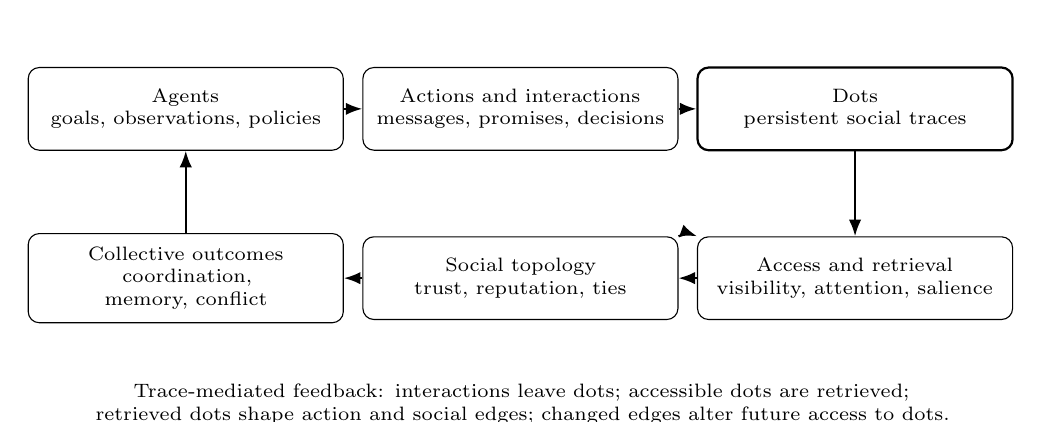
\begin{tikzpicture}[
  x=1cm,y=1cm,
  box/.style={draw, rounded corners, align=center, text width=3.65cm, minimum height=1.05cm, font=\scriptsize, inner sep=5pt},
  dotbox/.style={draw, rounded corners, thick, align=center, text width=3.65cm, minimum height=1.05cm, font=\scriptsize, inner sep=5pt},
  note/.style={align=center, font=\scriptsize, text width=10.8cm},
  arr/.style={-{Latex[length=2.1mm]}, thick}
]
\node[box] (agents) at (0,0) {Agents\\goals, observations, policies};
\node[box] (actions) at (4.25,0) {Actions and interactions\\messages, promises, decisions};
\node[dotbox] (dots) at (8.5,0) {Dots\\persistent social traces};
\node[box] (access) at (8.5,-2.15) {Access and retrieval\\visibility, attention, salience};
\node[box] (topology) at (4.25,-2.15) {Social topology\\trust, reputation, ties};
\node[box] (outcomes) at (0,-2.15) {Collective outcomes\\coordination, memory, conflict};
\draw[arr] (agents) -- (actions);
\draw[arr] (actions) -- (dots);
\draw[arr] (dots) -- (access);
\draw[arr] (access) -- (topology);
\draw[arr] (topology) -- (outcomes);
\draw[arr] (outcomes) -- (agents);
\draw[arr] (topology.north east) to[bend left=20] (access.north west);
\node[note] at (4.25,-3.75) {Trace-mediated feedback: interactions leave dots; accessible dots are retrieved; retrieved dots shape action and social edges; changed edges alter future access to dots.};
\end{tikzpicture}%
}
\caption{Conceptual overview of Dot-Trace Theory. Persistent social traces are first-class objects in the loop connecting agents, interaction, memory, and social topology. The figure separates dot creation from later access and retrieval, because a trace can persist even when it is not immediately used.}
\label{fig:conceptual-overview}
\end{figure}


The representational issue can be stated formally. Let
\[
Z_t=(A,E_t,X_t,\bar S_t)
\]
be a reduced state containing agents, social edges, environment, and ordinary non-dot state variables. If two systems share the same reduced state but differ in accessible traces, and if those traces affect future action, then the reduced state is not transition-sufficient. Dot-Trace Theory introduces a richer state representation that makes trace structure explicit and specifies when that richer representation is necessary.

The theory does not claim that memory, social networks, events, collective memory, or social capital are new. Its contribution is a coupling claim. Dots function simultaneously as event traces, memory objects, social artifacts, evidential objects, reputational supports, institutional records, and topology-changing causal elements. Treating them as first-class objects allows one to analyze how memory, action, and social structure co-evolve in human, artificial, and hybrid agent systems.

\section{Contributions and Scope}\label{contributions-scope}

The article contributes a formal vocabulary and theory for trace-mediated social systems. Its contributions are organized around representation, dynamics, consequences, and operationalization.

\begin{enumerate}[leftmargin=*,label=\textbf{C\arabic*.}]
\item \textbf{Trace primitive.} The article defines the dot as a persistent, socially situated memory-trace with content, provenance, context, salience, credibility, accessibility, lifecycle status, and relations to other dots.
\item \textbf{Dot-field state.} It defines the dot field as a coupled structure containing agents, social edges, dots, dot-dot relations, access relations, memory weights, effective strengths, provenance, institutional anchors, and correction states.
\item \textbf{Representation result.} It shows that reduced agent-edge projections can be insufficient for memory-sensitive systems unless the reduced representation encodes a dot-sufficient statistic.
\item \textbf{State-lifting result.} It shows that a dot-augmented state can restore Markov-style sufficiency when it encodes all transition-relevant history.
\item \textbf{Dynamic model.} It formalizes dot creation, retrieval, transmission, mutation, compression, institutionalization, counter-dot correction, lifecycle update, and topology feedback as operators on a common state space.
\item \textbf{Collective-memory consequences.} It derives conditions for dot consensus, fragmentation, temporal sequencing effects, institutional stabilization, and recursive topology-feedback stability.
\item \textbf{Social-capital interpretation.} It treats bonding, bridging, reputation, archival access, semantic brokerage, correction capacity, and liability as dot-mediated social-capital components.
\item \textbf{Operationalization.} It provides measurement, identifiability, algorithmic implementation, simulator, calibration, and validation protocols for applying the theory to observable or instrumented systems.
\end{enumerate}

The theory applies most directly to systems in which traces persist beyond their originating events; agents differ in access to those traces; traces can be retrieved, transmitted, corrected, institutionalized, or transformed; and social ties influence future trace exposure. It is less useful when the system is effectively memoryless, when all transition-relevant history is already encoded in a sufficient reduced state, or when trace variables cannot be observed, inferred, or experimentally manipulated with adequate discipline.

Three boundaries are central. First, a dot is not automatically true, beneficial, or morally legitimate. A false accusation, inaccurate record, or biased institutional label can be a dot if it persists and affects action. Second, a dot is not automatically a centroid of the social graph. Some dots can become centroid-like memory hubs in a lifted heterogeneous graph, but centrality is a derived property rather than a definition. Third, social capital is not itself a dot. It is a resource that can be accumulated, stabilized, transmitted, or destroyed through dot histories.

\section{Summary of the Argument}\label{summary-of-the-argument}

The argument can be stated in a compact sequence. First, many social multi-agent systems are trace-mediated: events leave persistent records, recollections, claims, commitments, accusations, summaries, or institutional entries that continue to matter after the event itself has ended. These traces are not interchangeable with ordinary social edges. A trust edge may summarize prior experience, but it does not by itself identify which trace is accessible, which source produced it, whether a counter-trace exists, or whether the trace has been institutionalized.

Second, if agents are memory-sensitive, then a reduced representation containing only agents, social edges, environmental variables, and non-dot internal state may be transition-insufficient. Two systems can share the same reduced state while differing in accessible traces. If those traces change future action probabilities, the reduced state cannot support the same transition law in both systems. The first role of Dot-Trace Theory is therefore representational: it identifies the additional state variables required when trace-mediated history remains causally relevant.

Third, the dot field supplies that state augmentation. It represents agents, dots, social edges, dot-dot relations, and agent-dot access relations, and its augmented form also records memory weights, effective retrievable strength, lineage, institutional stores, and correction states. The theory does not require every past event to be stored verbatim. It requires only that the current state preserve the historical distinctions that remain relevant for future action, coordination, correction, and topology change.

Fourth, once dots are treated as first-class objects, several mechanisms become formally visible. Dots may be created by events, retrieved by agents, transmitted through social ties, mutated by retelling, compressed into summaries, stabilized by institutions, challenged by counter-dots, and used to update trust or reputation. These mechanisms are not independent additions. They form a recursive system in which social edges determine access to traces, retrieved traces shape action and edge pressure, and updated edges alter future access.

Finally, the theory is operational only when its objects can be measured, inferred, logged, or experimentally manipulated with discipline. Dot-Trace Theory therefore pairs its formal claims with measurement rules, identifiability conditions, validation baselines, negative controls, and governance constraints. Its empirical burden is not to show that traces exist; the burden is to show that dot-field variables add explanatory, predictive, or interventional value beyond appropriate reduced-state baselines.

\section{Theoretical Scope and Testable Claim}\label{theoretical-scope-testable-claim}

The central formal claim is conditional. Dot-field representations matter when omitted trace variables remain relevant after conditioning on the reduced state. For an outcome $Y_{t+1}$, the core testable expression is
\[
I(Y_{t+1};D_t,R_t^D,B_t,\mathbf M_t,Q_t,L_t\mid A,E_t,X_t,\bar S_t)>0.
\]
When this conditional mutual information is positive, the dot field contains predictive information not present in the reduced agent-edge state. When it is zero for the outcome and time horizon under study, dot-field variables may still be descriptively meaningful, but they are not predictively necessary for that task.

This conditional formulation prevents overextension. The article establishes formal conditions under which dots are representationally necessary, dynamically consequential, measurable, or identifiable. It does not assert that every social system requires a dot-field model. The empirical burden in any application is to show that trace variables add explanatory, predictive, or interventional value beyond appropriate baselines.

\subsection{Article structure}\label{article-structure}

The argument proceeds in four layers. The first layer establishes the conceptual and formal vocabulary: the related-work section identifies the representational gap, and Sections~\ref{notation-state-hierarchy}--\ref{formal-dynamics} define the state hierarchy, dot ontology, dot field, dot types, axioms, and elementary dynamics. The second layer develops the process model: Sections~\ref{integrated-mixed-mechanism-dynamics} and~\ref{recursive-topology-feedback-stability} specify how retrieval, transmission, mutation, institutionalization, correction, and topology feedback operate within a common transition system. The third layer gives the main theoretical spine: representational insufficiency, Markov-style restoration, consensus and fragmentation, temporal sequencing, mixed-mechanism well-definedness, and recursive feedback stability. The fourth layer turns the theory outward, developing measurement rules, implementation architecture, validation protocols, applications, governance constraints, limitations, and terminology.

Because the theory spans representation, dynamics, measurement, and implementation, readers may follow different paths through the manuscript. Readers interested primarily in the formal contribution should focus on Sections~\ref{core-concept-the-dot}--\ref{theoretical-results}. Readers interested in application and operationalization should read the ontology and state hierarchy first, then proceed to Sections~\ref{measurement-dot-extraction-protocol}, \ref{experimental-validation-and-benchmarking-protocol}, and \ref{applications}. Readers interested in computational implementation can move from the integrated dynamics section directly to Sections~\ref{algorithmic-implementation}--\ref{trainable-prediction-negative-control-estimation}. The sections are ordered to support both a complete reading and targeted consultation of the theory's formal, empirical, and computational layers.

\begin{table}[htbp]
\centering
\small
\begin{tabular}{L{0.22\textwidth}L{0.34\textwidth}L{0.34\textwidth}}
\toprule
\textbf{Reader goal} & \textbf{Primary sections} & \textbf{What those sections establish}\\
\midrule
Understand the theory & Ontology, dot field, axioms, formal dynamics & What dots are, how they differ from messages, memories, and edges, and why they belong in the state representation.\\
Follow the proofs & Theorem consolidation and main theoretical results & Why reduced states can fail, how dot fields restore sufficiency under assumptions, and when memory converges, fragments, sequences, or feeds back into topology.\\
Apply the framework & Measurement, identifiability, validation, and applications & How to code dots, observe access, define baselines, test prediction lift, and apply the framework responsibly.\\
Implement the model & Integrated dynamics, algorithmic implementation, simulator, and calibration & How to turn the theory into a typed computational architecture with audit logs, calibration discipline, and validation outputs.\\
\bottomrule
\end{tabular}
\caption{Reading paths through the manuscript. The table distinguishes conceptual, formal, operational, and computational uses of Dot-Trace Theory.}
\label{tab:reading-paths}
\end{table}

\section{Related Work and Positioning}\label{related-work-and-positioning}

Dot-Trace Theory is adjacent to several mature literatures. The purpose of this section is not to claim priority over those literatures. It is to specify the representational gap that motivates the theory and to identify what is inherited from prior work versus what is introduced here.

\subsection{Name boundary: existing uses of ``Dot Theory''}\label{name-boundary-existing-dot-theory}

The name boundary matters. The phrase ``Dot Theory'' has existing uses, including the structured-representation program described by \citet{vossenDotTheory}. That program treats dots as discrete informational or contextual units in a representational system. Dot-Trace Theory uses a different primitive: the dot is a persistent, socially situated memory-trace with provenance, access, retrieval, credibility, lifecycle status, and possible effects on social topology. The present article therefore uses the more specific term \emph{Dot-Trace Theory} to avoid conflating the proposed framework with existing uses of the shorter name.

\subsection{Dynamic graph learning and event-based network models}\label{dynamic-graph-learning-event-based-models}

Dynamic graph learning provides an important technical neighbor because social systems are often represented as time-varying graphs. Temporal Graph Networks model dynamic graphs as sequences of timed events and combine memory modules with graph operators to support prediction on evolving networks \citep{rossi2020temporal}. Related dynamic-graph approaches treat events, edges, temporal neighborhoods, and node embeddings as central modeling objects.

Recent dynamic-graph surveys emphasize that temporal graph learning now includes continuous-time interaction graphs, dynamic GNN architectures, benchmark libraries, temporal link prediction, and large-scale training challenges \citep{zheng2024dynamicgnn,jiao2025temporalinteraction,yu2023dygformer,feng2024dynamicgnn}. These literatures are important because they show how much can be learned from event sequences and evolving edges. They also sharpen the boundary of the present theory: Dot-Trace Theory is not a new dynamic graph neural network. It is a representational theory for cases in which the objects created by events remain socially meaningful after the event and can later be retrieved, contested, institutionalized, or used to change the edge structure itself.


Dot-Trace Theory is compatible with this perspective but differs in its ontology. In a dynamic graph, an event updates node or edge representations. In Dot-Trace Theory, an event may also create a persistent trace with content, provenance, accessibility, credibility, relations, mutation history, and future causal force. Thus, a dot is not merely an event timestamp or a hidden node memory; it is a social-memory object that can be retrieved, transmitted, contested, institutionalized, or used to modify future topology.

\subsection{Agent memory and generative agents}\label{agent-memory-generative-agents-graph-memory}

Long-term memory has become a central design problem for LLM-enabled agents and interactive simulations. Generative agents store natural-language records of experience, retrieve relevant memories, synthesize reflections, and use those memories to plan behavior \citep{park2023generative}. MemoryBank introduces long-term memory for LLM interactions with reinforcement and forgetting mechanisms inspired by human memory \citep{zhong2024memorybank}. MemGPT frames memory management as virtual context management across tiers, addressing the limited context window of language models \citep{packer2023memgpt}. A-MEM proposes an agentic memory architecture that dynamically organizes memories as interconnected notes with structured attributes \citep{xu2025amem}.

Recent surveys of LLM-agent memory further stress that agent memory cannot be reduced to a single short-term/long-term distinction: it involves formation, storage substrate, retrieval control, updating, summarization, evaluation, and governance \citep{zhang2024memorysurvey,hu2025memoryage,luo2026storageexperience}. Production-oriented systems such as Mem0 also illustrate the practical pressure for scalable long-term memory in agentic applications \citep{mem02025}. Empirical work on memory management further shows that addition, deletion, and retrieval policies can materially change LLM-agent behavior, error propagation, and robustness over time \citep{xiong2025memorymanagement}. Dot-Trace Theory takes these developments as evidence that memory is becoming an explicit design object, but it insists that social accessibility, provenance, and topology feedback must be modeled when memory-bearing agents interact.


These systems show that memory is operationally important for believable and coherent agents. Dot-Trace Theory adds a social state layer to this line of work. It asks how memory records become distributed across agents, artifacts, and institutions; how agents gain or lose access to them; how retrieved traces shape social edges; and how traces mutate, compress, or become contested across a population. The difference is not that prior agent-memory systems lack memory. The difference is that Dot-Trace Theory makes trace access, trace transmission, and trace-induced topology feedback explicit objects of theory.

\subsection{Graph-based agent memory and graph-augmented agents}\label{graph-based-agent-memory}

Graph-based memory is especially close to the present framework. Recent surveys argue that graphs can organize relational dependencies, hierarchical information, retrieval pathways, and memory evolution in LLM agents \citep{yang2026graphmemory}. Broader graph-agent surveys likewise argue that graph structures can support agent planning, execution, memory, and multi-agent coordination \citep{bei2025graphsmeet,liu2025graphaugmented}.

Dot-Trace Theory adopts the insight that memory is often relational, but it distinguishes three graph layers that are frequently collapsed in implementation work:
\[
G^A_t=(A,E_t),\qquad G^D_t=(D_t,R_t^D),\qquad G^B_t=(A,D_t,B_t).
\]
The first is the social graph among agents, the second is the dot graph among traces, and the third is the access graph between agents and traces. This separation is central. A graph-memory node can be useful for retrieval; a dot can additionally be inaccessible to some agents, credible to others, institutionally anchored, semantically mutated, or capable of changing the social edge through which future memories travel.

\subsection{LLM-agent societies and synthetic social systems}\label{llm-agent-societies-synthetic-systems}

LLM-agent societies and social simulation systems provide a natural application domain. Surveys of LLM-driven and LLM-empowered social simulation distinguish individual simulation, scenario simulation, and society-scale simulation, while also emphasizing calibration, human alignment, evaluation, and methodological scope conditions \citep{gao2024llmabm,mou2024socialsimulation}. Large-scale systems such as AgentSociety use LLM-driven generative agents and social environments to simulate interactions relevant to polarization, inflammatory messages, policy shocks, and social behavior \citep{piao2025agentsociety}. Position papers on LLM-based social simulation also emphasize the need for boundary-aware validation and careful claim discipline, particularly when heterogeneity, behavioral variance, social realism, scheduling, and environment-agent co-dynamics matter \citep{wu2025boundary,li2026notpanacea}.

More recent work on LLMs in agent-based social simulation emphasizes calibration, reproducibility, behavioral fidelity, subgroup reliability, and the risk of treating plausible language outputs as direct evidence of social mechanisms \citep{taillandier2025integrating,madden2025synthetic}. Large-scale world-model efforts such as SocioVerse further demonstrate the scale at which synthetic social environments are being built, while also making trace governance, data provenance, and validation more important \citep{zhang2025socioverse}. These developments motivate Dot-Trace Theory's insistence on audit logs, negative controls, and observability grades.


Dot-Trace Theory contributes a representation layer for such systems. Synthetic agents often produce messages, posts, records, summaries, tool logs, and public artifacts. The theory supplies criteria for when those artifacts should be treated as persistent social traces, how access to them should be modeled, how they become memory for agents, and how they affect later interaction. It also constrains claims: a synthetic society with messages but no trace retrieval, no access structure, and no topology feedback is not a strong test of Dot-Trace Theory.

\subsection{Collective memory and social-network topology}\label{collective-memory-social-network-topology}

Collective memory research provides the strongest conceptual precedent for the social side of the theory. Bartlett's work emphasized reconstructive remembering and schema-shaped recall \citep{bartlett1932remembering}. Halbwachs argued that memory is situated in collective frameworks rather than isolated individual storage \citep{halbwachs1992collective}. Experimental work on mnemonic convergence shows that communication in networks can align memories and that bridge ties and conversation timing can affect collective memory formation \citep{coman2016mnemonic,momennejad2019bridge}. \citet{momennejad2022collective} reviews evidence that social-network topology shapes collective cognition. Recent digital-memory work further emphasizes how social media and platformization reshape remembering and forgetting through algorithmic curation and connective practices \citep{adriaansen2025collective}.

Dot-Trace Theory formalizes a mechanism beneath these phenomena. Collective memory is represented as structured overlap and weighting over accessible dots, not merely as shared belief or narrative similarity. Bridge ties matter because they transmit dots across components. Conversation timing matters because dot-assimilation operators may be non-commutative. Platform curation matters because it changes access, visibility, salience, and retrieval probabilities. Institutional records matter because they stabilize particular dots and increase correction costs.

\subsection{Consensus, opinion dynamics, and social influence}\label{consensus-opinion-dynamics-social-influence}

Consensus and social influence models provide a mathematical basis for several results in this article. DeGroot's model formalizes convergence through repeated averaging over an influence matrix \citep{degroot1974reaching}. Friedkin and Johnsen's model incorporates interpersonal influence and persistent individual susceptibilities, allowing stable disagreement under some conditions \citep{friedkin1990social}.

Dot-Trace Theory uses this mathematical lineage but changes the unit being updated. Agents do not only update scalar opinions. They update dot weights, credibility, salience, accessibility, and relations over structured traces. As a result, two populations can share the same influence graph but diverge because they access different dots, retrieve different counter-dots, trust different institutional anchors, or compress the same history into different reputational summaries.

\subsection{Social capital, brokerage, and weak ties}\label{social-capital-brokerage-weak-ties}

Social capital theory is central to the interpretation of dot access. Bourdieu defines social capital as resources linked to durable networks of acquaintance and recognition \citep{bourdieu1986forms}. Coleman emphasizes obligations, expectations, trustworthiness, information channels, and norms as resources that facilitate action \citep{coleman1988social}. Putnam popularizes bonding and bridging forms of social capital in civic life \citep{putnam2000bowling}. Granovetter's weak-tie argument shows how bridging ties move information across clusters \citep{granovetter1973strength}, and Burt's structural-holes theory analyzes brokerage advantages between disconnected others \citep{burt1992structural}. Nahapiet and Ghoshal connect social capital to intellectual capital and organizational advantage \citep{nahapiet1998social}, while Lin develops a network theory of social resources \citep{lin2001social}.

Dot-Trace Theory does not replace social capital theory. It supplies a trace-level substrate for some of its mechanisms. A tie can be valuable because it grants access to useful dots. A broker can be valuable because they control which dots cross social boundaries and how those dots are translated. Reputation capital can accumulate through favorable evaluative dots. Social liability can accumulate through negative, false, obsolete, or exclusionary dots. Bridging capital can prevent threshold closure by keeping corrective dots reachable after ordinary trust edges collapse. In this sense, social capital is a derived advantage; dots are the memory-trace objects through which much of that advantage is produced, circulated, stabilized, or destroyed.

\subsection{Organizational and institutional memory}\label{organizational-institutional-memory}

Organizational memory research is another close neighbor. \citet{walsh1991organizational} conceptualize organizational memory as retained information from an organization's history that can influence present decisions. \citet{argote2013organizational} examines organizational learning as creating, retaining, and transferring knowledge. Boundary-object theory shows how artifacts can coordinate action across social worlds without requiring identical meanings for every group \citep{star1989institutional}.

Dot-Trace Theory reframes institutional memory as dot stabilization. Meeting minutes, tickets, audit logs, policies, contracts, issue histories, and archives are institutional dots when they persist, remain accessible, and influence later action. Institutionalization can increase reach, credibility, synchronization, and half-life; it can also stabilize false, biased, obsolete, or incomplete traces. This is why institutional dots are treated as both coordination resources and possible sources of durable harm.

\subsection{Identifiability, causal inference, and validation}\label{identifiability-causal-inference-validation}

Because dots are often partially observed or latent, the theory must be tied to identifiability and validation. Pearl's intervention framework distinguishes association from causal effect \citep{pearl2009causality}. Constraint-based causal discovery and latent-structure work show that distinct hidden structures can generate the same observable distribution \citep{spirtes2000causation}. Proper scoring-rule theory provides a principled basis for comparing probabilistic predictions \citep{gneiting2007proper}.

The implication is methodological. Dot-field claims must be indexed by observability. Action-only data may reveal aggregate pressure but not dot composition. Communication logs may reveal trace tokens but not attention or retrieval. Access logs may reveal exposure but not belief. Randomized exposure can identify causal effects under stronger conditions. The measurement, identifiability, and validation sections of this article therefore treat dot extraction as a scientific measurement problem rather than a clerical preprocessing step.

This methodological stance is also reinforced by emerging security and governance work on long-term memory in LLM agents. When memories can persist, be retrieved, be poisoned, be extracted, or travel across agents, memory becomes not only a performance feature but a risk surface \citep{securitymemory2026}. Dot-Trace Theory therefore treats provenance, correction, contestability, and lifecycle governance as part of the formal model rather than as external implementation details.


\subsection{Positioning map}\label{positioning-map}

Figure~\ref{fig:literature-positioning-map} summarizes the positioning. Dot-Trace Theory is not offered as a replacement for the adjacent literatures. It is a coupling theory whose primitive object links the layers those literatures often study separately.

\begin{figure}[htbp]
\centering
\resizebox{0.98\textwidth}{!}{%
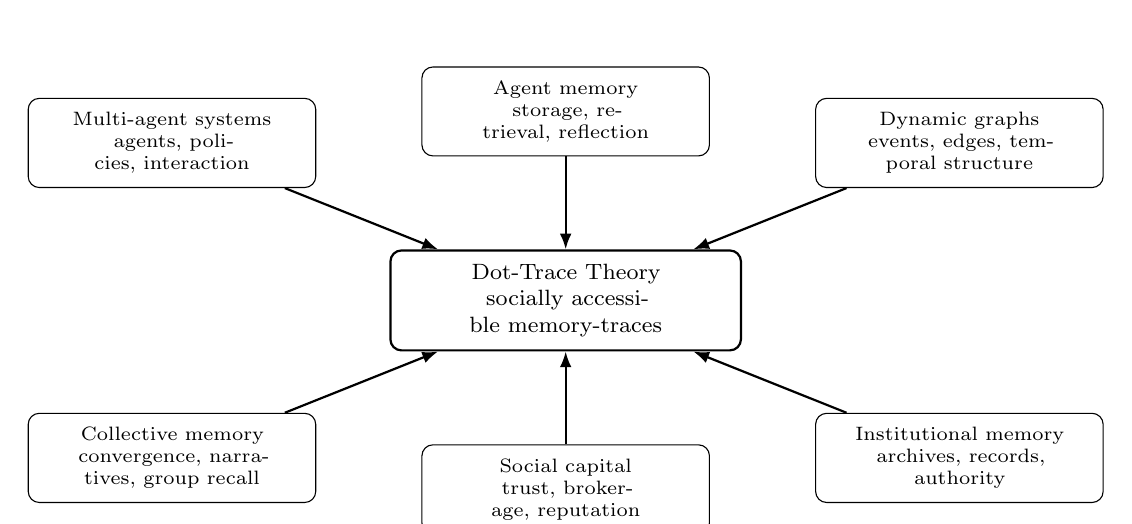
\begin{tikzpicture}[
  x=1cm,y=1cm,
  core/.style={draw, rounded corners, thick, align=center, text width=4.1cm, minimum height=1.15cm, font=\footnotesize, inner sep=5pt},
  field/.style={draw, rounded corners, align=center, text width=3.3cm, minimum height=1.05cm, font=\scriptsize, inner sep=5pt},
  arr/.style={-{Latex[length=2.0mm]}, thick}
]
\node[core] (dtt) at (0,0) {Dot-Trace Theory\\socially accessible memory-traces};
\node[field] (mas) at (-5.0,2.0) {Multi-agent systems\\agents, policies, interaction};
\node[field] (memory) at (0,2.4) {Agent memory\\storage, retrieval, reflection};
\node[field] (graphs) at (5.0,2.0) {Dynamic graphs\\events, edges, temporal structure};
\node[field] (collective) at (-5.0,-2.0) {Collective memory\\convergence, narratives, group recall};
\node[field] (capital) at (0,-2.4) {Social capital\\trust, brokerage, reputation};
\node[field] (institution) at (5.0,-2.0) {Institutional memory\\archives, records, authority};
\foreach \x in {mas,memory,graphs,collective,capital,institution}{\draw[arr] (\x) -- (dtt);}
\end{tikzpicture}%
}
\caption{Positioning map. Dot-Trace Theory is a coupling theory: it imports agents, memories, events, networks, institutions, and social resources from adjacent literatures, then introduces the socially accessible trace as the object connecting those layers.}
\label{fig:literature-positioning-map}
\end{figure}


\subsection{Consolidated positioning}\label{consolidated-positioning}

The relationship among adjacent literatures can be summarized as follows.

{\small
\begin{longtable}{L{0.20\textwidth}L{0.28\textwidth}L{0.34\textwidth}}
\caption{How Dot-Trace Theory is positioned relative to adjacent literatures.}\label{tab:literature-positioning}\\
\toprule
\textbf{Adjacent area} & \textbf{What it contributes} & \textbf{What Dot-Trace Theory adds}\\
\midrule
\endfirsthead
\toprule
\textbf{Adjacent area} & \textbf{What it contributes} & \textbf{What Dot-Trace Theory adds}\\
\midrule
\endhead
Dynamic graph learning & Timed events, evolving edges, node memory, prediction on dynamic graphs. & Persistent trace objects with provenance, access, credibility, lifecycle, mutation, correction, and topology feedback.\\
Agent memory and generative agents & Experience storage, reflection, retrieval, planning, long-term interaction. & Distribution of traces across agents, artifacts, institutions, and social access paths.\\
Graph-based memory & Relational memory structures and graph-based retrieval. & Separate agent-agent, dot-dot, and agent-dot access graphs, with dots as social and causal objects.\\
LLM-agent societies & Scalable synthetic interaction, agent roles, communication, social simulation. & Criteria for when messages and artifacts become persistent traces and how those traces shape future social dynamics.\\
Collective memory & Shared remembering, mnemonic convergence, group narratives, digital memory. & Formal dot overlap, access, bridge timing, counter-dots, institutional anchors, and fragmentation metrics.\\
Opinion dynamics & Influence matrices, consensus, disagreement, social influence. & Structured dot weights, credibility, salience, access, and retrieval rather than scalar opinions alone.\\
Social capital & Resources through ties, trust, brokerage, bonding, bridging, reputation. & Memory-trace substrate through which those resources are accumulated, transferred, repaired, or destroyed.\\
Organizational memory & Retention, transfer, routines, records, institutional repositories. & Institutional dots as persistence, reach, authority, correction-cost, and capture mechanisms.\\
Causal inference and validation & Identifiability, interventions, predictive evaluation, negative controls. & Observability ladder and theorem-to-measurement compatibility for dot-field claims.\\
\bottomrule
\end{longtable}
}

The gap motivating Dot-Trace Theory can therefore be stated precisely:

\begin{quote}
Existing work models agents, memories, events, social ties, institutions, and social resources in powerful but often separated frameworks. Dot-Trace Theory treats the socially accessible memory-trace as the bridge object through which these layers can be represented in one state space.
\end{quote}

This is a coupling claim, not a priority claim. The originality of the theory lies in making the dot a first-class object and formalizing its access, retrieval, transmission, mutation, correction, institutionalization, and topology-changing consequences.

\section{Notation and State Hierarchy}\label{notation-state-hierarchy}

The theory uses several levels of representation. A reduced social-network model may contain only agents, edges, environment, and ordinary state variables. A core dot field adds dots, dot-dot relations, and access relations. An augmented dot field adds weights, effective strengths, lineage, institutions, and correction state. An executable implementation state adds indexes, logs, and runtime metadata. This section fixes the canonical notation for these levels.

\subsection{State levels}\label{state-levels}

The reduced agent-edge representation is
\[
Z_t=(A,E_t,X_t,\bar S_t),
\]
where $A$ is the agent set, $E_t$ is the agent-agent social graph, $X_t$ is the environmental state, and $\bar S_t$ denotes ordinary non-dot internal or contextual state variables that a reduced model may include.

The core dot field is
\[
\Omega_t^{core}=(A,E_t,X_t,\bar S_t,D_t,R_t^D,B_t),
\]
where $D_t$ is the dot set, $R_t^D\subseteq D_t\times D_t$ is the dot-dot relation structure, and $B_t\subseteq A\times D_t$ is the agent-dot access relation.

The augmented dot field is
\[
\Omega_t^{aug}=(\Omega_t^{core},\mathbf M_t,Q_t,L_t,I_t,C_t),
\]
where $\mathbf M_t$ is the dot-weight matrix, $Q_t$ contains effective retrievable strengths, $L_t$ records provenance or lineage, $I_t$ denotes institutional stores or anchors, and $C_t$ denotes counter-dot and correction state.

The executable implementation state is
\[
\mathsf S_t=(\Omega_t^{aug},\mathsf{Idx}_t,\mathsf{Log}_t,\mathsf{Meta}_t),
\]
where $\mathsf{Idx}_t$ are retrieval and storage indexes, $\mathsf{Log}_t$ is the audit log, and $\mathsf{Meta}_t$ contains implementation metadata such as permissions, runtime configuration, and validation flags.


\begin{figure}[htbp]
\centering
\resizebox{0.96\textwidth}{!}{%
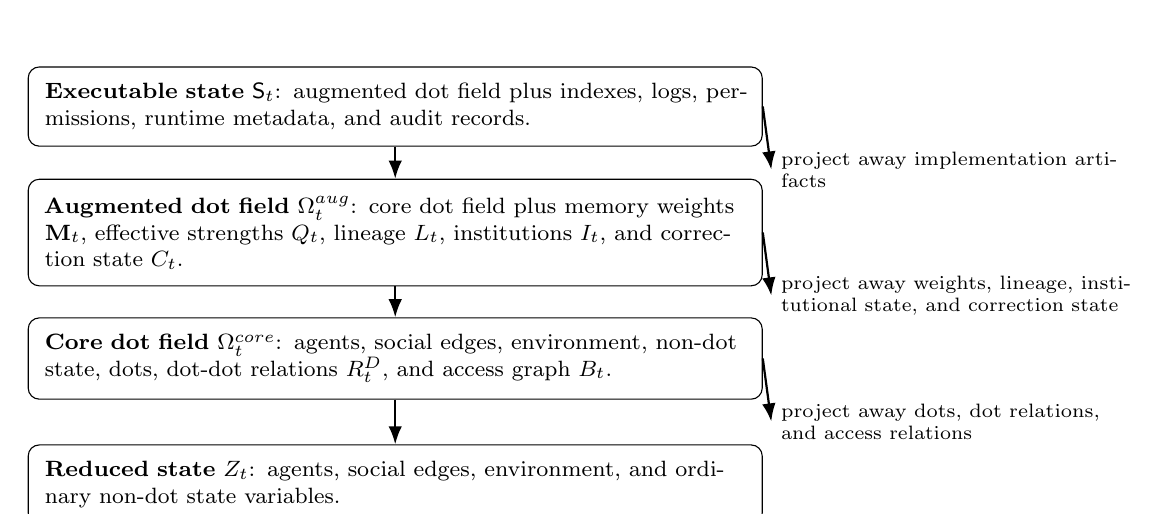
\begin{tikzpicture}[
  x=1cm,y=1cm,
  state/.style={draw, rounded corners, align=left, text width=8.9cm, minimum height=0.95cm, font=\footnotesize, inner sep=6pt},
  loss/.style={align=left, text width=4.4cm, font=\scriptsize},
  arr/.style={-{Latex[length=2.3mm]}, thick}
]
\node[state] (S) at (0,0) {\textbf{Executable state} $\mathsf S_t$: augmented dot field plus indexes, logs, permissions, runtime metadata, and audit records.};
\node[state] (A) at (0,-1.6) {\textbf{Augmented dot field} $\Omega_t^{aug}$: core dot field plus memory weights $\mathbf M_t$, effective strengths $Q_t$, lineage $L_t$, institutions $I_t$, and correction state $C_t$.};
\node[state] (C) at (0,-3.2) {\textbf{Core dot field} $\Omega_t^{core}$: agents, social edges, environment, non-dot state, dots, dot-dot relations $R_t^D$, and access graph $B_t$.};
\node[state] (Z) at (0,-4.8) {\textbf{Reduced state} $Z_t$: agents, social edges, environment, and ordinary non-dot state variables.};
\node[loss] (l1) at (7.1,-0.8) {project away implementation artifacts};
\node[loss] (l2) at (7.1,-2.4) {project away weights, lineage, institutional state, and correction state};
\node[loss] (l3) at (7.1,-4.0) {project away dots, dot relations, and access relations};
\draw[arr] (S) -- (A);
\draw[arr] (A) -- (C);
\draw[arr] (C) -- (Z);
\draw[arr] (S.east) -- (l1.west);
\draw[arr] (A.east) -- (l2.west);
\draw[arr] (C.east) -- (l3.west);
\end{tikzpicture}%
}
\caption{Canonical state hierarchy. Each projection removes structure. The central representational question is whether the removed structure is transition-relevant for the outcome and horizon being modeled.}
\label{fig:state-hierarchy}
\end{figure}


\subsection{Projection and information loss}\label{projection-information-loss}

The relationship among state levels is represented by projections:
\[
\mathsf S_t \to \Omega_t^{aug} \to \Omega_t^{core} \to Z_t.
\]
Each projection removes structure. Moving from $\mathsf S_t$ to $\Omega_t^{aug}$ removes implementation metadata, indexes, and logs. Moving from $\Omega_t^{aug}$ to $\Omega_t^{core}$ removes auxiliary variables such as memory weights, lineages, institutional stores, and correction state. Moving from $\Omega_t^{core}$ to $Z_t$ removes the explicit dot layer itself. The central representational question is whether any removed structure is transition-relevant.

For an outcome $Y_{t+1}$, the projection loss from the augmented dot field to the reduced agent-edge state can be written as
\[
\mathcal L_{proj}(Y_{t+1};\Omega_t^{aug}\to Z_t)
=I(Y_{t+1};\Omega_t^{aug}\mid Z_t).
\]
If this quantity is zero, the omitted dot-field variables add no predictive information for the specified outcome and horizon. If it is positive, a reduced representation has lost transition-relevant trace information. Projection loss is therefore the information-theoretic form of the theory's core claim: dots matter only when their omission changes what can be predicted, explained, or controlled.

\subsection{Retrieval notation}\label{retrieval-notation}

To avoid ambiguity, the article distinguishes dot-dot relations from retrieved dot sets. Dot-dot relations are denoted by $R_t^D$. The set or sequence of dots retrieved by agent $a_i$ for query or decision context $q$ is denoted by
\[
\mathcal V_i(q,t)\subseteq \mathcal M_i(t),
\]
where $\mathcal M_i(t)=\{d\in D_t:(a_i,d)\in B_t\}$ is the set of dots accessible to agent $a_i$. The notation $R_t^D$ is reserved for dot-dot relations, while $\mathcal V_i(q,t)$ denotes retrieved dots.

This distinction is small but consequential. A dot may be connected to many other dots in $R_t^D$ without being retrieved by any agent in a particular decision. Conversely, an agent may retrieve a dot without traversing the entire dot graph. The empirical equivalents are also different: a database can reveal dot-dot relations, an access log can reveal reachability, and a retrieval log can reveal decision-context activation. Treating these objects as interchangeable would weaken the theory's measurement discipline.

\subsection{Cross-section terminology convention}\label{cross-section-terminology-convention}

The article uses a small number of terms with fixed meanings across the conceptual, formal, measurement, implementation, and validation sections. A \emph{dot} is the trace object. A \emph{dot field} is the state representation containing agents, social edges, dots, dot-dot relations, and access relations, with augmented variables added when retrieval weights, lineages, institutions, or correction states are required. The \emph{reduced state} is always denoted $Z_t$ and contains only the agent-edge and non-dot variables available to a dot-free model. Dot-induced edge pressure is denoted by $\zeta_{ij}(t)$ or by the matrix $\boldsymbol{\zeta}_t$; the symbol $Z_t$ is not used for edge pressure.

This convention separates three concepts that are easy to collapse. \emph{Access} means that an agent can in principle obtain a dot, and is encoded by $B_t$ or by the accessible set $\mathcal M_i(t)$. \emph{Retrieval} means that an accessible dot enters a decision context, and is encoded by $\mathcal V_i(q,t)$. \emph{Influence} means that a retrieved dot changes action, memory, correction, reputation, or topology through its effective strength $Q_i(d,t)$ and any task-specific valence or relevance terms. Later measurement and validation sections preserve these distinctions: a dataset may observe communication without observing access, access without observing retrieval, or retrieval without separately identifying credibility and salience.

\subsection{Completeness condition}\label{dot-state-completeness}

The Markov-restoration claim later in the paper depends on a completeness condition:
\[
P(Y_{t+1}\mid \mathcal H_t)=P(Y_{t+1}\mid \Omega_t^{aug}),
\]
where $\mathcal H_t$ is the relevant historical process. The condition does not assert that dots magically make every system Markovian. It states that a dot-augmented state is sufficient only when it encodes all historical information relevant to the target transition.

Completeness is therefore both a theorem assumption and an empirical burden. In a formal model, the analyst specifies which historical variables are encoded by $D_t$, $R_t^D$, $B_t$, $\mathbf M_t$, $Q_t$, $L_t$, $I_t$, and $C_t$. In an empirical study, the analyst must justify why the observed or inferred dot field captures the trace variables needed for the claim. If an omitted historical factor continues to affect the outcome after conditioning on $\Omega_t^{aug}$, then the dot field is incomplete for that transition.


\section{Core Concept: The Dot}\label{core-concept-the-dot}

The dot is the conceptual and mathematical primitive of the theory. This section separates the dot from nearby notions--events, memories, messages, and edges--so that later formal results can rely on a stable object.

\subsection{Informal definition}\label{informal-definition}

A \textbf{dot} is a persistent trace of meaning left by an event, observation, interaction, claim, judgment, or record. It is a memory-bearing object with social position. Examples include traces such as ``Agent A helped Agent B,'' ``Agent C betrayed the group,'' ``this source is reliable,'' ``this meeting created an unresolved obligation,'' ``this document is the official version,'' or ``this behavior violated a group norm.'' These traces differ in content, credibility, reach, and durability, but each can persist beyond the originating moment and later affect action.

A dot is not identical to a message. A message is an act or content transmitted at a moment; a dot is the trace that may remain after the message is interpreted, stored, linked, and reused. A dot is not identical to a private memory. Some dots are private, but others are public, institutional, algorithmic, or distributed across many agents. A dot is not identical to a social edge. An edge connects agents; a dot provides memory-relevant content that may strengthen, weaken, create, or delete edges.

\subsection{Formal definition}\label{formal-definition}

\begin{definition}[Dot]
A dot $d_k$ is a structured memory-trace represented as
$$
d_k = \langle id_k, x_k, p_k, c_k, \tau_k, \sigma_k, \gamma_k, \alpha_k, \nu_k, \ell_k, \theta_k \rangle,
$$
where $id_k$ is a unique identifier, $x_k$ is semantic content, $p_k$ is provenance, $c_k$ is context, $\tau_k$ is time of creation, $\sigma_k$ is salience, $\gamma_k$ is credibility, $\alpha_k$ is affective or normative charge, $\nu_k$ is visibility or accessibility, $\ell_k$ is lifecycle state, and $\theta_k$ is a set of relations to other dots.
\end{definition}

The components have the following interpretation:

\begin{longtable}[]{@{}lll@{}}
\toprule\noalign{}
Component & Meaning & Example \\
\midrule\noalign{}
\endhead
\bottomrule\noalign{}
\endlastfoot
\(id_k\) & Unique identifier & Dot 1842 \\
\(x_k\) & Content & ``Agent B missed the deadline'' \\
\(p_k\) & Provenance & Observed by A; reported by C \\
\(c_k\) & Context & Project X, sprint 3, high pressure \\
\(\tau_k\) & Time & Creation time or event time \\
\(\sigma_k\) & Salience & Importance or retrieval strength \\
\(\gamma_k\) & Credibility & Confidence in truth or reliability \\
\(\alpha_k\) & Charge & Positive, negative, moral, affective \\
\(\nu_k\) & Visibility & Private, shared, public, institutional \\
\(\ell_k\) & Lifecycle & Active, decayed, reinforced, deleted \\
\(\theta_k\) & Links & Supports, contradicts, causes, generalizes \\
\end{longtable}

The theory is flexible about the internal representation of \(x_k\). The
content of a dot may be a natural-language statement, an event tuple, a
vector embedding, a logical proposition, a symbolic record, a database
entry, or a multimodal trace. The theory requires only that the content
can be stored, retrieved, compared, transmitted, and used in action
selection.

\subsection{Dot versus event}\label{dot-versus-event}

An event is a happening; a dot is the encoded aftermath of that happening. The distinction matters because an event may be momentary, unobserved, or forgotten, whereas a dot can continue to influence action after the event itself is no longer present. Formally, let \(e_t\) be an event at time \(t\). The dot creation function is
\[
d_{new} = \kappa(e_t,c_t),
\]
where \(c_t\) is the context of encoding. The mapping \(\kappa\) need not be one-to-one. A single event can create several dots because agents may witness different aspects of it, record it in different media, or attach different salience and credibility to it. Conversely, many events can be compressed into a single dot, such as an incident summary, a reputation label, or a recurring norm. Dot-Trace Theory is therefore not an event theory in disguise: the event explains origin, while the dot explains persistence, access, retrieval, and later causal force.

\subsection{Dot versus memory}\label{dot-versus-memory}

Memory is usually agent-centered: it concerns what an agent stores, forgets, retrieves, or believes. A dot is trace-centered: it concerns a persistent object that may be stored privately, shared socially, embedded institutionally, surfaced algorithmically, or contested by counter-dots. A private episodic memory can be represented as a dot when its content, provenance, access, and lifecycle matter for future behavior. But dots are not restricted to private cognition. Meeting minutes, rumors, reputation markers, legal records, social media posts, audit logs, shared stories, and database entries can also be dots. This distinction permits one theory to describe private memory, collective memory, institutional memory, and machine-readable memory without collapsing them into a single psychological category.

\subsection{Dot versus edge}\label{dot-versus-edge}

A social edge describes a relation between agents. A dot can explain why
that edge exists, why it changed, and how it is expected to change. For
example, if agent \(i\) trusts agent \(j\), a standard social graph may
encode \(w_{ij}^{trust}=0.8\). Dot-Trace Theory asks which dots support
that value: \[
\{d_1 = \text{j kept a promise}, d_2 = \text{j gave accurate advice}, d_3 = \text{j defended agent } i \text{ publicly}\}.
\] The social edge is therefore not only a number. It is dot-supported.




\begin{figure}[htbp]
\centering
\resizebox{0.98\textwidth}{!}{%
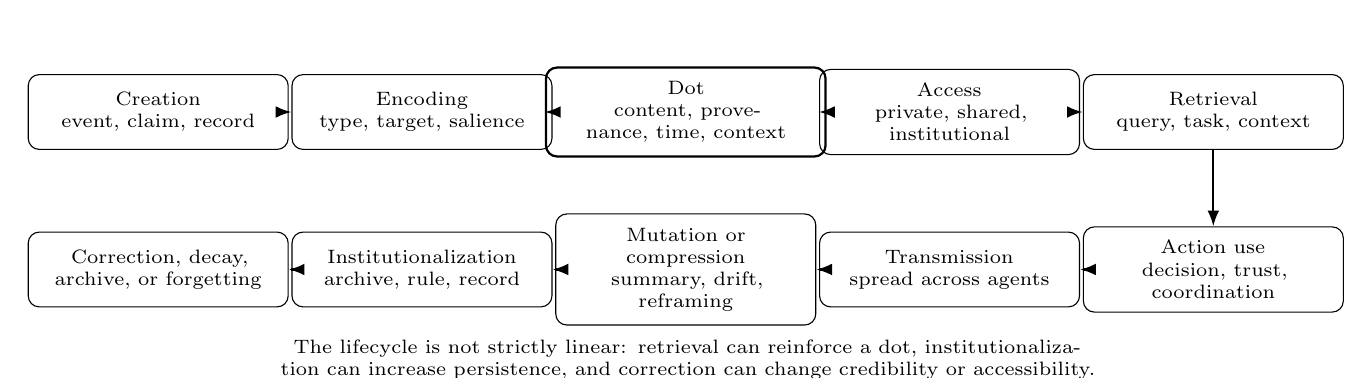
\begin{tikzpicture}[
  x=1cm,y=1cm,
  stage/.style={draw, rounded corners, align=center, text width=2.95cm, minimum height=0.95cm, font=\scriptsize, inner sep=5pt},
  core/.style={draw, rounded corners, thick, align=center, text width=3.2cm, minimum height=1.05cm, font=\scriptsize, inner sep=5pt},
  arr/.style={-{Latex[length=2.0mm]}, thick}
]
\node[stage] (create) at (0,0) {Creation\\event, claim, record};
\node[stage] (encode) at (3.35,0) {Encoding\\type, target, salience};
\node[core] (dot) at (6.7,0) {Dot\\content, provenance, time, context};
\node[stage] (access) at (10.05,0) {Access\\private, shared, institutional};
\node[stage] (retrieval) at (13.4,0) {Retrieval\\query, task, context};
\node[stage] (action) at (13.4,-2.0) {Action use\\decision, trust, coordination};
\node[stage] (transmit) at (10.05,-2.0) {Transmission\\spread across agents};
\node[stage] (mutate) at (6.7,-2.0) {Mutation or compression\\summary, drift, reframing};
\node[stage] (inst) at (3.35,-2.0) {Institutionalization\\archive, rule, record};
\node[stage] (decay) at (0,-2.0) {Correction, decay, archive, or forgetting};
\draw[arr] (create) -- (encode);
\draw[arr] (encode) -- (dot);
\draw[arr] (dot) -- (access);
\draw[arr] (access) -- (retrieval);
\draw[arr] (retrieval) -- (action);
\draw[arr] (action) -- (transmit);
\draw[arr] (transmit) -- (mutate);
\draw[arr] (mutate) -- (inst);
\draw[arr] (inst) -- (decay);
\node[align=center,font=\scriptsize,text width=11.5cm] at (6.7,-3.15) {The lifecycle is not strictly linear: retrieval can reinforce a dot, institutionalization can increase persistence, and correction can change credibility or accessibility.};
\end{tikzpicture}%
}
\caption{Lifecycle of a dot. A dot can be created, encoded, made accessible, retrieved, used in action, transmitted, mutated, compressed, institutionalized, corrected, decayed, archived, or forgotten. Feedback among these stages is represented conceptually rather than by crossing arrows, because the relevant feedback channels vary by domain.}
\label{fig:dot-lifecycle}
\end{figure}




\section{Dot Centrality, Centroids, and Social Capital}\label{dot-centrality-centroids-and-social-capital}

Dot-Trace Theory should not be read as claiming that a dot is, by definition, the centroid of a social network. A dot is a trace object. Centrality is a possible derived property of some dots, not the primitive definition of all dots.

In the ordinary social graph
\[
G_t^A=(A,E_t),
\]
vertices are agents. A centroid-like position in this graph is therefore an agent or a location defined over agent-agent relations. A dot is not a vertex of $G_t^A$. Dot-Trace Theory instead works with three coupled graphs:
\[
G_t^A=(A,E_t),\qquad G_t^D=(D_t,R_t^D),\qquad G_t^B=(A,D_t,B_t).
\]
The first is the social graph among agents. The second is the graph among traces. The third is the bipartite access graph connecting agents to the dots they can retrieve or encounter.

A dot can become centroid-like only after these graphs are lifted into a heterogeneous graph:
\[
H_t=(A\cup D_t,E_t\cup R_t^D\cup B_t).
\]
In $H_t$, both agents and dots are vertices. Some dots may then become memory hubs: founding documents, public accusations, canonical datasets, shared traumas, widely cited meeting records, or institutional rules may lie close to many agents and connect many trace relations. Most dots, however, remain peripheral, private, low-salience, or forgotten.

\begin{definition}[Group dot-centroid]
Let $G\subseteq A$ be a group of agents and let $H_t=(A\cup D_t,E_t\cup R_t^D\cup B_t)$ be the lifted heterogeneous graph. For weights $\lambda_i^G\geq 0$ with $\sum_{a_i\in G}\lambda_i^G=1$, a group dot-centroid is any dot
\[
d_G^*(t)\in\arg\min_{d\in D_t}\sum_{a_i\in G}\lambda_i^G\,\delta_t(a_i,d)^p,
\]
where $\delta_t(a_i,d)$ is a distance or access-cost measure in $H_t$ and $p\geq 1$.
\end{definition}

This definition separates three objects that are easy to conflate. The \emph{dot-centroid} $d_G^*(t)$ is a graph-geometric object in the lifted graph. The \emph{collective memory barycenter}
\[
\bar m_G(t)=\sum_{a_i\in G}\pi_i^G m_i(t)
\]
is a vector-space object over dot weights. A \emph{representative dot} $\widehat d_G(t)$ is a selected or inferred dot that best represents the barycenter under a chosen semantic projection. These objects may coincide in special cases, but they are not identical by definition.

\begin{proposition}[Dots are not necessarily social centroids]
A dot is not, by definition, a centroid of the social graph. At most, a dot may become a centroid-like object in the lifted heterogeneous graph $H_t$.
\end{proposition}

\begin{proof}
The social graph $G^A_t=(A,E_t)$ has vertex set $A$. Since $D_t$ is disjoint from $A$ in the standard formulation, a dot $d\in D_t$ is not a vertex of $G^A_t$ and therefore cannot be a centroid of $G^A_t$ without changing the graph representation. In the lifted graph $H_t=(A\cup D_t,E_t\cup R_t^D\cup B_t)$, dots are vertices. A dot can then minimize a distance criterion, maximize a centrality criterion, or act as a memory hub. Thus centroid status is a derived property of some dots in $H_t$, not the defining property of dots in Dot-Trace Theory.
\end{proof}

The relation to social capital is stronger. Social capital concerns the resources and advantages available through social relations. Dot-Trace Theory explains how those resources become remembered, certified, transmitted, contested, and converted into action. Trust, reputation, obligation, reciprocity, brokerage, and access to useful information are supported by trace histories: prior help, prior betrayal, public endorsements, institutional records, repeated competence demonstrations, shared narratives, and corrections.

\begin{definition}[Dot-mediated social capital]
The dot-mediated social capital of agent $a_i$ at time $t$ is the expected actionable advantage generated by the agent's social ties and accessible dot field:
\[
SC_i^D(t)=\mathbb{E}[U_i\mid \Omega_t]-\mathbb{E}[U_i\mid \Omega_t^{-D,i}],
\]
where $U_i$ is expected utility or task success and $\Omega_t^{-D,i}$ is a comparison state in which the agent lacks the relevant dot-mediated access, reputation-supporting traces, or trace-based brokerage opportunities.
\end{definition}

A useful decomposition is
\[
SC_i^D(t)=BC_i(t)+BrC_i(t)+RC_i(t)+ASC_i(t)+SBC_i(t)+CC_i(t)-Liab_i(t).
\]
Here $BC_i$ is bonding capital from shared internal dots, $BrC_i$ is bridging capital from carrying dots across groups, $RC_i$ is reputational capital supported by positive evaluative dots, $ASC_i$ is archival or institutional access capital, $SBC_i$ is semantic brokerage capital from translating or reframing dots, $CC_i$ is correction capital from introducing effective counter-dots, and $Liab_i$ is liability from negative, false, obsolete, or exclusionary dots.

\begin{proposition}[Dot-mediated social capital advantage]
Suppose two agents $a_i$ and $a_j$ have identical private capabilities and goals. If utility is monotone increasing in bonding, bridging, reputational, archival, semantic-brokerage, and correction capital, and monotone decreasing in liability, then $SC_i^D(t)>SC_j^D(t)$ implies that $a_i$ has greater expected actionable advantage than $a_j$ under the specified comparison state.
\end{proposition}

\begin{proof}
The agents have identical private capabilities and goals by assumption. Therefore any difference in expected actionable advantage must arise from the dot-mediated social resources and liabilities represented in the decomposition. Monotonicity implies that increases in the positive components weakly increase expected utility and increases in liability weakly decrease it. If the weighted net quantity for $a_i$ exceeds that for $a_j$, then the dot-mediated contribution to $a_i$'s expected utility exceeds the corresponding contribution for $a_j$. Hence $a_i$ has greater expected actionable advantage under the stated assumptions.
\end{proof}

This yields a precise answer to the social-capital question. Social capital is not identical to a dot. It is a higher-order resource that can be accumulated, stabilized, transmitted, or destroyed through dot histories. Dots are the memory-trace substrate through which social capital becomes operational.
\section{Ontology of Dot-Trace Theory}\label{ontology-of-dot-trace-theory}

The ontology specifies which entities the theory treats as primitive and how they relate. The aim is not to multiply objects unnecessarily, but to separate roles that are often collapsed in simpler models: actors, traces, social ties, trace relations, and access relations.

Dot-Trace Theory has five primitive structures: agents, dots, social
graph, dot graph, and access graph.

\subsection{Agents}\label{agents}

Let
\[
A = \{a_1,a_2,\ldots,a_n\}
\]
be a set of agents. Agents may be humans, organizations, AI agents, software services, institutions, or hybrid human-AI actors. An entity counts as an agent in the formal model only if it can be assigned observations, access to some traces, and a rule by which retrieved traces may affect action or state update.

Each agent \(a_i\) has an internal state, observations, accessible dots, goals, and a policy:
\[
s_i(t)=\text{internal state},\qquad
o_i(t)=\text{observation},\qquad
\mathcal M_i(t)=\text{accessible dot set},
\]
\[
g_i(t)=\text{goal or utility structure},\qquad
\pi_i=\text{policy or decision rule}.
\]
A memory-sensitive agent chooses action according to
\[
u_i(t)\sim \pi_i(o_i(t),s_i(t),\mathcal V_i(q_i,t),g_i(t)),
\]
where \(\mathcal V_i(q_i,t)\subseteq \mathcal M_i(t)\) is the set of dots retrieved under query or decision context \(q_i\). Agents need not be homogeneous. Two agents may share the same social neighborhood but differ in access, retrieval policy, credibility assessment, institutional authority, or memory capacity. These differences are precisely what make the agent-dot access graph analytically important.

\subsection{Dots}\label{dots}

Let
\[
D_t = \{d_1,d_2,\ldots,d_m\}
\]
be the set of dots existing at time \(t\). This set changes over time by creation, decay, deletion, merging, splitting, transmission, mutation, and institutionalization. Each dot is treated as a structured trace rather than as a bare message. At minimum, a dot has content, origin or provenance, a time of creation or encoding, a context, and some relation to possible access or retrieval. In richer models a dot also has salience, credibility, affective or normative charge, lifecycle status, target, and lineage. These attributes allow the same trace to matter differently for different agents: one agent may treat a dot as credible evidence, another as rumor, and a third as inaccessible.

\subsection{Social graph}\label{social-graph}

The social graph is \[
G^A_t = (A,E_t),
\] where \(E_t\) is the set of social relations among agents. Edges may
be weighted and multiplex. For example, \[
w_{ij}^{trust}(t), \quad w_{ij}^{communication}(t), \quad w_{ij}^{authority}(t), \quad w_{ij}^{affinity}(t), \quad w_{ij}^{obligation}(t).
\]

The social graph determines which agents can communicate, influence, observe, trust, sanction, or coordinate with one another. In Dot-Trace Theory, however, the social graph is not the entire state of the social system. Edges are channels through which dots may travel and quantities that dots may later modify. A trust edge, for example, can influence which testimonial dots are accepted; retrieved evaluative dots can then strengthen or weaken the same trust edge. This reciprocal relation is the basis of the topology-access-memory feedback model.

\subsection{Dot graph}\label{dot-graph}

The dot graph is \[
G^D_t = (D_t,R_t^D),
\] where \(R_t^D\) contains relations among dots. Dot-dot relations may
include:

\begin{longtable}[]{@{}ll@{}}
\toprule\noalign{}
Relation & Meaning \\
\midrule\noalign{}
\endhead
\bottomrule\noalign{}
\endlastfoot
supports & One dot provides evidence for another \\
contradicts & One dot challenges another \\
causes & One dot explains another \\
precedes & One dot temporally precedes another \\
generalizes & Several dots are compressed into a higher-level dot \\
exemplifies & A dot is an instance of a broader dot \\
repeats & A dot restates another dot \\
mutates & A dot is a transformed version of another dot \\
\end{longtable}

The dot graph is the topology of memory. It allows retrieval to follow
relations rather than treating memory as a flat list.

\subsection{Access graph}\label{access-graph}

The access graph is the bipartite relation between agents and dots: \[
G^B_t = (A,D_t,B_t),
\] where \[
B_t \subseteq A \times D_t.
\] If \[
(a_i,d_k) \in B_t,
\] then agent \(a_i\) can access dot \(d_k\) at time \(t\).

The access graph is central. It distinguishes what exists from what can
be retrieved by a given agent. A dot can exist in the system but be
invisible to most agents. A dot can be public but ignored. A dot can be
private but highly consequential. A dot can be institutional and
accessible through an archive or database. A dot can be algorithmically
surfaced by a recommender system.

\section{The Dot Field}\label{the-dot-field}

\begin{definition}[Dot field]
The dot field at time $t$ is the coupled state
$$
\Omega_t = (A,D_t,E_t,R_t^D,B_t,X_t),
$$
where $A$ is the set of agents, $D_t$ is the set of dots, $E_t$ is the social edge structure, $R_t^D$ is the dot-dot relation structure, $B_t$ is the agent-dot access structure, and $X_t$ is the environmental state.
\end{definition}

A standard social-network model may represent the system as
\[
S_t=(A,E_t,X_t).
\]
For memory-sensitive social systems, this representation can omit the traces through which prior interaction affects current action. Dot-Trace Theory therefore adds two structures absent from ordinary agent-edge models: the dot graph, which organizes trace-to-trace relations, and the access graph, which identifies which agents can encounter or retrieve which traces.

The dot field has three coupled layers. The agent-agent layer records who can interact, observe, influence, trust, sanction, or coordinate with whom. The dot-dot layer records which traces support, contradict, summarize, mutate, or contextualize other traces. The agent-dot layer records who can access, attend to, retrieve, or act on which traces. None of these layers is reducible to the others in general: a dot may exist without being accessible; an edge may exist without revealing the traces that support it; and two agents may share an edge while retrieving different dot histories.

The key feedback relation is
\[
E_t \rightarrow B_{t+1}\rightarrow \mathcal V_i(q,t+1)\rightarrow u_i(t+1)\rightarrow D_{t+2}\rightarrow E_{t+2}.
\]
Social edges shape access; access shapes retrieval; retrieval shapes action; action creates or modifies dots; and dots alter future social edges. This loop is the structural reason the dot field is the central state object of the theory.


\section{Types of Dots}\label{types-of-dots}

Dots differ not only by content but also by the social function they perform in a dot field. The following typology is not intended to be exhaustive. Its purpose is to make the theory operational: each type identifies a recurrent way in which traces are created, circulated, stabilized, or contested. In practice, a single trace may instantiate more than one type. For example, a meeting note can be observational because it records what occurred, testimonial because it reports what someone said, institutional because it is archived, and evaluative because it assigns responsibility.

\subsection{Observational dots}\label{observational-dots}

An observational dot is created when an agent registers an event, state, or behavior. It has the form
\[
d=\operatorname{observe}(a_i,x,t,c),
\]
where $a_i$ is the observing agent, $x$ is the observed content, $t$ is the time of observation, and $c$ is the relevant context. Observational dots are the basic perceptual substrate of the theory. They may be private, as when an agent notices another agent arriving late, or public, as when a sensor record, meeting transcript, or system log makes the observation available to many agents.

Observational dots are not automatically accurate. They may be partial, noisy, biased by vantage point, or later reinterpreted. For this reason, an observational dot should carry provenance, uncertainty, and access information rather than being treated as a transparent fact. In empirical work, observational dots are strongest when they can be anchored to time-stamped records, independent witnesses, or reproducible logs.

\subsection{Interaction dots}\label{interaction-dots}

An interaction dot is created by a social exchange between two or more agents. Promises, refusals, apologies, acts of cooperation, acts of defection, negotiations, sanctions, and requests all generate interaction dots when they persist beyond the moment of exchange. A canonical representation is
\[
d=\operatorname{interact}(a_i,a_j,m,t,c),
\]
where $m$ is the communicative or behavioral content of the interaction.

Interaction dots are central for modeling trust and coordination because they preserve the trace of what agents have done to one another. Two agents may have identical current edge weights yet act differently because one can retrieve a prior promise, betrayal, apology, or act of assistance. Thus interaction dots are often the concrete mechanism behind the representational insufficiency result.

\subsection{Testimonial dots}\label{testimonial-dots}

A testimonial dot is created when one agent reports, endorses, denies, or interprets a trace for another agent. It has the form
\[
d=\operatorname{claim}(a_i,a_j,x,t),
\]
meaning that source $a_i$ communicates content $x$ to recipient $a_j$ at time $t$. Testimonial dots support indirect memory: agents can acquire socially consequential traces without personally witnessing the originating event.

The force of a testimonial dot depends on source credibility, relationship, context, and institutional support. A claim from a trusted colleague, a public authority, an anonymous user, and an adversarial source may have the same semantic content but very different effective retrievable strength. Testimonial dots therefore connect dot theory to social influence, reputation, rumor, expert authority, and misinformation.

\subsection{Evaluative dots}\label{evaluative-dots}

An evaluative dot assigns a valence, quality, or judgment to an agent, group, action, artifact, or relation. Examples include ``reliable,'' ``careless,'' ``expert,'' ``dangerous,'' ``helpful,'' and ``untrustworthy.'' Formally, an evaluative dot can be written as
\[
d=\operatorname{evaluate}(a_i,y,q,v,t),
\]
where $a_i$ is the evaluator, $y$ is the target, $q$ is the evaluated dimension, and $v$ is the valence or score.

Evaluative dots are the main bridge between trace memory and social topology. When retrieved, they create edge pressure: positive evaluative dots support trust, cooperation, and alliance formation, while negative evaluative dots support avoidance, sanction, exclusion, or reputation loss. Evaluative dots are also among the most ethically sensitive because they can persist as labels even when their evidential basis is weak, obsolete, or corrected.

\subsection{Normative dots}\label{normative-dots}

A normative dot encodes an expectation, rule, obligation, prohibition, entitlement, or standard. It may be informal, as in a team norm about response time, or formal, as in a policy, contract clause, legal rule, or safety procedure. A normative dot can be represented as
\[
d=\operatorname{norm}(G,r,t,c),
\]
where $G$ is the group or jurisdiction, $r$ is the rule content, and $c$ is the context of application.

Normative dots shape action differently from simple factual dots. They do not merely describe what happened; they define what should happen, what counts as a violation, and what sanctions or repairs are expected. Normative dots often become institutional dots when they are written into policy, encoded in software, or enforced by organizational routines.

\subsection{Reflective dots}\label{reflective-dots}

A reflective dot is produced by synthesizing multiple prior dots into a higher-level interpretation. It can be written as
\[
d^*=\rho(d_1,d_2,\ldots,d_k),
\]
where $\rho$ is a reflection or synthesis operator. Examples include ``this team repeatedly fails because decisions are not documented,'' or ``agent $a_j$ is reliable under routine conditions but unreliable under time pressure.''

Reflective dots are necessary because agents cannot act on all traces individually. They compress, summarize, and interpret. However, reflective dots can also amplify bias or erase relevant detail. The theory therefore distinguishes reflective compression from evidence preservation: a useful reflective dot should preserve access to provenance, source dots, and uncertainty.

\subsection{Mutated dots}\label{mutated-dots}

A mutated dot is a descendant of an earlier dot whose content, valence, credibility, provenance, or context has changed during transmission, translation, summarization, or reinterpretation. If
\[
d'=T_{i\to j}^{t}(d),
\]
then $d'$ is a mutated version of $d$. Mutation can be benign, as when a technical event is translated for a nontechnical audience, or harmful, as when an allegation is exaggerated, stripped of context, or converted into a simplified label.

Mutated dots are essential for modeling rumor, narrative drift, summarization error, institutional rewriting, and LLM memory updates. The lineage relation $L_t$ records descent so that a researcher can ask whether two traces are the same token, descendants of the same lineage, or merely semantically similar.

\subsection{Compressed dots}\label{compressed-dots}

A compressed dot summarizes a set of source dots:
\[
d_S^*=C(S),\qquad S\subseteq D_t.
\]
Compressed dots appear as meeting summaries, dashboards, incident categories, issue tickets, executive briefings, reputational labels, profile summaries, and long-term memory condensations. Compression is often necessary for scalability, but it changes the evidential structure of the dot field.

A compressed dot becomes risky when it dominates retrieval while the source dots become inaccessible. In that case, agents act on the summary rather than on the underlying evidence. Dot-Trace Theory therefore treats compression as a mechanism requiring provenance, source linkage, uncertainty annotation, and correction pathways.

\subsection{Institutional dots}\label{institutional-dots}

An institutional dot is a trace encoded into a durable organizational, legal, archival, computational, or platform-mediated structure. Examples include contracts, ledgers, audit logs, case files, meeting minutes, policy documents, personnel records, scientific publications, issue trackers, and platform moderation decisions. Institutional dots typically have greater persistence, reach, and authority than private dots.

Institutionalization changes the lifecycle of a trace. It can lower decay, increase access, synchronize memory across agents, and make the trace actionable in governance. It can also stabilize error. The theory is therefore truth-neutral about institutional memory: institutional dots may preserve accurate records, but they may also make false or obsolete traces harder to correct.

\subsection{Counter-dots}\label{counter-dots}

A counter-dot is a trace that contradicts, weakens, qualifies, reframes, or defeats another dot. The relation is written
\[
c\dashv d.
\]
Counter-dots include corrections, retractions, rebuttals, exonerating evidence, context-restoring notes, updated records, and repair statements.

The mere existence of a counter-dot is not sufficient for correction. It must be accessible to the relevant agents, retrieved in the relevant context, credible enough to matter, and semantically fitted to the target dot. This is why correction can fail even when true information exists. A correction hidden in an archive, circulated too late, or aimed at a drifted version of the claim may have little effective counter-strength.

\section{Axioms}\label{axioms}

The following axioms provide the conceptual basis of the theory. They
are deliberately abstract: applications to human agents, artificial agents,
organizations, or hybrid systems can specialize them by choosing particular
observation, retrieval, transmission, decay, correction, and topology-update
functions.

\begin{axiom}[Trace creation]
Meaningful events can create dots. If $e_t$ is an event at time $t$, then a dot creation function $\kappa$ may produce one or more dots:
$$
\kappa(e_t,c_t) \subseteq D_{t+1}.
$$
\end{axiom}

\begin{axiom}[Trace persistence]
Dots persist beyond the event that created them unless deleted, forgotten, or made inaccessible:
$$
d_t \neq 0 \Rightarrow d_{t+1}=\chi(d_t,\cdot),
$$
where $\chi$ is a lifecycle function.
\end{axiom}

\begin{axiom}[Partial accessibility]
No agent necessarily has access to all dots:
$$
\mathcal M_i(t) \subseteq D_t.
$$
The agent's accessible memory is determined by the access graph $B_t$.
\end{axiom}

\begin{axiom}[Retrieval weighting]
Agents retrieve dots according to a weighting function. For agent $i$, dot $d$, query $q$, and time $t$,
$$
r_i(d,q,t)=f(Rel(d,q),Rec(d,t),Sal_i(d,t),Cred_i(d,t),Soc_i(d,t),Goal_i(q,t)).
$$
\end{axiom}

\begin{axiom}[Memory-action coupling]
Agent action depends on retrieved dots:
$$
u_i(t) \sim \pi_i(o_i(t),s_i(t),\mathcal V_i(q_i,t),g_i(t)).
$$
Agents with identical present observations and social edges may act differently if they retrieve different dots.
\end{axiom}

\begin{axiom}[Dot linking]
Dots can be related to other dots:
$$
R_t^D \subseteq D_t \times D_t.
$$
Relations include support, contradiction, causation, sequence, generalization, exemplification, repetition, and mutation.
\end{axiom}

\begin{axiom}[Social transmission]
Dots can move across agents through communication, observation, recommendation, institutional access, or algorithmic surfacing:
$$
(a_i,d_k)\in B_t \rightarrow (a_j,d_k')\in B_{t+1},
$$
where $d_k'$ may be identical to $d_k$ or a transformed version.
\end{axiom}

\begin{axiom}[Reinforcement and decay]
Dot weights change over time:
$$
m_i(d,t+1)=\lambda m_i(d,t)+\beta Reinforce_i(d,t)-\delta Decay_i(d,t),
$$
where $0<\lambda<1$ under ordinary decay.
\end{axiom}

\begin{axiom}[Topological feedback]
Dots affect social edges:
$$
E_{t+1}=\Phi(E_t,D_t,R_t^D,B_t,U_t).
$$
For example, positive dots about an agent may increase trust, and negative dots may decrease it.
\end{axiom}

\begin{axiom}[Collective emergence]
Collective memory emerges when agents share access to sufficiently similar dot structures. For a group $G$,
$$
CM_G(t)=F(\mathcal M_1(t),\mathcal M_2(t),\ldots,\mathcal M_{|G|}(t)).
$$
\end{axiom}



\section{Formal Dynamics}\label{formal-dynamics}

The ontology above becomes a theory of social process only when the state is allowed to evolve. The elementary dynamics of Dot-Trace Theory describe how agents observe a partial world, retrieve traces from that world, act on those traces, generate new events, and thereby alter both the dot field and the social topology. This section gives the basic transition components. The next section composes them into the full mixed-mechanism dynamics.

A transition from time $t$ to $t+1$ is not assumed to be deterministic. Each operator may depend on exogenous shocks, stochastic attention, communication opportunities, institutional rules, platform ranking, or agent-specific noise. The formal value of the decomposition is that it identifies where trace-mediated causality enters: through observation, access, retrieval, action, dot creation, lifecycle update, and topology feedback.

\subsection{Observation}\label{observation}

Observation determines which parts of the environment, social graph, and dot field are available for perception at time $t$. For agent $a_i$,
\[
o_i(t)=\mathcal O_i(X_t,E_t,D_t,B_t,\varepsilon_i^O(t)).
\]
Observation is partial and channel-dependent. An agent may observe an action without observing the dot that motivated it, may see a record without seeing its provenance, or may receive a message without seeing the institutional archive from which it was drawn. The observation operator therefore separates perceptual availability from global existence. A dot can exist in $D_t$ while remaining invisible to a given agent because it is private, institutionally restricted, socially distant, algorithmically hidden, or outside the agent's attention.

This distinction also prevents the theory from treating social ties as perfect information channels. A social edge may create an opportunity for exposure, but exposure is mediated by communication frequency, platform ordering, institutional permissions, secrecy, and attention. Observation is therefore the first point at which network structure, institutional design, and agent cognition jointly constrain the effective dot field.

\subsection{Retrieval}\label{retrieval}

Retrieval selects a context-relevant subset of accessible dots. If $q_i(t)$ is the agent's current query, task, or decision context, then
\[
\mathcal V_i(q_i,t)=\mathcal R_i(q_i(t),\mathcal M_i(t),R_t^D,Q_t,E_t),
\]
where $\mathcal M_i(t)=\{d\in D_t:(a_i,d)\in B_t\}$ is the accessible set and $\mathcal V_i(q_i,t)$ is the retrieved set or sequence. Retrieval may depend on semantic relevance, recency, salience, credibility, source authority, social proximity, institutional status, affective charge, and current goals. It may also depend on dot-dot relations: a retrieved accusation can call up a correction, an institutional report can call up an incident lineage, and a compressed summary can call up its source traces.

Retrieval is narrower than access and broader than explicit belief. A dot may be accessible but not attended to, attended to but not retrieved, retrieved but discounted, or retrieved and used in action. This layered distinction matters empirically. A public archive does not imply retrieval; a retrieval log does not imply endorsement; and an endorsed dot may still be overridden by other goals. Dot-Trace Theory therefore treats access, retrieval, credibility, and uptake as separable mechanisms rather than as a single memory variable.

\subsection{Action}\label{action}

Agents act on the basis of observation, internal state, goals, and retrieved dots:
\[
u_i(t)\sim \pi_i(o_i(t),s_i(t),g_i(t),\mathcal V_i(q_i,t)).
\]
The policy $\pi_i$ may be rational, boundedly rational, heuristic, learned, rule-based, institutional, or generated by an artificial agent. The theory does not require a particular decision model. It requires only the possibility of memory-action coupling: retrieved traces can change the distribution of actions.

This coupling is the source of the representation theorem. If two systems have the same current social graph and non-dot state but differ in retrieved traces, then the same agent can choose different actions. When policies are insensitive to retrieved dots, the dot field may remain descriptively meaningful but dynamically unnecessary for the target transition. The action equation therefore marks the boundary between trace representation and trace causality.

\subsection{Event generation}\label{event-generation}

Actions and environmental changes generate events:
\[
ev_t=\mathcal G(X_t,E_t,U_t,\varepsilon_t^G),
\]
where $U_t$ is the profile of agent actions. Events may include private interactions, public announcements, promises, betrayals, institutional updates, audit entries, sanctions, repairs, platform rankings, model-generated summaries, or exogenous shocks. Some events are directly observable, while others are known only through later traces.

An event need not create a dot. Many occurrences are too transient, irrelevant, or inaccessible to become persistent traces. A meaningful event becomes dot-relevant when it leaves content that can persist beyond the moment of occurrence and plausibly re-enter future memory, action, or social topology. The event layer therefore provides the raw material for dot creation without equating every event with a dot.

\subsection{Dot creation}\label{dot-creation}

Dot creation maps an event and its context into one or more new traces:
\[
D_{t+1}^{new}=\kappa(ev_t,c_t).
\]
The creation operator assigns content, provenance, time, target, initial salience, credibility, access conditions, lifecycle state, and preliminary relations to existing dots. A single event can generate several dots because agents witness it from different positions, encode different interpretations, or record it in different media. A failed deployment, for example, can generate a private memory, a ticket, a postmortem, a blame attribution, a revised policy, and a compressed lesson.

Creation is therefore not merely storage. It is also framing. The first encoding of a dot often determines its initial provenance, salience, and relation to other traces. Later correction or mutation may alter these attributes, but the creation step establishes the first version of the trace and the first distribution of access.

\subsection{Dot evolution}\label{dot-evolution}

Existing dots evolve through reinforcement, decay, contradiction, mutation, compression, correction, and institutionalization:
\[
d_k(t+1)=\chi(d_k(t),usage,reinforcement,decay,correction,mutation).
\]
The lifecycle update can change memory weight, credibility, salience, visibility, lineage, status, and relations to other dots. A dot may be strengthened by repetition, weakened by neglect, reframed by a counter-dot, compressed into a label, copied into an archive, or displaced by a later institutional record.

This multidimensional lifecycle is necessary because social memory rarely changes through decay alone. A trace can become less frequent but more authoritative if institutionalized; more salient but less credible if challenged; more accessible but less semantically faithful if summarized; or factually corrected while still leaving residual topology harm. The lifecycle operator therefore carries much of the theory's explanatory power.

\subsection{Access update}\label{access-update}

Access changes when agents communicate, records become available, permissions change, archives are opened or closed, search systems rank traces differently, or social ties strengthen or weaken:
\[
B_{t+1}=\mathcal B(B_t,E_t,D_t,I_t,U_t,\varepsilon_t^B).
\]
The access graph is a central source of social asymmetry. Agents with identical private capacities may act differently because they can reach different traces. Access also creates brokerage: an agent, archive, platform, or institution can gain social capital by controlling routes to valuable dots.

The update equation also clarifies the difference between possession and reachability. An agent may store a dot privately, a group may share a dot locally, an institution may archive a dot without surfacing it, and a platform may make a dot technically public but practically invisible. Access update is the mechanism through which these distinctions become dynamic.

\subsection{Social topology update}\label{social-topology-update}

Retrieved evaluative dots and resulting actions update social edges:
\[
E_{t+1}=\Phi(E_t,\boldsymbol{\zeta}_t^{edge},U_t,\varepsilon_t^E),
\]
where $\boldsymbol{\zeta}_t^{edge}=(\zeta_{ij}^{edge}(t))_{i,j}$ is the matrix of dot-induced edge pressures. The symbol $Z_t$ is reserved for the reduced state, so pressure uses $\zeta$ throughout. Positive retrieved traces can increase trust, communication, affinity, obligation, or alliance; negative traces can decrease them, create exclusion risk, or shift authority to alternative sources.

Topology update closes the feedback loop at the center of the theory. Social edges influence dot exposure; exposure influences retrieval; retrieved dots influence action and edge pressure; and updated edges influence future exposure. Dot-Trace Theory is therefore not simply a memory model appended to a network. It is a co-evolutionary model in which memory traces and social topology recursively shape one another.

\section{Integrated Mixed-Mechanism Dot-Field Dynamics}\label{integrated-mixed-mechanism-dynamics}

The preceding section states the elementary operations of Dot-Trace Theory: observation, retrieval, action, dot creation, dot evolution, access update, and social topology update. Individual theorems isolate particular mechanisms in order to make assumptions transparent. This section states how the mechanisms compose into a single dot-field process.

The purpose of the integrated model is to provide a common transition template. The central object is a mixed dot-field transition
\[
\Omega_{t+1}^{aug}=\mathscr F_t(\Omega_t^{aug},X_{t+1},\varepsilon_{t+1}),
\]
where \(\varepsilon_{t+1}\) collects exogenous shocks, stochastic choices, sampling noise, platform ranking noise, transmission randomness, and unmodeled environmental events.

\subsection{Core and extended mechanism sets}\label{core-and-extended-mechanism-sets}

The minimal mixed model uses five mechanism families:
\[
\mathcal G_{core}=\{\mathscr R,\mathscr A,\mathscr K,\mathscr B,\mathscr E\},
\]
where \(\mathscr R\) is retrieval, \(\mathscr A\) is action and assimilation, \(\mathscr K\) is dot creation, \(\mathscr B\) is access or exposure update, and \(\mathscr E\) is social-edge update. This core model is enough to represent the claim that accessible traces are retrieved, influence action, create new traces, spread through access relations, and reshape social topology.

The full extended model adds five further mechanism families:
\[
\mathcal G_{ext}=\{\mathscr T,\mathscr U,\mathscr C,\mathscr I,\mathscr H\},
\]
where \(\mathscr T\) is social transmission, \(\mathscr U\) is mutation or semantic drift, \(\mathscr C\) is compression or summarization, \(\mathscr I\) is institutionalization, and \(\mathscr H\) is counter-dot correction and repair. The full model is therefore
\[
\mathcal G_{full}=\mathcal G_{core}\cup\mathcal G_{ext}.
\]
The distinction is important. The core model can be analyzed without activating every extension. Extensions are included only when the substantive domain contains the corresponding mechanism.


\begin{figure}[htbp]
\centering
\resizebox{0.98\textwidth}{!}{%
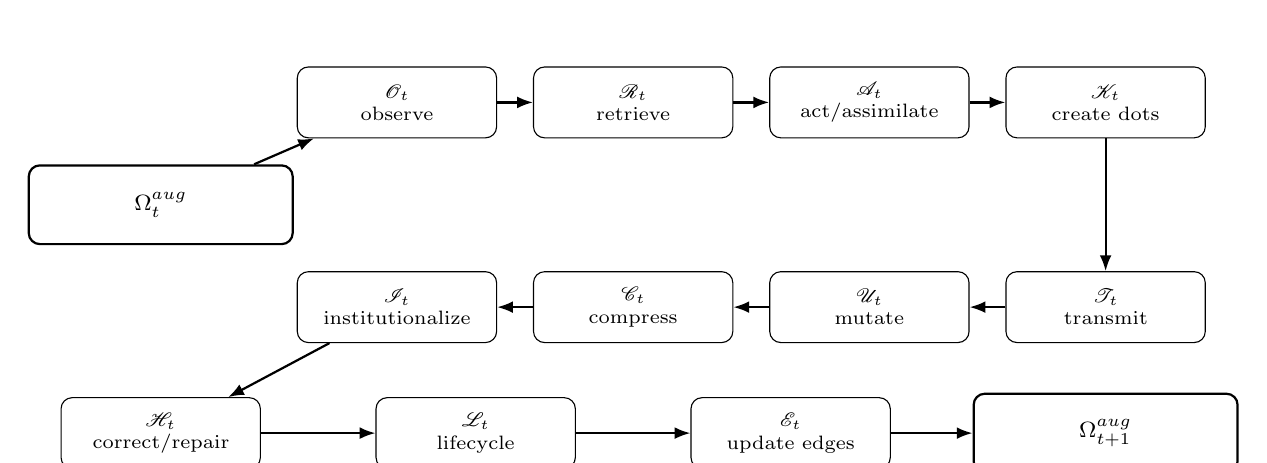
\begin{tikzpicture}[
  x=1cm,y=1cm,
  stage/.style={draw, rounded corners, align=center, text width=2.25cm, minimum height=0.9cm, font=\scriptsize, inner sep=4pt},
  state/.style={draw, rounded corners, thick, align=center, text width=3.0cm, minimum height=1.0cm, font=\footnotesize, inner sep=5pt},
  arr/.style={-{Latex[length=2mm]}, thick}
]
\node[state] (s0) at (0,0) {$\Omega_t^{aug}$};
\node[stage] (o) at (3.0,1.3) {$\mathscr O_t$\\observe};
\node[stage] (r) at (6.0,1.3) {$\mathscr R_t$\\retrieve};
\node[stage] (a) at (9.0,1.3) {$\mathscr A_t$\\act/assimilate};
\node[stage] (k) at (12.0,1.3) {$\mathscr K_t$\\create dots};
\node[stage] (tr) at (12.0,-1.3) {$\mathscr T_t$\\transmit};
\node[stage] (u) at (9.0,-1.3) {$\mathscr U_t$\\mutate};
\node[stage] (c) at (6.0,-1.3) {$\mathscr C_t$\\compress};
\node[stage] (i) at (3.0,-1.3) {$\mathscr I_t$\\institutionalize};
\node[stage] (h) at (0,-2.9) {$\mathscr H_t$\\correct/repair};
\node[stage] (l) at (4.0,-2.9) {$\mathscr L_t$\\lifecycle};
\node[stage] (e) at (8.0,-2.9) {$\mathscr E_t$\\update edges};
\node[state] (s1) at (12.0,-2.9) {$\Omega_{t+1}^{aug}$};
\draw[arr] (s0) -- (o); \draw[arr] (o) -- (r); \draw[arr] (r) -- (a); \draw[arr] (a) -- (k);
\draw[arr] (k) -- (tr); \draw[arr] (tr) -- (u); \draw[arr] (u) -- (c); \draw[arr] (c) -- (i);
\draw[arr] (i) -- (h); \draw[arr] (h) -- (l); \draw[arr] (l) -- (e); \draw[arr] (e) -- (s1);
\end{tikzpicture}%
}
\caption{Integrated mixed-mechanism transition. The diagram shows one canonical ordering for the augmented dot-field update. Alternative orderings are possible, but the ordering must be stated because transmission, mutation, correction, institutionalization, and topology update need not commute.}
\label{fig:integrated-dynamics}
\end{figure}


\begin{algorithmblock}{Canonical dot-field transition}
\label{alg:dot-field-transition}
\item \textbf{Input:} current augmented dot field $\Omega_t^{aug}$, environment $X_{t+1}$, active mechanism set $\mathcal G$, and stochastic or exogenous input $\varepsilon_{t+1}$.
\item \textbf{Output:} updated augmented dot field $\Omega_{t+1}^{aug}$ and audit log.
\item Observe the current environment, social graph, institutional stores, and available dot field.
\item Retrieve task-relevant dots for each acting agent using access, salience, credibility, recency, semantic relevance, and social proximity.
\item Select actions as functions of observations, internal state, goals, and retrieved dots.
\item Create new dots from action events, observations, claims, evaluations, records, and corrections.
\item Update access relations through social transmission, permissions, institutional publication, and private storage.
\item Apply mutation, compression, and institutionalization operators where the domain permits retelling, summarization, anchoring, or archival encoding.
\item Apply counter-dot and repair mechanisms to contested, false, obsolete, or reputationally damaging dots.
\item Update dot weights, credibility, salience, lifecycle status, and dot-dot relations.
\item Update social edges using dot-induced pressure, similarity, trust, reputation, obligation, or exclusion rules.
\item Return the updated augmented dot field $\Omega_{t+1}^{aug}$ and audit log.
\end{algorithmblock}


\subsection{Mechanism interfaces}\label{mechanism-interfaces}

Each mechanism is an operator on a state space. The operator may be deterministic, stochastic, or controlled by exogenous input. For the augmented dot field,
\[
\Omega_t^{aug}=(A,E_t,X_t,\bar S_t,D_t,R_t^D,B_t,\mathbf M_t,Q_t,L_t,I_t,C_t),
\]
the principal mechanism interfaces are as follows.

{\small
\begin{longtable}{@{}L{0.16\linewidth}L{0.25\linewidth}L{0.32\linewidth}L{0.12\linewidth}@{}}
\caption{Mechanism interfaces in the integrated dot-field transition.}\label{tab:mixed-mechanism-interfaces}\\
\toprule
\textbf{Operator} & \textbf{Primary input} & \textbf{Primary output} & \textbf{State level}\\
\midrule
\endfirsthead
\toprule
\textbf{Operator} & \textbf{Primary input} & \textbf{Primary output} & \textbf{State level}\\
\midrule
\endhead
\(\mathscr O_t\) observation & \(X_t,E_t,B_t,D_t\) & observations \(o_i(t)\) & core/aug\\
\(\mathscr R_t\) retrieval & \(\mathcal M_i(t),Q_t,R_t^D,q_i(t)\) & retrieved sets \(\mathcal V_i(q_i,t)\) & aug\\
\(\mathscr A_t\) action-assimilation & \(o_i(t),\mathcal V_i(q_i,t),\bar S_t\) & actions \(U_t\), updated internal states & aug\\
\(\mathscr K_t\) dot creation & \(U_t,X_t,\bar S_t\) & new dots \(D_t^{new}\) & core\\
\(\mathscr T_t\) transmission & \(E_t,B_t,Q_t,D_t\) & new access relations and descendants & aug\\
\(\mathscr U_t\) mutation & \(D_t,L_t,\varepsilon_t\) & mutated contents and updated lineage & aug\\
\(\mathscr C_t\) compression & finite dot subsets, retrieval history & compressed or reflective dots & aug\\
\(\mathscr I_t\) institutionalization & selected dots and artifacts & institutional dots and archives \(I_t\) & aug\\
\(\mathscr H_t\) correction-repair & counter-dots, target dots, \(C_t,Q_t\) & updated error margins and repair dots & aug\\
\(\mathscr L_t\) lifecycle update & usage, decay, reinforcement & updated \(\mathbf M_t,Q_t\), statuses & aug\\
\(\mathscr E_t\) topology update & retrieved evaluative dots and actions & updated social edges \(E_{t+1}\) & core/aug\\
\bottomrule
\end{longtable}
}

This table clarifies that mechanisms are not interchangeable. Retrieval requires accessible dots and effective strength. Mutation requires a lineage representation. Correction requires target dots and counter-dot fit. Institutionalization requires an institutional store. A dataset or simulator that lacks one of these state blocks should not claim to test the corresponding mechanism directly.

\subsection{Canonical mixed transition}\label{canonical-mixed-transition}

A canonical chronological ordering is:
\[
\Omega_{t+1}^{aug}=\mathscr F_t(\Omega_t^{aug},X_{t+1},\varepsilon_{t+1})
\]
with
\[
\mathscr F_t
=
\mathscr E_t\circ
\mathscr L_t\circ
\mathscr H_t\circ
\mathscr I_t\circ
\mathscr C_t\circ
\mathscr U_t\circ
\mathscr T_t\circ
\mathscr K_t\circ
\mathscr A_t\circ
\mathscr R_t\circ
\mathscr O_t.
\]
The order should be read as a default modeling convention, not as a universal sociological law. It says that agents first observe and retrieve, then act and assimilate, then new dots are created, transmitted, mutated, compressed, institutionalized, corrected, updated through lifecycle rules, and finally social edges are updated. Other domains may require a different order. For example, a public correction may occur before a platform transmits the original dot further, or an institutional record may be created before agents personally assimilate it.

The theory therefore distinguishes two kinds of order. \emph{Event order} is the temporal order observed in the domain. \emph{update order} is the computational order used by the model. A model is coherent only if the update order is either faithful to the event order or explicitly justified as an approximation.

\begin{definition}[Mixed dot-field process]
A mixed dot-field process is a stochastic process \(\{\Omega_t^{aug}\}_{t\geq 0}\) on augmented dot fields such that there exists a family of mechanism operators \(\mathscr F_t\) satisfying
\[
P(\Omega_{t+1}^{aug}\in C\mid \mathcal H_t)=K_t(C\mid \Omega_t^{aug})
\]
for measurable sets \(C\), whenever \(\Omega_t^{aug}\) is dot-state complete for the modeled process. The kernel \(K_t\) is induced by the composition of active mechanisms and exogenous randomness.
\end{definition}

\begin{definition}[Mechanism activation vector]
For a model instance, define the mechanism activation vector
\[
\mathbf a_t=(a_R,a_A,a_K,a_T,a_U,a_C,a_I,a_H,a_L,a_E)\in\{0,1\}^{10},
\]
where each coordinate indicates whether the corresponding mechanism is active at time \(t\). The core model has active retrieval, action-assimilation, dot creation, access update or transmission, lifecycle update, and topology update. Extensions activate mutation, compression, institutionalization, and correction as needed.
\end{definition}

The activation vector is useful for both theory and validation. A claim about semantic drift requires \(a_U=1\). A claim about institutional persistence requires \(a_I=1\). A claim about correction requires \(a_H=1\). If a mechanism is inactive in the model or unobservable in the data, the corresponding theorem should not be interpreted as tested.

\subsection{Well-definedness of the composed transition}\label{well-defined-composed-transition}

\begin{theorem}[Well-defined mixed dot-field dynamics]\label{thm:well-defined-mixed-dot-field-dynamics}
Let \((\mathcal X_\Omega,\mathcal B_\Omega)\) be the measurable state space of augmented dot fields. Suppose each active mechanism operator \(\mathscr G_s\) is a measurable transition kernel from valid augmented dot fields to valid augmented dot fields, possibly conditional on exogenous input and random seed. Then any finite composition
\[
\mathscr F_t=\mathscr G_{r,t}\circ\cdots\circ\mathscr G_{2,t}\circ\mathscr G_{1,t}
\]
defines a measurable transition kernel on \((\mathcal X_\Omega,\mathcal B_\Omega)\). If each \(\mathscr G_{s,t}\) preserves dot-field validity, then \(\mathscr F_t\) also preserves dot-field validity.
\end{theorem}

\begin{proof}
Measurability is closed under finite composition of measurable kernels. Validity preservation follows by induction. The first operator maps a valid state to a valid state by assumption. If the composition through step \(s-1\) maps valid states to valid states, then applying \(\mathscr G_{s,t}\) again produces a valid state. Hence all finite prefixes preserve validity, and the full composition preserves validity. The resulting map therefore induces a well-defined transition kernel over augmented dot fields.
\end{proof}

The theorem is intentionally modest. It does not prove convergence, truth, accuracy, or social benefit. It proves that once mechanism interfaces and validity conditions are specified, the combined model is a legitimate stochastic process rather than a loose list of mechanisms.

\subsection{Contractive mixed dynamics}\label{contractive-mixed-dynamics}

The next question is stability. Let \(d_\Omega\) be a product metric on augmented dot fields. It may combine distances over edge weights, access relations, dot weights, semantic embeddings, correction states, and institutional stores. For deterministic operators, say that \(\mathscr G_s\) is \(L_s\)-Lipschitz if
\[
d_\Omega(\mathscr G_s(\Omega),\mathscr G_s(\Omega'))\leq L_s d_\Omega(\Omega,\Omega')
\]
for all valid states \(\Omega,\Omega'\).

\begin{proposition}[Mixed-mechanism Lipschitz bound]
If active mechanism operators \(\mathscr G_1,\ldots,\mathscr G_r\) are Lipschitz with constants \(L_1,\ldots,L_r\), then the composed transition
\[
\mathscr F=\mathscr G_r\circ\cdots\circ\mathscr G_1
\]
is Lipschitz with constant
\[
L_{comp}\leq\prod_{s=1}^r L_s.
\]
\end{proposition}

\begin{proof}
Apply the Lipschitz inequality successively:
\[
d_\Omega(\mathscr G_r\cdots\mathscr G_1(\Omega),\mathscr G_r\cdots\mathscr G_1(\Omega'))
\leq L_r d_\Omega(\mathscr G_{r-1}\cdots\mathscr G_1(\Omega),\mathscr G_{r-1}\cdots\mathscr G_1(\Omega')),
\]
and iterate backward through \(\mathscr G_{r-1},\ldots,\mathscr G_1\). Multiplying the constants gives the bound.
\end{proof}

\begin{corollary}[Contraction condition]
If \((\mathcal X_\Omega,d_\Omega)\) is complete, \(\mathscr F\) is time-homogeneous, and
\[
\prod_{s=1}^r L_s<1,
\]
then \(\mathscr F\) is a contraction. It has a unique fixed point and repeated application converges to that fixed point from any initial augmented dot field in the invariant domain.
\end{corollary}

\begin{remark}[Interpretation]
The product condition is sufficient, not necessary. It gives a conservative stability criterion. If retrieval amplifies salient dots, transmission amplifies popularity, institutionalization increases authority, and topology feedback increases exposure, then several operators may have constants greater than one on relevant coordinates. In that case, the model can produce cascades, polarization, institutional lock-in, or reputation collapse rather than convergence.
\end{remark}

For stochastic operators, the same idea can be stated using Wasserstein contraction. If each mechanism kernel contracts expected distance by \(L_s\), then the composed kernel contracts by at most \(\prod_s L_s\). This formulation is useful for simulators and probabilistic agent models.

\subsection{Mechanism coupling regimes}\label{mechanism-coupling-regimes}

Mixed mechanisms can interact in at least four regimes.

\begin{description}[leftmargin=3.8cm,style=nextline]
\item[Independent regime]
Mechanisms act on separable state coordinates. For example, private memory decay may not affect institutional access. Order effects are weak or absent.

\item[Sequential regime]
One mechanism supplies input to another. Retrieval supplies action context; action supplies events; events create dots; created dots update access.

\item[Recursive regime]
Mechanisms feed back into one another. Social edges determine dot exposure, exposure changes retrieval, retrieval changes edge pressure, and edge pressure changes social edges.

\item[Adversarial or contested regime]
Mechanisms push in opposing directions. Institutionalization stabilizes a target dot while counter-dots attempt correction; mutation creates drift while anchoring attempts semantic stabilization.
\end{description}

These regimes guide theorem selection. Consensus results are most natural in independent or sequential regimes. Fragmentation, misinformation, and reputation cascades usually require recursive or contested regimes.

\subsection{Order dependence among mechanisms}\label{mechanism-order-dependence}

The temporal sequencing theorem showed that dot assimilation operators may be non-commutative. The same point applies to mechanisms. In general,
\[
\mathscr G_b\circ\mathscr G_a\neq \mathscr G_a\circ\mathscr G_b.
\]

\begin{proposition}[Mechanism-order sensitivity]
If two active mechanisms \(\mathscr G_a\) and \(\mathscr G_b\) fail to commute at a valid state \(\Omega\), meaning
\[
\mathscr G_b(\mathscr G_a(\Omega))\neq \mathscr G_a(\mathscr G_b(\Omega)),
\]
then there exists a mixed-process specification with the same active mechanisms and the same initial state but different update order that produces different next dot fields.
\end{proposition}

\begin{proof}
Construct two model specifications that are identical except for the order of \(\mathscr G_a\) and \(\mathscr G_b\). By the non-commutation condition, applying \(\mathscr G_a\) then \(\mathscr G_b\) yields a different state from applying \(\mathscr G_b\) then \(\mathscr G_a\). Thus update order changes the next dot field.
\end{proof}

Important non-commuting pairs include:
\[
\mathscr I\circ\mathscr H\neq \mathscr H\circ\mathscr I,
\]
because correcting a dot before institutionalization differs from correcting it after it has acquired institutional authority;
\[
\mathscr T\circ\mathscr U\neq \mathscr U\circ\mathscr T,
\]
because transmitting a dot before mutation can spread the original version, while mutating before transmission spreads the altered version; and
\[
\mathscr E\circ\mathscr B\neq \mathscr B\circ\mathscr E,
\]
because changing topology before access update can expose different agents than updating access before topology changes.

\subsection{Integrated topology-access-memory feedback}\label{integrated-topology-access-memory-feedback}

The most important mixed subsystem is the feedback loop among access, retrieval, and topology. A minimal recursive form is
\[
B_{t+1}=\mathscr B(E_t,D_t,Q_t,\varepsilon^B_t),
\]
\[
\mathcal V_i(q,t)=\mathscr R_i(B_t,D_t,Q_t,R_t^D,q_i),
\]
\[
\zeta_{ij}(t)=\mathscr P_{ij}(\mathcal V_i(q_{ij},t),Q_t),
\]
\[
E_{t+1}=\mathscr E(E_t,\boldsymbol{\zeta}_t,\varepsilon^E_t).
\]
This subsystem formalizes the claim that social ties shape trace exposure, trace exposure shapes retrieval, retrieval creates edge pressure, and edge pressure reshapes social ties.

\begin{proposition}[Feedback amplification condition]
Consider a scalar linearized feedback approximation around a local equilibrium:
\[
\Delta B_{t+1}=b_E\Delta E_t,
\]
\[
\Delta \zeta_t=\zeta_B\Delta B_t,
\]
\[
\Delta E_{t+1}=e_\zeta\Delta \zeta_t.
\]
The one-cycle feedback gain is
\[
G=b_E\zeta_Be_\zeta.
\]
If \(|G|<1\), small perturbations decay locally. If \(|G|>1\), small perturbations are locally amplified in the linear approximation.
\end{proposition}

\begin{proof}
Combining the three equations gives
\[
\Delta E_{t+1}=e_\zeta\zeta_Bb_E\Delta E_{t-1}=G\Delta E_{t-1}.
\]
Iterating yields geometric decay when \(|G|<1\) and geometric amplification when \(|G|>1\) within the validity range of the local linear approximation.
\end{proof}

This proposition is a bridge between topology feedback and fragmentation. If favorable dots increase edges, stronger edges increase exposure to the same favorable dots, and exposure increases favorable retrieval, then positive feedback can create alliance lock-in. If unfavorable dots reduce edges, weaker edges reduce counter-dot exposure, and reduced counter-dot exposure preserves unfavorable retrieval, then negative feedback can create exclusion or durable distrust.

\subsection{Failure modes of mixed dynamics}\label{mixed-dynamics-failure-modes}

The integrated model clarifies failure modes that are invisible when mechanisms are studied separately.

\begin{enumerate}[leftmargin=*]
\item \textbf{Amplification failure:} retrieval, transmission, and topology feedback jointly amplify a dot beyond its evidential support.
\item \textbf{Correction timing failure:} a counter-dot arrives after institutionalization, compression, or topology damage has already increased correction cost.
\item \textbf{Semantic mismatch failure:} mutation changes the public version of a target dot so that the available correction no longer semantically fits it.
\item \textbf{Access bottleneck failure:} bridge agents or institutional permissions block counter-dots from reaching affected components.
\item \textbf{Summary dominance failure:} compressed dots become more retrievable than their source details and drive action even when the source set is mixed.
\item \textbf{Measurement mismatch failure:} an empirical study observes communications but not access, retrieval, credibility, or correction reach, and therefore overstates the tested mechanism.
\end{enumerate}

\subsection{Reduced integrated model}\label{minimal-integrated-model}

For the base formal analysis, the canonical model is not the full extended model. It is the smallest mixed model that expresses the theory's central loop:
\[
\Omega_{t+1}^{min}=\mathscr E_t\circ\mathscr L_t\circ\mathscr B_t\circ\mathscr K_t\circ\mathscr A_t\circ\mathscr R_t\circ\mathscr O_t(\Omega_t^{core},\varepsilon_{t+1}).
\]
This model contains observation, retrieval, action-assimilation, dot creation, access update, lifecycle update, and topology update. Mutation, compression, institutionalization, and correction are extensions:
\[
\Omega_{t+1}^{full}=\mathscr E_t\circ\mathscr L_t\circ\mathscr H_t\circ\mathscr I_t\circ\mathscr C_t\circ\mathscr U_t\circ\mathscr T_t\circ\mathscr K_t\circ\mathscr A_t\circ\mathscr R_t\circ\mathscr O_t(\Omega_t^{aug},\varepsilon_{t+1}).
\]
The reduced model supports the cleanest representation claim because it contains only observation, retrieval, action-assimilation, dot creation, access update, lifecycle update, and topology update. The full model is required when the application involves rumors, archives, summaries, corrections, semantic drift, reputation repair, or institutional governance. Distinguishing these two levels helps keep the theory modular: a study need not activate every mechanism, but it should state which operators are active and which omitted mechanisms are outside the claim.

\subsection{Integrated contribution}\label{integrated-contribution}

The integrated dynamics section turns the theory from a collection of dot mechanisms into a unified state-transition framework. Its main contribution is not that every social system contains every mechanism. The contribution is that, when these mechanisms are present, they can be represented as typed operators acting on a common dot-field state. This yields three benefits:

\begin{enumerate}[leftmargin=*]
\item \textbf{Coherence:} retrieval, transmission, mutation, institutionalization, correction, and topology feedback are no longer separate vocabularies.
\item \textbf{Modularity:} mechanisms can be activated or deactivated without changing the underlying state hierarchy.
\item \textbf{Testability:} empirical and simulation claims can state exactly which operators are active, which state variables are observed, and which failure modes are possible.
\end{enumerate}

The later theorem sections are therefore best read as analyses of submodels of the mixed transition rather than as disconnected mathematical claims.


\section{Recursive Topology-Feedback Stability}\label{recursive-topology-feedback-stability}

The integrated mixed-mechanism section identifies the central recursive subsystem of Dot-Trace Theory: social edges influence dot access, access influences retrieval, retrieval produces edge pressure, and edge pressure changes social edges. A coherent dynamic theory therefore requires explicit stability conditions for this loop, rather than only a scalar feedback diagnostic.

This section studies that loop directly. The results are conditional stability results rather than universal convergence claims. They identify when recursive dot-topology feedback is contractive, when it amplifies perturbations, and when thresholded access can produce self-sealing exclusion or fragmented correction.



\begin{figure}[htbp]
\centering
\resizebox{0.92\textwidth}{!}{%
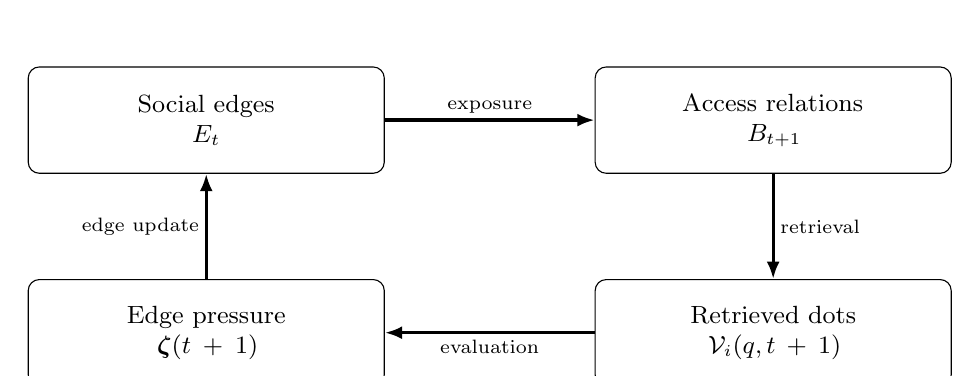
\begin{tikzpicture}[
  x=1cm,y=1cm,
  box/.style={draw, rounded corners, align=center, text width=4.1cm, minimum height=1.35cm, font=\small, inner sep=6pt},
  lab/.style={font=\scriptsize, fill=white, inner sep=2pt},
  arr/.style={-{Latex[length=2.2mm]}, very thick}
]
\node[box] (e) at (0,2.7) {Social edges\\$E_t$};
\node[box] (b) at (7.2,2.7) {Access relations\\$B_{t+1}$};
\node[box] (v) at (7.2,0) {Retrieved dots\\$\mathcal V_i(q,t+1)$};
\node[box] (z) at (0,0) {Edge pressure\\$\boldsymbol\zeta(t+1)$};
\draw[arr] (e) -- node[lab, above] {exposure} (b);
\draw[arr] (b) -- node[lab, right] {retrieval} (v);
\draw[arr] (v) -- node[lab, below] {evaluation} (z);
\draw[arr] (z) -- node[lab, left] {edge update} (e);
\end{tikzpicture}%
}
\caption{Recursive topology-access-memory feedback. Social edges shape dot access; access shapes retrieval; retrieval produces edge pressure; edge pressure changes social edges. Stability depends on the gain around this loop.}
\label{fig:recursive-feedback-loop}
\end{figure}



\subsection{Feedback subsystem and reduced edge map}\label{feedback-subsystem-reduced-edge-map}

For analysis, let
\[
e_t=\operatorname{vec}(E_t)\in \mathcal E\subseteq [0,1]^p
\]
be the vector of relevant social edge weights. Let
\[
b_t=\operatorname{vec}(B_t)\in \mathcal B\subseteq [0,1]^q
\]
be a soft access vector, where entries may represent probabilities, intensities, permissions, or exposure propensities rather than only binary access. Let
\[
r_t\in\mathcal R
\]
summarize retrieved-dot features, and let
\[
\zeta_t\in\mathcal Z\subseteq \mathbb R^p
\]
represent edge pressure induced by retrieved evaluative dots.

A recursive topology-access-memory subsystem has the form
\[
b_{t+1}=F_B(e_t,\Xi_t,\xi^B_{t+1}),
\]
\[
r_{t+1}=F_R(b_{t+1},\Xi_t,\xi^R_{t+1}),
\]
\[
\zeta_{t+1}=F_\zeta(r_{t+1},\Xi_t,\xi^\zeta_{t+1}),
\]
\[
e_{t+1}=F_E(e_t,\zeta_{t+1},\Xi_t,\xi^E_{t+1}),
\]
where
\[
\Xi_t=(D_t,R_t^D,\mathbf M_t,Q_t,L_t,I_t,C_t,X_t)
\]
collects the non-edge dot-field background during the feedback step.

When \(\Xi_t\) is fixed or slowly varying over the phase of interest and the maps are deterministic, the edge dynamics reduce to a composite map
\[
e_{t+1}=\Theta(e_t),
\]
where
\[
\Theta(e)=F_E\big(e,F_\zeta(F_R(F_B(e,\Xi),\Xi),\Xi),\Xi\big).
\]
This is the reduced recursive edge map. It does not remove dots from the theory. Rather, it compresses the dot-mediated feedback loop into an edge map after conditioning on a fixed dot-field background.

\begin{definition}[Recursive topology-feedback loop]
A topology-feedback loop is recursive when the social edge state \(e_t\) affects future dot access or retrieval and the resulting retrieved-dot pressure affects \(e_{t+1}\). It is nonrecursive when edge pressure is exogenous to the topology or when access and retrieval do not depend on current social edges.
\end{definition}

\begin{definition}[Stability of a dot-topology equilibrium]
A state \(e^\star\) is a stable dot-topology equilibrium for a fixed dot-field background \(\Xi\) if \(\Theta(e^\star)=e^\star\) and all sufficiently small perturbations of \(e^\star\) remain near \(e^\star\) under repeated application of \(\Theta\). It is asymptotically stable if those perturbations converge back to \(e^\star\).
\end{definition}

The fixed-background assumption is not a claim that dots never change. It is a phase assumption, analogous to the fixed-vocabulary assumptions used in the consensus theorem. It is appropriate for studying short-run stability, local cascades, and feedback around a slowly changing dot field. Longer horizons require the full mixed transition of Section~\ref{integrated-mixed-mechanism-dynamics}.

\subsection{Global contraction condition}\label{global-contraction-condition}

The most conservative stability result uses Lipschitz bounds. Suppose that, for a fixed background \(\Xi\), the access, retrieval, and pressure maps satisfy
\[
\|F_B(e,\Xi)-F_B(e',\Xi)\|\leq L_B\|e-e'\|,
\]
\[
\|F_R(b,\Xi)-F_R(b',\Xi)\|\leq L_R\|b-b'\|,
\]
\[
\|F_\zeta(r,\Xi)-F_\zeta(r',\Xi)\|\leq L_\zeta\|r-r'\|.
\]
Assume also that the edge-update map satisfies
\[
\|F_E(e,z,\Xi)-F_E(e',z',\Xi)\|\leq L_E^e\|e-e'\|+L_E^\zeta\|z-z'\|.
\]

\begin{theorem}[Recursive feedback contraction]\label{thm:recursive-feedback-contraction}
Under the Lipschitz assumptions above, the reduced recursive edge map \(\Theta\) satisfies
\[
\|\Theta(e)-\Theta(e')\|\leq
\left(L_E^e+L_E^\zeta L_\zeta L_R L_B\right)\|e-e'\|.
\]
If
\[
L_E^e+L_E^\zeta L_\zeta L_R L_B<1,
\]
then \(\Theta\) is a contraction. On a complete invariant edge domain, \(\Theta\) has a unique fixed point, and repeated topology-feedback updates converge to it from any initial edge state in that domain.
\end{theorem}

\begin{proof}
For any two edge states \(e,e'\), the access map gives
\[
\|F_B(e)-F_B(e')\|\leq L_B\|e-e'\|.
\]
Applying the retrieval map gives
\[
\|F_R(F_B(e))-F_R(F_B(e'))\|\leq L_R L_B\|e-e'\|.
\]
Applying the pressure map gives
\[
\|F_\zeta F_R F_B(e)-F_\zeta F_R F_B(e')\|\leq L_\zeta L_R L_B\|e-e'\|.
\]
The edge update then yields
\[
\|\Theta(e)-\Theta(e')\|
\leq L_E^e\|e-e'\|+L_E^\zeta L_\zeta L_R L_B\|e-e'\|.
\]
This proves the Lipschitz bound. If the coefficient is below one, the Banach fixed-point argument gives uniqueness and convergence on the complete invariant domain.
\end{proof}

A common edge update is a convex-inertia rule
\[
e_{t+1}=(1-\eta)e_t+\eta\phi(\zeta_{t+1}),\qquad 0<\eta\leq 1,
\]
where \(\phi\) maps edge pressure into target edge weights. If \(\phi\) is \(L_\phi\)-Lipschitz, then
\[
L_E^e=1-\eta,\qquad L_E^\zeta=\eta L_\phi.
\]
The contraction condition becomes
\[
(1-\eta)+\eta L_\phi L_\zeta L_R L_B<1,
\]
or equivalently
\[
L_\phi L_\zeta L_R L_B<1.
\]
Thus inertia alone does not guarantee stability. The dot-mediated feedback gain from edges to access, access to retrieval, retrieval to pressure, and pressure back to edges must also remain below the amplifying threshold.

\subsection{Local Jacobian stability}\label{local-jacobian-stability}

The global contraction condition is strong. Local stability can be studied by differentiating the feedback loop around an equilibrium. Suppose the maps are differentiable near a fixed point \(e^\star\). Let
\[
B_e=D_eF_B(e^\star),\qquad R_b=D_bF_R(b^\star),\qquad \zeta_r=D_rF_\zeta(r^\star),
\]
\[
E_e=D_eF_E(e^\star,\zeta^\star),\qquad E_\zeta=D_\zeta F_E(e^\star,\zeta^\star).
\]
The Jacobian of the reduced edge map is
\[
J_\Theta=E_e+E_\zeta \zeta_r R_b B_e.
\]
The term \(E_e\) is direct edge inertia. The product \(E_\zeta \zeta_r R_b B_e\) is the recursive dot-mediated feedback channel.

\begin{theorem}[Local stability of recursive topology feedback]\label{thm:local-stability-recursive-topology-feedback}
Let \(e^\star\) be a fixed point of \(\Theta\), and suppose \(\Theta\) is continuously differentiable in a neighborhood of \(e^\star\). If
\[
\rho(J_\Theta)<1,
\]
where \(\rho(\cdot)\) denotes spectral radius, then \(e^\star\) is locally asymptotically stable. If \(\rho(J_\Theta)>1\), then there exist arbitrarily small perturbations whose linearized first-order dynamics are amplified away from \(e^\star\).
\end{theorem}

\begin{proof}
Let \(u_t=e_t-e^\star\). A first-order expansion gives
\[
u_{t+1}=J_\Theta u_t+o(\|u_t\|).
\]
If \(\rho(J_\Theta)<1\), then there exists a compatible norm in which \(J_\Theta\) has operator norm below one. The nonlinear remainder is of smaller order near the fixed point, so sufficiently small perturbations contract and converge to zero. If \(\rho(J_\Theta)>1\), the linear map has an expanding eigendirection or generalized expanding direction. Along sufficiently small perturbations in that direction, the first-order term dominates the higher-order remainder initially, producing local amplification in the linearized approximation.
\end{proof}

The theorem gives a more precise version of the earlier scalar feedback gain. In one dimension,
\[
J_\Theta=E_e+E_\zeta \zeta_r R_b B_e,
\]
and stability requires
\[
|E_e+E_\zeta \zeta_r R_b B_e|<1.
\]
The scalar gain is therefore only the feedback-channel term. The full local stability condition also includes direct edge inertia.

\subsection{Feedback sign regimes}\label{feedback-sign-regimes}

The sign of the recursive product matters. Let
\[
\mathcal G=E_\zeta \zeta_r R_b B_e
\]
be the local dot-mediated feedback channel.

\begin{description}[leftmargin=4cm,style=nextline]
\item[Reinforcing feedback]
When \(\mathcal G\) has positive dominant effect, stronger edges increase exposure to dots that further strengthen those edges, or weaker edges reduce exposure to counter-dots that could repair the edge. This regime supports lock-in, alliance formation, reputation cascades, and exclusion.

\item[Balancing feedback]
When \(\mathcal G\) has negative dominant effect, stronger edges increase exposure to corrective or diversifying dots that reduce edge pressure, or weaker edges increase search for repair. This regime can stabilize the system but may oscillate if the magnitude is large.

\item[Broken feedback]
When at least one channel has near-zero sensitivity, topology does not recursively amplify dot exposure. Edge updates may still occur, but they behave more like exogenous-pressure updates than feedback dynamics.
\end{description}

This sign distinction is important for social capital. Bonding capital can be stabilizing when it increases reliable correction within a group, but amplifying when it increases repeated exposure to only internally reinforcing dots. Bridging capital can be stabilizing when it supplies counter-dots across communities, but destabilizing when bridges transmit high-salience false dots before correction is available.

\subsection{Threshold closure and self-sealing exclusion}\label{threshold-closure-self-sealing-exclusion}

Many social systems are not smooth. Access often changes discontinuously: a person is blocked, a channel is closed, a permission is revoked, a group chat removes a member, or an institution restricts a record. Threshold access can make feedback self-sealing.

Consider a single directed relation \(w_t\in[0,1]\). Suppose an important counter-dot is accessible only when
\[
w_t\geq \tau_B.
\]
When the counter-dot is inaccessible, the edge target is \(\theta_0\), with
\[
0\leq \theta_0<\tau_B.
\]
The edge update is
\[
w_{t+1}=(1-\eta)w_t+\eta\theta_0,
\qquad 0<\eta\leq 1,
\]
for as long as \(w_t<\tau_B\).

\begin{proposition}[Threshold access closure]
If \(w_t<\tau_B\) and the inaccessible-counter-dot regime has target \(\theta_0<\tau_B\), then
\[
w_{t+k}<\tau_B
\]
for every \(k\geq 1\), and
\[
w_{t+k}\to \theta_0.
\]
Thus once the edge falls below the access threshold, the relation remains closed unless an external intervention or alternative access path changes the target.
\end{proposition}

\begin{proof}
Both \(w_t\) and \(\theta_0\) are below \(\tau_B\). Their convex combination is therefore below \(\tau_B\):
\[
w_{t+1}=(1-\eta)w_t+\eta\theta_0<\tau_B.
\]
The same argument applies inductively. The recursion is linear, so
\[
w_{t+k}=\theta_0+(1-\eta)^k(w_t-\theta_0),
\]
which converges to \(\theta_0\).
\end{proof}

This proposition formalizes a common social-memory failure mode. A negative dot weakens an edge. The weakened edge removes access to the counter-dot. Without counter-dot access, the negative pressure remains uncorrected. The damaged edge then stabilizes below the threshold. In social terms, distrust can become self-sealing because the channel through which correction would arrive has been closed.

\subsection{Bridge recovery and correction reach}\label{bridge-recovery-correction-reach}

The opposite result describes when a bridge or institutional channel can reopen a relation. Suppose an external bridge, archive, mediator, or platform gives the agent enough counter-dot exposure to make the edge target \(\theta_1\), where
\[
\theta_1>\tau_B.
\]
The edge update becomes
\[
w_{t+1}=(1-\eta)w_t+\eta\theta_1.
\]

\begin{proposition}[Finite-time bridge recovery]
If \(w_t<\tau_B<\theta_1\), then the edge crosses the access threshold after finite time. In particular, any integer \(k\) satisfying
\[
(1-\eta)^k<\frac{\theta_1-\tau_B}{\theta_1-w_t}
\]
ensures
\[
w_{t+k}>\tau_B.
\]
\end{proposition}

\begin{proof}
The solution of the recursion is
\[
w_{t+k}=\theta_1+(1-\eta)^k(w_t-\theta_1).
\]
The condition \(w_{t+k}>\tau_B\) is equivalent to
\[
\theta_1-(1-\eta)^k(\theta_1-w_t)>\tau_B,
\]
which rearranges to the stated inequality.
\end{proof}

This result connects recursive stability to correction and social capital. Bridge agents, archives, mediators, and institutional records matter because they can maintain correction reach even after ordinary social edges fall below access thresholds. Their value is not only that they connect components; it is that they can prevent topology from making counter-evidence unreachable.

\subsection{Stability, fragmentation, and social capital}\label{stability-fragmentation-social-capital}

Recursive topology feedback sharpens the relation between dot theory and social capital. An agent's social capital depends not only on the number or strength of its ties, but also on whether those ties provide stabilizing or destabilizing trace exposure.

For a group \(G\), define a local recursive stability margin
\[
SM_G(t)=1-\rho(J_{\Theta,G}(t)),
\]
where \(J_{\Theta,G}(t)\) is the Jacobian or empirical linearization of the feedback loop restricted to group-relevant edges. Positive margin indicates local damping. Negative margin indicates local amplification.

Define access-closure risk for relation \((i,j)\) as
\[
ACR_{ij}(t)=\mathbf 1\{w_{ij}(t)<\tau_B,\ \theta_{ij}^{closed}(t)<\tau_B\}.
\]
Define bridge recovery margin as
\[
BRM_{ij}(t)=\theta_{ij}^{bridge}(t)-\tau_B.
\]
A positive bridge recovery margin means that available bridge or institutional correction is strong enough, if sustained, to reopen the access channel.

These quantities refine the social-capital decomposition. Bonding capital without bridge recovery can deepen internal convergence while increasing external closure. Bridging capital has high value when it increases \(BRM\) or reduces \(ACR\). Correction capital has high value when it lowers the dominance of \(\theta^{closed}\) or raises \(\theta^{bridge}\) above the access threshold.

\subsection{Measurement implications}\label{recursive-stability-measurement-implications}

Testing recursive topology-feedback stability requires more than observing social edges. At minimum, a study must observe or estimate:

\begin{enumerate}[leftmargin=*]
\item edge changes over time;
\item which dots or dot classes become accessible as edges change;
\item which accessible dots are retrieved or used in edge-relevant decisions;
\item edge pressure induced by retrieved evaluative dots;
\item whether counter-dots remain reachable after edge weakening.
\end{enumerate}

Edge-only data may identify that a tie decayed, but not whether it decayed because of recursive dot exposure, unobserved external events, institutional access changes, or unrelated preference drift. For this reason, recursive stability claims generally require O3--O5 observability or a simulator in which access and retrieval are controlled.

\subsection{Contribution of the stability layer}\label{contribution-stability-layer}

The recursive stability layer completes the core dynamic picture. The representational theorems explain why dots must be included. The mixed-mechanism section explains how dot processes compose. The stability results explain when the central feedback loop converges, amplifies, closes access, or recovers through bridges. This moves the theory from ``dots affect edges'' to a more precise claim:

\begin{quote}
In memory-sensitive social systems, topology and trace exposure can form a recursive dynamical loop. Stability depends on the sensitivity of access to edges, retrieval to access, edge pressure to retrieval, and edge update to pressure.
\end{quote}

This loop is the formal core of dot-mediated echo chambers, reputation cascades, durable distrust, bridge-based recovery, and topology-mediated social capital.


\section{Worked Examples and Boundary Cases}\label{worked-examples-boundary-cases}

The formal sections above define the dot field, mixed-mechanism transition, and recursive topology-feedback loop. This section shows how the same machinery operates in concrete cases. The examples are not empirical evidence. They are worked instantiations: each identifies agents, dots, access relations, retrieval, topology feedback, and expected theorem signatures.

\subsection{Example 1: Two-agent trust repair after betrayal}\label{example-two-agent-trust-repair}

Let two agents be
\[
A=\{a_i,a_j\}.
\]
At time $t_0$, agent $a_j$ defects in a joint task. The event creates an evaluative dot
\[
d^-=(\text{``}a_j \text{ defected against } a_i\text{''},T(d^-)=a_j,v_i(d^-,j)<0,\tau=t_0).
\]
If $a_i$ has access to $d^-$, then
\[
(a_i,d^-)\in B_{t_0+1}
\]
and $d^-$ may be retrieved in later decisions about whether to cooperate with $a_j$:
\[
d^-\in \mathcal V_i(q_{ij},t).
\]
The retrieved negative dot creates edge pressure
\[
\zeta_{ij}(t)=\sum_{d\in \mathcal V_i(q_{ij},t):T(d)=a_j}\omega_i(d,t)v_i(d,j,t)<0.
\]
A dot-responsive edge update then lowers trust:
\[
w_{ij}(t+1)=(1-\eta)w_{ij}(t)+\eta\psi(\zeta_{ij}(t)).
\]

Suppose $a_j$ later apologizes, compensates $a_i$, or completes a repair action. This creates a counter-dot or repair dot
\[
c^+=(\text{``}a_j repaired the harm\text{''},T(c^+)=a_j,v_i(c^+,j)>0),
\]
with relation
\[
c^+\dashv d^-.
\]
Correction succeeds only if the counter-dot has sufficient effective strength and fit:
\[
CE_i(c^+,d^-,t)=Q_i(c^+,t)\kappa_i(c^+,d^-,t).
\]
If correction pressure exceeds reinforcement load, the active error or liability margin associated with $d^-$ declines. Social repair, however, is not automatic. Even if the factual status of $d^-$ is corrected, the edge $w_{ij}$ may remain low unless the new positive pressure moves the edge target above a repair threshold.

This example instantiates representational insufficiency, counter-dot correction, residual topology harm, and bridge recovery. An agent-edge model that stores only the current value of $w_{ij}$ may predict the next interaction if that value is already dot-sufficient. But if two systems share the same current edge weight while one contains $d^-$ and the other contains $c^+\dashv d^-$, their future behavior may diverge. The dot field is then necessary.

\subsection{Example 2: Organizational incident memory}\label{example-organizational-incident-memory}

Consider a project team
\[
G=\{a_1,\ldots,a_n\}
\]
that experiences a failed deployment. The incident produces multiple dots:
\[
d_1=\text{``deployment failed at 02:13''},
\]
\[
d_2=\text{``rollback was delayed because approval was unclear''},
\]
\[
d_3=\text{``engineer }a_k\text{ issued the first alert''},
\]
\[
d_4=\text{``new approval rule adopted after incident''}.
\]
Some dots are private memories; others become institutional dots when encoded in a postmortem, ticket, or policy:
\[
\mathcal I_t(d_2)=d_2^I,\qquad \mathcal I_t(d_4)=d_4^I.
\]
Institutionalization changes persistence and reach. If $\lambda_I>\lambda_P$, then the institutional postmortem decays more slowly than private recollections. If many agents have access to the archive, then
\[
R^I(d_2,t)=\sum_i \mathbf 1\{(a_i,d_2^I)\in B_t^I\}
\]
may exceed the reach of private dots.

The same incident can also generate compression. Several technical details may be summarized into one higher-level dot:
\[
d^*=C(\{d_1,d_2,d_3,d_4\})=\text{``the failure was caused by unclear approval procedure''}.
\]
This summary may coordinate future behavior, but it can also erase detail. If the deployment actually failed because of two independent causes and $d^*$ hides one of them, then compression creates behavioral loss. A later team may retrieve the simplified institutional dot and improve approval rules while neglecting monitoring, staffing, or tool reliability.

This example instantiates institutional stabilization, compression insufficiency, summary dominance, and archival social capital. An agent with access to the postmortem may possess archival social capital because the archive improves future coordination. But if the archived summary is wrong, the same institutional dot can stabilize an error.

\subsection{Example 3: Bridge-mediated collective memory}\label{example-bridge-collective-memory}

Let two groups $C_1$ and $C_2$ discuss the same event but initially receive different dots. Group $C_1$ receives
\[
d_p=\text{``the policy reduced risk''},
\]
while group $C_2$ receives
\[
d_q=\text{``the policy created unfair costs''},
\]
with a contradiction relation
\[
d_p\dashv d_q.
\]
Within each component, repeated discussion updates dot weights through an influence matrix. If the components are disconnected, each may converge internally to a different memory barycenter:
\[
\bar m^{(1)}\neq \bar m^{(2)}.
\]
This is fragmented collective memory.

Now introduce a bridge agent $a_b$ with ties to both components. The bridge can transmit $d_p$, $d_q$, or a counter-dot $c$ before or after each component internally reinforces its own interpretation. If bridge transmission occurs early, the transmitted dot can be incorporated before local convergence. If it occurs late, it faces an already stabilized local dot field. Formally, if bridge injection $B_\varepsilon$ occurs before reinforcement $R_\alpha$, then
\[
R_\alpha(B_\varepsilon(0))>B_\varepsilon(R_\alpha(0))
\]
under the bridge-amplification conditions developed earlier.

This example instantiates consensus, fragmentation, bridge timing, non-commutativity, bonding capital, and bridging capital. The bridge agent's advantage is not merely structural degree. It lies in controlling when and how dots cross component boundaries. That is dot-mediated bridging capital.

\subsection{Example 4: Public accusation, correction, and residual harm}\label{example-public-accusation-correction}

Suppose a public platform contains agents $A$, posts, reposts, comments, and moderation records. A high-status agent publishes an accusation:
\[
d_A=\text{``}a_j\text{ committed misconduct''}.
\]
The accusation is evaluative, public, high-salience, and targeted:
\[
T(d_A)=a_j,\qquad v_i(d_A,j)<0.
\]
Because the source is high-status, many agents assign high credibility to the dot. The dot induces negative edge pressure toward $a_j$, lowering trust and increasing exclusion risk:
\[
ER_j^\tau(t)=\Pr\{w_{ij}(t)<\tau \text{ for many } i\}.
\]

Later, a correction appears:
\[
c_A=\text{``the accusation was based on a misidentified event''},\qquad c_A\dashv d_A.
\]
The correction's existence is not enough. It must reach agents who saw the accusation, be retrieved in relevant contexts, be credible, and semantically target the version of the accusation they hold. If the accusation mutated into a more general label such as
\[
d'_A=\text{``}a_j\text{ is unsafe''},
\]
then a narrow correction may have low semantic fit:
\[
\kappa_i(c_A,d'_A,t)=\exp(-\beta_i\Delta_{\mathcal X}(x(c_A),x(d'_A))).
\]

Even after factual correction, social repair may lag. The residual topology harm is
\[
RTH_j(t)=\sum_{i\neq j}[w_{ij}^{pre}-w_{ij}^{post}]_+.
\]
Repair requires not only a counter-dot but additional positive repair dots, bridge recovery, or institutional correction. This example shows why Dot-Trace Theory separates factual correction from topology repair.

\subsection{Example 5: LLM-agent workspace with public and private memory}\label{example-llm-agent-workspace}

Consider an artificial workplace populated by LLM-based agents. Agents interact through chat, task tools, shared documents, issue trackers, and private memories. A completed task creates dots such as
\[
d_1=\text{``}a_k\text{ completed the database migration''},
\]
\[
d_2=\text{``}a_l\text{ missed the review deadline''},
\]
\[
d_3=\text{``the migration checklist is now canonical''}.
\]
The public issue tracker creates institutional dots. Private agent memories create private dots. Agent retrieval determines planning and delegation. Repeated positive evaluative dots may increase reputation capital for $a_k$; repeated negative dots may increase liability for $a_l$.

The same setting can instantiate mutation and compression. A detailed technical dot may be summarized by an LLM into a shorter memory entry. If the summary omits a security caveat, then future agents may retrieve a compressed dot that changes behavior. If a shared checklist anchors the correct version, semantic drift can be reduced. If the checklist is wrong, anchoring stabilizes the wrong trace.

This example motivates implementation and validation. It has observable messages, access logs, documents, actions, and topology changes, making it a strong candidate for synthetic and eventually empirical dot-field benchmarking. It also shows why the theory distinguishes access, attention, retrieval, and action: an agent may have permission to view a document, never attend to it, retrieve the wrong summary, and act on that summary.

\subsection{Boundary case: when Dot-Trace Theory is unnecessary}\label{boundary-case-dot-theory-unnecessary}

A theory is more useful when it states its limits. Suppose agents interact in a fully observable, memoryless coordination game where all transition-relevant information is contained in
\[
Z_t=(A,E_t,X_t,\bar S_t),
\]
and no persistent trace affects future action except through variables already encoded in $Z_t$. Then
\[
I(Y_{t+1};D_t,R_t^D,B_t,\mathbf M_t,Q_t,L_t\mid Z_t)=0.
\]
In this case, the dot field may be descriptively interesting but predictively unnecessary. A dot-free model is sufficient for the specified outcome and horizon. This boundary case is important because it prevents the theory from becoming unfalsifiable. Dot-Trace Theory is needed only when trace-mediated information remains transition-relevant after conditioning on the reduced state. In empirical work, this boundary case corresponds to a genuine null result: if well-measured dot-field variables do not improve prediction, mechanism identification, or intervention reasoning beyond appropriate baselines, then the reduced representation is adequate for that domain.

\subsection{Worked-example synthesis}\label{worked-example-synthesis}

Table~\ref{tab:worked-example-synthesis} summarizes the examples in relation to the formal machinery.

{\small
\begin{longtable}{@{}L{0.17\textwidth}L{0.26\textwidth}L{0.26\textwidth}L{0.19\textwidth}@{}}
\caption{Worked examples mapped to dot-field mechanisms and theorem signatures.}\label{tab:worked-example-synthesis}\\
\toprule
\textbf{Example} & \textbf{Key dot-field objects} & \textbf{Active mechanisms} & \textbf{Theorem signatures}\\
\midrule
\endfirsthead
\toprule
\textbf{Example} & \textbf{Key dot-field objects} & \textbf{Active mechanisms} & \textbf{Theorem signatures}\\
\midrule
\endhead
Trust repair & Evaluative dot, counter-dot, repair dot, edge pressure. & Retrieval, correction, topology update, repair. & Insufficiency, correction threshold, residual topology harm.\\
Organizational incident & Institutional dots, compressed summary, archive access, provenance. & Institutionalization, compression, lifecycle, archival reach. & Institutional stabilization, compression loss, archival capital.\\
Bridge collective memory & Contradictory dots, bridge access, component barycenters. & Transmission, consensus, fragmentation, temporal sequencing. & Consensus, fragmented memory, bridge amplification.\\
Public accusation & High-salience negative dot, mutated accusation, correction, reputation edges. & Testimony, mutation, correction, exclusion, repair. & Dot-induced topology, semantic drift, correction mismatch.\\
LLM-agent workspace & Public documents, private memories, issue logs, agent retrieval traces. & Creation, retrieval, mutation, compression, institutional anchors. & Implementation, prediction lift, measurement ladder.\\
Memoryless boundary & No transition-relevant dot information beyond $Z_t$. & None required. & Zero projection loss; dot-free sufficiency.\\
\bottomrule
\end{longtable}
}

The examples also clarify the relation among dots, centroids, and social capital. A dot is not a centroid by definition. In the bridge example, however, a trace may become a group memory hub in the lifted heterogeneous graph. Social capital is not a dot either. In the organizational and public-accusation examples, social capital is a derived advantage or liability generated by access to useful, trusted, corrective, or reputational dots.

\section{Model Assumptions and Proof Obligations}\label{model-assumptions-proof-obligations}

A theory of social memory can easily become overbroad. Dot-Trace Theory
therefore separates its assumptions from its conclusions. The formal
results below are conditional theorems, not universal sociological laws.

\subsection{Minimal assumptions}\label{minimal-assumptions}

The baseline formal package assumes:

\begin{enumerate}[leftmargin=*]
\item \textbf{Memory sensitivity:} at least some agents condition action on retrieved traces.
\item \textbf{Persistence:} at least some traces persist across time steps.
\item \textbf{Partial access:} different agents may access different dot subsets.
\item \textbf{Transmission:} access can change through communication, publication, recommendation, or institutional storage.
\item \textbf{Lifecycle change:} dot strength, credibility, salience, and visibility may decay, reinforce, mutate, or be corrected.
\item \textbf{Topology feedback:} retrieved evaluative dots can affect trust, affinity, communication, exclusion, or alliance edges.
\end{enumerate}

If these assumptions fail, the theory may still provide a vocabulary,
but its strongest representation and prediction claims no longer follow.

\subsection{Levels of theoretical strength}\label{levels-theoretical-strength}

The claims in the article have different statuses:

\begin{longtable}{L{0.24\linewidth}L{0.68\linewidth}}
\toprule
\textbf{Claim type} & \textbf{Standard required}\\
\midrule
Definition & Internal coherence and usefulness across examples.\\
Axiom & Clear scope and plausibility for the target class of systems.\\
Theorem & Formal derivation from stated assumptions.\\
Simulation result & Reproducible behavior under specified parameters and ablations.\\
Empirical result & Held-out predictive, causal, or explanatory value against baselines and negative controls.\\
Ontological claim & Evidence that dot-field quantities are not merely relabelings of existing variables in the target context.\\
\bottomrule
\end{longtable}

This separation is important. A theorem can prove a conditional
representational fact without proving that a particular real-world
system satisfies the theorem's assumptions. Conversely, an empirical
prediction lift can support the usefulness of dot variables without
settling the full ontology of the dot field.

\subsection{Theorem dependency map}\label{theorem-dependency-map}

The theoretical results are organized as a dependency chain rather than
as isolated claims.

\begin{longtable}{L{0.22\linewidth}L{0.35\linewidth}L{0.35\linewidth}}
\toprule
\textbf{Result} & \textbf{Depends on} & \textbf{Provides}\\
\midrule
Representational insufficiency & Memory sensitivity and omitted dot state & Justification for adding dots to the state.\\
Markov restoration & Complete transition-relevant dot encoding & State-based treatment of path dependence.\\
Consensus & Fixed vocabulary and connected influence matrix & Conditions for shared collective memory.\\
Fragmentation & Disconnected or weakly bridged components & Conditions for echo chambers and incompatible memories.\\
Temporal sequencing & Non-commutative assimilation or exchange & Conditions under which timing changes memory.\\
Institutional stabilization & Slower decay or greater access of institutional dots & Explanation of durable records and correction difficulty.\\
Dot-induced topology & Edge updates driven by retrieved evaluative dots & Trust, reputation, alliance, and exclusion dynamics.\\
Counter-dot correction & Sufficient counter-strength and reach & Conditions for epistemic resilience and repair.\\
Mutation and compression & Semantic transformations and lossy summaries & Drift, stereotype formation, and correction mismatch.\\
Identifiability & Observation model and rank/provenance conditions & Boundary between observable, estimable, and latent dots.\\
Validation & Proper scoring, train/test separation, controls & Empirical tests of dot-field value.\\
\bottomrule
\end{longtable}


\section{Theorem Consolidation: State, Assumptions, and Measurement}\label{theorem-consolidation-state-assumptions-measurement}

The theoretical sections below contain results at different levels of abstraction. Some are core representation theorems; others are mechanism theorems, measurement theorems, implementation theorems, or validation theorems. This section consolidates them before they are stated in detail. Its purpose is to prevent three forms of ambiguity: using the same symbol for different state objects, proving a theorem under one state level while interpreting it under another, and treating a theorem as empirically testable when the required dot objects are not observable.

\subsection{State-scope convention}\label{state-scope-convention}

The canonical hierarchy is:
\[
Z_t=(A,E_t,X_t,\bar S_t),
\]
\[
\Omega_t^{core}=(A,E_t,X_t,\bar S_t,D_t,R_t^D,B_t),
\]
\[
\Omega_t^{aug}=(\Omega_t^{core},\mathbf M_t,Q_t,L_t,I_t,C_t),
\]
\[
\mathsf S_t=(\Omega_t^{aug},\mathsf{Idx}_t,\mathsf{Log}_t,\mathsf{Meta}_t).
\]
The reduced state $Z_t$ is the ordinary agent-edge representation. The core dot field $\Omega_t^{core}$ adds dots, dot-dot relations, and access. The augmented state $\Omega_t^{aug}$ adds the quantities needed for weighted retrieval, effective strength, lineage, institutional storage, and correction. The implementation state $\mathsf S_t$ adds indexes, logs, and metadata needed by executable systems.

When a theorem writes $\Omega_t$ without a superscript, it should be read as the smallest dot-augmented state that makes the theorem well-defined. For representation theorems, this is usually $\Omega_t^{core}$. For mechanisms involving salience, credibility, memory weights, mutation lineages, institutional stores, or correction states, the intended object is $\Omega_t^{aug}$. For executable algorithms and simulators, the intended object is $\mathsf S_t$.

\subsection{Notation normalization rules}\label{notation-normalization-rules}

The following conventions apply throughout the remainder of the paper.

\begin{enumerate}[leftmargin=*]
\item $R_t^D$ denotes dot-dot relations. It should not be used for retrieved dots.
\item $\mathcal M_i(t)$ denotes the dots accessible to agent $a_i$.
\item $\mathcal V_i(q,t)$ denotes the dots retrieved by agent $a_i$ under query or decision context $q$.
\item $\mathbf M_t$ denotes the matrix or collection of memory weights $m_i(d,t)$.
\item $Q_i(d,t)$ denotes effective retrievable strength, typically combining access, credibility, salience, and memory weight.
\item $L_t$ denotes lineage or mutation history.
\item $I_t$ denotes institutional stores or institutional encodings.
\item $C_t$ denotes correction state, including counter-dots, repair dots, correction pressure, and active error margins.
\end{enumerate}

These rules do not forbid local notation inside proofs, but local notation must be explicitly defined and should project back into the hierarchy above.

\subsection{Theorem classes}\label{theorem-classes}

The paper uses five theorem classes.

\begin{description}[leftmargin=3.2cm,style=nextline]
\item[Core representation results]
Results that justify the dot field as a state object. These include representational insufficiency, dot-sufficient compression, and Markov restoration.

\item[Mechanism results]
Results that analyze a specific dot process, such as consensus, fragmentation, temporal sequencing, institutional persistence, topology feedback, correction, or semantic drift.

\item[Measurement results]
Results that specify when dot-field quantities are observable, identifiable, or bounded under extraction error.

\item[Implementation results]
Results that connect the formal dot field to executable state transitions, approximate retrieval, bounded memory, and simulator faithfulness.

\item[Validation results]
Results that connect dot-field information to prediction lift, trainable held-out evaluation, ablation, and negative controls.
\end{description}

A result may be mathematically correct while still not being empirically testable in a particular dataset. The class labels therefore separate proof status from measurement status.

\subsection{Primary theorem spine and supporting results}\label{primary-theorem-spine}

The theorem family is organized around a compact proof spine. The spine carries the central logical burden of the paper: it establishes why dot fields are needed, when they are sufficient, how shared or fragmented memory can emerge, why temporal order can matter, how the mechanisms compose, and when the recursive topology-memory loop is stable. The remaining theorems, propositions, and corollaries are supporting or extension results. They deepen the theory, but they should not obscure the main path of argument.

{\small
\begin{longtable}{L{0.10\linewidth}L{0.28\linewidth}L{0.30\linewidth}L{0.14\linewidth}}
\caption{Primary theorem spine of Dot-Trace Theory.}\label{tab:primary-theorem-spine}\\
\toprule
\textbf{Spine} & \textbf{Result} & \textbf{Logical role} & \textbf{State scope}\\
\midrule
\endfirsthead
\toprule
\textbf{Spine} & \textbf{Result} & \textbf{Logical role} & \textbf{State scope}\\
\midrule
\endhead
S1 & Theorem~\ref{thm:representational-insufficiency}: representational insufficiency & Shows that reduced agent-edge states can omit transition-relevant trace information. & $Z_t$ versus $\Omega_t^{core}$\\
S2 & Theorem~\ref{thm:dot-field-markov-restoration}: dot-field Markov restoration & Shows that path dependence can be represented as present dot-state structure under completeness. & $\Omega_t^{aug}$\\
S3 & Theorems~\ref{thm:dot-consensus} and~\ref{thm:fragmented-dot-memory}: consensus and fragmentation & Shows how dot exchange yields shared memory within connected components and divergence across disconnected or weakly bridged components. & $\mathbf M_t$, $E_t$\\
S4 & Theorem~\ref{thm:temporal-sequencing}: temporal sequencing & Shows that identical dot multisets can yield different memory states when assimilation operators do not commute. & ordered dots, $\mathcal M_i(t)$\\
S5 & Theorem~\ref{thm:well-defined-mixed-dot-field-dynamics}: mixed dot-field dynamics & Shows that retrieval, action, creation, transmission, mutation, compression, institutionalization, correction, lifecycle update, and topology update compose into a valid transition. & $\Omega_t^{aug}$\\
S6 & Theorems~\ref{thm:recursive-feedback-contraction} and~\ref{thm:local-stability-recursive-topology-feedback}: recursive feedback stability & Gives contraction and spectral conditions for stability of the topology-access-retrieval-pressure loop. & $E_t,B_t,\mathcal V_t,\boldsymbol{\zeta}_t$\\
\bottomrule
\end{longtable}
}

Figure~\ref{fig:theorem-spine} gives the same structure visually. The spine should be read as cumulative: S1 motivates the state lift; S2 states the sufficiency condition for the lifted state; S3 and S4 characterize basic collective-memory dynamics; S5 places the mechanisms in one transition system; and S6 analyzes the stability of the most important feedback loop inside that system.

\begin{figure}[htbp]
\centering
\resizebox{0.98\textwidth}{!}{%
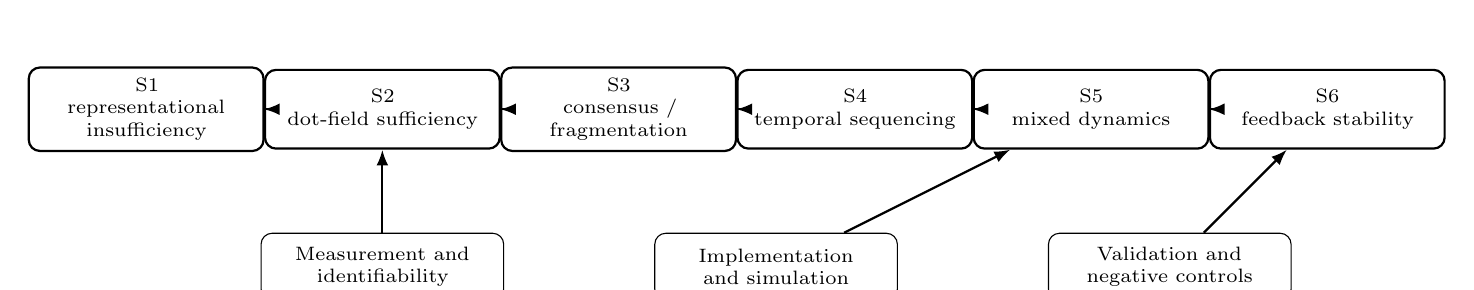
\begin{tikzpicture}[
  x=1cm,y=1cm,
  spine/.style={draw, rounded corners, thick, align=center, text width=2.7cm, minimum height=1.0cm, font=\scriptsize, inner sep=4pt},
  support/.style={draw, rounded corners, align=center, text width=2.8cm, minimum height=0.85cm, font=\scriptsize, inner sep=4pt},
  arr/.style={-{Latex[length=2mm]}, thick}
]
\node[spine] (s1) at (0,0) {S1\\representational insufficiency};
\node[spine] (s2) at (3.0,0) {S2\\dot-field sufficiency};
\node[spine] (s3) at (6.0,0) {S3\\consensus / fragmentation};
\node[spine] (s4) at (9.0,0) {S4\\temporal sequencing};
\node[spine] (s5) at (12.0,0) {S5\\mixed dynamics};
\node[spine] (s6) at (15.0,0) {S6\\feedback stability};
\foreach \a/\b in {s1/s2,s2/s3,s3/s4,s4/s5,s5/s6}{\draw[arr] (\a) -- (\b);}
\node[support] (meas) at (3.0,-2.0) {Measurement and identifiability};
\node[support] (impl) at (8.0,-2.0) {Implementation and simulation};
\node[support] (val) at (13.0,-2.0) {Validation and negative controls};
\draw[arr] (meas) -- (s2); \draw[arr] (impl) -- (s5); \draw[arr] (val) -- (s6);
\end{tikzpicture}%
}
\caption{Primary theorem spine. The main formal path begins with representational insufficiency and state sufficiency, then develops convergence, order sensitivity, mixed-mechanism composition, and recursive feedback stability. Measurement, implementation, and validation results support rather than replace the spine.}
\label{fig:theorem-spine}
\end{figure}


\subsection{Proof-priority convention}\label{proof-priority-convention}

The paper uses theorem environments according to a priority convention. Core theorems state representation, sufficiency, convergence, order-dependence, composition, or stability results. Propositions state mechanism-specific implications, threshold conditions, bounds, or recoverability statements. Corollaries record direct consequences of a theorem or proposition. Lemmas are reserved for intermediate facts needed in proofs. This convention makes the proof architecture auditable: the main claims are concentrated in the theorem spine, while supporting results are explicitly subordinate. To avoid proof repetition, direct corollaries are stated without separate proof when they follow immediately by specialization, projection, or monotonicity from the preceding theorem or proposition. Proofs are retained for core theorems, technical lemmas, and mechanism claims whose assumptions require verification.

\subsection{Assumption register}\label{assumption-register}

The following assumption register collects the recurring assumptions used by the theorem family. Later theorem statements may specialize these assumptions, but they should not silently require stronger conditions.

{\small
\begin{longtable}{L{0.10\linewidth}L{0.22\linewidth}L{0.34\linewidth}L{0.12\linewidth}}
\caption{Assumption register for the theorem family.}\label{tab:assumption-register}\\
\toprule
\textbf{Code} & \textbf{Name} & \textbf{Content} & \textbf{Used by}\\
\midrule
\endfirsthead
\toprule
\textbf{Code} & \textbf{Name} & \textbf{Content} & \textbf{Used by}\\
\midrule
\endhead
A1 & Memory sensitivity & Retrieved dots can change an agent's action distribution after conditioning on ordinary state variables. & T1, validation\\
A2 & Dot-state completeness & The chosen dot state encodes all transition-relevant historical information for the modeled process. & T2\\
A3 & Fixed vocabulary phase & The dot vocabulary is fixed, or mapped to a fixed reference vocabulary, during the analyzed consensus interval. & T3, T4\\
A4 & Stochastic influence & The influence matrix is row-stochastic; connectedness, primitivity, or block structure is stated as needed. & T3, T4\\
A5 & Non-commutative assimilation & Some dot assimilation or exchange operators fail to commute. & T5\\
A6 & Institutional persistence & Institutional dots have stronger persistence, reach, credibility, or retrievability than private dots under specified parameters. & T6\\
A7 & Dot-responsive topology & Social edges update as functions of retrieved evaluative dot pressure. & T7\\
A8 & Effective correction & Counter-dots have accessible, credible, and semantically fitted correction pressure. & T8\\
A9 & Bounded semantic representation & Dot meanings can be represented in a semantic space with a usable distance or equivalence threshold. & T9\\
A10 & Observation model & The data-generating and observation processes specify which dots, accesses, relations, actions, and edges are observed or latent. & T10, measurement\\
A11 & Typed implementation & Implementation routines preserve identifiers, types, access rules, relation validity, weight bounds, and lineage constraints. & Algorithmic results\\
A12 & No leakage validation & Prediction records are created before the outcome, and train-test splits prevent future information from entering training features. & Validation results\\
A13 & Mixed-mechanism validity & Active mechanism operators are typed, measurable, state-validity preserving, and explicitly ordered or justified when order matters. & Integrated dynamics\\
A14 & Recursive topology feedback & Edge-sensitive access, access-sensitive retrieval, retrieval-sensitive pressure, and pressure-sensitive edge updates are specified with Lipschitz, differentiability, threshold, or empirical linearization conditions. & Stability layer\\
\bottomrule
\end{longtable}
}

\subsection{Theorem register}\label{theorem-register}

Table~\ref{tab:theorem-register} gives the consolidated register for the theorem family. The observability column uses the measurement ladder introduced later in the paper: O0 is action-only data; O1 adds social edges; O2 adds communications or artifacts; O3 adds provenance and access; O4 adds logged retrieval, attention, or institutional access; O5 adds randomized exposure or instrumented memory. A theorem can be valid at the formal level even when a dataset falls below the listed grade; in that case, the empirical claim should be weakened.

{\scriptsize
\begin{longtable}{@{}L{0.15\linewidth}L{0.12\linewidth}L{0.17\linewidth}L{0.32\linewidth}L{0.08\linewidth}@{}}
\caption{Theorem register by state scope and empirical observability.}\label{tab:theorem-register}\\
\toprule
\textbf{Result} & \textbf{Class} & \textbf{State scope} & \textbf{Main assumption burden} & \textbf{Test grade}\\
\midrule
\endfirsthead
\toprule
\textbf{Result} & \textbf{Class} & \textbf{State scope} & \textbf{Main assumption burden} & \textbf{Test grade}\\
\midrule
\endhead
Rep. insufficiency & Core & $Z_t$ versus $\Omega_t^{core}$ & A1 and existence of omitted accessible dots that change action. & O2--O4\\
Dot-sufficient comp. & Core & Projection of $\Omega_t^{core}$ into a reduced statistic & The reduced statistic preserves all transition-relevant dot effects. & O3--O5\\
Markov restoration & Core & $\Omega_t^{aug}$, or $\Omega_t^{core}$ if sufficient & A2; no omitted history changes the next transition. & O3--O5\\
Mixed dynamics & Mechanism & $\Omega_t^{aug}$ and active operator set & A13; operators are typed, measurable, validity-preserving, and order-declared. & O2--O5 or simulated\\
Recursive feedback & Mechanism & $E_t,B_t,\mathcal V_t,\boldsymbol{\zeta}_t$ & A14; feedback maps are Lipschitz, differentiable, thresholded, or empirically linearized. & O3--O5 or simulated\\
Dot consensus & Mechanism & $\mathbf M_t$ over fixed $D$ & A3--A4 with connected or primitive influence. & O2--O4\\
Fragmented memory & Mechanism & $\mathbf M_t$ and block social influence & A3--A4 with disconnected or weakly bridged components. & O2--O4\\
Temporal sequencing & Mechanism & Ordered dot sequences and assimilation operators & A5; sequence or exchange order is observed or controlled. & O3--O5\\
Institutional stabil. & Mechanism & $\Omega_t^{aug}$ with $I_t$ and $Q_t$ & A6 with measurable persistence, reach, or authority. & O2--O4\\
Dot-induced topology & Mechanism & $\Omega_t^{aug}$ with evaluative dots and $E_t$ & A7; edges respond to retrieved evaluative pressure. & O2--O4\\
Counter-dot correction & Mechanism & $\Omega_t^{aug}$ with $C_t$ and $Q_t$ & A8; counter-dot reach, fit, and credibility are measurable or simulated. & O3--O5\\
Mutation and compression & Mechanism & $\Omega_t^{aug}$ with $L_t$ and semantic states & A9; lineage or semantic equivalence is defined. & O3--O5\\
Identifiability & Measure. & observation model & A10; observation channels and parameter restrictions are specified. & O0--O5\\
Extraction-error & Measure. & estimated dot field & Extraction error is bounded and the policy is Lipschitz in extracted features. & O2--O5\\
Alg. valid. & Impl. & impl. state & A11; typed routines preserve invariants. & Sim.\\
Sim. faith. & Impl. & projection & Simulator routines implement formal operations. & Sim.\\
Prediction-lift theorem & Validation & $Z_t$ versus $\Omega_t^{aug}$ features & Proper scoring, no leakage, and transition-relevant dot information. & O1--O5\\
Trainable held-out lift & Validation & Fitted feature classes from $Z_t$ and $\Omega_t^{aug}$ & A12 and risk-consistent learning under temporal separation. & O1--O5\\
Negative-control degradation & Validation & Corrupted dot features & Controls destroy alignment while preserving marginal structure. & O2--O5\\
\bottomrule
\end{longtable}
}

\subsection{Measurement-theorem compatibility principle}\label{measurement-theorem-compatibility-principle}

A theorem should not be converted into an empirical claim unless the observed data support the objects on which the theorem depends. Formally, let $g(\Omega_t^{aug})$ be the theorem-relevant dot quantity and let $Y_{0:T}$ be the available observation record. An empirical use of the theorem is measurement-admissible only when either:
\[
 g(\Omega_t^{aug}) \text{ is observed or consistently estimable from } Y_{0:T},
\]
or the study explicitly treats it as latent and reports the resulting ambiguity or sensitivity set. Otherwise, the result can still guide conceptual interpretation or simulation, but it should not be presented as directly supported by the data.

This principle is especially important for access, retrieval, credibility, and counter-dot reach. A communication log may show that a dot existed; it does not automatically show that each agent accessed it, attended to it, retrieved it, trusted it, or acted on it.

\subsection{Consolidated proof obligations}\label{consolidated-proof-obligations}

The proof obligations for a dot-field result are now the following.

\begin{enumerate}[leftmargin=*]
\item \textbf{State obligation:} identify whether the theorem uses $Z_t$, $\Omega_t^{core}$, $\Omega_t^{aug}$, or $\mathsf S_t$.
\item \textbf{Projection obligation:} state what is lost when the theorem projects from a richer state to a poorer state.
\item \textbf{Mechanism obligation:} specify which dot mechanism is active: retrieval, transmission, mutation, compression, correction, institutionalization, or topology feedback.
\item \textbf{Assumption obligation:} cite the required assumptions from the register or define new ones locally.
\item \textbf{Measurement obligation:} state the minimum observability grade needed to test the result outside simulation.
\item \textbf{Failure obligation:} state what would make the theorem inapplicable or the empirical claim fail.
\end{enumerate}

The remaining theorem sections should be read against these obligations. This consolidation is deliberately conservative: it makes the theory less sweeping, but more defensible.

\section{Main Theoretical Results}\label{theoretical-results}

This section develops the formal core of the article. The results are conditional: each holds under explicit assumptions and each targets a specific representational, dynamic, measurement, implementation, or validation question. The section should be read with the state-scope convention, primary theorem spine, and proof-priority convention in Section~\ref{theorem-consolidation-state-assumptions-measurement}. The first two subsections supply the core representation results: insufficiency of the reduced agent-edge projection and conditional restoration of state sufficiency by the dot-augmented state. The subsequent subsections provide mechanism and measurement results that extend the spine to consensus, fragmentation, sequencing, institutionalization, topology feedback, correction, semantic drift, compression, and identifiability. Direct corollaries are recorded as consequences rather than re-proved; this keeps the proof path focused on the theorem spine while preserving the supporting implications.

\paragraph{Proof-spine reading guide.} The six spine results should be read as the formal backbone of the theory. S1 establishes that reduced agent-edge states can omit transition-relevant traces. S2 gives the corresponding state-lift condition. S3 characterizes convergence and fragmentation under dot exchange. S4 shows why order matters when assimilation operators do not commute. S5 composes the mechanisms into a single transition system. S6 analyzes stability of the recursive topology-memory loop. The additional propositions and corollaries refine these mechanisms without changing the central proof path.

\subsection{Representational insufficiency}\label{representational-insufficiency}

\paragraph{Consolidated scope.} This is a core representation theorem. It compares the reduced state $Z_t$ against a core dot field $\Omega_t^{core}$ and requires memory sensitivity (A1). Empirical tests require at least observed actions and enough trace evidence to distinguish accessible dot conditions; action-only data can show behavioral divergence but cannot identify dot composition.

This result is the formal anchor of Dot-Trace Theory. It states that a
social graph over agents can be an insufficient state description when
agents act on retrieved traces. The point is not that every dot must be
represented explicitly in every practical model. The point is that, for
the class of memory-sensitive social systems, any sufficient
representation must contain either the relevant dots themselves or a
sufficient statistic of them.

\begin{definition}[Core dot state]
For the purpose of the representation theorem, let the core dot state be
$$
\Omega_t^{core}=(A,E_t,X_t,\bar S_t,D_t,R_t^D,B_t),
$$
where $A$ is the agent set, $E_t$ is the social edge structure, $X_t$ is the environmental state, $\bar S_t$ is the collection of non-dot agent state variables, $D_t$ is the dot set, $R_t^D$ is the dot-dot relation structure, and $B_t$ is the agent-dot access structure. When this subsection uses the shorter symbol $\Omega_t$, it refers to this core dot state unless an augmented state is explicitly named.
\end{definition}

\begin{definition}[Agent-edge projection]
The agent-edge projection of the core dot state is
$$
Z_t=\rho_Z(\Omega_t^{core})=(A,E_t,X_t,\bar S_t).
$$
It deliberately omits $D_t$, $R_t^D$, and $B_t$. Thus $Z_t$ represents the ordinary agent-edge description of the social system, not the dot field.
\end{definition}

\begin{definition}[Transition sufficiency]
A representation $Z_t=\rho_Z(\Omega_t^{core})$ is transition-sufficient for an outcome $Y_{t+1}$ on a class of systems if, whenever two core dot states $\Omega_t^{core}$ and $\Omega_t^{core\prime}$ have the same representation,
$$
\rho_Z(\Omega_t^{core})=\rho_Z(\Omega_t^{core\prime}),
$$
they also induce the same conditional distribution over the next outcome:
$$
P(Y_{t+1}\mid \Omega_t^{core})=P(Y_{t+1}\mid \Omega_t^{core\prime}).
$$
If this condition fails, then $Z_t$ is not sufficient for predicting $Y_{t+1}$.
\end{definition}

\begin{assumption}[Non-degenerate memory sensitivity]
There exists at least one agent $a_i$, one decision context $q$, one action $u$, and two accessible dot sets $M$ and $M'$ such that all non-dot state variables are identical but the action distribution differs:
$$
P_i(u\mid o_i,\bar s_i,q,\mathcal V_i(q,M))
\neq
P_i(u\mid o_i,\bar s_i,q,\mathcal V_i(q,M')).
$$
This assumption rules out the trivial case in which memory exists but has no effect on action.
\end{assumption}

\begin{lemma}[Agent-edge observational equivalence]
There exist core dot states $\Omega_t^{core}$ and $\Omega_t^{core\prime}$ such that
$$
\rho_Z(\Omega_t^{core})=\rho_Z(\Omega_t^{core\prime})
$$
but
$$
(D_t,R_t^D,B_t)\neq (D_t^{\prime},R_t^{D\prime},B_t^{\prime}).
$$
\end{lemma}

\begin{proof}
The projection $\rho_Z$ deletes the dot set, dot-dot relations, and agent-dot access relations. Therefore, any two states that agree on $A$, $E_t$, $X_t$, and $\bar S_t$, but differ only in $D_t$, $R_t^D$, or $B_t$, have the same projected representation. Such states exist whenever at least one accessible dot can differ while the social graph and non-dot variables are held fixed. Hence the claim follows by construction.
\end{proof}

\begin{theorem}[Representational insufficiency]\label{thm:representational-insufficiency}
For the class of non-degenerate memory-sensitive social multi-agent systems, the agent-edge projection
$$
Z_t=(A,E_t,X_t,\bar S_t)
$$
is not transition-sufficient in general. In particular, there exist two core dot states with identical agent-edge projections but different future action distributions.
\end{theorem}

\begin{proof}
We prove the result by construction.

Let the agent set contain at least two agents, $a_i$ and $a_j$. At time $t$, agent $a_i$ must choose whether to cooperate with $a_j$. Let the action set be
$$
\mathcal{U}_i=\{C,D\},
$$
where $C$ denotes cooperation and $D$ denotes defection.

Construct two core dot states, $\Omega_t^{core,+}$ and $\Omega_t^{core,-}$, with the same agent-edge projection:
$$
\rho_Z(\Omega_t^{core,+})=\rho_Z(\Omega_t^{core,-}).
$$
Thus both states have the same agents, same social graph, same environmental state, same non-dot agent states, and same current observation for $a_i$. In particular,
$$
w_{ij}^{trust,+}(t)=w_{ij}^{trust,-}(t),
$$
and
$$
o_i^+(t)=o_i^-(t), \qquad \bar s_i^+(t)=\bar s_i^-(t).
$$

The two states differ only in the dot-access layer. In $\Omega_t^{core,+}$, agent $a_i$ can access a positive dot about $a_j$:
$$
d^+ = \text{``agent } a_j \text{ helped agent } a_i \text{ before.''}
$$
In $\Omega_t^{core,-}$, agent $a_i$ can access a negative dot about $a_j$:
$$
d^- = \text{``agent } a_j \text{ betrayed agent } a_i \text{ before.''}
$$
Equivalently,
$$
(a_i,d^+)\in B_t^+, \qquad (a_i,d^-)\in B_t^-,
$$
with the projected social state unchanged.

Let the decision context be $q=$ ``decide whether to cooperate with $a_j$.'' Suppose the retrieval function returns the relevant accessible dot in each state:
$$
\mathcal V_i^+(q,t)=\{d^+\}, \qquad \mathcal V_i^-(q,t)=\{d^-\}.
$$
Assign dot valences
$$
v_i(d^+)=1, \qquad v_i(d^-)=-1.
$$
Let the policy of $a_i$ be memory-sensitive, with cooperation probability
$$
P_i(C\mid o_i,\bar s_i,q,\mathcal V_i)=\sigma\left(\beta_0+\beta_1\sum_{d\in \mathcal V_i}v_i(d)\right),
$$
where $\sigma(x)=1/(1+e^{-x})$ is strictly increasing and $\beta_1>0$.

Then in the positive-dot state,
$$
P_i(C\mid \Omega_t^{core,+})=\sigma(\beta_0+\beta_1),
$$
while in the negative-dot state,
$$
P_i(C\mid \Omega_t^{core,-})=\sigma(\beta_0-\beta_1).
$$
Since $\beta_1>0$ and $\sigma$ is strictly increasing,
$$
P_i(C\mid \Omega_t^{core,+}) > P_i(C\mid \Omega_t^{core,-}).
$$

However, the agent-edge projection is identical in the two states:
$$
Z_t^+=\rho_Z(\Omega_t^{core,+})=\rho_Z(\Omega_t^{core,-})=Z_t^-.
$$
Any model that conditions only on $Z_t$ must assign the same predicted probability to cooperation in both states:
$$
Q(C\mid Z_t^+)=Q(C\mid Z_t^-).
$$
It therefore cannot equal both true probabilities when those probabilities differ. Hence the agent-edge projection is not transition-sufficient for the next action outcome. Since agent action contributes to subsequent dot creation, access updates, and social edge updates, the insufficiency also propagates to the next system transition. Therefore, agent-edge representations are not sufficient in general for non-degenerate memory-sensitive social multi-agent systems.
\end{proof}

\begin{corollary}[Dot-sufficient compression]
An agent-edge model can be sufficient for a memory-sensitive system only if its state variables encode all dot information that is relevant to future transitions. In that case, the representation is no longer purely dot-free; it contains a dot-sufficient statistic.
\end{corollary}

\begin{proof}
Assume an agent-edge representation $Z_t$ is sufficient even though the system is memory-sensitive. By transition sufficiency, any two full states with the same $Z_t$ must induce the same future transition distribution. Therefore, whenever two dot fields would change future action or transition probabilities, they cannot share the same value of $Z_t$. It follows that $Z_t$ must distinguish all transition-relevant dot differences, either by storing the dots explicitly or by storing a statistic that preserves their causal effect. Such a representation is dot-sufficient, even if it is not dot-explicit. Therefore, pure omission of transition-relevant dot structure is impossible under sufficiency.
\end{proof}

\begin{remark}[Interpretation]
The theorem is an insufficiency result, not a claim that every practical model must store every trace verbatim. Compression is allowed. Edge weights, reputational scores, embeddings, or agent state variables may summarize dot histories. But if they summarize the histories well enough to preserve future action distributions, then they are functioning as dot-sufficient representations. Dot-Trace Theory makes this hidden dependence explicit.
\end{remark}

\subsection{Dot-field Markov restoration}\label{dot-field-markov-restoration}

\paragraph{Consolidated scope.} This is a core state-lifting theorem. In the canonical hierarchy the relevant state is $\Omega_t^{aug}$ unless memory weights, effective strengths, lineages, institutional stores, and correction states are deterministic functions of $\Omega_t^{core}$. The theorem requires complete dot-state encoding (A2) and should be interpreted as a conditional sufficiency result, not as a universal claim that any chosen dot field is Markov-sufficient.

The first theorem established a negative claim: an agent-edge projection
can be insufficient when agents are memory-sensitive. The second theorem
states the corresponding positive claim. If the transition-relevant past
is encoded in the current dot field, then the dot-augmented state
restores the Markov property. In this sense, dots do not eliminate path
dependence; they represent path dependence as present structure.

\begin{definition}[Pre-dot history]
Let $\mathcal{H}_t$ denote the complete observable and latent history of
an underlying social process up to time $t$. It may include prior
environmental states, social edges, observations, actions,
communications, events, records, retrievals, and institutional updates:
$$
\mathcal{H}_t=(X_0,E_0,\bar S_0,O_0,U_0,Ev_0,\ldots,X_t,E_t,\bar S_t,O_t).
$$
The exact content of $\mathcal{H}_t$ may vary by model. Its role is to
represent the full past that could, in principle, influence the future.
\end{definition}

\begin{definition}[Dot encoding map]
A dot encoding map is a history compression
$$
\Gamma_t:\mathcal{H}_t\rightarrow (D_t,R_t^D,B_t,\mathbf M_t,Q_t,L_t,I_t,C_t),
$$
where $D_t$ is the dot set, $R_t^D$ is the dot-dot relation structure, $B_t$ is the agent-dot access structure, $\mathbf M_t$ stores dot weights, $Q_t$ stores effective strengths, $L_t$ stores lineage and provenance, $I_t$ stores institutional encodings, and $C_t$ stores correction state. Let $\Xi_t$ denote the induced full state encoding. The dot-augmented state is
$$
\Omega_t^{aug}=\Xi_t(\mathcal{H}_t)=(A,E_t,X_t,\bar S_t,D_t,R_t^D,B_t,\mathbf M_t,Q_t,L_t,I_t,C_t),
$$
with the core dot field recovered by projection. In this subsection, the shorter symbol $\Omega_t$ denotes $\Omega_t^{aug}$ unless a projection is explicitly named.
\end{definition}

\begin{definition}[Transition-relevant equivalence]
Two histories $h_t$ and $h'_t$ are dot-equivalent when they induce the
same augmented dot-field state:
$$
\Xi_t(h_t)=\Xi_t(h'_t).
$$
A dot encoding is transition-sufficient when, for every measurable set
$C$ of possible next dot-augmented states,
$$
P(\Omega_{t+1}\in C\mid \mathcal{H}_t=h_t)
=
P(\Omega_{t+1}\in C\mid \mathcal{H}_t=h'_t)
$$
whenever $\Xi_t(h_t)=\Xi_t(h'_t)$.
\end{definition}

\begin{assumption}[Complete dot encoding]
All historically relevant information affecting the next transition is
encoded in the current dot-augmented state $\Omega_t^{aug}$. Equivalently,
after conditioning on $\Omega_t$, no omitted part of $\mathcal{H}_t$
changes the conditional distribution of the next observation, retrieval,
action, event, dot-update, access-update, topology-update, or
environment-update step.

Formally, the one-step dynamics can be expressed by kernels of the form
$$
\mathsf{K}_O(O_t\mid \Omega_t),
$$
$$
\mathsf{K}_{Ret}(\mathcal V_t\mid O_t,\Omega_t),
$$
$$
\mathsf{K}_{U}(U_t\mid \mathcal V_t,O_t,\Omega_t),
$$
$$
\mathsf{K}_{Ev}(Ev_t\mid U_t,\Omega_t),
$$
$$
\mathsf{K}_{D}(D_{t+1},R_{t+1}^D\mid Ev_t,U_t,\Omega_t),
$$
$$
\mathsf{K}_{B}(B_{t+1}\mid Ev_t,U_t,D_{t+1},R_{t+1}^D,\Omega_t),
$$
$$
\mathsf{K}_{E}(E_{t+1}\mid Ev_t,U_t,D_{t+1},R_{t+1}^D,B_{t+1},\Omega_t),
$$
and
$$
\mathsf{K}_{X}(X_{t+1},\bar S_{t+1}\mid Ev_t,U_t,E_{t+1},D_{t+1},R_{t+1}^D,B_{t+1},\Omega_t).
$$
Here $\mathcal V_t$ denotes the collection of retrieved-dot sets or retrieval outputs. The symbol $Q_t$ is reserved for effective retrievable strengths in the augmented state. The assumption does not require deterministic dynamics; it only requires that the stochastic kernels depend on the past through $\Omega_t$.
\end{assumption}

\begin{lemma}[Screening-off lemma]
Under complete dot encoding, if two histories $h_t$ and $h'_t$ satisfy
$$
\Xi_t(h_t)=\Xi_t(h'_t)=\Omega_t,
$$
then they induce the same conditional distribution over
$\Omega_{t+1}$.
\end{lemma}

\begin{proof}
Fix histories $h_t$ and $h'_t$ that induce the same augmented state $\Omega_t$. Complete dot encoding states that every one-step kernel for observation, retrieval, action, event generation, dot update, access update, topology update, and environmental update depends on the past only through $\Omega_t$ and variables generated during the current step. Hence both histories induce the same distribution over the first intermediate variable, the same conditional distribution over the second given the first, and so on through the composed transition. Therefore, for every measurable next-state event $C$,
$$
P(\Omega_{t+1}\in C\mid \mathcal{H}_t=h_t)
=
P(\Omega_{t+1}\in C\mid \mathcal{H}_t=h'_t),
$$
so the current dot-augmented state screens off earlier history from the next transition.
\end{proof}

\begin{theorem}[Dot-field Markov restoration]\label{thm:dot-field-markov-restoration}
If the dot encoding is complete in the sense above, then the
augmented dot-field state
$$
\Omega_t^{aug}=(A,E_t,X_t,\bar S_t,D_t,R_t^D,B_t,\mathbf M_t,Q_t,L_t,I_t,C_t)
$$
is Markovian. That is, there exists a transition kernel
$\mathsf{K}_\Omega$ such that, for every measurable set $C$ of possible
next dot-augmented states,
$$
P(\Omega_{t+1}\in C\mid \mathcal{H}_t)
=
\mathsf{K}_\Omega(C\mid \Omega_t).
$$
Equivalently,
$$
P(\Omega_{t+1}\mid \Omega_t,\Omega_{t-1},\ldots,\Omega_0)
=
P(\Omega_{t+1}\mid \Omega_t).
$$
\end{theorem}

\begin{proof}
By the screening-off lemma, any two histories that induce the same
current dot-augmented state induce the same conditional distribution
over the next dot-augmented state. Hence the conditional distribution of
$\Omega_{t+1}$ is a function only of $\Omega_t$, not of the particular
history by which $\Omega_t$ was reached.

Define $\mathsf{K}_\Omega(C\mid \omega)$ as the common value of
$$
P(\Omega_{t+1}\in C\mid \mathcal{H}_t=h_t)
$$
for any history $h_t$ such that $\Xi_t(h_t)=\omega$. This definition is
well-defined because the screening-off lemma guarantees that all such
histories produce the same conditional distribution. Therefore,
$$
P(\Omega_{t+1}\in C\mid \mathcal{H}_t)=\mathsf{K}_\Omega(C\mid \Omega_t).
$$
Since $(\Omega_0,\ldots,\Omega_t)$ is itself a sub-history of
$\mathcal{H}_t$, conditioning on earlier dot-augmented states cannot add
transition-relevant information beyond $\Omega_t$. Thus,
$$
P(\Omega_{t+1}\mid \Omega_t,\Omega_{t-1},\ldots,\Omega_0)
=
P(\Omega_{t+1}\mid \Omega_t),
$$
which is the Markov property for the dot-augmented process.
\end{proof}

\begin{corollary}[Path dependence represented as state]
Dot-field Markov restoration does not imply that the social system is
history-free. It implies that history has been encoded into the present
state. Earlier events can still affect future behavior through the dots,
relations, access patterns, salience values, credibility values, and
edge weights that they leave behind.
\end{corollary}


\begin{corollary}[Projection can destroy Markovianity]
Let
$$
Z_t=\rho_Z(\Omega_t^{aug})=(A,E_t,X_t,\bar S_t)
$$
be the agent-edge projection. Even if $\Omega_t$ is Markovian, $Z_t$
need not be Markovian. In particular, if two dot states share the same
projection but induce different future transitions, then
$$
P(Z_{t+1}\mid Z_t,Z_{t-1},\ldots,Z_0)
\neq
P(Z_{t+1}\mid Z_t)
$$
in general.
\end{corollary}


\begin{corollary}[Dot compression and non-uniqueness]
Markov restoration does not require storing the full literal history.
Any representation that preserves all transition-relevant historical
information can serve as a dot encoding. Therefore, dot fields are not
unique: different encodings may be equivalent if they induce the same
transition kernel $\mathsf{K}_\Omega$.
\end{corollary}


\begin{proposition}[Failure condition]
If there exists an omitted historical variable $H_t^{omit}$ such that
$$
P(\Omega_{t+1}^{aug}\mid \Omega_t^{aug},H_t^{omit})\neq P(\Omega_{t+1}^{aug}\mid \Omega_t^{aug}),
$$
then the proposed dot field is not complete and Markov restoration
fails for that state specification.
\end{proposition}

\begin{proof}
The inequality states directly that, after conditioning on $\Omega_t$,
an omitted part of the past still changes the next-state distribution.
Therefore, $\Omega_t$ does not screen off history and cannot satisfy the
Markov property. The remedy is to extend the dot field or another state
component until the omitted variable is encoded or shown to be
transition-irrelevant.
\end{proof}

\begin{remark}[Relation to the first theorem]
The first theorem shows why agent-edge projections are insufficient in
memory-sensitive systems. The second theorem shows how dot augmentation
can repair that insufficiency under an explicit completeness condition.
Together, the results justify the central state object of the theory:
the dot field is not merely a descriptive convenience, but a candidate
state-lift that turns remembered history into processable present
structure.
\end{remark}

\subsection{Dot consensus}\label{dot-consensus}

\paragraph{Consolidated scope.} This is a mechanism theorem over the dot-weight matrix $\mathbf M_t$ during a fixed-vocabulary phase. It requires a row-stochastic influence matrix and connectedness or primitivity assumptions (A3--A4). Empirical testing requires comparable dot coordinates across agents; without a shared vocabulary or alignment map, consensus is not well-defined.

The first two theorems justify why dots are needed as part of the state
representation. The next theorem studies one simple dynamic consequence
of dot exchange: when agents repeatedly update their dot weights through
a connected social influence network, their accessible dot weights can
converge to a shared collective memory vector. This result should be
read as a deliberately restricted baseline. It assumes a fixed dot
vocabulary, no mutation, no deletion, no new dot creation, and linear
averaging. Later models can relax these assumptions.

\begin{definition}[Dot-weight matrix]
Fix a reference dot vocabulary
$$
D^*=\{d_1,\ldots,d_K\}.
$$
Agent $a_i$'s weight vector over this vocabulary at time $t$ is
$$
m_i(t)=(m_{i1}(t),\ldots,m_{iK}(t))\in \mathbb{R}^K,
$$
where $m_{ik}(t)$ may represent the salience, credibility, acceptance,
or practical decision weight assigned by agent $a_i$ to dot $d_k$. Stack
these row vectors into the matrix
$$
M(t)=
\begin{bmatrix}
 m_1(t) \\
 \vdots \\
 m_n(t)
\end{bmatrix}
\in \mathbb{R}^{n\times K}.
$$
The $k$th column of $M(t)$ records the distribution of one dot's weight
across all agents.
\end{definition}

\begin{definition}[Lazy dot-exchange update]
Let $W\in\mathbb{R}^{n\times n}$ be a row-stochastic influence matrix,
so that $W_{ij}\geq 0$ and $\sum_j W_{ij}=1$ for every agent $i$. The
linear dot-exchange update is
$$
M(t+1)=P M(t),
$$
where
$$
P=\lambda I+(1-\lambda)W,\qquad 0<\lambda<1.
$$
The parameter $\lambda$ represents self-retention: an agent keeps part
of its prior dot-weight vector and averages the remainder through social
influence.
\end{definition}

\begin{assumption}[Consensus phase]
During the consensus phase, the following conditions hold:
\begin{enumerate}[label=(C\arabic*)]
\item the reference dot vocabulary $D^*$ is fixed;
\item no dots are created, deleted, or semantically mutated;
\item dot weights are updated by the lazy dot-exchange rule;
\item $W$ is fixed, nonnegative, row-stochastic, and irreducible;
\item $0<\lambda<1$.
\end{enumerate}
\end{assumption}

Irreducibility means that the influence graph associated with $W$ is
strongly connected: each agent can influence each other agent through
some finite path, although not necessarily in one step.

\begin{lemma}[Primitivity of the lazy influence matrix]
Under the consensus phase assumptions, $P=\lambda I+(1-\lambda)W$ is
row-stochastic and primitive.
\end{lemma}

\begin{proof}
Since $I$ and $W$ are row-stochastic and $P$ is their convex
combination, $P$ is row-stochastic:
$$
P\mathbf{1}=\lambda I\mathbf{1}+(1-\lambda)W\mathbf{1}
=\lambda\mathbf{1}+(1-\lambda)\mathbf{1}=\mathbf{1}.
$$
All entries of $P$ are nonnegative because $I$ and $W$ are nonnegative.
Moreover, whenever $W_{ij}>0$ with $i\neq j$, we also have
$P_{ij}=(1-\lambda)W_{ij}>0$. Thus $P$ contains the same off-diagonal
communication paths as $W$, so irreducibility of $W$ implies
irreducibility of $P$.

Finally, for every $i$,
$$
P_{ii}=\lambda+(1-\lambda)W_{ii}\geq \lambda>0.
$$
Thus every state has a self-loop. A finite irreducible stochastic matrix
with a positive diagonal is aperiodic. A finite stochastic matrix that is
irreducible and aperiodic is primitive. Therefore $P$ is primitive.
\end{proof}

\begin{theorem}[Dot consensus]\label{thm:dot-consensus}
Under the consensus phase assumptions, there exists a unique stationary
influence vector $\pi\in\mathbb{R}^n$ satisfying
$$
\pi_j\geq 0,\qquad \sum_j \pi_j=1,\qquad \pi^\top P=\pi^\top,
$$
and the dot-weight matrix converges to
$$
\lim_{t\to\infty}M(t)=\mathbf{1}\pi^\top M(0).
$$
Equivalently, for every agent $i$ and every dot $d_k$,
$$
\lim_{t\to\infty}m_{ik}(t)=\sum_{j=1}^n \pi_j m_{jk}(0).
$$
Thus all agents converge to the same dot-weight vector, equal to a
stationary-influence-weighted aggregate of the initial dot weights.
\end{theorem}

\begin{proof}
By the lemma, $P$ is primitive and row-stochastic. The
Perron--Frobenius theorem for primitive stochastic matrices implies that
$P$ has a unique stationary distribution $\pi$ with positive entries and
that
$$
\lim_{t\to\infty}P^t=\mathbf{1}\pi^\top.
$$
Iterating the update rule gives
$$
M(t)=P^tM(0).
$$
Taking limits,
$$
\lim_{t\to\infty}M(t)
=\left(\lim_{t\to\infty}P^t\right)M(0)
=\mathbf{1}\pi^\top M(0).
$$
The matrix $\mathbf{1}\pi^\top M(0)$ has identical rows, so every agent
converges to the same dot-weight vector. Reading the $k$th coordinate of
that row gives
$$
\lim_{t\to\infty}m_{ik}(t)=\sum_{j=1}^n \pi_jm_{jk}(0),
$$
for every agent $i$ and every dot $d_k$.
\end{proof}

\begin{corollary}[Collective dot memory as a limiting vector]
Under the conditions of Theorem~\ref{thm:dot-consensus}, the limiting
collective memory of the group can be represented as
$$
\bar m=\pi^\top M(0)\in\mathbb{R}^{1\times K}.
$$
The group does not merely converge to a shared scalar opinion; it
converges to a shared vector of dot weights.
\end{corollary}


\begin{corollary}[Unequal influence and dot-mediated social capital]
The contribution of agent $a_j$'s initial weight for dot $d_k$ to the
limiting collective weight of that dot is $\pi_j$:
$$
\frac{\partial \bar m_k}{\partial m_{jk}(0)}=\pi_j.
$$
Therefore, agents with larger stationary influence weights have greater
capacity to shape the collective dot field during linear consensus.
\end{corollary}


This corollary clarifies the connection to social capital. In this
restricted model, structural position is encoded in $\pi$, while the
valuable or harmful trace content is encoded in $M(0)$. Social capital
is not identical to either one. It emerges from the coupling between
access to valuable dots, credibility in transmitting them, and influence
within the social graph.

\begin{corollary}[Centroid and barycenter interpretation]
The consensus vector $\bar m=\pi^\top M(0)$ is a barycenter in dot-weight
space. If $\pi_j=1/n$ for all agents, then
$$
\bar m=\frac{1}{n}\sum_{j=1}^n m_j(0),
$$
which is the ordinary centroid of the agents' initial dot-weight
vectors. If $\pi$ is non-uniform, then $\bar m$ is a weighted centroid.
\end{corollary}


The centroid statement should be read carefully. A dot is not, by
definition, the centroid of the social network. A dot is a trace object.
The consensus vector is a centroid-like object in dot-weight space, not
inside the ordinary agent-agent graph. Separately, in the lifted
heterogeneous graph
$$
H_t=(A\cup D_t,E_t\cup R_t^D\cup B_t),
$$
a particular dot may become a central memory hub if many agents access
it or if many other dots link to it. That is a derived centrality
property, not the definition of a dot.

\begin{proposition}[Spectral rate of dot consensus]
Suppose, in addition, that $P$ is diagonalizable over $\mathbb{C}$. Let
$$
\rho_* = \max\{ |\mu| : \mu \text{ is an eigenvalue of }P,\ \mu\neq 1\}.
$$
Then $\rho_*<1$, and there exists a constant $C>0$ such that
$$
\|M(t)-\mathbf{1}\pi^\top M(0)\|\leq C\rho_*^t\|M(0)\|
$$
for any compatible matrix norm.
\end{proposition}

\begin{proof}
Since $P$ is primitive and row-stochastic, the eigenvalue $1$ is simple
and all other eigenvalues have modulus strictly less than $1$. If $P$ is
diagonalizable, its powers decompose into the rank-one limit
$\mathbf{1}\pi^\top$ plus decaying eigenmodes. The largest modulus among
non-dominant eigenvalues is $\rho_*<1$, so the deviation from the
consensus projection decays at rate at most a constant multiple of
$\rho_*^t$.
\end{proof}

\begin{remark}[What the consensus theorem does not claim]
Theorem~\ref{thm:dot-consensus} does not prove that the limiting dots
are true, accurate, morally desirable, or socially beneficial. It only
proves convergence under linear exchange. A false but highly weighted
dot can converge just as a true dot can. The theorem also does not cover
open-ended dot creation, deletion, mutation, strategic communication,
nonlinear trust filters, institutional memory, or counter-dot dynamics.
Those require richer dot-field models.
\end{remark}

\subsection{Fragmented dot memory}\label{fragmented-memory}

\paragraph{Consolidated scope.} This is a mechanism theorem over $\mathbf M_t$ and the social influence structure. It formalizes fragmentation when influence is disconnected, weakly bridged, or block-dominant. Empirical tests require group membership, dot-weight or dot-access estimates, and enough temporal information to distinguish persistent fragmentation from short-run sampling noise.

The dot consensus theorem gives the cleanest positive case: when all
agents repeatedly exchange dot weights through one connected influence
structure, their dot weights converge to a common vector. The next case
is equally important for social theory. Many real social systems are not
connected in a way that permits full mutual influence. Organizations
have departments, platforms have communities, institutions have
jurisdictions, and social worlds contain subcultures. In such systems,
repeated internal communication can produce strong local consensus
without producing global consensus.

Dot-Trace Theory represents this situation as \textbf{fragmented dot
memory}. Fragmentation does not mean that agents fail to remember. It
means that different components stabilize different dot fields. A group
may therefore possess high internal coordination and still remain
incompatible with another group at the level of remembered traces,
credibility assignments, reputational judgments, and shared historical
interpretations.

\begin{definition}[Dot-memory component]
Let $A=\{a_1,\ldots,a_n\}$ be partitioned into non-empty sets
$$
\mathcal{C}=\{C_1,\ldots,C_q\}, \qquad C_r\cap C_s=\varnothing
\text{ for } r\neq s, \qquad \bigcup_{r=1}^q C_r=A.
$$
A set $C_r$ is called a dot-memory component during a consensus phase if
dot exchange occurs within $C_r$ but no dot-weight influence flows from
outside $C_r$ into agents in $C_r$ during that phase.
\end{definition}

\begin{assumption}[Fragmentation phase]\label{ass:fragmentation-phase}
During a fragmentation phase:
\begin{enumerate}[label=(\roman*)]
\item the reference dot vocabulary $D^*=\{d_1,\ldots,d_L\}$ is fixed;
\item dot weights are represented by $M(t)\in\mathbb{R}^{n\times L}$;
\item after permuting agents so that members of each component are
contiguous, the influence matrix is block diagonal:
$$
W=
\begin{pmatrix}
W^{(1)} & 0 & \cdots & 0\\
0 & W^{(2)} & \cdots & 0\\
\vdots & \vdots & \ddots & \vdots\\
0 & 0 & \cdots & W^{(q)}
\end{pmatrix};
$$
\item each $W^{(r)}$ is row-stochastic and irreducible on component
$C_r$;
\item the dot-exchange update is lazy:
$$
M(t+1)=PM(t), \qquad P=\lambda I+(1-\lambda)W, \qquad 0<\lambda<1.
$$
\end{enumerate}
\end{assumption}

The block diagonal assumption is the formal expression of social
separation. It does not require that agents are psychologically closed
or irrational. It only says that, during the phase being analyzed, the
update rule contains no cross-component influence. This may occur
because components are disconnected, because communication is filtered,
because institutions do not share records, because platform algorithms
separate audiences, or because trust barriers cause external dots to be
ignored.

\begin{definition}[Component dot-weight matrix]
Let $M^{(r)}(t)$ denote the submatrix of $M(t)$ consisting of rows
corresponding to agents in component $C_r$. Let $n_r=|C_r|$. Thus
$$
M(t)=
\begin{pmatrix}
M^{(1)}(t)\\
M^{(2)}(t)\\
\vdots\\
M^{(q)}(t)
\end{pmatrix}
$$
after the same permutation used in Assumption~\ref{ass:fragmentation-phase}.
\end{definition}

\begin{definition}[Component dot barycenter]
For each component $C_r$, define
$$
P^{(r)}=\lambda I_{n_r}+(1-\lambda)W^{(r)}.
$$
Let $\pi^{(r)}\in\mathbb{R}^{n_r}$ be the unique stationary influence
vector of $P^{(r)}$, satisfying
$$
(\pi^{(r)})_i\geq0,\qquad \sum_{i\in C_r}(\pi^{(r)})_i=1,
\qquad (\pi^{(r)})^\top P^{(r)}=(\pi^{(r)})^\top.
$$
The limiting component dot barycenter is
$$
\bar m^{(r)}=(\pi^{(r)})^\top M^{(r)}(0)\in\mathbb{R}^{1\times L}.
$$
\end{definition}

\begin{lemma}[Block independence]\label{lem:block-independence}
Under Assumption~\ref{ass:fragmentation-phase}, each component evolves
independently according to
$$
M^{(r)}(t+1)=P^{(r)}M^{(r)}(t), \qquad r=1,\ldots,q.
$$
\end{lemma}

\begin{proof}
Since $W$ is block diagonal, $P=\lambda I+(1-\lambda)W$ is also block
diagonal with blocks $P^{(1)},\ldots,P^{(q)}$. Multiplying the block
matrix $P$ by the stacked matrix $M(t)$ gives, for the $r$th block row,
$$
M^{(r)}(t+1)=P^{(r)}M^{(r)}(t)+\sum_{s\neq r}0\cdot M^{(s)}(t)
=P^{(r)}M^{(r)}(t).
$$
Thus no component receives dot-weight influence from another component.
\end{proof}

\begin{theorem}[Fragmented dot memory]\label{thm:fragmented-dot-memory}
Under Assumption~\ref{ass:fragmentation-phase}, each component converges
internally:
$$
\lim_{t\to\infty}M^{(r)}(t)=\mathbf{1}_{n_r}\bar m^{(r)},
\qquad r=1,\ldots,q.
$$
The full population reaches global dot consensus if and only if
$$
\bar m^{(1)}=\bar m^{(2)}=\cdots=\bar m^{(q)}.
$$
If at least two component barycenters differ, then the system converges
to fragmented collective memory rather than global collective memory.
\end{theorem}

\begin{proof}
By Lemma~\ref{lem:block-independence}, each component follows its own
lazy consensus dynamic:
$$
M^{(r)}(t+1)=P^{(r)}M^{(r)}(t).
$$
Because $W^{(r)}$ is row-stochastic and irreducible and $0<\lambda<1$,
the same primitivity argument used in Theorem~\ref{thm:dot-consensus}
applies to $P^{(r)}$. Therefore
$$
\lim_{t\to\infty}(P^{(r)})^t=\mathbf{1}_{n_r}(\pi^{(r)})^\top.
$$
Iterating the component update gives
$$
M^{(r)}(t)=(P^{(r)})^tM^{(r)}(0).
$$
Taking limits yields
$$
\lim_{t\to\infty}M^{(r)}(t)
=\mathbf{1}_{n_r}(\pi^{(r)})^\top M^{(r)}(0)
=\mathbf{1}_{n_r}\bar m^{(r)}.
$$
Thus every component reaches internal consensus.

For global consensus, every row of the limiting full matrix must be
identical. Since all rows inside $C_r$ equal $\bar m^{(r)}$, this occurs
if and only if all component barycenters are equal. If two components
$r$ and $s$ satisfy $\bar m^{(r)}\neq\bar m^{(s)}$, then any agent in
$C_r$ and any agent in $C_s$ converge to different dot-weight vectors.
The limiting state is therefore fragmented.
\end{proof}

\begin{corollary}[Persistence of incompatible collective memories]
Suppose there exist components $C_r$ and $C_s$ and a dot coordinate
$d_k$ such that
$$
\bar m^{(r)}_k\neq \bar m^{(s)}_k.
$$
Then the components converge to different collective weights for dot
$d_k$:
$$
\lim_{t\to\infty}m_{ik}(t)=\bar m^{(r)}_k
\quad \text{for } i\in C_r,
$$
while
$$
\lim_{t\to\infty}m_{jk}(t)=\bar m^{(s)}_k
\quad \text{for } j\in C_s.
$$
Thus incompatible interpretations, reputations, or remembered events can
persist indefinitely in disconnected dot-exchange regimes.
\end{corollary}


\begin{definition}[Between-component fragmentation index]
Let
$$
\alpha_r=\frac{n_r}{n}, \qquad
\bar m^\circ=\sum_{r=1}^q \alpha_r\bar m^{(r)}.
$$
The limiting between-component fragmentation index is
$$
\mathcal{F}_\infty
=\sum_{r=1}^q \alpha_r\|\bar m^{(r)}-\bar m^\circ\|_2^2.
$$
A finite-time analogue can be defined by replacing $\bar m^{(r)}$ with
an observed component summary, such as the arithmetic component mean or
the stationary-influence-weighted component mean.
\end{definition}

\begin{proposition}[Fragmentation index criterion]\label{prop:frag-index}
The limiting fragmentation index satisfies
$$
\mathcal{F}_\infty\geq0,
$$
and
$$
\mathcal{F}_\infty=0
$$
if and only if
$$
\bar m^{(1)}=\bar m^{(2)}=\cdots=\bar m^{(q)}.
$$
\end{proposition}

\begin{proof}
Each term in $\mathcal{F}_\infty$ is a nonnegative component weight
multiplied by a squared Euclidean norm, so $\mathcal{F}_\infty\geq0$.
If all component barycenters are equal, then each one equals
$\bar m^\circ$, so every squared norm is zero and
$\mathcal{F}_\infty=0$.

Conversely, suppose $\mathcal{F}_\infty=0$. Since each $\alpha_r>0$ and
each squared norm is nonnegative, every term must be zero. Hence
$\|\bar m^{(r)}-\bar m^\circ\|_2^2=0$ for every $r$, so
$\bar m^{(r)}=\bar m^\circ$ for every $r$. Therefore all component
barycenters are equal.
\end{proof}

\begin{proposition}[Within-component convergence and between-component persistence]
Let the limiting within-component disagreement be
$$
\mathcal{V}_{in,\infty}
=\lim_{t\to\infty}\sum_{r=1}^q\sum_{i\in C_r}
\|m_i(t)-\bar m^{(r)}\|_2^2.
$$
Under Assumption~\ref{ass:fragmentation-phase},
$$
\mathcal{V}_{in,\infty}=0.
$$
If $\mathcal{F}_\infty>0$, then between-component disagreement remains
positive even though within-component disagreement vanishes.
\end{proposition}

\begin{proof}
Theorem~\ref{thm:fragmented-dot-memory} implies that for each component
$C_r$ and each agent $i\in C_r$,
$$
m_i(t)\to \bar m^{(r)}.
$$
Therefore each summand
$\|m_i(t)-\bar m^{(r)}\|_2^2$ tends to zero, and since the sum is finite,
$\mathcal{V}_{in,\infty}=0$. If $\mathcal{F}_\infty>0$, then by
Proposition~\ref{prop:frag-index} not all component barycenters are
equal. Thus cross-component differences persist at the limit.
\end{proof}

This result captures a central social phenomenon: a fragmented system
may look highly coherent from inside each component. The problem is not
lack of local order. The problem is the coexistence of multiple locally
stable memory orders.

\begin{definition}[Dot echo chamber]
A component $C_r$ is a dot echo chamber relative to component $C_s$ for
dot $d_k$ when:
\begin{enumerate}[label=(\roman*)]
\item internal disagreement about $d_k$ in $C_r$ tends to zero;
\item internal disagreement about $d_k$ in $C_s$ tends to zero; and
\item the limiting component dot weights differ:
$$
\bar m^{(r)}_k\neq \bar m^{(s)}_k.
$$
\end{enumerate}
In this sense, an echo chamber is not merely a dense social cluster. It
is a cluster whose members converge on a dot interpretation that remains
incompatible with another cluster's dot interpretation.
\end{definition}

\begin{corollary}[Incompatible dominant interpretations]
Let $d_p$ and $d_q$ be two dots linked by a contradiction edge in the dot
graph, written $d_p\dashv d_q$. Suppose two components satisfy
$$
\bar m^{(r)}_{p}-\bar m^{(r)}_{q}>0
$$
and
$$
\bar m^{(s)}_{q}-\bar m^{(s)}_{p}>0.
$$
Then the components converge to incompatible dominant interpretations of
the contested trace relation.
\end{corollary}


This corollary gives a trace-level account of polarized memory. The
polarization is not merely that two groups hold different scalar
opinions. They stabilize different dot hierarchies: one trace becomes
primary in one component while its counter-trace becomes primary in
another.

\begin{proposition}[Weak bridges and metastable fragmentation]\label{prop:weak-bridges}
Consider two components that have already reached internal dot consensus
and exchange their component dot barycenters through the reduced update
$$
\begin{pmatrix}
\bar m^{(1)}(t+1)\\
\bar m^{(2)}(t+1)
\end{pmatrix}
=
\begin{pmatrix}
1-\varepsilon & \varepsilon\\
\varepsilon & 1-\varepsilon
\end{pmatrix}
\begin{pmatrix}
\bar m^{(1)}(t)\\
\bar m^{(2)}(t)
\end{pmatrix},
\qquad 0<\varepsilon<\frac{1}{2}.
$$
Let
$$
\Delta(t)=\bar m^{(1)}(t)-\bar m^{(2)}(t).
$$
Then
$$
\Delta(t)=(1-2\varepsilon)^t\Delta(0).
$$
Consequently, weak bridges eventually reduce fragmentation, but the time
scale of reduction grows on the order of $1/\varepsilon$.
\end{proposition}

\begin{proof}
Subtracting the second component update from the first gives
$$
\Delta(t+1)
=[(1-\varepsilon)\bar m^{(1)}(t)+\varepsilon \bar m^{(2)}(t)]
-[\varepsilon \bar m^{(1)}(t)+(1-\varepsilon)\bar m^{(2)}(t)].
$$
Collecting terms,
$$
\Delta(t+1)=(1-2\varepsilon)(\bar m^{(1)}(t)-\bar m^{(2)}(t))
=(1-2\varepsilon)\Delta(t).
$$
Iterating gives $\Delta(t)=(1-2\varepsilon)^t\Delta(0)$. Since
$0<1-2\varepsilon<1$, the difference tends to zero. However, for small
$\varepsilon$, the contraction factor is close to one. To reduce
$\|\Delta(t)\|$ below a threshold $\delta<\|\Delta(0)\|$, one needs
$$
t\geq
\frac{\log(\delta/\|\Delta(0)\|)}{\log(1-2\varepsilon)}.
$$
Using $\log(1-2\varepsilon)\approx -2\varepsilon$ for small
$\varepsilon$, the required time is approximately
$$
\frac{1}{2\varepsilon}\log\frac{\|\Delta(0)\|}{\delta}.
$$
Thus weak bridges can make fragmentation metastable: eventual consensus
may exist mathematically, while practical convergence is slow.
\end{proof}

\begin{proposition}[Finite-horizon near-fragmentation]\label{prop:near-fragmentation}
Let $W_0$ be block diagonal with respect to $\mathcal{C}$ and let $Q$ be
any row-stochastic matrix. Define
$$
W_\epsilon=(1-\epsilon)W_0+\epsilon Q,
\qquad 0\leq\epsilon\leq1,
$$
and
$$
P_\epsilon=\lambda I+(1-\lambda)W_\epsilon,
\qquad
P_0=\lambda I+(1-\lambda)W_0.
$$
For $M_\epsilon(t)=P_\epsilon^tM(0)$ and $M_0(t)=P_0^tM(0)$,
$$
\|M_\epsilon(t)-M_0(t)\|_\infty
\leq 2(1-\lambda)\epsilon t\,\|M(0)\|_\infty.
$$
Thus, for horizons satisfying $\epsilon t\ll1$, a weakly connected
system can remain close to the exactly fragmented system.
\end{proposition}

\begin{proof}
Both $P_\epsilon$ and $P_0$ are row-stochastic, so
$\|P_\epsilon^k\|_\infty\leq1$ and $\|P_0^k\|_\infty\leq1$ for all
$k\geq0$. Also,
$$
P_\epsilon-P_0=(1-\lambda)(W_\epsilon-W_0)
=(1-\lambda)\epsilon(Q-W_0).
$$
Since $Q$ and $W_0$ are row-stochastic,
$$
\|Q-W_0\|_\infty\leq \|Q\|_\infty+\|W_0\|_\infty=2.
$$
Using the telescoping identity
$$
P_\epsilon^t-P_0^t
=
\sum_{k=0}^{t-1}P_\epsilon^{t-1-k}(P_\epsilon-P_0)P_0^k,
$$
we obtain
$$
\|P_\epsilon^t-P_0^t\|_\infty
\leq \sum_{k=0}^{t-1}
\|P_\epsilon^{t-1-k}\|_\infty
\|P_\epsilon-P_0\|_\infty
\|P_0^k\|_\infty
\leq 2(1-\lambda)\epsilon t.
$$
Multiplying by $M(0)$ gives the stated bound.
\end{proof}

\begin{remark}[Disconnected versus weakly connected fragmentation]
Theorem~\ref{thm:fragmented-dot-memory} concerns strict disconnection:
there is no cross-component dot influence. Proposition~\ref{prop:weak-bridges}
and Proposition~\ref{prop:near-fragmentation} concern weak connection:
cross-component influence exists but is small. The distinction matters.
In the disconnected case, different component memories persist
indefinitely unless initial component barycenters happen to match. In
the weakly connected case, global consensus may occur in the limit, but
the social time needed for convergence can be so long that fragmented
memories remain practically stable.
\end{remark}

\begin{definition}[Dot-mediated bonding and bridging social capital]
Let $\operatorname{sim}(m_i,m_j)$ be a normalized similarity between
agents' dot-weight vectors, for example cosine similarity when the
vectors are nonzero. For a component $C_r$, define dot-mediated bonding
social capital as
$$
BSC_r(t)=\frac{1}{n_r(n_r-1)}
\sum_{\substack{i,j\in C_r\\ i\neq j}}
 w_{ij}(t)\operatorname{sim}(m_i(t),m_j(t)).
$$
For two distinct components $C_r$ and $C_s$, define dot-mediated
bridging social capital as
$$
BRSC_{rs}(t)=\frac{1}{n_r n_s}
\sum_{i\in C_r}\sum_{j\in C_s}
 w_{ij}(t)\operatorname{sim}(m_i(t),m_j(t)).
$$
Bonding social capital measures internally useful shared trace
alignment. Bridging social capital measures cross-component trace
alignment carried by cross-component ties.
\end{definition}

\begin{proposition}[Fragmentation and social capital]
In a strictly block diagonal fragmentation phase, $BRSC_{rs}(t)=0$ for
all $r\neq s$ whenever cross-component social weights $w_{ij}(t)$ are
zero. If, in addition, component members converge to nonzero common
dot-weight vectors, then internal dot similarity within each component
converges to one under cosine similarity, while cross-component bridging
capital remains zero. Thus fragmentation can coexist with high bonding
social capital and low bridging social capital.
\end{proposition}

\begin{proof}
If $w_{ij}(t)=0$ for all $i\in C_r$ and $j\in C_s$, then every term in
$BRSC_{rs}(t)$ is zero, so $BRSC_{rs}(t)=0$. By
Theorem~\ref{thm:fragmented-dot-memory}, all agents in a component
converge to the same vector $\bar m^{(r)}$. If $\bar m^{(r)}$ is nonzero,
the cosine similarity between any two agents in $C_r$ tends to one.
Therefore the similarity factor in $BSC_r(t)$ tends to one, while the
bridging measure remains zero because cross-component social weights are
zero.
\end{proof}

The social-capital interpretation is important. Dot fragmentation is not
simply a deficit of social capital. A fragmented group may possess high
\emph{bonding} capital because its members share dense internal traces,
reputations, obligations, and narratives. What it lacks is
\emph{bridging} capital: access to, trust in, and alignment with dots
held by other components. Dot-Trace Theory therefore treats social
capital as mediated by the distribution of trace access and trace
credibility, not merely by the number of social ties.

\subsection{Temporal sequencing and non-commutativity}\label{temporal-sequencing-and-non-commutativity}

\paragraph{Consolidated scope.} This is a mechanism theorem for ordered dot assimilation. It requires non-commuting assimilation or exchange operators (A5). A dataset that records only unordered dot counts can test exposure volume, but not this theorem; testing sequencing requires time-ordered traces, interventions, or a controlled simulator.

The preceding consensus and fragmentation results study what happens
when dot exchange is repeated under a fixed influence structure. Many
social memory processes, however, are not only matters of equilibrium.
They are matters of order. A group that first receives an accusation and
later a correction may not end in the same memory state as a group that
first receives the correction and later the accusation. A cluster that
receives a bridge dot before internal reinforcement may not end in the
same state as a cluster that receives the same bridge dot after internal
reinforcement. This section formalizes that point.

The key mathematical idea is that dot assimilation operators need not
commute. In such systems, the final memory state is not determined only
by the multiset of dots encountered. It is determined by the sequence in
which those dots, frames, corrections, and transmissions occur.

\begin{definition}[Dot assimilation operator]\label{def:dot-assimilation}
Let $\mathcal{M}$ be the memory-state space of an agent, group, or
component. For each dot $d\in D$, define the dot assimilation operator
$$
F_d:\mathcal{M}\to\mathcal{M},
\qquad
F_d(M)=\chi(M,d),
$$
where $\chi$ is the memory update rule induced by exposure to dot $d$.
The state $M$ may represent a private memory vector, a group dot-weight
matrix, a dot graph, or a compressed sufficient statistic of a dot field.
\end{definition}

\begin{definition}[Sequence evaluation]\label{def:sequence-evaluation}
For a finite dot sequence
$$
\mathbf d=(d_1,d_2,\ldots,d_L),
$$
define the resulting memory state by
$$
M[\mathbf d]
=F_{d_L}\circ F_{d_{L-1}}\circ\cdots\circ F_{d_1}(M).
$$
Thus $d_1$ is encountered first and $d_L$ last. If $\sigma$ is a
permutation of $\{1,\ldots,L\}$, then
$$
M[\sigma(\mathbf d)]
=F_{d_{\sigma(L)}}\circ\cdots\circ F_{d_{\sigma(1)}}(M).
$$
\end{definition}

\begin{definition}[Order-invariance and order-sensitivity]\label{def:order-invariance}
A dot update family $\{F_d:d\in D\}$ is \emph{order-invariant} on a
memory domain $\mathcal{M}$ if, for every initial state $M\in\mathcal{M}$,
every finite sequence $\mathbf d$, and every permutation $\sigma$,
$$
M[\mathbf d]=M[\sigma(\mathbf d)].
$$
It is \emph{order-sensitive} if this condition fails. Equivalently,
there exist $M$, a sequence $\mathbf d$, and a permutation $\sigma$ such
that
$$
M[\mathbf d]\neq M[\sigma(\mathbf d)].
$$
\end{definition}

\begin{definition}[Dot commutator]\label{def:dot-commutator}
For two dots $d$ and $e$, define the pointwise order gap at state $M$ by
$$
\mathcal{K}_{d,e}(M)
=
\Delta\big(F_e(F_d(M)),F_d(F_e(M))\big),
$$
where $\Delta$ is a distance or discrepancy measure on $\mathcal{M}$.
The pair $(d,e)$ is non-commutative at $M$ if
$$
\mathcal{K}_{d,e}(M)>0.
$$
When $\mathcal{M}$ is a vector space, this can be written using the
operator commutator
$$
[F_e,F_d](M)=F_e(F_d(M))-F_d(F_e(M)).
$$
\end{definition}

\begin{lemma}[Adjacent transposition criterion]\label{lem:adjacent-transposition}
Suppose the assimilation operators commute pairwise on $\mathcal{M}$:
$$
F_d(F_e(M))=F_e(F_d(M))
\quad
\text{for all } d,e\in D \text{ and all } M\in\mathcal{M}.
$$
Then the update family is order-invariant on $\mathcal{M}$. Conversely,
if the update family is order-invariant for all two-dot sequences, then
all assimilation operators commute pairwise.
\end{lemma}

\begin{proof}
Any permutation of a finite sequence can be obtained by a finite number
of adjacent transpositions. If all adjacent operators commute, then
swapping any adjacent pair leaves the composed update unchanged. Applying
this argument repeatedly along a sequence of adjacent transpositions
shows that every permutation produces the same final state.

For the converse, take any two dots $d$ and $e$ and any state
$M\in\mathcal{M}$. Order-invariance for the two-dot sequence $(d,e)$
requires
$$
F_e(F_d(M))=F_d(F_e(M)).
$$
Since $d$, $e$, and $M$ were arbitrary, the operators commute pairwise.
\end{proof}

\begin{theorem}[Temporal sequencing and non-commutativity]\label{thm:temporal-sequencing}
A dot update family is order-sensitive on $\mathcal{M}$ if and only if
there exist dots $d,e\in D$ and a memory state $M\in\mathcal{M}$ such
that
$$
F_e(F_d(M))\neq F_d(F_e(M)).
$$
Consequently, if two dots fail to commute at any state, then two agents
or groups exposed to the same dots in different orders can end in
different memory states even though the multiset of encountered dots is
identical.
\end{theorem}

\begin{proof}
First suppose there exist $d$, $e$, and $M$ such that
$$
F_e(F_d(M))\neq F_d(F_e(M)).
$$
Consider the two sequences
$$
\mathbf d_1=(d,e),
\qquad
\mathbf d_2=(e,d).
$$
They contain the same multiset of dots. However,
$$
M[\mathbf d_1]=F_e(F_d(M))
$$
while
$$
M[\mathbf d_2]=F_d(F_e(M)).
$$
By assumption these final states differ. Hence the update family is
order-sensitive.

Conversely, suppose the family is order-sensitive. Then there exist a
sequence and a permutation producing different final states. By the
adjacent-transposition argument in Lemma~\ref{lem:adjacent-transposition},
if every pair of operators commuted, no permutation could change the
final state. Therefore at least one adjacent pair in some transformed
sequence must fail to commute at the intermediate state generated by the
preceding updates. Hence there exist dots $d,e$ and a state $M$ such
that
$$
F_e(F_d(M))\neq F_d(F_e(M)).
$$
This proves the equivalence.
\end{proof}

\begin{corollary}[Bag-of-dots insufficiency]\label{cor:bag-of-dots-insufficiency}
In an order-sensitive dot system, any representation that stores only
which dots appeared, or how many times they appeared, but not the
order-relevant state induced by their arrival sequence, is not a
sufficient representation for future memory state.
\end{corollary}


\begin{corollary}[Boundary condition for order irrelevance]\label{cor:order-irrelevance}
If all dot assimilation operators commute pairwise and the operators are
not time-dependent, then the final memory state depends only on the
multiset of encountered dots. In this special case, temporal sequencing
adds no explanatory information beyond dot counts.
\end{corollary}


\begin{proposition}[Frame-locking example]\label{prop:frame-locking}
There exists a simple memory update model in which two contradictory
dots produce opposite final interpretations depending only on which dot
arrives first.
\end{proposition}

\begin{proof}
Let $x\in\mathbb{R}$ represent an agent's current interpretation of an
event. Positive values favor interpretation $+$, negative values favor
interpretation $-$, and $x=0$ is neutral. Let $\theta>0$ be a frame-lock
threshold and let $0<\eta<1$ be a discount factor applied to evidence
that contradicts an already locked frame.

Define two dot operators. Dot $d_+$ supports interpretation $+$ with
strength $\theta$:
$$
F_+(x)=
\begin{cases}
 x+\eta\theta, & x\leq -\theta,\\
 x+\theta, & x> -\theta.
\end{cases}
$$
Dot $d_-$ supports interpretation $-$ with strength $\theta$:
$$
F_-(x)=
\begin{cases}
 x-\eta\theta, & x\geq \theta,\\
 x-\theta, & x< \theta.
\end{cases}
$$
Starting from $x_0=0$, if $d_+$ arrives first, then
$$
F_+(0)=\theta,
$$
and the later contradictory dot is discounted:
$$
F_-(F_+(0))=\theta-\eta\theta=(1-\eta)\theta>0.
$$
The final interpretation remains positive. If $d_-$ arrives first, then
$$
F_-(0)=-\theta,
$$
and the later contradictory dot is discounted:
$$
F_+(F_-(0))=-\theta+\eta\theta=-(1-\eta)\theta<0.
$$
The final interpretation remains negative. The two sequences contain
the same two contradictory dots, but they produce opposite final
interpretations.
\end{proof}

\begin{remark}[Interpretation]
The frame-locking example is intentionally minimal. It captures a common
social-memory pattern: the first sufficiently salient frame can become a
lens through which later counter-dots are interpreted. Dot-Trace Theory
therefore distinguishes between exposure and assimilation. Encountering
the same evidence is not equivalent to assimilating it under the same
memory state.
\end{remark}

\begin{proposition}[Network-level sequencing]\label{prop:network-level-sequencing}
Let $P$ and $Q$ be two row-stochastic dot-exchange operators acting on a
dot-weight matrix $M$. If
$$
QP\neq PQ,
$$
then there exists an initial dot-weight matrix $M(0)$ such that applying
stage $P$ before stage $Q$ produces a different collective memory state
than applying stage $Q$ before stage $P$:
$$
QPM(0)\neq PQM(0).
$$
\end{proposition}

\begin{proof}
Since $QP\neq PQ$, the linear operator $QP-PQ$ is not the zero operator.
Therefore there exists a vector $v$ such that
$$
(QP-PQ)v\neq 0.
$$
Construct a dot-weight matrix $M(0)$ with $v$ as one column and zeros in
all other columns. Then the corresponding column of $QPM(0)-PQM(0)$ is
$(QP-PQ)v$, which is nonzero. Hence $QPM(0)\neq PQM(0)$.
\end{proof}

\begin{corollary}[Temporal topology matters]\label{cor:temporal-topology-matters}
If communication stages, platform rankings, bridge transmissions, or
institutional announcements induce non-commuting dot-exchange operators,
then the temporal ordering of those stages is part of the causal state
of the social memory process.
\end{corollary}


\begin{proposition}[Bridge-dot amplification]\label{prop:bridge-dot-amplification}
A dot transmitted through a bridge before internal cluster reinforcement
can achieve a higher within-cluster weight than the same dot transmitted
after that reinforcement round.
\end{proposition}

\begin{proof}
Consider a receiving cluster and let $x\in[0,1]$ denote the cluster's
mean weight on a bridge dot $d$. A bridge transmission injects the dot
according to
$$
B_\varepsilon(x)=x+\varepsilon(1-x),
\qquad 0<\varepsilon<1.
$$
An internal reinforcement round amplifies a dot that is already present:
$$
R_\alpha(x)=x+\alpha x(1-x),
\qquad 0<\alpha\leq1.
$$
Starting with $x_0=0$, early bridge transmission followed by internal
reinforcement gives
$$
R_\alpha(B_\varepsilon(0))
=R_\alpha(\varepsilon)
=\varepsilon+\alpha\varepsilon(1-\varepsilon).
$$
Late bridge transmission after an internal reinforcement round gives
$$
B_\varepsilon(R_\alpha(0))
=B_\varepsilon(0)
=\varepsilon.
$$
Since $\alpha\varepsilon(1-\varepsilon)>0$, early bridge transmission
produces a strictly higher dot weight. Thus bridge timing is an order
effect: the same bridge dot and the same internal reinforcement
operation yield different outcomes when their order is reversed.
\end{proof}

\begin{corollary}[Temporal social capital]\label{cor:temporal-social-capital}
In order-sensitive dot systems, a bridge agent's social capital is not
only structural. It is also temporal. The value of the bridge depends on
whether the agent transmits a dot before or after relevant reinforcement,
consolidation, correction, or institutionalization events.
\end{corollary}


The theoretical lesson is that temporal sequencing is not a secondary
implementation detail. It is part of the dot field's causal structure.
When dot updates commute, ordering can be ignored. When they do not,
counts, frequencies, and static network position are insufficient. The
model must represent the order-relevant memory state, the sequence of
exposures, or a sufficient statistic that preserves their effects.

\subsection{Institutional stabilization and archival social capital}\label{institutional-stabilization}

\paragraph{Consolidated scope.} This is a mechanism theorem inside $\Omega_t^{aug}$ because it depends on institutional stores $I_t$, effective strength $Q_i(d,t)$, and access relations. It requires stated persistence, reach, or credibility advantages for institutional dots (A6). The theorem is truth-neutral: institutional stabilization increases durability and authority, not necessarily accuracy.

The preceding results treat dots as traces that can be exchanged,
remembered, forgotten, sequenced, and socially reinforced. A further
class of dots requires separate formal treatment: dots encoded into
institutions. Here the word \emph{institution} is used broadly. It may
refer to a legal system, archive, contract, database, ticketing system,
meeting minutes, official policy, shared document, platform record,
version-control log, scientific paper, credentialing body, public
ledger, or organizational routine. The common feature is not human
formality alone. The common feature is that the dot is maintained by a
relatively durable external structure rather than by private recall
alone.

Institutionalization matters because it changes the dot's parameters. A
private memory may be salient for one agent but inaccessible to others
and vulnerable to ordinary decay. An institutional record can have wider
visibility, slower decay, greater perceived credibility, easier
retrievability, and stronger normative force. Dot-Trace Theory therefore
treats institutions as mechanisms that alter the lifecycle of dots.

\begin{definition}[Institutional encoding]\label{def:institutional-encoding}
An institutional encoding is a map
$$
\mathcal I_t:D_t\rightarrow D^I_t
$$
that converts an ordinary dot $d\in D_t$ into an institutional dot
$d^I=\mathcal I_t(d)$. The encoded dot preserves some semantic content
of $d$ while modifying its social-memory parameters:
$$
x(d^I)\approx x(d), \qquad p(d^I)=p(d)\cup\{I\},
$$
$$
\lambda(d^I)\geq \lambda(d), \qquad
\nu(d^I)\geq \nu(d), \qquad
\gamma_i(d^I)\geq \gamma_i(d)
$$
for relevant agents $a_i$, unless the institution is distrusted by
those agents. Here $\lambda$ is persistence, $\nu$ is visibility or
accessibility, and $\gamma_i$ is agent-relative credibility or
authority.
\end{definition}

The notation $x(d^I)\approx x(d)$ is intentional. Institutionalization
does not always copy a dot perfectly. A meeting minute, legal summary,
medical chart, database entry, or platform moderation decision may
compress, translate, classify, or reframe the original trace. Thus
institutionalization is both stabilizing and interpretive.

\begin{definition}[Institutional store]\label{def:institutional-store}
An institutional store at time $t$ is a tuple
$$
\mathcal A_t^I=(D_t^I,B_t^I,R_t^I,\Lambda_t^I,\Gamma_t^I,V_t^I),
$$
where $D_t^I$ is the set of institutional dots, $B_t^I\subseteq A\times
D_t^I$ is the institutional access relation, $R_t^I$ is the relation
structure among institutional dots, $\Lambda_t^I$ contains persistence
parameters, $\Gamma_t^I$ contains credibility or authority parameters,
and $V_t^I$ contains visibility or retrieval parameters.
\end{definition}

This definition makes institutional memory part of the dot field rather
than an external add-on. The full dot field can therefore be written as
$$
\Omega_t=(A,E_t,X_t,\bar S_t,D_t^P,D_t^I,R_t^D,B_t^P,B_t^I),
$$
where $D_t^P$ and $B_t^P$ denote private or non-institutional dots and
access relations, while $D_t^I$ and $B_t^I$ denote institutional dots and
institutional access relations.

\begin{definition}[Effective retrievable strength]\label{def:effective-retrievable-strength}
For an agent $a_i$, a dot $d$, and a storage mode $s\in\{P,I\}$, define
its effective retrievable strength as
$$
Q_i^s(d,t)=b_i^s(d,t)\,\gamma_i^s(d,t)\,m_i^s(d,t),
$$
where $b_i^s(d,t)\in[0,1]$ is the probability or degree of practical
accessibility, $\gamma_i^s(d,t)\in[0,1]$ is credibility or authority,
and $m_i^s(d,t)\geq0$ is dot weight, salience, or action relevance.
\end{definition}

$Q_i^s$ is not intended to collapse all memory into one scalar in every
application. It is a minimal measurement object for the present theorem.
A richer model could make $b$, $\gamma$, and $m$ vectors, or could make
credibility source-specific and task-specific. The scalar form is useful
because it separates three effects that institutions often combine:
access, authority, and persistence.

\begin{assumption}[Institutional stabilization phase]\label{ass:institutional-stabilization-phase}
During the analysed phase, compare a private dot $d^P$ and an
institutionalized counterpart $d^I$ with the same initial semantic
content and positive initial weights. Assume
$$
m_i^P(d,t+k)=\lambda_P^k m_i^P(d,t), \qquad
m_i^I(d,t+k)=\lambda_I^k m_i^I(d,t),
$$
where
$$
0<\lambda_P<\lambda_I<1.
$$
Assume also that accessibility and credibility are bounded by
$$
b_i^I(d,t+k)\geq \underline b_I,
\qquad
\gamma_i^I(d,t+k)\geq \underline\gamma_I,
$$
$$
b_i^P(d,t+k)\leq \overline b_P,
\qquad
\gamma_i^P(d,t+k)\leq \overline\gamma_P,
$$
for constants in $[0,1]$.
\end{assumption}

\begin{theorem}[Institutional stabilization]\label{thm:institutional-stabilization}
Under Assumption~\ref{ass:institutional-stabilization-phase}, the
institutional dot has a lower-bounded effective-strength advantage over
the private dot:
$$
\frac{Q_i^I(d,t+k)}{Q_i^P(d,t+k)}
\geq
\frac{\underline b_I\underline\gamma_I m_i^I(d,t)}
     {\overline b_P\overline\gamma_P m_i^P(d,t)}
\left(\frac{\lambda_I}{\lambda_P}\right)^k,
$$
whenever the denominator is positive. Consequently, if
$$
\frac{\underline b_I\underline\gamma_I m_i^I(d,t)}
     {\overline b_P\overline\gamma_P m_i^P(d,t)}
\left(\frac{\lambda_I}{\lambda_P}\right)^k>1,
$$
then the institutional dot has greater effective retrievable strength
than the private dot at horizon $k$.
\end{theorem}

\begin{proof}
By Definition~\ref{def:effective-retrievable-strength},
$$
Q_i^I(d,t+k)=b_i^I(d,t+k)\gamma_i^I(d,t+k)m_i^I(d,t+k).
$$
Using the institutional lower bounds and the decay equation in
Assumption~\ref{ass:institutional-stabilization-phase},
$$
Q_i^I(d,t+k)
\geq
\underline b_I\underline\gamma_I\lambda_I^k m_i^I(d,t).
$$
Similarly,
$$
Q_i^P(d,t+k)=b_i^P(d,t+k)\gamma_i^P(d,t+k)m_i^P(d,t+k)
\leq
\overline b_P\overline\gamma_P\lambda_P^k m_i^P(d,t).
$$
Dividing the lower bound for $Q_i^I$ by the upper bound for $Q_i^P$
yields
$$
\frac{Q_i^I(d,t+k)}{Q_i^P(d,t+k)}
\geq
\frac{\underline b_I\underline\gamma_I m_i^I(d,t)}
     {\overline b_P\overline\gamma_P m_i^P(d,t)}
\left(\frac{\lambda_I}{\lambda_P}\right)^k.
$$
Since $\lambda_I/\lambda_P>1$, the persistence term grows with $k$.
The final claim follows directly: if the right-hand side is greater than
one, then $Q_i^I(d,t+k)>Q_i^P(d,t+k)$.
\end{proof}

\begin{corollary}[Eventual institutional dominance]\label{cor:eventual-institutional-dominance}
If the initial institutional disadvantage is finite, then there exists a
finite horizon $k^*$ after which the institutional dot dominates the
private dot in effective retrievable strength, provided
$$
\underline b_I\underline\gamma_I m_i^I(d,t)>0.
$$
One sufficient threshold is
$$
k>
\frac{\log\left(\frac{\overline b_P\overline\gamma_P m_i^P(d,t)}
{\underline b_I\underline\gamma_I m_i^I(d,t)}\right)}
{\log(\lambda_I/\lambda_P)}.
$$
\end{corollary}


\begin{corollary}[Institutional half-life advantage]\label{cor:institutional-half-life}
Let the half-life of a dot stored under mode $s\in\{P,I\}$ be
$$
h_s=\frac{\log(1/2)}{\log \lambda_s}.
$$
If $0<\lambda_P<\lambda_I<1$, then
$$
h_I>h_P.
$$
\end{corollary}


\begin{proposition}[Institutional reach]\label{prop:institutional-reach}
Let $R^s(d,t)$ be the number of agents with access to dot $d$ under
storage mode $s$:
$$
R^s(d,t)=\sum_{i=1}^n \mathbf 1\{(a_i,d^s)\in B_t^s\}.
$$
If each agent has institutional access probability at least as large as
private access probability,
$$
P((a_i,d^I)\in B_t^I)\geq P((a_i,d^P)\in B_t^P)
$$
for all $i$, then
$$
\mathbb E[R^I(d,t)]\geq \mathbb E[R^P(d,t)].
$$
If the inequality is strict for at least one agent, institutional reach
is strictly greater in expectation.
\end{proposition}

\begin{proof}
Taking expectations,
$$
\mathbb E[R^s(d,t)]=\sum_{i=1}^n P((a_i,d^s)\in B_t^s).
$$
The result follows by termwise comparison.
\end{proof}

\begin{corollary}[Institutional synchronization]\label{cor:institutional-synchronization}
An institutional dot can synchronize a group memory faster than a
private dot when it increases both reach and retrievable strength. In
particular, if many agents retrieve the same institutional dot with
similar credibility, then their subsequent dot-weight vectors acquire a
shared coordinate, increasing dot overlap or weighted dot similarity.
\end{corollary}


\begin{definition}[Archival social capital]\label{def:archival-social-capital}
The archival social capital of agent $a_i$ at time $t$ is the expected
actionable advantage generated by access to institutional dots:
$$
ASC_i(t)=\sum_{d\in D_t^I} p_i^{retr}(d,t)\,v_i(d,t),
$$
where $p_i^{retr}(d,t)$ is the probability that $a_i$ can retrieve and
use institutional dot $d$ in a relevant decision context, and $v_i(d,t)$
is the expected marginal value of using that dot.
\end{definition}

\begin{proposition}[Archival social capital advantage]\label{prop:archival-social-capital-advantage}
If institutional access increases an agent's retrieval probability for
nonnegative-value dots, then archival social capital weakly increases.
Formally, if
$$
p_{i,I}^{retr}(d,t)\geq p_{i,P}^{retr}(d,t)
$$
for each relevant dot $d$, and $v_i(d,t)\geq0$, then
$$
ASC_i^I(t)\geq ASC_i^P(t).
$$
If the retrieval probability increases for at least one dot with
positive value, the inequality is strict.
\end{proposition}

\begin{proof}
The difference is
$$
ASC_i^I(t)-ASC_i^P(t)
=
\sum_{d}\left(p_{i,I}^{retr}(d,t)-p_{i,P}^{retr}(d,t)\right)v_i(d,t).
$$
Each term is nonnegative by assumption. If at least one term has a
strictly positive retrieval-probability gain and positive value, the sum
is strictly positive.
\end{proof}

\begin{proposition}[Authority transfer]\label{prop:authority-transfer}
Suppose an agent's probability of acting on a dot is nondecreasing in
effective retrievable strength:
$$
P_i(use(d)\mid t)=\phi_i(Q_i(d,t)), \qquad \phi_i'\geq0.
$$
If institutionalization increases $Q_i(d,t)$, then it weakly increases
the probability that agent $a_i$ acts on the dot.
\end{proposition}

\begin{proof}
If $Q_i^I(d,t)\geq Q_i^P(d,t)$ and $\phi_i$ is nondecreasing, then
$$
\phi_i(Q_i^I(d,t))\geq \phi_i(Q_i^P(d,t)).
$$
Therefore institutionalization weakly increases use probability.
\end{proof}

This proposition captures a central point: institutions do not merely
store dots. They can transfer authority to dots. A claim written in an
official report, entered into a database, archived in a legal record, or
published in a peer-reviewed venue may be acted upon differently from
the same claim held as a private recollection.

\begin{proposition}[Truth-neutral stabilization]\label{prop:truth-neutral-stabilization}
Institutionalization stabilizes dots independently of their truth value
unless the institutional process explicitly conditions persistence,
access, or credibility on truth-tracking correction. In particular, if
two dots $d_T$ and $d_F$ have the same institutional parameters but
$d_T$ is true and $d_F$ is false, then
$$
\frac{m_i^I(d_T,t+k)}{m_i^P(d_T,t+k)}
=
\frac{m_i^I(d_F,t+k)}{m_i^P(d_F,t+k)}
=
\left(\frac{\lambda_I}{\lambda_P}\right)^k
$$
under equal initial weights.
\end{proposition}

\begin{proof}
The decay equations in Assumption~\ref{ass:institutional-stabilization-phase}
do not include a truth variable. Therefore the same persistence ratio
applies to true and false dots with equal parameters. The conclusion
follows by direct substitution.
\end{proof}

\begin{remark}[Institutional memory is not automatically epistemic quality]
The truth-neutral stabilization proposition is important. Dot-Trace
Theory does not claim that institutional dots are more accurate. It
claims that institutional dots can be more persistent, more accessible,
and more authoritative. A false institutional dot may therefore become
more damaging than a false private dot, precisely because the
institution stabilizes it.
\end{remark}

\begin{proposition}[Correction threshold for institutional dots]\label{prop:institutional-correction-threshold}
Let an institutional dot $d$ be challenged by a counter-dot $c\dashv d$.
Suppose the challenged dot updates by
$$
m_i(d,t+1)=\lambda_I m_i(d,t)-\eta Q_i(c,t),
$$
where $\eta>0$ measures correction efficacy. To reduce $d$ below a
threshold $\theta$ in one period, the counter-dot must satisfy
$$
Q_i(c,t)\geq \frac{\lambda_I m_i(d,t)-\theta}{\eta}.
$$
\end{proposition}

\begin{proof}
The target condition is
$$
\lambda_I m_i(d,t)-\eta Q_i(c,t)\leq \theta.
$$
Rearranging gives
$$
Q_i(c,t)\geq \frac{\lambda_I m_i(d,t)-\theta}{\eta}.
$$
\end{proof}

The threshold formalizes institutional inertia. The higher the
institutional persistence parameter $\lambda_I$ and the stronger the
institutional dot weight $m_i(d,t)$, the stronger the counter-dot must
be to correct or dislodge it. This is not an argument against
institutions. It is a boundary condition: institutions stabilize memory,
so their correction mechanisms must be strong enough to stabilize
truthful traces without permanently entrenching false or obsolete ones.

\begin{corollary}[Institutional capture risk]\label{cor:institutional-capture-risk}
If agents rely on a small number of institutional stores for high-$Q$
dots, then errors, omissions, or biased encodings in those stores can
become common causes of collective memory distortion.
\end{corollary}


The general lesson is that institutional memory is a parameter shift in
the dot field. It changes decay, reach, authority, correction thresholds,
and social capital. Institutions are therefore not outside Dot-Trace
Theory; they are dot stabilizers and dot amplifiers. They can preserve
knowledge, coordinate groups, and accumulate archival social capital,
but they can also preserve mistakes, amplify contested traces, and make
correction costly.

\subsection{Dot-induced topology and reputation dynamics}\label{dot-induced-topology-and-reputation}

\paragraph{Consolidated scope.} This is a mechanism theorem linking retrieved evaluative dots to social edges. It requires dot-responsive topology updates (A7), targetable evaluative dots, and an edge-update rule. Empirical tests require observed or estimated social edges plus trace evidence for evaluative pressure; without target binding, reputation and edge pressure are not identifiable.

The preceding theorem packages show that dots can restore state
sufficiency, converge into shared memory, fragment across components,
change through temporal order, and stabilize through institutions. The
remaining link is topology feedback: the mechanism by which retrieved
traces become changes in trust, reputation, alliance, avoidance,
obligation, or exclusion.

Dot-Trace Theory does not treat the social graph as fixed background
structure. The graph is itself an evolving output of the dot field. A
positive dot about an agent can increase trust. A negative dot can reduce
trust. A repeated pattern of dots can become reputation. Reputation then
changes the probability of future interaction, which changes future dot
exposure. This closes the loop:
$$
D_t \rightarrow \mathcal V_i(q,t) \rightarrow u_i(t) \rightarrow E_{t+1}
\rightarrow B_{t+1} \rightarrow D_{t+2}.
$$
The present section gives a minimal formal package for that loop.

\begin{definition}[Evaluative dot]\label{def:evaluative-dot}
An evaluative dot for agent $a_j$ is a dot $d$ whose content or use
assigns a valenced assessment to $a_j$, an action of $a_j$, or a role
occupied by $a_j$. Write
$$
T(d)=a_j
$$
for the target of the dot and
$$
v_i(d,j,t)\in[-1,1]
$$
for the valence of the dot for evaluating $a_j$ from the perspective of
agent $a_i$ at time $t$. Positive valence supports trust, cooperation,
or affiliation. Negative valence supports distrust, avoidance, sanction,
or exclusion. Neutral valence has no direct edge pressure.
\end{definition}

Evaluative dots include explicit judgments such as ``$a_j$ is reliable,''
interaction traces such as ``$a_j$ kept a promise,'' institutional records
such as ``$a_j$ was certified,'' and counter-dots such as ``the accusation
against $a_j$ was false.'' The same dot can have different valence for
different agents if they have different goals, norms, or background dots.

\begin{definition}[Dot-induced edge pressure]\label{def:edge-pressure}
For an ordered pair $(a_i,a_j)$, define the dot-induced edge pressure
from $i$ toward $j$ as
$$
\zeta_{ij}(t)=
\sum_{d\in \mathcal V_i(q_{ij},t):\,T(d)=a_j}
\omega_i(d,t)\,v_i(d,j,t),
$$
where $\mathcal V_i(q_{ij},t)$ is the set of dots retrieved by $a_i$ in the
context of evaluating or interacting with $a_j$, and
$\omega_i(d,t)\geq0$ is the effective evidential weight of the dot. The
weight $\omega_i(d,t)$ may include salience, recency, credibility,
affective charge, institutional authority, source status, and retrieval
confidence.
\end{definition}

It is useful to decompose the pressure into positive and negative parts:
$$
\zeta_{ij}^{+}(t)=\sum_{T(d)=a_j}\omega_i(d,t)[v_i(d,j,t)]_+,
\qquad
\zeta_{ij}^{-}(t)=\sum_{T(d)=a_j}\omega_i(d,t)[-v_i(d,j,t)]_+,
$$
so that
$$
\zeta_{ij}(t)=\zeta_{ij}^{+}(t)-\zeta_{ij}^{-}(t).
$$
This separation makes clear that trust is not merely the absence of
negative memory. It may require positive dot support.

\begin{definition}[Dot-responsive edge update]\label{def:dot-responsive-edge-update}
Let $w_{ij}(t)\in[0,1]$ denote the strength of a directed social edge
from $a_i$ to $a_j$ in a chosen relation layer, such as trust,
communication, affinity, deference, obligation, or willingness to
cooperate. A dot-responsive edge update has the form
$$
w_{ij}(t+1)=(1-\eta)w_{ij}(t)+\eta\psi(\zeta_{ij}(t)),
$$
where $0<\eta\leq1$ is an adjustment rate and
$\psi:\mathbb R\rightarrow[0,1]$ is a nondecreasing response function.
\end{definition}

The response function $\psi$ converts dot pressure into an edge target.
A logistic response, a threshold response, a linear clipped response, or
a domain-specific trust calibration can be used. The present results
only require monotonicity unless otherwise stated.

\begin{assumption}[Fixed evaluative phase]\label{ass:fixed-evaluative-phase}
During the analysed interval, the evaluative signal for each ordered
pair is fixed:
$$
\zeta_{ij}(t+k)=\bar{\zeta}_{ij}
$$
for $k\geq0$. The edge update is
$$
w_{ij}(t+k+1)=(1-\eta)w_{ij}(t+k)+\eta\psi(\bar{\zeta}_{ij}),
$$
with $0<\eta\leq1$ and nondecreasing $\psi$.
\end{assumption}

This assumption describes a local phase rather than a whole society. It
is appropriate when the retrieved evaluative dot set is approximately
stable over the interval under study. Later models can relax it by
making $\zeta_{ij}(t)$ stochastic, adversarial, or endogenous.

\begin{lemma}[Monotone effect of dot pressure]\label{lem:monotone-dot-pressure}
Let two systems have the same initial edge weight $w_{ij}(t)$ and the
same update rate $\eta$, but fixed pressures $\zeta$ and $\zeta'$ with
$\zeta\geq \zeta'$. Under Definition~\ref{def:dot-responsive-edge-update},
$$
w_{ij}^{\zeta}(t+k)\geq w_{ij}^{\zeta'}(t+k)
$$
for every $k\geq0$.
\end{lemma}

\begin{proof}
Because $\psi$ is nondecreasing, $\zeta\geq \zeta'$ implies
$\psi(z)\geq\psi(z')$. At $k=0$, the two edge weights are equal by
assumption. If $w_{ij}^{\zeta}(t+k)\geq w_{ij}^{\zeta'}(t+k)$, then
\begin{align*}
w_{ij}^{\zeta}(t+k+1)-w_{ij}^{\zeta'}(t+k+1)
&=(1-\eta)\left(w_{ij}^{\zeta}(t+k)-w_{ij}^{\zeta'}(t+k)\right)\\
&\quad+\eta\left(\psi(z)-\psi(z')\right)\geq0.
\end{align*}
The claim follows by induction.
\end{proof}

\begin{theorem}[Dot-induced edge convergence]\label{thm:dot-induced-edge-convergence}
Under Assumption~\ref{ass:fixed-evaluative-phase}, each directed edge
converges to the edge target determined by the dot-induced pressure:
$$
\lim_{k\to\infty}w_{ij}(t+k)=\psi(\bar{\zeta}_{ij}).
$$
Moreover,
$$
w_{ij}(t+k)=\psi(\bar{\zeta}_{ij})+(1-\eta)^k\left(w_{ij}(t)-\psi(\bar{\zeta}_{ij})\right),
$$
so convergence is geometric whenever $0<\eta<1$, and immediate when
$\eta=1$.
\end{theorem}

\begin{proof}
Let $w_k=w_{ij}(t+k)$ and $w^*=\psi(\bar{\zeta}_{ij})$. The update is
$$
w_{k+1}=(1-\eta)w_k+\eta w^*.
$$
Subtracting $w^*$ from both sides gives
$$
w_{k+1}-w^*=(1-\eta)(w_k-w^*).
$$
Iterating yields
$$
w_k-w^*=(1-\eta)^k(w_0-w^*),
$$
which is the stated formula. Since $|1-\eta|<1$ for $0<\eta<1$, the
error term tends to zero. If $\eta=1$, then $w_{k+1}=w^*$ after one
update.
\end{proof}

The theorem says that stable evaluative dot pressure becomes stable edge
structure. In ordinary language, a sufficiently persistent pattern of
retrieved traces becomes trust, distrust, affiliation, avoidance, or
obligation.

\begin{corollary}[Positive and negative dot regimes]\label{cor:positive-negative-dot-regimes}
Let $z^+>z^-$. Under the same response function and initial edge weight,
Theorem~\ref{thm:dot-induced-edge-convergence} implies
$$
\lim_{k\to\infty} w_{ij}^{z^+}(t+k)
\geq
\lim_{k\to\infty} w_{ij}^{z^-}(t+k).
$$
If $\psi$ is strictly increasing on an interval containing $z^+$ and
$z^-$, the inequality is strict.
\end{corollary}


\begin{proposition}[Finite-time tie formation and removal]\label{prop:finite-time-tie-formation-removal}
Let a thresholded social graph include the directed edge $i\to j$ when
$w_{ij}(t)\geq\tau$, where $0<\tau<1$. Under
Assumption~\ref{ass:fixed-evaluative-phase}, write
$w^*_{ij}=\psi(\bar{\zeta}_{ij})$.

If $w_{ij}(t)<\tau<w^*_{ij}$, then the edge forms after finite time. One
sufficient condition is
$$
k>
\frac{\log\left(\frac{w^*_{ij}-\tau}{w^*_{ij}-w_{ij}(t)}\right)}
{\log(1-\eta)}.
$$
If $w^*_{ij}<\tau<w_{ij}(t)$, then the edge is removed after finite
time. One sufficient condition is
$$
k>
\frac{\log\left(\frac{\tau-w^*_{ij}}{w_{ij}(t)-w^*_{ij}}\right)}
{\log(1-\eta)}.
$$
\end{proposition}

\begin{proof}
For formation, Theorem~\ref{thm:dot-induced-edge-convergence} gives
$$
w_{ij}(t+k)=w^*_{ij}-(1-\eta)^k(w^*_{ij}-w_{ij}(t)).
$$
The condition $w_{ij}(t+k)>\tau$ is equivalent to
$$
(1-\eta)^k<\frac{w^*_{ij}-\tau}{w^*_{ij}-w_{ij}(t)}.
$$
Taking logarithms gives the stated sufficient condition. The removal
case is analogous. There,
$$
w_{ij}(t+k)=w^*_{ij}+(1-\eta)^k(w_{ij}(t)-w^*_{ij}),
$$
and $w_{ij}(t+k)<\tau$ is equivalent to
$$
(1-\eta)^k<\frac{\tau-w^*_{ij}}{w_{ij}(t)-w^*_{ij}}.
$$
\end{proof}

\begin{theorem}[Dot-induced topology]\label{thm:dot-induced-topology}
Let $A$ be finite. Suppose every ordered pair $(i,j)$ with $i\neq j$
updates by
$$
w_{ij}(t+1)=(1-\eta)w_{ij}(t)+\eta\psi(\bar{\zeta}_{ij}),
$$
with fixed $\bar{\zeta}_{ij}$ and common $0<\eta\leq1$. Let the thresholded graph
be
$$
E_t^\tau=\{(i,j):w_{ij}(t)\geq\tau\}.
$$
If $\psi(\bar{\zeta}_{ij})\neq\tau$ for every ordered pair, then $E_t^\tau$
converges in finite time to the threshold graph
$$
E_*^\tau=\{(i,j):\psi(\bar{\zeta}_{ij})>\tau\}.
$$
\end{theorem}

\begin{proof}
By Theorem~\ref{thm:dot-induced-edge-convergence}, each edge weight
$w_{ij}(t+k)$ converges to $\psi(\bar{\zeta}_{ij})$. Since
$\psi(\bar{\zeta}_{ij})\neq\tau$, there exists a positive margin
$$
\delta_{ij}=|\psi(\bar{\zeta}_{ij})-\tau|>0.
$$
Therefore there is a finite time $K_{ij}$ after which
$w_{ij}(t+k)$ has the same threshold status as $\psi(\bar{\zeta}_{ij})$ for all
$k\geq K_{ij}$. Because there are finitely many ordered pairs, let
$K=\max_{i\neq j}K_{ij}$. Then for all $k\geq K$,
$E_{t+k}^\tau=E_*^\tau$.
\end{proof}

This theorem is the formal topology-feedback result. The social graph is
not merely a channel through which dots move. It is also an output of the
evaluative dot field.

\begin{definition}[Dot-mediated reputation]\label{def:dot-mediated-reputation}
The dot-mediated reputation of agent $a_j$ at time $t$ is an aggregate
of incoming evaluative edges:
$$
Rep_j(t)=\sum_{i\neq j}\rho_i(t)w_{ij}(t),
$$
where $\rho_i(t)\geq0$ is the social weight of evaluator $a_i$. The
weight may represent credibility, status, expertise, centrality,
institutional authority, or task relevance.
\end{definition}

This definition makes reputation a function of the dot field rather than
an intrinsic attribute of the target. Agent $a_j$ has a reputation
because other agents retrieve, weight, and act on dots about $a_j$.

\begin{proposition}[Reputation limit and dot elasticity]\label{prop:reputation-limit-elasticity}
Under the conditions of Theorem~\ref{thm:dot-induced-topology}, if the
source weights $\rho_i$ are fixed, then
$$
\lim_{k\to\infty}Rep_j(t+k)=\sum_{i\neq j}\rho_i\psi(\bar{\zeta}_{ij}).
$$
If $\psi$ is differentiable and a dot $d$ targeted at $a_j$ contributes
linearly to $\bar{\zeta}_{ij}$ as
$$
\bar{\zeta}_{ij}=\bar{\zeta}_{ij}^{0}+\omega_i(d,t)v_i(d,j,t),
$$
then the sensitivity of the limiting reputation of $a_j$ to that dot's
valence is
$$
\frac{\partial Rep_j^*}{\partial v_i(d,j,t)}
=
\rho_i\psi'(\bar{\zeta}_{ij})\omega_i(d,t).
$$
\end{proposition}

\begin{proof}
The reputation limit follows by substituting the edge limits from
Theorem~\ref{thm:dot-induced-edge-convergence} into
Definition~\ref{def:dot-mediated-reputation}. For the derivative,
$Rep_j^*=\sum_{r\neq j}\rho_r\psi(z_{rj})$. Only the $i$th term depends
on $v_i(d,j,t)$ under the stated linear contribution. Applying the chain
rule gives
$$
\frac{\partial Rep_j^*}{\partial v_i(d,j,t)}
=\rho_i\psi'(\bar{\zeta}_{ij})\frac{\partial \bar{\zeta}_{ij}}{\partial v_i(d,j,t)}
=\rho_i\psi'(\bar{\zeta}_{ij})\omega_i(d,t).
$$
\end{proof}

The proposition identifies the exact point at which social capital enters
reputation formation. A dot has larger reputational effect when it is
held by a highly weighted evaluator, when it has high effective weight,
or when the response function is steep at the current evaluative margin.

\begin{corollary}[Reputation capital and social liability]\label{cor:reputation-capital-liability}
A positive evaluative dot with $v_i(d,j,t)>0$ increases the limiting
reputation of $a_j$ whenever
$\rho_i\psi'(\bar{\zeta}_{ij})\omega_i(d,t)>0$. A negative evaluative dot with
$v_i(d,j,t)<0$ decreases it under the same nonzero sensitivity condition.
Thus dots can create both reputation capital and social liability.
\end{corollary}


\begin{definition}[Topology-mediated social capital]\label{def:topology-mediated-social-capital}
The topology-mediated social capital of agent $a_i$ is the expected
advantage generated by dot-induced changes in the social graph:
$$
TSC_i(t)=
\mathbb E[U_i\mid E_{t+1}=\Phi(E_t,D_t,B_t,U_t)]
-
\mathbb E[U_i\mid E_{t+1}=E_t].
$$
A signed empirical decomposition is
$$
TSC_i(t)=TSC_i^+(t)-TSC_i^-(t),
$$
where
$$
TSC_i^+(t)=\sum_{j\neq i}\left([\Delta w_{ji}(t)]_+ + [\Delta w_{ij}(t)]_+\right)
$$
and
$$
TSC_i^-(t)=\sum_{j\neq i}\left([\Delta w_{ji}(t)]_- + [\Delta w_{ij}(t)]_-\right),
$$
with $\Delta w_{ij}(t)=w_{ij}(t+1)-w_{ij}(t)$ and
$[x]_-=[-x]_+$.
\end{definition}

Topology-mediated social capital is different from archival social
capital. Archival social capital concerns advantage from access to
institutional dots. Topology-mediated social capital concerns advantage
from dot-induced changes in the agent's relational position.

\begin{proposition}[Testimonial amplification]\label{prop:testimonial-amplification}
Suppose $a_k$ transmits to $a_i$ an evaluative dot $d$ about $a_j$. Let
its contribution to edge pressure be
$$
\Delta \zeta_{ij}(t)=\beta\,w_{ik}^{trust}(t)\,Q_i(d,t)\,v_i(d,j,t),
$$
where $\beta>0$, $w_{ik}^{trust}(t)$ is $a_i$'s trust in the source,
$Q_i(d,t)$ is effective retrievable strength, and $v_i(d,j,t)$ is
valence. If $v_i(d,j,t)>0$, the testimonial increases edge pressure; if
$v_i(d,j,t)<0$, it decreases edge pressure. The magnitude of the change
is increasing in source trust and effective retrievable strength.
\end{proposition}

\begin{proof}
The sign of $\Delta \zeta_{ij}(t)$ is the sign of $v_i(d,j,t)$ because
$\beta$, $w_{ik}^{trust}(t)$, and $Q_i(d,t)$ are nonnegative. The
absolute magnitude is
$$
|\Delta \zeta_{ij}(t)|=\beta w_{ik}^{trust}(t)Q_i(d,t)|v_i(d,j,t)|,
$$
which is nondecreasing in $w_{ik}^{trust}(t)$ and $Q_i(d,t)$.
\end{proof}

This proposition gives a simple formal account of why high-status or
high-trust sources can alter reputations. They do not merely pass
information. They change the effective weight of the transmitted dot.

\begin{definition}[Dot-similarity edge pressure]\label{def:dot-similarity-edge-pressure}
A dot-similarity topology rule is an edge update of the form
$$
w_{ij}(t+1)=(1-\eta)w_{ij}(t)+\eta\phi(Sim(i,j,t)),
$$
where $Sim(i,j,t)$ measures similarity between the dot-weight vectors of
$a_i$ and $a_j$, and $\phi$ is nondecreasing.
\end{definition}

\begin{theorem}[Dot-similarity alliance formation]\label{thm:dot-similarity-alliance}
During a phase in which $Sim(i,j,t)=s_{ij}$ is fixed, the
Dot-similarity edge update converges to
$$
\lim_{k\to\infty}w_{ij}(t+k)=\phi(s_{ij}).
$$
Therefore, in a thresholded graph with threshold $\tau$, pairs with
$\phi(s_{ij})>\tau$ eventually form or retain edges, while pairs with
$\phi(s_{ij})<\tau$ eventually lose them. If a group $C$ satisfies
$\phi(s_{ij})>\tau$ for all distinct $i,j\in C$, then $C$ eventually
becomes a clique in the thresholded directed graph.
\end{theorem}

\begin{proof}
The proof is identical to
Theorem~\ref{thm:dot-induced-edge-convergence} with
$\phi(s_{ij})$ replacing $\psi(\bar{\zeta}_{ij})$. The threshold and clique claims
follow from Proposition~\ref{prop:finite-time-tie-formation-removal}
applied to each ordered pair. Since $C$ contains finitely many pairs, a
finite maximum crossing time exists.
\end{proof}

\begin{corollary}[Dot-induced exclusion]\label{cor:dot-induced-exclusion}
Let $a_j$ be a target agent. If for every $i\neq j$,
$$
\psi(\bar{\zeta}_{ij})<\tau,
$$
then $a_j$ eventually has no incoming edges in the thresholded graph
$E_t^\tau$. If the inequalities hold only within a subgroup $C$, then
$a_j$ is excluded from $C$ in finite time.
\end{corollary}


\begin{remark}[Topology feedback is truth-neutral]
Dot-induced topology does not guarantee epistemic or moral correctness.
A true positive dot, a false accusation, a biased institutional record,
and a rumor can all affect edge pressure if agents retrieve and weight
them. Dot-Trace Theory therefore separates the mechanics of social
update from the epistemic quality of the dots that drive the update.
\end{remark}

The conclusion of this section is direct: trust, reputation, alliance,
exclusion, and social capital can be represented as consequences of
retrieved dots. Social topology is not only where memory travels; it is
also what memory builds.

\subsection{Counter-dot correction and epistemic resilience}\label{counter-dot-correction-and-epistemic-resilience}

\paragraph{Consolidated scope.} This is a mechanism theorem inside $\Omega_t^{aug}$ because it depends on counter-dot state $C_t$, effective strength, semantic fit, and reach. It requires effective correction assumptions (A8). Observing a correction's existence is not enough; the theorem concerns correction pressure as experienced by agents or groups.

The preceding section shows how evaluative dots can build or destroy
social edges. The next question is whether the dot field can repair
itself. If a harmful, false, obsolete, or incomplete dot has already
spread, what must happen for a counter-dot to correct it? When does a
retraction change memory rather than merely add another trace? When does
reputation recover after an accusation is challenged? When does a group
become epistemically resilient rather than merely stable?

Dot-Trace Theory treats correction as a dot-level operation, not as a
simple deletion. A correction is itself a trace. It must be created,
made accessible, retrieved, trusted, linked to the challenged dot, and
weighted strongly enough to alter action. This section formalizes those
conditions. The main distinction is between a counter-dot that merely
exists in the global dot field and a counter-dot that exerts effective
correction pressure on a target dot for a particular agent or group.

\begin{definition}[Counter-dot relation]\label{def:counter-dot-relation}
Let $d\in D_t$ be a target dot. A counter-dot for $d$ is a dot
$c\in D_t$ such that
$$
c\dashv d,
$$
where $\dashv$ denotes contradiction, weakening, qualification,
reframing, evidential defeat, or contextual limitation. Write
$\operatorname{tar}(c)=d$ when $c$ is explicitly targeted at $d$. The
set of counter-dots for $d$ accessible to agent $a_i$ at time $t$ is
$$
C_i(d,t)=\{c\in \mathcal M_i(t):c\dashv d\}.
$$
\end{definition}

A counter-dot may deny the factual content of $d$, reduce its
credibility, change its interpretation, relocate blame, revise the
context, or show that a conclusion drawn from $d$ was invalid. For
example, if $d$ encodes ``$a_j$ violated the norm,'' counter-dots may
include ``the norm was changed,'' ``$a_j$ had permission,'' ``the record
was incorrect,'' or ``the apparent violation was caused by a system
failure.''

\begin{definition}[Effective counter-strength]\label{def:effective-counter-strength}
For a counter-dot $c\dashv d$, define its effective counter-strength for
agent $a_i$ as
$$
CE_i(c,d,t)=Q_i(c,t)\,\kappa_i(c,d,t),
$$
where $Q_i(c,t)$ is the effective retrievable strength of $c$ and
$\kappa_i(c,d,t)\in[0,1]$ is the counter-fit coefficient. The coefficient
$\kappa_i(c,d,t)$ represents how well $c$ defeats $d$ for $a_i$ in the
current context. It may depend on semantic match, source credibility,
explanatory adequacy, institutional authority, causal relevance,
timeliness, and whether $a_i$ accepts the rules by which $c$ is supposed
to defeat $d$.
\end{definition}

This definition is deliberately stricter than saying that $c$ and $d$
are inconsistent. Two dots can be logically inconsistent while the
counter-dot remains socially ineffective. A correction may be true but
inaccessible, credible but poorly targeted, targeted but too late, or
timely but from a source that the relevant agents distrust.

\begin{definition}[Target support, counter-support, and error margin]\label{def:error-margin}
Let $d$ be a target dot whose acceptance is under dispute. For agent
$a_i$, define target support
$$
S_i^+(d,t)=\sum_{e\in \mathcal M_i(t):e\vdash d}Q_i(e,t)\,\sigma_i(e,d,t),
$$
where $e\vdash d$ means that $e$ supports, reinforces, repeats, or
legitimates $d$, and $\sigma_i(e,d,t)\in[0,1]$ is a support-fit
coefficient. Define counter-support
$$
S_i^-(d,t)=\sum_{c\in C_i(d,t)}CE_i(c,d,t).
$$
Given an acceptance threshold $\theta_i(d)\geq0$, the positive error
margin of $d$ for $a_i$ is
$$
e_i(d,t)=\big[S_i^+(d,t)-S_i^-(d,t)-\theta_i(d)\big]_+.
$$
The dot $d$ is actively accepted by $a_i$ when $e_i(d,t)>0$ and inactive,
defeated, or corrected when $e_i(d,t)=0$.
\end{definition}

The term ``error margin'' is used when $d$ is false, obsolete,
misleading, normatively invalid, or no longer action-relevant. The same
formalism can also model legitimate dispute between two uncertain dots.
Dot-Trace Theory is truth-neutral at the level of mechanics: it can model
the correction of false dots, but it can also model the suppression of
true dots by misleading counter-dots. Epistemic evaluation requires an
external criterion of truth, warrant, or task success.

\begin{assumption}[Correction dynamics]\label{ass:correction-dynamics}
For a disputed dot $d$, suppose the positive error margin for agent $a_i$
updates according to the inequality
$$
e_i(d,t+1)\leq
\big[\lambda_i e_i(d,t)+L_i(d,t)-C_i^{eff}(d,t)\big]_+,
$$
where $0\leq\lambda_i\leq1$ is residual persistence,
$L_i(d,t)\geq0$ is reinforcement load from repetition, social validation,
algorithmic ranking, affective salience, or institutional inertia, and
$$
C_i^{eff}(d,t)=\eta_i\sum_{c\in C_i(d,t)}CE_i(c,d,t)
$$
is effective correction pressure with $\eta_i\geq0$.
\end{assumption}

The assumption is intentionally general. It does not require a specific
cognitive model. It only states that the active dominance of a target dot
can persist, be reinforced, or be reduced by counter-dots. The bracket
$[\cdot]_+$ prevents negative error margins from becoming negative
acceptance states.

\begin{proposition}[Existence of a counter-dot is not sufficient]\label{prop:counter-dot-existence-not-sufficient}
Let $c\dashv d$ exist in the global dot set $D_t$. If $c\notin \mathcal M_i(t)$,
or if $c$ is never retrieved in the relevant context, or if
$Q_i(c,t)\kappa_i(c,d,t)=0$, then $c$ contributes no effective
correction pressure for $a_i$ at time $t$:
$$
CE_i(c,d,t)=0.
$$
Consequently, the existence of $c$ alone does not imply correction of
$d$ for $a_i$.
\end{proposition}

\begin{proof}
By Definition~\ref{def:effective-counter-strength}, the contribution of
$c$ to correction is $CE_i(c,d,t)=Q_i(c,t)\kappa_i(c,d,t)$. If $c$ is not
accessible or not retrieved, then its effective retrievable strength in
the relevant decision context is zero. If $\kappa_i(c,d,t)=0$, then the
counter-dot is not accepted as defeating $d$ in that context. In either
case $CE_i(c,d,t)=0$, so $c$ adds no term to $C_i^{eff}(d,t)$ in
Assumption~\ref{ass:correction-dynamics}.
\end{proof}

\begin{theorem}[Counter-dot correction threshold]\label{thm:counter-dot-correction-threshold}
Suppose Assumption~\ref{ass:correction-dynamics} holds for agent $a_i$
and target dot $d$. If there exists $\delta_i>0$ such that whenever
$e_i(d,t)>0$,
$$
C_i^{eff}(d,t)-L_i(d,t)\geq\delta_i,
$$
then $d$ is corrected for $a_i$ in finite time. More precisely, if
$e_i(d,t_0)=e_0$, then
$$
e_i(d,t_0+k)=0
$$
for some
$$
k\leq \left\lceil \frac{e_0}{\delta_i}\right\rceil.
$$
\end{theorem}

\begin{proof}
When $e_i(d,t)>0$, Assumption~\ref{ass:correction-dynamics} and the
surplus condition give
$$
e_i(d,t+1)\leq [\lambda_i e_i(d,t)-\delta_i]_+.
$$
Because $0\leq\lambda_i\leq1$, we have
$$
[\lambda_i e_i(d,t)-\delta_i]_+\leq[e_i(d,t)-\delta_i]_+.
$$
Thus each step with positive error reduces the error margin by at least
$\delta_i$ until it reaches zero. Starting from $e_0$, no more than
$\lceil e_0/\delta_i\rceil$ such reductions are required.
\end{proof}

This theorem gives the basic correction threshold. It shows why weak
corrections fail. A counter-dot can be true and still fail if it does not
overcome the reinforcement load supporting the target dot. The load may
come from repeated exposure, trusted sources, institutional records,
identity attachment, emotional salience, or previous social decisions
made on the basis of the dot.

\begin{corollary}[Constant correction pressure]\label{cor:constant-correction-pressure}
Suppose $L_i(d,t)=L_i$ and $C_i^{eff}(d,t)=C_i$ are constant while
$e_i(d,t)>0$. If
$$
C_i>L_i,
$$
then $d$ is corrected for $a_i$ in finite time. If $C_i<L_i$ and
$\lambda_i=1$, the error margin cannot be forced to zero by the
counter-dot process alone.
\end{corollary}


\begin{remark}[Correction threshold and institutional correction]
The institutional correction threshold in
Proposition~\ref{prop:institutional-correction-threshold} is a special
case of the present theorem. There the institutional dot has high
persistence and the counter-dot must exceed institutional inertia in a
single update. The present formulation generalizes the idea to private,
social, testimonial, algorithmic, and institutional reinforcement.
\end{remark}

\begin{definition}[Group error vector]\label{def:group-error-vector}
For a group $G=\{a_1,\ldots,a_n\}$ and target dot $d$, define the group
error vector
$$
\mathbf e_d(t)=(e_1(d,t),\ldots,e_n(d,t))^\top\in\mathbb R_+^n.
$$
Let $\|\mathbf e_d(t)\|_\infty$ measure the largest remaining individual
error margin and let
$$
E_G(d,t)=\sum_{i\in G}e_i(d,t)
$$
measure total group error.
\end{definition}

\begin{assumption}[Network correction dynamics]\label{ass:network-correction-dynamics}
Let $P$ be a row-stochastic matrix describing social transmission of the
active target-dot margin across agents. Suppose
$$
\mathbf e_d(t+1)\leq
\big[\lambda P\mathbf e_d(t)+\mathbf L_d(t)-\mathbf C_d(t)\big]_+
$$
componentwise, where $0\leq\lambda<1$, $\mathbf L_d(t)\geq0$ is
reinforcement load, and $\mathbf C_d(t)\geq0$ is effective correction
pressure. The bracket is applied componentwise.
\end{assumption}

This network form captures a common correction problem. The original dot
may continue to circulate through social transmission, while corrections
circulate through possibly different channels. The factor $\lambda<1$
represents forgetting, weakening, or bounded persistence of the active
error margin.

\begin{theorem}[Network epistemic resilience under correction surplus]\label{thm:network-epistemic-resilience}
Suppose Assumption~\ref{ass:network-correction-dynamics} holds. If there
exists $\delta>0$ such that for every time at which
$\|\mathbf e_d(t)\|_\infty>0$,
$$
C_{i,d}(t)-L_{i,d}(t)\geq\delta
$$
for every agent $a_i$, then the group corrects $d$ in finite time:
$$
\mathbf e_d(t_0+k)=\mathbf 0
$$
for some
$$
k\leq \left\lceil\frac{\|\mathbf e_d(t_0)\|_\infty}{\delta}\right\rceil.
$$
\end{theorem}

\begin{proof}
Because $P$ is row-stochastic and has nonnegative entries,
$$
\|P\mathbf e_d(t)\|_\infty\leq\|\mathbf e_d(t)\|_\infty.
$$
Using Assumption~\ref{ass:network-correction-dynamics} and the surplus
condition,
$$
\|\mathbf e_d(t+1)\|_\infty
\leq
\big[\lambda\|\mathbf e_d(t)\|_\infty-\delta\big]_+.
$$
Since $0\leq\lambda<1$, this is at most
$$
\big[\|\mathbf e_d(t)\|_\infty-\delta\big]_+.
$$
The maximum error margin therefore decreases by at least $\delta$ at
each positive-error step. The stated finite-time bound follows.
\end{proof}

\begin{corollary}[Fragmented correction]\label{cor:fragmented-correction}
If the surplus condition in
Theorem~\ref{thm:network-epistemic-resilience} holds only inside some
components of the social graph, then correction is guaranteed only in
those components. Components without sufficient correction surplus may
retain the target dot, producing fragmented epistemic recovery.
\end{corollary}


This corollary connects correction to the earlier fragmented-memory
theorem. A society can possess a valid correction and still fail to
correct globally if correction pressure does not cross component
boundaries. Bridge ties, institutional archives, public broadcasts, and
trusted translators matter because they alter the distribution of
$\mathbf C_d(t)$ across components.

\begin{definition}[Epistemic resilience]\label{def:epistemic-resilience}
A group $G$ is epistemically resilient to a target dot $d$ at tolerance
$\varepsilon\geq0$ if, after a perturbation that activates $d$, the group
returns to
$$
\|\mathbf e_d(t)\|_\infty\leq\varepsilon
$$
in finite time under available counter-dot, retrieval, and transmission
processes. The correction time is
$$
T_{corr}^{G}(d,\varepsilon)=
\inf\{k\geq0:\|\mathbf e_d(t_0+k)\|_\infty\leq\varepsilon\}.
$$
\end{definition}

Epistemic resilience is not the same as consensus. A group may converge
quickly on a false dot, which is consensus without resilience. A group
may also remain divided because some agents correctly resist a false dot
while others accept it. Resilience concerns the ability of the dot field
to absorb, challenge, and reduce unsupported or misleading traces.

\begin{proposition}[Correction latency bound]\label{prop:correction-latency-bound}
Under the conditions of Theorem~\ref{thm:network-epistemic-resilience},
for tolerance $\varepsilon\geq0$,
$$
T_{corr}^{G}(d,\varepsilon)\leq
\left\lceil
\frac{[\|\mathbf e_d(t_0)\|_\infty-\varepsilon]_+}{\delta}
\right\rceil.
$$
\end{proposition}

\begin{proof}
The proof is the same monotone-decrease argument as in
Theorem~\ref{thm:network-epistemic-resilience}, stopping when the maximum
error margin is at most $\varepsilon$ rather than zero.
\end{proof}

\begin{definition}[Residual topology harm]\label{def:residual-topology-harm}
Let $E_t^{pre}$ be the social graph before a harmful or false target dot
$d$ becomes active. Let $E_t^{post}$ be the graph after $d$ becomes
inactive or corrected. The residual topology harm to agent $a_j$ is a
measure of unrepaired relational loss, for example
$$
RTH_j(t)=\sum_{i\neq j}\big[w_{ij}^{pre}-w_{ij}^{post}\big]_+.
$$
A group-level version is
$$
RTH_G(t)=\sum_{j\in G}RTH_j(t).
$$
\end{definition}

Residual topology harm captures the fact that correction and repair are
not identical. A false accusation may be corrected as a proposition while
its reputational and relational consequences remain.

\begin{assumption}[Hysteretic tie repair]\label{ass:hysteretic-tie-repair}
For an edge $i\to j$, suppose the tie is dropped when
$w_{ij}(t)<\tau_{drop}$ and re-formed only when the post-correction edge
target exceeds a higher repair threshold $\tau_{form}$, with
$$
0<\tau_{drop}\leq\tau_{form}<1.
$$
Let the post-correction edge target be $w_{ij}^{corr}=\psi(\bar{\zeta}_{ij}^{corr})$.
\end{assumption}

\begin{proposition}[Correction does not imply social repair]\label{prop:correction-not-repair}
Suppose a negative or false dot causes the edge $i\to j$ to be dropped.
Even if the target dot is later corrected for $a_i$, the edge need not
re-form. Under Assumption~\ref{ass:hysteretic-tie-repair}, if
$$
w_{ij}^{corr}\leq\tau_{form},
$$
then factual correction is insufficient for tie repair. If
$$
w_{ij}^{corr}>\tau_{form},
$$
then the edge re-forms in finite time under the dot-responsive update
rule of Theorem~\ref{thm:dot-induced-edge-convergence}.
\end{proposition}

\begin{proof}
The first claim follows directly from the re-formation rule in
Assumption~\ref{ass:hysteretic-tie-repair}. If the corrected edge target
is not above the formation threshold, the condition for re-formation is
not met. If $w_{ij}^{corr}>\tau_{form}$, then
Theorem~\ref{thm:dot-induced-edge-convergence} implies that $w_{ij}(t)$
converges to $w_{ij}^{corr}$. Since this limit is strictly above
$\tau_{form}$, the edge crosses the threshold after finite time.
\end{proof}

This proposition is important for reputation dynamics. A counter-dot can
remove the active error margin while leaving social capital damaged. In
practice, repair may require additional positive dots: apology dots,
exoneration dots, institutional correction dots, testimonial support,
compensation, repeated cooperative interactions, or explicit archive
revision.

\begin{definition}[Repair dot]\label{def:repair-dot}
A repair dot is a dot $r$ created after correction whose function is to
restore trust, reputation, access, or social position damaged by a target
dot $d$. Unlike a counter-dot, which defeats the content or force of
$d$, a repair dot supplies positive topology pressure after correction.
For target agent $a_j$, a repair dot contributes to
$$
\zeta_{ij}^{repair}(t)=\sum_{r:T(r)=a_j}\omega_i(r,t)v_i(r,j,t),
\qquad v_i(r,j,t)>0.
$$
\end{definition}

Counter-dots and repair dots are therefore analytically distinct. A
counter-dot says, in effect, ``do not use that old trace in this way.'' A
repair dot says, ``update the relationship, status, or expectation in a
positive direction.'' Both may be necessary when dots have already
changed social topology.

\begin{proposition}[Overcorrection risk]\label{prop:overcorrection-risk}
Let $d$ be a true or partially warranted dot and let $c\dashv d$ be a
misleading counter-dot. If
$$
S_i^-(d,t)>S_i^+(d,t)-\theta_i(d),
$$
then $d$ becomes inactive for $a_i$ even though $d$ may be epistemically
warranted. Thus the correction mechanism is truth-neutral and can model
overcorrection, denial, or suppression of valid traces.
\end{proposition}

\begin{proof}
By Definition~\ref{def:error-margin},
$$
e_i(d,t)=\big[S_i^+(d,t)-S_i^-(d,t)-\theta_i(d)\big]_+.
$$
If $S_i^-(d,t)>S_i^+(d,t)-\theta_i(d)$, then the expression inside the
positive part is negative, so $e_i(d,t)=0$. The target dot is inactive
under the model regardless of whether it is true outside the model.
\end{proof}

\begin{definition}[Correction-mediated social capital]\label{def:correction-mediated-social-capital}
The correction-mediated social capital of agent $a_i$ is the expected
advantage generated by the ability to introduce, access, authenticate, or
amplify counter-dots and repair dots:
$$
CMSC_i(t)=
\mathbb E[U_i\mid \text{$a_i$ has correction capacity in }\Omega_t]
-
\mathbb E[U_i\mid \text{$a_i$ lacks that capacity}].
$$
An operational proxy is
$$
CMSC_i(t)=
\sum_{d\in D_t}\sum_{c\dashv d}
\alpha_i(c,d,t)CE_i(c,d,t)
+
\sum_{r\in D_t^{repair}}\alpha_i(r,t)Q_i(r,t),
$$
where $\alpha$ terms represent the strategic or social value of being
able to correct or repair the relevant traces.
\end{definition}

Correction-mediated social capital explains why some agents, offices,
experts, archives, auditors, moderators, and institutions become
important even when they are not the original source of a dot. They hold
or authenticate the counter-dots that determine whether the system can
recover from error.

\begin{remark}[Summary of the correction theorem package]
The correction package can be summarized as follows. Counter-dots are not
automatically effective. Effective correction requires access, retrieval,
credibility, counter-fit, and sufficient strength against reinforcement
load. Network-level epistemic resilience requires that correction
pressure reach all relevant components. Finally, correction of content is
not the same as repair of topology: once a dot has damaged trust,
reputation, or social capital, repair may require additional positive
dots and time.
\end{remark}

\subsection{Dot mutation, semantic drift, and memory compression}\label{dot-mutation-semantic-drift-and-memory-compression}

\paragraph{Consolidated scope.} This is a mechanism theorem requiring lineage information $L_t$ or a semantic representation of dot descendants. It applies when transmission, translation, summarization, or institutional rewriting changes dot content or interpretation (A9). Empirical claims require lineage observation, anchored source material, or explicitly modeled semantic uncertainty.

The previous theorem packages treat dots as persistent traces that can be
created, retrieved, transmitted, institutionalized, contradicted, and
used to update social topology. A further problem is that dots do not
always remain semantically identical as they travel. Human agents
summarize, translate, exaggerate, forget context, infer motives, and
compress repeated episodes into labels. Artificial agents can do the
same through summarization, retrieval rewriting, embedding-based
clustering, reflection, or policy-generated memory updates. Institutions
also mutate dots when they convert messy events into forms, reports,
minutes, tickets, legal categories, audit entries, or public statements.

This section formalizes two closely related processes. \textbf{Mutation}
changes a dot during transmission or reinterpretation. \textbf{Compression}
replaces many dots with a smaller number of summary dots. Both processes
are necessary for scalable memory, but both can introduce error,
semantic drift, stereotyping, and correction failure.

\begin{definition}[Semantic dot space]\label{def:semantic-dot-space}
Let $(\mathcal X,\Delta_{\mathcal X})$ be a semantic content space,
where $\Delta_{\mathcal X}$ is a pseudometric measuring content
difference. Each dot $d$ has a content representation
$$
x(d)\in \mathcal X.
$$
The semantic distance between two dots is
$$
SD(d,e)=\Delta_{\mathcal X}(x(d),x(e)).
$$
For a task-specific identity threshold $\theta_{id}>0$, dots $d$ and
$e$ are $\theta_{id}$-equivalent if
$$
SD(d,e)\leq \theta_{id}.
$$
They are identity-divergent if $SD(d,e)>\theta_{id}$.
\end{definition}

The pseudometric language is intentionally general. In a symbolic model,
$\Delta_{\mathcal X}$ may be edit distance, logical disagreement, or a
hand-coded semantic distance. In an embedding model, it may be cosine or
Euclidean distance. In a human-subject experiment, it may be a coded
difference between narratives, attributions, or interpretations.

\begin{definition}[Mutation operator]\label{def:mutation-operator}
A mutation operator is a map
$$
T_{i\to j}^{t}:D_t\to D_{t+1}
$$
that transforms a dot held, transmitted, summarized, or interpreted by
agent $a_i$ into a descendant dot accessible to agent $a_j$. If
$$
d'=T_{i\to j}^{t}(d),
$$
then $d'$ is a descendant of $d$. The semantic mutation magnitude is
$$
\mu_{\mathcal X}(d,d')=\Delta_{\mathcal X}(x(d),x(d')).
$$
One may similarly define credibility mutation, salience mutation,
valence mutation, and provenance mutation by comparing the corresponding
dot attributes.
\end{definition}

\begin{definition}[Semantic lineage and drift]\label{def:semantic-lineage}
A semantic lineage of length $L$ is a sequence
$$
\mathcal L(d_0)=(d_0,d_1,\ldots,d_L)
$$
where
$$
d_{\ell+1}=T_{\ell}(d_{\ell})
$$
for mutation operators $T_0,\ldots,T_{L-1}$. The terminal semantic drift
of the lineage is
$$
LD_{\mathcal X}(d_0,d_L)=\Delta_{\mathcal X}(x(d_0),x(d_L)).
$$
The cumulative step mutation is
$$
CM_{\mathcal X}(\mathcal L)=
\sum_{\ell=0}^{L-1}
\Delta_{\mathcal X}(x(d_{\ell}),x(d_{\ell+1})).
$$
\end{definition}

\begin{proposition}[Bounded drift accumulation]\label{prop:bounded-drift-accumulation}
For any semantic lineage $\mathcal L(d_0)=(d_0,\ldots,d_L)$,
$$
LD_{\mathcal X}(d_0,d_L)\leq CM_{\mathcal X}(\mathcal L).
$$
If each mutation step is bounded by $\varepsilon_{\ell}$, then
$$
LD_{\mathcal X}(d_0,d_L)\leq \sum_{\ell=0}^{L-1}\varepsilon_{\ell}.
$$
If each step is uniformly $\varepsilon$-faithful, then
$$
LD_{\mathcal X}(d_0,d_L)\leq L\varepsilon.
$$
\end{proposition}

\begin{proof}
By the triangle inequality for $\Delta_{\mathcal X}$,
$$
\Delta_{\mathcal X}(x(d_0),x(d_L))
\leq
\sum_{\ell=0}^{L-1}
\Delta_{\mathcal X}(x(d_{\ell}),x(d_{\ell+1})).
$$
The remaining bounds follow by substituting the assumed upper bounds on
each step.
\end{proof}

\begin{corollary}[Identity preservation threshold]\label{cor:identity-preservation-threshold}
If $L\varepsilon\leq \theta_{id}$, then a uniformly
$\varepsilon$-faithful lineage of length $L$ preserves dot identity up
to threshold $\theta_{id}$. If the terminal drift exceeds
$\theta_{id}$, then the descendant dot is no longer identical to the
ancestor at that threshold.
\end{corollary}

This corollary gives a simple formal account of why long chains of
retelling are risky. Even small changes at each step can eventually
produce a descendant trace that is no longer the same practical memory
object as the ancestor dot.

\begin{definition}[Anchored mutation]\label{def:anchored-mutation}
Let $d^\star$ be an anchor dot, such as an original document, audit log,
recording, canonical transcript, signed contract, or trusted
institutional record. A mutation process is $(\alpha,\varepsilon)$-anchored
to $d^\star$ if for every descendant $d_{\ell}$,
$$
\Delta_{\mathcal X}(x(d_{\ell+1}),x(d^\star))
\leq
\alpha \Delta_{\mathcal X}(x(d_{\ell}),x(d^\star))+\varepsilon,
$$
where $0\leq \alpha<1$.
\end{definition}

\begin{theorem}[Anchoring limits semantic drift]\label{thm:anchoring-limits-semantic-drift}
Suppose a lineage $(d_0,\ldots,d_L)$ is
$(\alpha,\varepsilon)$-anchored to $d^\star$ with $0\leq \alpha<1$.
Then
$$
\Delta_{\mathcal X}(x(d_L),x(d^\star))
\leq
\alpha^L\Delta_{\mathcal X}(x(d_0),x(d^\star))
+
\varepsilon\frac{1-\alpha^L}{1-\alpha}.
$$
In particular,
$$
\limsup_{L\to\infty}
\Delta_{\mathcal X}(x(d_L),x(d^\star))
\leq
\frac{\varepsilon}{1-\alpha}.
$$
\end{theorem}

\begin{proof}
Let
$$
y_{\ell}=\Delta_{\mathcal X}(x(d_{\ell}),x(d^\star)).
$$
The anchoring assumption gives
$$
y_{\ell+1}\leq \alpha y_{\ell}+\varepsilon.
$$
Iterating the inequality yields
$$
y_L\leq \alpha^L y_0+\varepsilon\sum_{r=0}^{L-1}\alpha^r
=\alpha^L y_0+\varepsilon\frac{1-\alpha^L}{1-\alpha}.
$$
The limiting bound follows because $\alpha^L\to0$.
\end{proof}

The theorem explains why documents, recordings, shared ledgers, and
archives can reduce semantic drift. They do not eliminate drift unless
$\varepsilon=0$, but they can bound it. It also explains a limitation:
if the anchor itself is false, biased, obsolete, or badly encoded, then
anchoring stabilizes that defective trace.

\begin{definition}[Component mutation regime]\label{def:component-mutation-regime}
Let a social graph contain components $C_1,\ldots,C_q$. A component
mutation regime assigns to each component $C_r$ a family of mutation
operators $T^{(r)}$. In a vector-space semantic model, a simple biased
regime is
$$
x(d_{\ell+1}^{(r)})=x(d_{\ell}^{(r)})+b_r+\xi_{\ell}^{(r)},
$$
where $b_r$ is the component's systematic semantic bias and
$\xi_{\ell}^{(r)}$ is zero-mean mutation noise.
\end{definition}

\begin{proposition}[Mutation-induced semantic fragmentation]\label{prop:mutation-induced-semantic-fragmentation}
Suppose two components $C_r$ and $C_s$ begin from the same dot $d_0$ and
apply biased mutation regimes for $L$ steps:
$$
x(d_{\ell+1}^{(r)})=x(d_{\ell}^{(r)})+b_r+\xi_{\ell}^{(r)},
\qquad
x(d_{\ell+1}^{(s)})=x(d_{\ell}^{(s)})+b_s+\xi_{\ell}^{(s)},
$$
with zero-mean noises. Then
$$
\mathbb E[x(d_L^{(r)})-x(d_L^{(s)})]=L(b_r-b_s).
$$
Consequently, if $b_r\neq b_s$, the expected semantic separation grows
linearly in $L$ in the direction of $b_r-b_s$.
\end{proposition}

\begin{proof}
Subtract the two recursions and sum from $\ell=0$ to $L-1$. Since the
initial dot is shared, the initial difference is zero. Taking
expectations eliminates the zero-mean noise terms and gives the stated
expression.
\end{proof}

This proposition gives a trace-level mechanism for polarized narratives.
Two groups can begin with the same event dot and end with different
collective interpretations because each group repeatedly mutates the dot
through its own interpretive regime.

\begin{definition}[Compression operator]\label{def:compression-operator}
A compression operator for agent $a_i$ is a map
$$
C_i:\mathcal P_{\mathrm{fin}}(D_t)\to D_{t+1}^{comp}
$$
that maps a finite set or sequence of source dots $S$ to one or more
compressed dots. In the single-summary case,
$$
d_S^\star=C_i(S).
$$
The source set of the compressed dot is denoted
$$
\operatorname{src}(d_S^\star)=S.
$$
\end{definition}

Compression includes reflection, summarization, stereotype formation,
concept formation, archival coding, meeting-minute writing, issue-ticket
summarization, legal classification, and LLM memory condensation. It is
not inherently bad. Without compression, agents cannot scale. The risk
is that compression may erase distinctions that matter for later action,
correction, or social repair.

\begin{definition}[Behaviorally sufficient compression]\label{def:behaviorally-sufficient-compression}
Let $\Pi$ be a class of decision rules and let $\mathcal S$ be a class
of possible source-dot sets. A compression operator $C_i$ is
behaviorally sufficient for $\Pi$ on $\mathcal S$ if for every two
source sets $S,S'\in\mathcal S$,
$$
C_i(S)=C_i(S')
\quad\Rightarrow\quad
P_{\pi}(u\mid S)=P_{\pi}(u\mid S')
$$
for all actions $u$ and all $\pi\in\Pi$ relevant to the task.
\end{definition}

\begin{theorem}[Compression insufficiency]\label{thm:compression-insufficiency}
Let $C_i$ be a compression operator. If there exist source-dot sets
$S,S'\in\mathcal S$ such that
$$
C_i(S)=C_i(S')
$$
but for some decision rule $\pi\in\Pi$ and action $u$,
$$
P_{\pi}(u\mid S)\neq P_{\pi}(u\mid S'),
$$
then $C_i$ is not behaviorally sufficient for $\Pi$ on $\mathcal S$.
\end{theorem}

\begin{proof}
The definition of behavioral sufficiency requires identical action
distributions whenever two source sets have the same compressed
representation. The displayed conditions give a direct counterexample to
that requirement.
\end{proof}

\begin{corollary}[Pigeonhole compression loss]\label{cor:pigeonhole-compression-loss}
Suppose $\mathcal S$ contains $N$ behaviorally distinct source-dot
states for a decision class $\Pi$, meaning no two of them are guaranteed
to induce the same action distribution for all $\pi\in\Pi$. If the
range of $C_i$ contains fewer than $N$ compressed states, then $C_i$ is
not behaviorally sufficient for $\Pi$ on $\mathcal S$.
\end{corollary}


This corollary is the formal version of a common social-memory problem:
a label can be too small for the evidence it compresses. If many
different histories collapse into one reputation, stereotype, diagnosis,
category, or summary, then at least some action-relevant distinctions
are lost unless the downstream task truly does not need them.

\begin{definition}[Prototype compression]\label{def:prototype-compression}
For evaluative dots about a target $a_j$, a prototype compression is a
summary score
$$
p_i(j,S)=\frac{\sum_{d\in S:T(d)=a_j}\omega_i(d,t)v_i(d,j,t)}
{\sum_{d\in S:T(d)=a_j}\omega_i(d,t)},
$$
whenever the denominator is positive. The compressed prototype dot is
$$
d_{j,S}^{proto}=C_i(S)
$$
with semantic content approximately ``agent $a_j$ has evaluative score
$p_i(j,S)$.''
\end{definition}

\begin{proposition}[Prototype compression erases higher-order structure]\label{prop:prototype-erases-structure}
Suppose a policy uses only $p_i(j,S)$ when deciding how to treat $a_j$.
Then any two source sets $S$ and $S'$ with
$$
p_i(j,S)=p_i(j,S')
$$
are behaviorally indistinguishable to that policy, even if they differ in
variance, recency, contradiction, source distribution, or number of
underlying dots. Therefore prototype compression is sufficient only for
policies whose action-relevant information is exhausted by the prototype
score.
\end{proposition}

\begin{proof}
If the policy uses only $p_i(j,S)$, then the input to the policy is the
same for $S$ and $S'$. Hence the induced action distribution is the
same. If another policy depends on variance, recency, contradiction, or
source distribution, then equality of the prototype score need not imply
equality of action distributions.
\end{proof}

Prototype compression explains why reputations and stereotypes can be
both useful and dangerous. They reduce complexity, but they can also
collapse mixed evidence into a single social label.

\begin{definition}[Summary dominance]\label{def:summary-dominance}
Let $d_S^\star=C_i(S)$ be a compressed dot with source set $S$. Its
summary dominance ratio for agent $a_i$ is
$$
SDR_i(d_S^\star,S,t)=\frac{Q_i(d_S^\star,t)}{\sum_{d\in S}Q_i(d,t)}.
$$
If $SDR_i(d_S^\star,S,t)>1$, the compressed dot has greater effective
retrievable strength than all of its source dots combined.
\end{definition}

\begin{proposition}[Dominant summaries displace source dots]\label{prop:dominant-summaries-displace-source-dots}
Suppose retrieval among $d_S^\star$ and its source dots is proportional
to effective retrievable strength. Then the probability that the summary
dot is retrieved instead of any source dot is
$$
P_i(d_S^\star\mid \{d_S^\star\}\cup S,t)=
\frac{Q_i(d_S^\star,t)}{Q_i(d_S^\star,t)+\sum_{d\in S}Q_i(d,t)}.
$$
If $SDR_i(d_S^\star,S,t)>1$, then this probability is greater than
$1/2$.
\end{proposition}

\begin{proof}
The probability formula follows from proportional retrieval. The
condition $SDR_i>1$ is equivalent to
$$
Q_i(d_S^\star,t)>\sum_{d\in S}Q_i(d,t),
$$
which makes the numerator larger than the remaining denominator term.
Thus the probability exceeds one half.
\end{proof}

The proposition formalizes summary dominance. Once a simplified summary
becomes easier to retrieve than the detailed traces it summarizes, the
summary can govern future action even when the details would support a
more nuanced decision.

\begin{definition}[Semantic counter-fit under drift]\label{def:semantic-counter-fit-under-drift}
Let $c$ be a counter-dot intended to correct a target dot $d$. If the
target mutates into $d'$, define semantic counter-fit as
$$
\kappa_i(c,d',t)=\exp\big(-\beta_i\Delta_{\mathcal X}(x(c),x(d'))\big),
$$
where $\beta_i>0$ controls how quickly mismatch reduces corrective fit.
\end{definition}

\begin{proposition}[Semantic drift raises correction cost]\label{prop:semantic-drift-raises-correction-cost}
Suppose a counter-dot $c$ is used against a mutated target $d'$ and
correction for agent $a_i$ requires
$$
\eta_i Q_i(c,t)\kappa_i(c,d',t)\geq L_i(d',t),
$$
where $L_i(d',t)>0$ is reinforcement load. Under the exponential
counter-fit rule, correction is possible only if
$$
\Delta_{\mathcal X}(x(c),x(d'))\leq
\frac{1}{\beta_i}
\log\left(\frac{\eta_i Q_i(c,t)}{L_i(d',t)}\right),
$$
provided $\eta_i Q_i(c,t)>L_i(d',t)$. If the right-hand side is negative
or the distance exceeds it, the counter-dot is below the correction
threshold.
\end{proposition}

\begin{proof}
The correction condition is
$$
\eta_i Q_i(c,t)\exp(-\beta_i\Delta_{\mathcal X}(x(c),x(d')))\geq L_i(d',t).
$$
Divide by $\eta_i Q_i(c,t)$ and take logarithms. Rearranging gives the
stated upper bound on semantic distance. If $\eta_i Q_i(c,t)\leq L_i(d',t)$,
then even perfect fit cannot satisfy the condition. If the distance
exceeds the bound, exponential fit is too small and correction fails.
\end{proof}

This proposition links mutation to epistemic resilience. A correction
that precisely refutes the original dot may fail against the mutated
version if the public trace has drifted into a different claim,
attribution, frame, or identity label.

\begin{definition}[Semantic brokerage capital]\label{def:semantic-brokerage-capital}
The semantic brokerage capital of agent $a_i$ is the expected advantage
generated by the ability to translate, summarize, compress, reframe, or
anchor dots as they move between agents, groups, or institutions:
\begin{align*}
SBC_i(t)=&\; \mathbb E[U_i\mid \text{$a_i$ controls or authenticates mutation/compression}]\\
&-\mathbb E[U_i\mid \text{$a_i$ lacks that role}].
\end{align*}
An operational proxy is
$$
SBC_i(t)=\sum_{d\in D_t}
\beta_i(d,t)Reach_i(d,t)Value_i(d,t)Fidelity_i(d,t),
$$
where $\beta_i$ measures brokerage control, $Reach_i$ measures how many
agents receive the transformed dot through $a_i$, $Value_i$ measures the
strategic value of the dot, and $Fidelity_i$ measures whether the
transformation preserves or intentionally changes meaning.
\end{definition}

Semantic brokerage capital refines social capital. It is not merely the
advantage of standing between groups. It is the advantage of shaping the
meaning of the traces that cross between groups. Translators,
summarizers, moderators, archivists, platform rankers, experts,
managers, and LLM memory modules can all possess semantic brokerage
capital.

\begin{remark}[Summary of the mutation and compression package]
Dot mutation explains how a trace can change while appearing continuous.
Semantic drift gives a metric for that change. Anchors can bound drift,
but can also freeze bad encodings. Compression makes large dot fields
manageable, but it is sufficient only when the compressed representation
preserves all action-relevant distinctions. Dominant summaries can
replace detailed source dots in retrieval, producing labels,
stereotypes, narratives, and institutional categories that guide action.
Finally, semantic drift can make correction harder by reducing the fit
between a counter-dot and the mutated target it is supposed to defeat.
\end{remark}

\subsection{Dot-field identifiability and empirical estimation}\label{dot-field-identifiability-and-empirical-estimation}

\paragraph{Consolidated scope.} This is a measurement theorem family. Its state object is not only the dot field but also the observation model linking $\Omega_{0:T}^{aug}$ to data $Y_{0:T}$. The section states when dot quantities are identifiable, non-identifiable, partially identifiable, or experimentally estimable under different observability grades.

The preceding theorem packages describe what dots do once they are part
of the model. A separate question is whether a dot field can be inferred
from data. This is not automatic. Some dots are directly visible, such
as documents, posts, tickets, contracts, meeting notes, archive entries,
or explicit statements in a transcript. Other dots are latent. They may
exist only as private memories, tacit reputations, unlogged exposures,
implicit retrieval events, or compressed interpretations. A theory of
dots therefore needs an identifiability layer: conditions under which
dots, dot weights, access relations, mutation paths, and topology
feedback can be recovered from observables.

The central message is two-sided. First, dot fields are
not identifiable from arbitrary behavioral data without assumptions.
Action-only data can sometimes reveal aggregate pressure, but not the
trace decomposition that produced it. Second, dot fields become
increasingly identifiable as observations include provenance, access,
communication, institutional records, temporal ordering, and
interventions. This section formalizes those limits and positive cases.

\begin{definition}[Observable record]\label{def:observable-record}
For a time horizon $0:T$, let the observable record be
$$
Y_{0:T}=\big(Y^u_{0:T},Y^c_{0:T},Y^E_{0:T},Y^I_{0:T},Y^r_{0:T},Y^a_{0:T}\big),
$$
where $Y^u$ records actions, $Y^c$ records communications, $Y^E$ records
observed social edges or edge changes, $Y^I$ records institutional
artifacts, $Y^r$ records retrieval or attention events when available,
and $Y^a$ records access events such as views, reads, mentions,
downloads, invitations, or permissions. The observation process is a
kernel
$$
\mathcal O_\theta(Y_{0:T}\mid \Omega_{0:T}),
$$
where $\theta$ denotes measurement parameters such as logging coverage,
classification error, missingness, semantic extraction error, and
observer bias.
\end{definition}

The observable record is intentionally broader than a social graph. A
usable dot-field dataset may combine conversation logs, task records,
archive records, calendar events, document histories, social ties,
platform exposures, explicit retrieval traces, and behavior. Different
combinations support different levels of inference.

\begin{definition}[Dot-field estimand]\label{def:dot-field-estimand}
A dot-field estimand is any function of the latent dot process and model
parameters,
$$
g=g(\Omega_{0:T},\theta).
$$
Examples include the dot set $D_t$, access matrix $B_t$, dot-dot relation
matrix $R_t^D$, effective strengths $Q_i(d,t)$, edge pressures $\zeta_{ij}(t)$,
mutation lineages $\mathcal L(d)$, counter-dot reach $CR(c,d,t)$, and
social-capital quantities such as $DMSC_i(t)$ or $SBC_i(t)$.
\end{definition}

\begin{definition}[Identifiability]\label{def:dot-identifiability}
Let $\mathcal P_{\Omega,\theta}$ denote the probability distribution of
observable records induced by latent process $\Omega_{0:T}$ and
measurement/model parameters $\theta$. A dot-field estimand $g$ is
identifiable from observation class $\mathcal Y$ if
$$
\mathcal P_{\Omega,\theta}(Y_{0:T})=\mathcal P_{\Omega',\theta'}(Y_{0:T})
\quad \text{for all }Y_{0:T}\in\mathcal Y
$$
implies
$$
g(\Omega_{0:T},\theta)=g(\Omega'_{0:T},\theta').
$$
If equality holds only up to a relabeling of dot identifiers that
preserves all substantive relations, then $g$ is identifiable up to dot
isomorphism.
\end{definition}

Identifiability is a population property, not a finite-sample guarantee.
An estimand can be identifiable in principle but still hard to estimate
with limited, noisy, or biased data. Conversely, an estimator may produce
plausible dot labels even when the underlying dot decomposition is not
identified.

\begin{definition}[Observational equivalence]\label{def:observational-equivalence}
Two dot-field histories $(\Omega_{0:T},\theta)$ and
$(\Omega'_{0:T},\theta')$ are observationally equivalent with respect to
record class $\mathcal Y$ if they induce the same distribution over
observable records:
$$
\mathcal P_{\Omega,\theta}(Y_{0:T})=\mathcal P_{\Omega',\theta'}(Y_{0:T})
$$
for all $Y_{0:T}\in\mathcal Y$. If they are observationally equivalent
but differ on an estimand $g$, then $g$ is not identifiable from
$\mathcal Y$.
\end{definition}

\begin{theorem}[Action-only non-identifiability of dot composition]\label{thm:action-only-nonidentifiability}
Suppose the only observable data are actions $Y^u_{0:T}$, and suppose an
agent's action probability in a context depends on a scalar aggregate
edge or decision pressure
$$
\zeta_i(t)=\sum_{d\in \mathcal V_i(q,t)}\omega_i(d,t)v_i(d,t),
$$
through an injective response function $p_i(t)=\sigma(\zeta_i(t))$. Then the
aggregate pressure $\zeta_i(t)$ may be identifiable from population action
probabilities, but the underlying dot composition
$$
\{(d,\omega_i(d,t),v_i(d,t)):d\in \mathcal V_i(q,t)\}
$$
is not identifiable from actions alone. In particular, infinitely many
distinct dot decompositions can induce the same action distribution.
\end{theorem}

\begin{proof}
Because $\sigma$ is injective, the population action probability
$p_i(t)$ determines $\zeta_i(t)=\sigma^{-1}(p_i(t))$. However, $\zeta_i(t)$ is a
sum of dot contributions. For any scalar $z$, the one-dot decomposition
$$
\omega_1v_1=z
$$
and the two-dot decomposition
$$
\omega_2v_2+\omega_3v_3=z
$$
produce the same $\zeta_i(t)$ whenever the terms sum to $z$. More generally,
for any $K\geq 1$, there are infinitely many vectors
$(c_1,\ldots,c_K)$ such that $\sum_{k=1}^K c_k=z$. Assigning
$c_k=\omega_kv_k$ yields distinct dot decompositions with the same
pressure. Since the action distribution depends only on $\zeta_i(t)$, all
such decompositions are observationally equivalent under action-only
observation. Therefore dot composition is not identifiable from actions
alone.
\end{proof}

This theorem is one of the most important safeguards in the paper. It
prevents a common overclaim. Observing behavior does not automatically
reveal which memories caused it. Without additional data, we may infer
that some pressure exists, but not which dot, source, context, or
lineage produced that pressure.

\begin{proposition}[Non-identifiability of effective-strength factors]\label{prop:effective-strength-nonidentifiability}
Suppose downstream behavior depends on a dot $d$ only through effective
retrievable strength
$$
Q_i(d,t)=b_i(d,t)\gamma_i(d,t)m_i(d,t),
$$
and suppose $b_i(d,t)=1$. If only $Q_i(d,t)$ is observed or inferable,
then credibility $\gamma_i(d,t)$ and memory weight $m_i(d,t)$ are not
separately identifiable without additional constraints or measurements.
\end{proposition}

\begin{proof}
Let $Q=\gamma m$ with $\gamma,m>0$. For any constant $c>0$ such that
$c\gamma$ and $m/c$ remain within their admissible ranges, define
$$
\gamma'=c\gamma,
\qquad
m'=m/c.
$$
Then $\gamma'm'=\gamma m=Q$. Thus the same observable effective strength
can be generated by different credibility-memory decompositions. Since
behavior depends only on $Q$, these decompositions are observationally
equivalent. Separate identification requires auxiliary data such as
explicit confidence reports, retrieval logs, source-randomized exposure,
recall tasks, or imposed normalization constraints.
\end{proof}

\begin{proposition}[Recoverability of dot-induced edge pressure]\label{prop:edge-pressure-recoverability}
Suppose a social edge updates according to the noise-free model
$$
w_{ij}(t+1)=(1-\eta)w_{ij}(t)+\eta\psi(\zeta_{ij}(t)),
$$
where $0<\eta\leq1$, $\eta$ is known, and $\psi$ is known and invertible
on the relevant range. If $w_{ij}(t)$ and $w_{ij}(t+1)$ are observed,
then the dot-induced edge pressure $\zeta_{ij}(t)$ is identifiable and is
recovered by
$$
\zeta_{ij}(t)=\psi^{-1}\left(\frac{w_{ij}(t+1)-(1-\eta)w_{ij}(t)}{\eta}\right).
$$
\end{proposition}

\begin{proof}
Rearrange the update equation to obtain
$$
\psi(\zeta_{ij}(t))=\frac{w_{ij}(t+1)-(1-\eta)w_{ij}(t)}{\eta}.
$$
Since $\psi$ is invertible, applying $\psi^{-1}$ gives the stated
expression. The result identifies aggregate edge pressure, not the full
set of dots whose weighted valences produced that pressure.
\end{proof}

\begin{remark}[Noisy edge observations]
If edge updates are noisy,
$$
w_{ij}(t+1)=(1-\eta)w_{ij}(t)+\eta\psi(\zeta_{ij}(t))+\varepsilon_{ij}(t),
$$
then $\zeta_{ij}(t)$ is not exactly recovered from a single transition.
Under assumptions on the noise process, it may be estimated by nonlinear
regression, state-space filtering, or maximum likelihood. The
identifiability claim then depends on repeated variation, error
structure, and correct specification of $\psi$.
\end{remark}

\begin{definition}[Complete provenance-access observation]\label{def:complete-provenance-access-observation}
An observation regime is complete for dot reconstruction over $0:T$ if
it satisfies the following conditions.

\begin{enumerate}[label=(\roman*)]
\item Every dot-creating event has an observed record with time, source,
recipient or witness set, context, and semantic content.
\item There is a deterministic extraction map $\Xi$ that maps each
observed dot-creating record to a unique canonical dot identifier and
content representation.
\item Every access event determining $(a_i,d)\in B_t$ is observed or
is a deterministic consequence of observed permissions, exposures,
messages, or archive access.
\item Every dot-dot relation in $R_t^D$ is either logged explicitly or is a
deterministic consequence of observed semantic, temporal, evidential, or
institutional relation rules.
\item No unobserved dot affects actions, retrieval, edge updates, or
institutional states during the analysed interval.
\end{enumerate}
\end{definition}

\begin{theorem}[Logged-provenance identifiability up to relabeling]\label{thm:logged-provenance-identifiability}
Under complete provenance-access observation, the dot set $D_{0:T}$, the
access relation $B_{0:T}$, and the dot-dot relation $R_{0:T}$ are
identifiable from $Y_{0:T}$ up to dot isomorphism.
\end{theorem}

\begin{proof}
By condition (i), each dot-creating event has an observed record. By
condition (ii), applying $\Xi$ to those records produces a unique
canonical dot representation. Therefore $D_{0:T}$ is reconstructible up
to arbitrary renaming of identifiers that preserves the same canonical
records. By condition (iii), each access relation $(a_i,d)\in B_t$ is
observed or deterministically implied by observed data, so $B_{0:T}$ is
reconstructible once $D_{0:T}$ has been reconstructed. By condition
(iv), each dot-dot relation is observed or deterministically implied, so
$R_{0:T}$ is reconstructible. Condition (v) rules out hidden dots that
could generate the same observables while changing the true dot field.
Thus any two latent histories compatible with the same observable record
must have isomorphic $D$, $B$, and $R$ structures.
\end{proof}

The theorem is intentionally strong because it states a best-case
condition. Most real datasets will violate one or more assumptions. Its
value is to show exactly what kinds of logs and design choices make a
dot field empirically recoverable.

\begin{definition}[Dot-feature design matrix]\label{def:dot-feature-design-matrix}
For a sequence of observed decisions $\ell=1,\ldots,N$, let
$x_\ell\in\mathbb R^K$ be a vector of known retrieved-dot features, such
as dot indicators, effective strengths, valences, credibility scores,
or interaction terms. The dot-feature design matrix is
$$
X=\begin{pmatrix}
x_1^\top\\
x_2^\top\\
\vdots\\
x_N^\top
\end{pmatrix}\in\mathbb R^{N\times K}.
$$
\end{definition}

\begin{theorem}[Full-rank identification of dot-action weights]\label{thm:full-rank-dot-weight-identification}
Suppose binary actions are generated by the correctly specified model
$$
P(u_\ell=1\mid x_\ell)=\sigma(x_\ell^\top\beta),
$$
where $\sigma$ is a known injective link function and $\beta\in\mathbb R^K$
is the vector of dot-action coefficients. If the population design
matrix has full column rank $K$, then $\beta$ is identifiable from the
conditional action probabilities.
\end{theorem}

\begin{proof}
Assume two coefficient vectors $\beta$ and $\beta'$ induce the same
conditional action probabilities for all observed feature vectors. Since
$\sigma$ is injective,
$$
x_\ell^\top\beta=x_\ell^\top\beta'
$$
for all $\ell$. Therefore $X(\beta-\beta')=0$. If $X$ has full column
rank, its null space is trivial, so $\beta-\beta'=0$ and $\beta=\beta'$.
Thus the coefficients are identifiable.
\end{proof}

\begin{remark}[What the full-rank result does not prove]
Theorem~\ref{thm:full-rank-dot-weight-identification} identifies
coefficients only after the relevant dot features have already been
constructed and the behavioral model is correctly specified. It does not
solve dot extraction, access inference, omitted-dot bias, unobserved
confounding, or semantic mutation. Those are separate identification and
measurement problems.
\end{remark}

\begin{proposition}[Mutation-lineage ambiguity with missing intermediates]\label{prop:mutation-lineage-ambiguity}
Let $d_0$ and $d_L$ be observed endpoint dots in semantic space
$\mathcal X$, but suppose intermediate descendants
$d_1,\ldots,d_{L-1}$ are unobserved. If the mutation model only requires
that semantic increments sum to the endpoint displacement, then there
are generally infinitely many mutation lineages connecting $d_0$ to
$d_L$. Therefore the lineage path is not identifiable from endpoints
alone. If every intermediate transmission is observed and each
transmission has a unique parent-child link, then the lineage is
identifiable up to relabeling.
\end{proposition}

\begin{proof}
Let $x(d_0)=x_0$ and $x(d_L)=x_L$ in a vector semantic space. For any
choice of intermediate points $x_1,\ldots,x_{L-1}$ satisfying no
additional constraints, the increments
$$
(x_1-x_0),(x_2-x_1),\ldots,(x_L-x_{L-1})
$$
sum to $x_L-x_0$. There are infinitely many such choices when
$\mathcal X$ contains a continuum. Hence endpoints alone do not identify
the path. If all intermediate transmissions and parent-child links are
observed, then the ordered lineage is given by the observation record,
up to arbitrary naming of dot identifiers.
\end{proof}

\begin{definition}[Dot exposure intervention]\label{def:dot-exposure-intervention}
A dot exposure intervention assigns access or salience for dot $d$ by
design rather than by the ordinary social process. Examples include
randomly exposing agents to a correction, randomly assigning archive
access, randomly surfacing a meeting note, or experimentally varying
whether a testimonial dot is visible. Denote the intervention by
$$
do(B_{id}(t)=1)
\quad\text{or}\quad
 do(Q_i(d,t)=q).
$$
\end{definition}

\begin{proposition}[Randomized dot exposure identifies causal effect]\label{prop:randomized-dot-exposure-identification}
Let $Y_i$ be an outcome such as action, belief report, retrieval,
cooperation, trust edge, or correction state. Suppose agents are
randomly assigned to exposure $E_i=1$ or non-exposure $E_i=0$ for dot
$d$, and the assignment is independent of potential outcomes. Then the
average causal effect of exposure to $d$ is identifiable by
$$
ACE_d=\mathbb E[Y_i\mid E_i=1]-\mathbb E[Y_i\mid E_i=0].
$$
\end{proposition}

\begin{proof}
Random assignment makes exposure independent of potential outcomes:
$E_i\perp (Y_i(1),Y_i(0))$. Therefore
$\mathbb E[Y_i(1)]=\mathbb E[Y_i\mid E_i=1]$ and
$\mathbb E[Y_i(0)]=\mathbb E[Y_i\mid E_i=0]$. Subtracting yields the
stated expression for the average causal effect.
\end{proof}

This proposition is practical. Passive observations of dot exposure are
often confounded: agents who see a dot may already be more central,
trusted, motivated, or aligned with the source. Randomized exposure,
when ethically and practically possible, separates the effect of the dot
from the social process that selected who saw it.

\begin{definition}[Identifiability ladder]\label{def:identifiability-ladder}
The empirical observability of a dot field can be described by six
levels.

\begin{description}[leftmargin=2.8cm,style=nextline]
\item[Level 0: action-only] Only actions or outcomes are observed. Dot
composition is generally not identifiable.
\item[Level 1: edge-observed] Social ties and edge changes are observed.
Aggregate edge pressure may be recoverable under a known update model.
\item[Level 2: communication-observed] Messages, claims, posts, or
utterances are observed. Candidate dots can be extracted, but access,
retrieval, and credibility may remain latent.
\item[Level 3: provenance-access logged] Dot sources, timestamps,
recipients, witnesses, views, and access events are logged. $D_t$ and
$B_t$ become substantially more identifiable.
\item[Level 4: anchored-institutional] Canonical records, archives,
version histories, and authenticated documents provide anchors for dot
identity, mutation, and correction.
\item[Level 5: interventional] Dot exposure, access, ranking, or
correction is experimentally varied. Causal effects of dots become
identifiable under design assumptions.
\end{description}
\end{definition}

\begin{proposition}[Monotonic information refinement]\label{prop:monotonic-information-refinement}
Let $\mathcal Y_L$ be the observable record available at level $L$ of the
identifiability ladder, and suppose levels are nested so that
$\mathcal Y_L\subseteq\mathcal Y_{L+1}$. Then the set of dot-field
histories compatible with the observations cannot increase as $L$
increases. Formally, if
$$
\mathcal C_L(Y)=\{\Omega_{0:T}:\Omega_{0:T}\text{ is compatible with }\mathcal Y_L\},
$$
then
$$
\mathcal C_{L+1}(Y)\subseteq \mathcal C_L(Y).
$$
\end{proposition}

\begin{proof}
Level $L+1$ contains all constraints from level $L$ plus additional
observational constraints. Any dot-field history compatible with the
larger record must satisfy the smaller record. Hence the compatible set
under level $L+1$ is a subset of the compatible set under level $L$.
\end{proof}

The proposition does not say that more data are always unbiased or
ethically desirable. It says that, under correct measurement, additional
observation narrows the set of latent dot fields that could have
produced the data. Biased or selectively missing records can narrow the
set in the wrong direction.

\subsubsection{Empirical estimation pipeline}\label{empirical-estimation-pipeline}

A practical dot-field study should separate reconstruction from
validation. The following pipeline is proposed for simulations,
organizational datasets, online communities, collaborative software, or
LLM-agent experiments.

\begin{enumerate}[label=\textbf{Step \arabic*.},leftmargin=2.2cm]
\item \textbf{Define the dot ontology.} Specify which events create dots,
which attributes must be recorded, which dot types are allowed, and how
semantic equivalence will be judged.
\item \textbf{Extract candidate dots.} Use event logs, messages,
transcripts, documents, archive entries, and observed actions to produce
candidate dots $\widehat D_t$.
\item \textbf{Canonicalize and resolve identity.} Merge duplicates,
separate near-duplicates, attach provenance, and determine whether a
trace is the same dot, a mutation, a counter-dot, or a compressed dot.
\item \textbf{Estimate access.} Infer or log $\widehat B_t$ using
recipients, views, permissions, mentions, document access, exposure logs,
conversation membership, or retrieval traces.
\item \textbf{Infer dot relations.} Estimate $\widehat R_t^D$ from temporal
order, citation, reply structure, contradiction, support, causality,
semantic similarity, institutional reference, and explicit links.
\item \textbf{Estimate effective strength.} Estimate $Q_i(d,t)$ from
retrieval frequency, attention, action dependence, explicit ratings,
credibility reports, source trust, recency, repetition, and
institutional authority.
\item \textbf{Estimate topology feedback.} Fit edge-update models that
predict $\Delta w_{ij}(t)$ from dot-induced pressure $\zeta_{ij}(t)$, while
controlling for baseline homophily, prior ties, status, and exogenous
shocks.
\item \textbf{Estimate mutation and compression.} Track lineages,
semantic drift, summaries, prototypes, and institutional rewrites. When
intermediate transmissions are missing, report lineage ambiguity rather
than pretending the path is known.
\item \textbf{Validate against held-out outcomes.} Compare a dot-field
model against an agent-edge baseline on held-out actions, edge changes,
corrections, coordination outcomes, or reputation events.
\item \textbf{Conduct sensitivity analysis.} Vary extraction thresholds,
missing-data assumptions, semantic-distance metrics, access rules, and
confounding controls. Report whether the main conclusions are stable.
\end{enumerate}

\begin{definition}[Dot-field prediction lift]\label{def:dot-field-prediction-lift}
Let $\mathcal M_D$ be a model using dot-field features and $\mathcal M_0$
be a baseline model using only agent states, social edges, and non-dot
covariates. For a predictive score $S$ where larger is better, define
prediction lift as
$$
PL_D=S(\mathcal M_D)-S(\mathcal M_0).
$$
For a loss $L$ where smaller is better, define
$$
PL_D=L(\mathcal M_0)-L(\mathcal M_D).
$$
Positive lift indicates that dot-field features improve out-of-sample
prediction relative to the baseline.
\end{definition}

\begin{proposition}[Predictive validation of dot relevance]\label{prop:predictive-validation-dot-relevance}
If a dot-field model and an agent-edge baseline are trained and evaluated
on the same held-out target, and the dot-field model achieves strictly
positive out-of-sample prediction lift under a proper scoring rule, then
the observed dot-field features contain predictive information not
captured by the baseline model class.
\end{proposition}

\begin{proof}
A proper held-out comparison evaluates both models on data not used to
fit the parameters. Positive prediction lift means the dot-field model
assigns better predictive scores or lower loss to those outcomes than
the baseline. Therefore, relative to the specified model classes and
measurement regime, the dot-field features add predictive information.
This does not by itself prove causality or full dot-field
identifiability.
\end{proof}

\begin{remark}[Estimation is not proof of ontology]
Empirical dot extraction is an inference procedure. A dataset may support
several compatible dot ontologies. Therefore, empirical work should
report the ontology, extraction rules, observability level, missing-data
assumptions, identifiability claims, and validation results. Dot-Trace
Theory is strongest when it states which dot-field quantities are
identified, which are estimated under assumptions, and which remain
latent.
\end{remark}


\section{Interpretive Synthesis of the Theoretical Spine}\label{interpretive-synthesis-theoretical-spine}

The theorem family is best read as a cumulative argument rather than as a set of independent technical claims. The first result establishes the representational problem: if action depends on accessible traces and those traces are not encoded in the reduced state, then an agent-edge projection cannot be transition-sufficient. This is the reason the dot field is introduced. The second result establishes the corresponding state-lift: when the dot-augmented state encodes the relevant historical information, future transitions can be expressed as functions of the present dot field rather than of the full prior history. These two results define the formal value of the theory.

The next results analyze what becomes possible once the dot field is represented explicitly. Consensus and fragmentation results show that dot exchange can create shared collective memory or stable divergence across weakly connected components. The temporal-sequencing result shows that the content of a dot field is not always reducible to a bag of traces: the order in which traces are encountered can change the resulting interpretation. Institutionalization, correction, mutation, and compression then identify specific mechanisms through which dots become durable, contested, distorted, summarized, or difficult to repair.

The mixed-mechanism and recursive-feedback results bring these pieces together. In a full dot-field system, social edges determine who can access which dots; access shapes retrieval; retrieval creates evaluative pressure; evaluative pressure updates social edges; and updated edges alter future access. This is the distinctive recursive structure of Dot-Trace Theory. It explains why trace-mediated systems can stabilize, polarize, recover, or self-seal depending on feedback gain, bridge access, correction reach, and institutional anchoring.

This synthesis also clarifies the role of the later operational sections. Measurement is necessary because the theory's core objects are not automatically visible. Implementation is necessary because a dot field can grow rapidly without typed data structures and bounded retrieval. Validation is necessary because an explicit dot model is valuable only when it improves explanation, prediction, or intervention relative to reduced baselines. Governance is necessary because the same mechanisms that preserve accountability can also preserve false accusations, biased summaries, or exclusionary institutional labels. Thus the theoretical spine is not separate from the operational apparatus; it motivates it.

\begin{table}[htbp]
\centering
\small
\begin{tabular}{L{0.20\textwidth}L{0.38\textwidth}L{0.34\textwidth}}
\toprule
\textbf{Theoretical layer} & \textbf{Main question} & \textbf{Operational implication}\\
\midrule
Representation & What information is missing from the reduced state? & Measure whether trace variables add lift beyond agent-edge baselines.\\
State lifting & When does the dot field summarize relevant history? & Specify completeness assumptions and report what remains latent.\\
Collective dynamics & When do dot weights converge or fragment? & Compare connected, clustered, bridged, and weakly connected settings.\\
Sequencing & Does order of exposure matter? & Preserve time stamps, lineages, and ordering rather than only counts.\\
Mechanisms & Which dot processes are active? & Test ablations for retrieval, transmission, mutation, correction, and institutionalization.\\
Feedback stability & When does memory-topology feedback amplify or decay? & Estimate stability margins, access-closure risks, and bridge-recovery margins.\\
\bottomrule
\end{tabular}
\caption{Interpretive summary of the theorem spine. Each formal layer has a corresponding operational burden; the theory is strongest when the measurement and validation design match the theorem being invoked.}
\label{tab:theoretical-spine-synthesis}
\end{table}

\section{Algorithmic Implementation}\label{algorithmic-implementation}

The preceding sections define Dot-Trace Theory as a formal system. This section specifies how the theory can be made executable through a reference implementation architecture for simulation, empirical estimation, and AI-agent experiments. The goal is not to prescribe one
software stack. The goal is to identify the computational objects that
must exist if a running system is to instantiate the theory faithfully:
agent records, dot records, social edges, dot-dot relations, agent-dot
access relations, event logs, institutional stores, retrieval routines,
mutation routines, compression routines, correction routines, and
edge-update routines.

The minimal implementation is a typed dynamic heterogeneous graph. It has
two node classes, agents and dots, and at least three edge classes:
agent-agent social edges, dot-dot relation edges, and agent-dot access
edges. The formal state
$$
\Omega_t=(A,E_t,X_t,\bar S_t,D_t,R_t^D,B_t)
$$
becomes an implemented state that can be stored, queried, updated, and
audited.


The implementation layer has three responsibilities. First, it must preserve the ontology: a dot should not collapse into a plain message, an embedding, or an edge weight unless the implementation records what has been projected away. Second, it must preserve the dynamics: retrieval, creation, transmission, mutation, compression, correction, institutionalization, and topology update must be auditable as distinct operations. Third, it must support comparison against reduced baselines, because the theory's empirical value depends on showing what is gained by representing the dot field explicitly.

Figure~\ref{fig:implementation-architecture} summarizes the architecture. The figure is intentionally technology-neutral. A database, vector index, graph store, event log, or agent-orchestration framework can instantiate the components, but the formal requirements remain the same: the running system must be able to identify dots, determine who can access them, retrieve them for decisions, update them through lifecycle mechanisms, and record how they affect social edges.



\begin{figure}[htbp]
\centering
\resizebox{0.98\textwidth}{!}{%
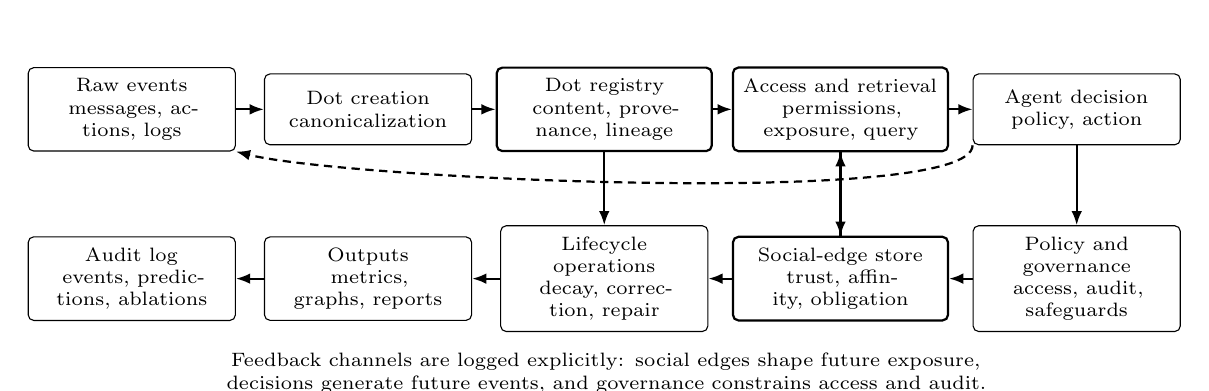
\begin{tikzpicture}[
  x=1cm,y=1cm,
  box/.style={draw, rounded corners=2pt, align=center, text width=2.35cm, minimum height=0.9cm, font=\scriptsize, inner sep=4pt},
  store/.style={draw, rounded corners=2pt, thick, align=center, text width=2.45cm, minimum height=0.95cm, font=\scriptsize, inner sep=4pt},
  arr/.style={-{Latex[length=1.8mm]}, thick},
  feed/.style={-{Latex[length=1.8mm]}, densely dashed, thick}
]
\node[box] (events) at (0,0) {Raw events\\messages, actions, logs};
\node[box] (create) at (3,0) {Dot creation\\canonicalization};
\node[store] (registry) at (6,0) {Dot registry\\content, provenance, lineage};
\node[store] (access) at (9,0) {Access and retrieval\\permissions, exposure, query};
\node[box] (decision) at (12,0) {Agent decision\\policy, action};

\node[box] (audit) at (0,-2.15) {Audit log\\events, predictions, ablations};
\node[box] (outputs) at (3,-2.15) {Outputs\\metrics, graphs, reports};
\node[box] (life) at (6,-2.15) {Lifecycle operations\\decay, correction, repair};
\node[store] (edges) at (9,-2.15) {Social-edge store\\trust, affinity, obligation};
\node[box] (govern) at (12,-2.15) {Policy and governance\\access, audit, safeguards};

\draw[arr] (events) -- (create);
\draw[arr] (create) -- (registry);
\draw[arr] (registry) -- (access);
\draw[arr] (access) -- (decision);
\draw[arr] (registry) -- (life);
\draw[arr] (access) -- (edges);
\draw[arr] (decision) -- (govern);
\draw[arr] (govern) -- (edges);
\draw[arr] (edges) -- (life);
\draw[arr] (life) -- (outputs);
\draw[arr] (outputs) -- (audit);
\draw[feed] (edges.north) -- (access.south);
\draw[feed] (decision.south west) .. controls +(0,-0.8) and +(1.4,-0.35) .. (events.south east);
\node[align=center,font=\scriptsize,text width=10.5cm] at (6,-3.35)
{Feedback channels are logged explicitly: social edges shape future exposure, decisions generate future events, and governance constrains access and audit.};
\end{tikzpicture}%
}
\caption{Executable dot-field architecture. A dot-field implementation separates event intake, dot creation, dot storage, access and retrieval, agent decisions, lifecycle operations, social-edge updates, audit logs, and governance controls. Dashed arrows denote feedback channels that must be logged rather than hidden inside an opaque memory or policy module.}
\label{fig:implementation-architecture}
\end{figure}





\subsection{Algorithmic state representation}\label{algorithmic-state-representation}

\begin{definition}[Algorithmic dot-field state]\label{def:algorithmic-dot-field-state}
An algorithmic dot-field state is a tuple
$$
\mathsf S_t=(\mathsf A,\mathsf D_t,\mathsf E_t,\mathsf R_t^D,\mathsf B_t,
\mathsf Q_t,\mathsf L_t,\mathsf I_t,\mathsf P_t,\mathsf X_t),
$$
where $\mathsf A$ is the agent registry, $\mathsf D_t$ is the dot
registry, $\mathsf E_t$ is the social-edge store, $\mathsf R_t^D$ is the
dot-relation store, $\mathsf B_t$ is the agent-dot access store,
$\mathsf Q_t$ stores effective strengths and retrieval scores,
$\mathsf L_t$ stores provenance and mutation lineages, $\mathsf I_t$ is
the institutional store, $\mathsf P_t$ is the policy and governance
layer, and $\mathsf X_t$ is the environment or task state. The
implementation is faithful to the formal theory when there is a
projection
$$
\Pi(\mathsf S_t)=(A,E_t,X_t,\bar S_t,D_t,R_t^D,B_t)=\Omega_t.
$$
\end{definition}

The algorithmic state contains more engineering detail than the formal
state. This is intentional. The formal state states what must exist for
the theory. The algorithmic state states what must be stored, indexed,
and updated by a running system.

\subsection{Dot record schema}\label{dot-record-schema}

Each dot is represented as a typed record in executable implementations. A minimal record is
$$
\begin{aligned}
\mathsf{DotRecord}(d)=(&id,x,\tau,type,origin,target,context,\\
&\sigma,\gamma,\alpha,\nu,\ell,parents,children,anchors,permissions).
\end{aligned}
$$
The fields have the following interpretation.

\begin{description}[leftmargin=3.0cm,style=nextline]
\item[$id$] A persistent identifier, such as a database key, hash, URI, or
composite identifier.
\item[$x$] Semantic content, represented as text, a symbolic proposition,
an embedding, a structured event record, or a hybrid representation.
\item[$\tau$] Creation time, observation time, or institutional write time.
\item[$type$] Dot type: observational, interactional, testimonial,
evaluative, normative, reflective, institutional, counter-dot, repair
dot, mutation, or compressed dot.
\item[$origin$] The source agent, event, artifact, institution, or process
that created the dot.
\item[$target$] The agent, group, claim, norm, institution, object, or
prior dot to which the dot refers.
\item[$context$] The task, conversation, document, location, platform,
archive, or institutional setting of creation.
\item[$\sigma,\gamma,\alpha,\nu$] Salience, credibility, affective or
normative charge, and visibility.
\item[$\ell$] Lifecycle state: active, reinforced, decayed, contested,
corrected, compressed, archived, deleted, expired, or institutionalized.
\item[$parents,children$] Lineage links for mutation, compression,
reflection, correction, or derivation.
\item[$anchors$] Canonical records, source documents, transcripts,
ledgers, policies, or institutional references used to limit drift or
verify provenance.
\item[$permissions$] Rules governing access, retention, deletion,
visibility, correction, and contestation.
\end{description}

Richer implementations may add source signatures, confidence intervals,
semantic embeddings, privacy labels, retention deadlines, extraction
confidence, institutional authority scores, and audit trails. The schema
should be modular, but content, provenance, time, access, and lifecycle
status are core.

\subsection{Stores and indexes}\label{stores-and-indexes}

Stores and indexes translate the mathematical dot field into an operational data model. The registry of dots is not enough by itself: an implementation must also maintain access indexes, target indexes, semantic indexes, lineage indexes, institutional anchors, and audit logs. These indexes are not merely engineering conveniences. They determine which traces can be retrieved efficiently, which agents can see them, which claims can be audited, and which counter-dots can be matched to target dots. A poorly indexed system may satisfy the formal ontology on paper while failing to support correction, retrieval, or validation in practice.


A scalable implementation should avoid scanning all dots for every
retrieval or edge update. The following stores form a minimal
architecture.

\begin{longtable}[]{@{}L{0.25\linewidth}L{0.34\linewidth}L{0.33\linewidth}@{}}
\toprule
\textbf{Store} & \textbf{Contents} & \textbf{Main use} \\
\midrule
\endhead
\bottomrule
\endlastfoot
Agent registry & Agent identifiers, attributes, states, policies, permissions & Action selection and access control \\
Dot registry & Dot records, lifecycle states, strengths, embeddings & Dot identity, retrieval, mutation, correction, archiving \\
Social-edge store & Typed weights such as trust, affinity, communication, authority, obligation & Transmission, influence, reputation, topology update \\
Access store & Agent-dot access relation $B_{id}(t)$, exposure logs, permissions & Determining $\mathcal M_i(t)$ and retrieval eligibility \\
Dot-relation store & Support, contradiction, causality, similarity, parenthood, compression, correction & Dot graph traversal and counter-dot discovery \\
Semantic index & Embedding or symbolic index over dot content $x(d)$ & Candidate retrieval and canonicalization \\
Target index & Map from targets to evaluative or corrective dots & Reputation, correction, edge pressure \\
Provenance index & Sources, timestamps, witnesses, archives, lineages & Auditability and identifiability \\
Institutional archive & Durable, authenticated, high-authority, or public dots & Stabilization, long-term recall, governance \\
\end{longtable}

The stores may be implemented in a graph database, relational database,
vector index, event-sourced log, or in-memory simulation object. What
matters theoretically is that the implementation preserves the three
relations $E_t$, $R_t^D$, and $B_t$ rather than collapsing them into one
undifferentiated graph.

\subsection{Reference update cycle}\label{reference-update-cycle}

A single simulation or deployment round can be implemented by the
following update cycle.

\begin{enumerate}[label=\textbf{Stage \arabic*.},leftmargin=2.2cm]
\item \textbf{Observe events.} Collect environmental observations,
messages, actions, institutional updates, retrieval logs, and social-edge
changes.
\item \textbf{Create candidate dots.} Apply $\kappa$ to events that cross
the recordability threshold.
\item \textbf{Canonicalize.} Decide whether each candidate is a new dot, a
duplicate, a mutation, a counter-dot, a repair dot, an institutional dot,
or a compressed dot.
\item \textbf{Assign provenance and access.} Attach source, time, context,
witnesses, parent dots, anchors, and initial access relations.
\item \textbf{Update dot relations.} Add support, contradiction,
causality, temporal, semantic, parenthood, compression, institutional,
and correction edges in $R_t^D$.
\item \textbf{Retrieve for agents.} For each active agent and query
$q_i(t)$, retrieve a bounded set $\mathcal V_i(q_i,t)$ of accessible, relevant,
credible, and salient dots.
\item \textbf{Act.} Agents choose actions from observations, internal
states, goals, and retrieved dots.
\item \textbf{Transmit, mutate, and compress.} Communications, summaries,
retellings, reflections, and reports create descendants or compressed
versions.
\item \textbf{Update strengths and lifecycle states.} Apply decay,
reinforcement, correction, deletion, expiration, consolidation, and
institutional stabilization.
\item \textbf{Update topology.} Use dot-induced pressure to update trust,
affinity, communication, authority, obligation, or exclusion edges.
\item \textbf{Prune or archive.} Remove, archive, or compress low-impact
dots according to governance rules while preserving required provenance
and correction rights.
\item \textbf{Log and validate.} Record provenance, access, retrieval,
mutation, action, and edge-update records; then check implementation
invariants.
\end{enumerate}

This cycle implements the theory's feedback loop:
$$
\text{events}\rightarrow\text{dots}\rightarrow\text{retrieval}\rightarrow
\text{action}\rightarrow\text{new dots}\rightarrow\text{topology update}.
$$

\subsection{Core routines}\label{core-routines}

The following routines define a minimal executable architecture.

\begin{description}[leftmargin=3.2cm,style=nextline]
\item[CreateDot$(e,c)$] Takes an event $e$ and context $c$ and returns a
candidate dot $d=\kappa(e,c)$ with content, type, provenance, initial
salience, credibility, and access rules.
\item[Canonicalize$(d,D_t)$] Searches existing dots for duplicates,
mutations, contradictions, or compression parents. It returns either a
new identifier or an update to an existing lineage.
\item[GrantAccess$(d,A,E_t,P_t)$] Updates $B_t$ using participants,
recipients, witnesses, institutional visibility, permissions, social
edges, and governance rules.
\item[Retrieve$(i,q,k)$] Returns up to $k$ dots from $\mathcal M_i(t)$ ranked by a
retrieval score such as
$$
\begin{aligned}
Score_i(d,q,t)=&\lambda_1Rel(d,q)+\lambda_2Rec(d,t)+\lambda_3\sigma_i(d,t)\\
&+\lambda_4\gamma_i(d,t)+\lambda_5Soc_i(d,t)+\lambda_6Inst(d,t).
\end{aligned}
$$
\item[Assimilate$(i,d)$] Updates the agent-specific weight, credibility,
and salience of $d$ using reinforcement, contradiction, institutional
authority, source trust, and semantic fit.
\item[Transmit$(i,j,d)$] Creates a received version $d'=T_{i\to j}(d)$,
possibly with semantic mutation, loss of context, or source relabeling.
\item[Compress$(i,S)$] Replaces or supplements a set of dots $S$ with a
compressed dot $d_S^\star=C_i(S)$ while recording the source set and the
compression rule.
\item[Correct$(c,d)$] Adds a contradiction, qualification, or defeat edge
$c\dashv d$ and updates effective counter-strength.
\item[UpdateEdges$(E_t,D_t,B_t)$] Computes edge pressure $\zeta_{ij}(t)$ and
updates social edges by a rule such as
$$
w_{ij}(t+1)=(1-\eta)w_{ij}(t)+\eta\psi(\zeta_{ij}(t)).
$$
\item[PruneArchive$(D_t,P_t)$] Applies decay thresholds, retention rules,
privacy constraints, compression policies, and archival stabilization.
\end{description}

\subsection{Implementation invariants}\label{implementation-invariants}

A valid implementation should maintain the following invariants.

\begin{enumerate}[label=(I\arabic*),leftmargin=1.3cm]
\item \textbf{Identifier uniqueness.} Every agent and dot has a unique
identifier at each time.
\item \textbf{Type consistency.} Social edges connect agents to agents;
dot-relation edges connect dots to dots; access edges connect agents to
dots.
\item \textbf{Provenance consistency.} Every non-initial dot has at least
one creation, mutation, compression, transmission, correction, or
institutionalization source.
\item \textbf{Lifecycle consistency.} A deleted or inactive dot cannot be
retrieved unless archival retrieval, leakage, or unauthorized access is
explicitly modeled.
\item \textbf{Access consistency.} Retrieval by agent $a_i$ is limited to
dots accessible to $a_i$, except in experimental or counterfactual query
modes.
\item \textbf{Weight bounds.} Salience, credibility, visibility,
retrievable strength, valence, and edge weights remain in their declared
domains.
\item \textbf{Relation validity.} Every dot relation has an admissible type,
such as support, contradiction, temporal precedence, causation, mutation,
compression, institutional reference, repair, or semantic similarity.
\item \textbf{Lineage acyclicity.} Parent-child mutation and compression
relations are acyclic unless iterative revision is explicitly represented
by time-indexed versions.
\item \textbf{Institutional anchor consistency.} Institutional dots record
anchor, authority, timestamp, and access rule, or explicitly declare those
fields latent.
\end{enumerate}

\begin{theorem}[Validity preservation by typed update]\label{thm:validity-preservation-typed-update}
Suppose $\mathsf S_t$ is a valid algorithmic dot-field state. Suppose
each implementation routine is type preserving, respects declared weight
bounds, records required provenance, updates access only through
admissible access rules, and creates only admissible relation edges. Then
the reference update cycle produces a valid algorithmic dot-field state
$\mathsf S_{t+1}$.
\end{theorem}

\begin{proof}
The proof is by induction over the update cycle. Dot creation generates
candidate records with required fields. Canonicalization either maps a
candidate to an existing dot or creates a new identifier, preserving
identifier uniqueness. Relation updates add only typed admissible edges,
preserving type consistency and relation validity. Access updates modify
only agent-dot relations under declared rules, preserving access
consistency. Retrieval is restricted to accessible dots by assumption.
Assimilation changes strengths and lifecycle states only through bounded
operators. Mutation and compression add parent-child lineage links under
a time-ordering or acyclicity rule. Institutionalization records anchors
and authority metadata. Topology updates alter only agent-agent edge
stores and keep weights within declared bounds. Thus every invariant
holds at $t+1$.
\end{proof}

\subsection{Implementation soundness}\label{implementation-soundness}

\begin{definition}[Implementation of a dot-field kernel]\label{def:kernel-implementation}
Let $\mathsf K$ be a formal transition kernel over valid dot fields. An
algorithm $\mathcal A$ exactly implements $\mathsf K$ if, for every valid
$\Omega_t$ and measurable set $C$,
$$
P_{\mathcal A}(\Pi(\mathsf S_{t+1})\in C\mid \Pi(\mathsf S_t)=\Omega_t)
=\mathsf K(C\mid \Omega_t).
$$
It $\varepsilon$-implements $\mathsf K$ under divergence $\mathsf D$ if
$$
\mathsf D\left(P_{\mathcal A}(\Pi(\mathsf S_{t+1})\mid\Omega_t),
\mathsf K(\cdot\mid\Omega_t)\right)\leq\varepsilon
$$
for all valid $\Omega_t$ in the evaluated state class.
\end{definition}

\begin{theorem}[Executable Markov-kernel realization]\label{thm:executable-markov-kernel-realization}
Assume the implementation routines in the reference cycle condition only
on the current algorithmic state $\mathsf S_t$, current exogenous inputs
$\xi_t$, and random seeds independent of the past given $\mathsf S_t$.
Then the executable process defines a Markov kernel over algorithmic
dot-field states. If each routine exactly implements its corresponding
formal operator, then the projected process realizes the formal
Dot-Trace transition kernel. If each routine implements its operator with
bounded one-step divergence and the composition of routines is stable
under that divergence, then the executable process is an approximate
implementation of the formal kernel.
\end{theorem}

\begin{proof}
The next state is generated by a finite composition of routine outputs.
By assumption, every routine receives only $\mathsf S_t$, current
exogenous inputs, and conditionally independent randomness. Therefore the
conditional distribution of $\mathsf S_{t+1}$ depends on the past only
through $\mathsf S_t$, which defines a Markov kernel. If each routine is
identical to the corresponding formal operator under projection $\Pi$,
the composition is identical to the formal transition kernel. With
approximate routines, bounded one-step divergence propagates through the
finite composition according to the stability property of the chosen
divergence.
\end{proof}

This theorem connects the implementation to Section~\ref{dot-field-markov-restoration}.
The formal theory says that transition-relevant history must be carried
by the current dot field. The implementation theorem says that a program
which uses only that represented state can realize a Markov dot-field
simulator.

\subsection{Approximate retrieval and bounded memory}\label{approximate-retrieval-and-bounded-memory}

Exact retrieval may be infeasible when many agents and dots exist. An
implementation therefore needs approximation guarantees.

\begin{definition}[Retrieval feature map]\label{def:retrieval-feature-map}
For a retrieved set $\mathcal V_i(q,t)$, define
$$
h_i(\mathcal V_i)=\sum_{d\in \mathcal V_i(q,t)}Q_i(d,t)\varphi(d),
$$
where $Q_i(d,t)$ is effective retrievable strength and $\varphi(d)$ is a
semantic, symbolic, or task-specific feature vector. A policy is
$L_\pi$-Lipschitz in retrieval features if
$$
\|\pi_i(\cdot\mid o,s,h)-\pi_i(\cdot\mid o,s,h')\|_{TV}
\leq L_\pi\|h-h'\|
$$
for all admissible $o,s,h,h'$.
\end{definition}

\begin{proposition}[Approximate retrieval action bound]\label{prop:approximate-retrieval-action-bound}
Let $R_i$ be the exact retrieved set and $\widetilde R_i$ an approximate
retrieved set for the same query. If
$$
\|h_i(\mathcal V_i)-h_i(\widetilde R_i)\|\leq\varepsilon,
$$
and the policy is $L_\pi$-Lipschitz in retrieval features, then
$$
\|\pi_i(\cdot\mid o_i,s_i,h_i(\mathcal V_i))-\pi_i(\cdot\mid o_i,s_i,h_i(\widetilde R_i))\|_{TV}
\leq L_\pi\varepsilon.
$$
\end{proposition}

\begin{proof}
The result follows by substituting the feature-error bound into the
Lipschitz condition.
\end{proof}

\begin{proposition}[Bounded-memory truncation error]\label{prop:bounded-memory-truncation-error}
Suppose an implementation ignores, archives, or drops a set of dots
$G_i(t)$ for agent $a_i$, and suppose the omitted feature mass satisfies
$$
\left\|\sum_{d\in G_i(t)}Q_i(d,t)\varphi(d)\right\|\leq\epsilon_i(t).
$$
If $\pi_i$ is $L_\pi$-Lipschitz in retrieval features, then the action
distribution induced by the truncated memory differs from the full-memory
action distribution by at most $L_\pi\epsilon_i(t)$ in total variation.
\end{proposition}

\begin{proof}
The feature vector contributed by omitted dots has norm at most
$\epsilon_i(t)$. Thus the difference between full and truncated retrieval
features is at most $\epsilon_i(t)$. Applying the Lipschitz condition
gives the bound.
\end{proof}

The truncation result provides a principled route to bounded memory. A
system need not keep every low-impact trace active forever. It must
preserve, approximate, or archive enough transition-relevant dot mass to
keep action, correction, and topology errors within a declared tolerance.

\subsection{Complexity bounds}\label{complexity-bounds}

Let $n=|A|$, $m=|D_t|$, $e_A=|E_t|$, $e_D=|R_t^D|$, and $b=|B_t|$. Let
$k$ be the maximum number of retrieved dots per agent, $p$ the semantic
feature dimension, $c$ the number of indexed candidates scored per
agent, $K$ the size of a fixed dot vocabulary in consensus updates, and
$|Ev_t|$ the number of events in the current batch.

\begin{proposition}[Sparse implementation complexity]\label{prop:sparse-implementation-complexity}
Under sparse storage, one update step can be implemented with memory
$$
O(n+m+e_A+e_D+b+|\mathsf I_t|).
$$
Exact retrieval by scanning every accessible dot costs
$$
O\left(\sum_{i=1}^n |\mathcal M_i(t)|p\right)
$$
for score computation, plus top-$k$ selection. Indexed retrieval that
returns $c$ candidates per agent costs $O(ncp)$ plus index-query
overhead. Dot-consensus updates over a fixed vocabulary of size $K$ cost
$O(e_AK)$ under sparse social influence. Edge updates based only on
retrieved evaluative dots cost $O(nk)$ to aggregate pressures, plus the
cost of writing changed edges.
\end{proposition}

\begin{proof}
The memory bound follows by storing each table and sparse edge set once.
Exact retrieval scores each accessible agent-dot pair, producing the sum
over $|\mathcal M_i(t)|$ with feature dimension $p$. Candidate retrieval scores
only $c$ candidates for each of $n$ agents. Sparse consensus multiplies
each nonzero social-influence edge by a length-$K$ vector, giving
$O(e_AK)$. If each agent acts on at most $k$ retrieved evaluative dots,
pressure aggregation visits at most $nk$ retrieved dot instances.
\end{proof}

\begin{remark}[Computational design principle]
Dense representations are useful for proofs, but realistic
implementations should be sparse, indexed, and event driven. Dot-Trace
Theory should not be implemented as an all-agents by all-dots dense
matrix unless the population and dot vocabulary are small.
\end{remark}

\subsection{Reference implementation outputs}\label{reference-implementation-outputs}

A reference implementation should produce outputs at three levels. The first level is the transition log: for each time step it records observed events, created dots, granted access, retrieved dots, action probabilities, realized actions, corrections, mutations, and edge updates. The second level is the state snapshot: it records the dot registry, access relation, social graph, dot graph, memory weights, institutional anchors, and correction state. The third level is the evaluation report: it records baseline comparisons, ablations, prediction lift, extraction quality, and any failed invariants.

These outputs matter because Dot-Trace Theory is otherwise difficult to audit. A plausible agent conversation is not enough. The implementation must be able to answer why a dot was created, who could access it, whether it was retrieved, how it affected a decision, whether it mutated, and whether it changed the topology through which later dots traveled. Without these records, the implementation may simulate trace-mediated behavior, but it cannot support a scientific claim about trace-mediated mechanisms.


A minimal implementation should report $\widehat\Omega_t$, created dots,
retrieved dots, action choices, mutation and compression events,
institutional writes, edge updates, correction states, invariant
violations, runtime, memory use, and prediction lift relative to a
baseline. In simulation, it should also record ground-truth latent
quantities so that reconstruction, identifiability, and approximation
error can be evaluated.

\begin{remark}[Implementation as theory test]
An executable architecture makes Dot-Trace Theory falsifiable. If
dot-field models fail to outperform agent-edge or flat-memory baselines
under fair validation, the theory's practical value is weakened. If they
improve prediction, coordination, correction, auditability, and
social-memory control, the theory gains empirical support.
\end{remark}

\section{Minimal Executable Simulator Specification}\label{minimal-executable-simulator-specification}

The algorithmic implementation section identifies the computational
objects needed by Dot-Trace Theory. This section makes the proposal more
operational by specifying a minimal executable simulator. The simulator
is intentionally small. It is not meant to reproduce all human social
complexity. Its purpose is to provide a reference environment in which
core claims of the theory can be tested, falsified, debugged, and
extended.

The simulator should satisfy five design requirements.

\begin{enumerate}[leftmargin=*]
\item It must explicitly represent agents, dots, agent-agent edges,
agent-dot access relations, and dot-dot relations.
\item It must implement the full trace loop: interaction creates dots;
dots are retrieved; retrieved dots affect action; action creates new
dots; dots modify social edges; social edges control future dot
exposure.
\item It must be inspectable. Every created dot, retrieved dot,
transmission, mutation, correction, and edge update should be logged.
\item It must support baselines that remove parts of the dot field so the
additional value of dot structure can be tested.
\item It must be reproducible under a fixed seed and configuration file.
\end{enumerate}

\subsection{Simulator objective}\label{simulator-objective}

The minimal simulator is designed to answer a precise question:

\begin{quote}
When does an explicit dot field explain, predict, or control social
multi-agent behavior better than an agent-edge model or a flat-memory
model?
\end{quote}

It therefore treats the dot field not as decoration but as the object of
experimental manipulation. A simulation run should make it possible to
compare the following model classes.

\begin{description}[leftmargin=3.2cm,style=nextline]
\item[Edge-only baseline]
Agents have social edges and current observations, but no explicit dot
memory. Predictions depend on $E_t$ and $X_t$ only.

\item[Flat-memory baseline]
Agents store private memories but there is no dot-dot graph, provenance,
access graph, mutation lineage, institutional archive, or topology
feedback.

\item[Dot-field model]
Agents act through retrieved dots, dots have provenance and lifecycle
states, access is represented explicitly, and social edges update from
dot-induced pressure.

\item[Full dot-field model]
The dot-field model is augmented with mutation, compression,
counter-dots, institutional anchors, and logging sufficient for
identifiability analysis.
\end{description}

The theory gains empirical support when the dot-field model produces
better out-of-sample prediction, lower reconstruction error, better
coordination control, faster correction, or more faithful recovery of
known simulated mechanisms than the baselines.

\subsection{Minimal simulator state}\label{minimal-simulator-state}

A minimal simulation state at time $t$ is
$$
\mathcal S_t^{sim}=(A,D_t,W_t,B_t,R_t^D,M_t,L_t,C_t,X_t),
$$
where $A$ is a finite set of agents, $D_t$ is the dot registry, $W_t$ is
the weighted social adjacency matrix, $B_t$ is the access relation,
$R_t^D$ is the dot-dot relation set, $M_t$ stores agent-specific dot
weights, $L_t$ stores lineages and provenance, $C_t$ stores correction
states, and $X_t$ is the environment or task state.

The smallest useful simulator can use the following simplifications.

\begin{enumerate}[leftmargin=*]
\item Each dot has a target agent or target issue.
\item Each dot has scalar valence $v(d)\in[-1,1]$.
\item Each dot has a scalar credibility $\gamma(d)\in[0,1]$.
\item Each agent-dot pair has a memory weight $m_i(d,t)\in[0,1]$.
\item Social edges are trust or communication weights
$w_{ij}(t)\in[0,1]$.
\item Dot retrieval is top-$k$ retrieval by a weighted score.
\item Dot transmission occurs with probability increasing in
$w_{ij}(t)$.
\end{enumerate}

These simplifications retain the essential loop while keeping the first
implementation small enough to inspect manually.


Figure~\ref{fig:minimal-simulator-loop} shows the minimal simulator loop. The simulator is useful only if the same event log can be evaluated under multiple representations. The edge-only baseline observes social weights but ignores dots. The private-memory baseline stores agent-specific memories but removes social access and provenance. The full dot-field condition retains access, retrieval, lineage, mutation, correction, and topology feedback.

\begin{figure}[htbp]
\centering
\resizebox{0.94\textwidth}{!}{%
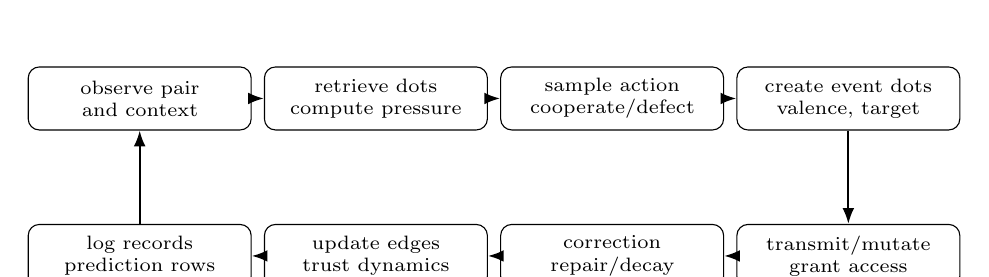
\begin{tikzpicture}[
  x=1cm,y=1cm,
  box/.style={draw, rounded corners, align=center, text width=2.55cm, minimum height=0.8cm, font=\scriptsize, inner sep=4pt},
  arr/.style={-{Latex[length=2mm]}, thick}
]
\node[box] (observe) at (0,0) {observe pair\\and context};
\node[box] (retrieve) at (3.0,0) {retrieve dots\\compute pressure};
\node[box] (act) at (6.0,0) {sample action\\cooperate/defect};
\node[box] (create) at (9.0,0) {create event dots\\valence, target};
\node[box] (spread) at (9.0,-2.0) {transmit/mutate\\grant access};
\node[box] (correct) at (6.0,-2.0) {correction\\repair/decay};
\node[box] (edges) at (3.0,-2.0) {update edges\\trust dynamics};
\node[box] (log) at (0,-2.0) {log records\\prediction rows};
\draw[arr] (observe) -- (retrieve); \draw[arr] (retrieve) -- (act); \draw[arr] (act) -- (create); \draw[arr] (create) -- (spread);
\draw[arr] (spread) -- (correct); \draw[arr] (correct) -- (edges); \draw[arr] (edges) -- (log); \draw[arr] (log) -- (observe);
\end{tikzpicture}%
}
\caption{Minimal simulator loop. The simulator is a restricted executable realization of the dot-field transition: retrieve traces, act, create traces, transmit and mutate them, apply correction and decay, update social edges, and log the transition for validation.}
\label{fig:minimal-simulator-loop}
\end{figure}


\subsection{Parameter set}\label{minimal-parameter-set}

The parameter set should be organized by mechanism rather than listed as an undifferentiated vector. Memory parameters control decay, reinforcement, retrieval depth, and salience. Transmission parameters control whether a dot crosses an agent-agent edge and whether it mutates. Correction parameters control counter-dot strength, semantic fit, and repair probability. Topology parameters control how retrieved evaluative dots change social edges. Institutional parameters control reach, persistence, authority, and archival access. Grouping parameters in this way makes ablation interpretable: when a result changes, the researcher can identify which theoretical mechanism was changed.


A minimal configuration is
$$
\Theta^{sim}=\{n,T,k,\lambda_m,\eta_w,p_0,p_I,p_C,\beta_\zeta,\beta_W,\epsilon_\mu,\rho_C,\tau\}.
$$
The parameters are interpreted as follows.

\begin{longtable}{L{0.18\textwidth}L{0.70\textwidth}}
\toprule
Parameter & Interpretation \\
\midrule
$n$ & Number of agents. \\
$T$ & Number of simulation periods. \\
$k$ & Number of dots retrieved per agent-decision. \\
$\lambda_m$ & Private dot-retention factor. \\
$\eta_w$ & Social-edge learning rate. \\
$p_0$ & Baseline probability of dot transmission. \\
$p_I$ & Probability that a new dot is institutionalized or archived. \\
$p_C$ & Probability that a counter-dot is generated after detecting error. \\
$\beta_\zeta$ & Action sensitivity to dot-induced pressure. \\
$\beta_W$ & Action sensitivity to current social-edge weight. \\
$\epsilon_\mu$ & Maximum or standard deviation of mutation noise. \\
$\rho_C$ & Corrective strength of a counter-dot. \\
$\tau$ & Edge threshold for observed tie formation. \\
\bottomrule
\end{longtable}

The first implementation should keep $\Theta^{sim}$ small. A large
parameter space can obscure the causal mechanisms that the simulator is
supposed to expose.

\subsection{Dot record for the minimal simulator}\label{minimal-dot-record}

The minimal simulator record deliberately uses a small number of fields, but those fields are chosen to preserve the essential theoretical distinctions. Content and valence determine what the dot says. Origin and target determine provenance and direction. Credibility and memory weight determine effective strength. Parent links preserve lineage for mutation, compression, and correction. Anchor status distinguishes private traces from institutional traces. Even in a small simulator, omitting these fields makes it difficult to test whether an outcome was produced by memory, topology, credibility, access, or institutional persistence.


A minimal dot record is
$$
\mathsf d=(id,origin,target,type,x,v,\gamma,\tau,parents,status,anchor),
$$
where $x$ is semantic content or an embedding, $v$ is valence, $\gamma$
is credibility, $\tau$ is creation time, $parents$ records provenance,
$status$ records lifecycle state, and $anchor$ indicates whether the dot
is institutionally anchored.

For a first simulation, $x$ may be a scalar issue coordinate or a low
-dimensional vector. Later implementations can replace $x$ with text,
embeddings, symbolic claims, or graph-structured content.

\subsection{Retrieval rule}\label{minimal-retrieval-rule}

Retrieval is the mechanism through which stored dots become behaviorally active. The simulator should therefore separate accessible dots from retrieved dots. A dot may exist and be accessible without entering the current decision context. Conversely, a high-salience or high-credibility dot may dominate action even when many other dots are available. The retrieval rule should report both the selected top-$k$ dots and the score components that produced the ranking; otherwise, later prediction and audit steps cannot distinguish relevance effects from credibility, recency, or social-source effects.


Agent $a_i$ retrieves dots relevant to a query $q$ using
$$
s_i(d,q,t)=
\omega_R Rel(d,q)+\omega_M m_i(d,t)+\omega_C\gamma_i(d,t)
+\omega_T Rec(d,t)+\omega_S Soc_i(d,t),
$$
where $Rel$ is semantic relevance, $m_i$ is memory weight, $\gamma_i$ is
credibility, $Rec$ is recency, and $Soc_i$ is social-source weight. The
retrieved set is
$$
\mathcal V_i(q,t)=\operatorname{TopK}_{d\in \mathcal M_i(t)}s_i(d,q,t).
$$
The simulator should log not only $\mathcal V_i(q,t)$ but also the
candidate scores. This is needed to diagnose whether behavior changed
because of the dot field, the retrieval rule, or the action rule.

\subsection{Action rule}\label{minimal-action-rule}

The action rule is the point at which the dot field affects behavior. A useful simulator should expose both reduced and dot-augmented action probabilities for the same event. This permits row-level prediction-lift analysis: the researcher can ask whether access to retrieved dot pressure improves prediction of the observed action relative to edge-only or flat-memory predictors. The action rule should also allow stochasticity, because deterministic policies can conceal uncertainty and make validation too dependent on threshold choices.


For pairwise cooperation, agent $a_i$ decides whether to cooperate with
agent $a_j$. Define dot pressure toward $a_j$ as
$$
\zeta_{ij}(t)=\sum_{d\in \mathcal V_i(q_{ij},t):T(d)=a_j}
 m_i(d,t)\gamma_i(d,t)v_i(d,j,t).
$$
The cooperation probability is
$$
P_i(C\mid j,t)=
\sigma\left(b_i+\beta_W w_{ij}(t)+\beta_\zeta \zeta_{ij}(t)\right),
$$
where $\sigma(x)=1/(1+e^{-x})$. This implements the central claim that
current edge weight and retrievable traces jointly shape action.

A competing edge-only baseline uses
$$
P_i^{edge}(C\mid j,t)=\sigma(b_i+\beta_W w_{ij}(t)),
$$
while a flat-memory baseline may use private memory weights but ignore
provenance, dot-dot relations, mutation, access, and social transmission.

\subsection{Dot creation rule}\label{minimal-dot-creation-rule}

Dot creation should be event-sensitive. Cooperation, defection, promise keeping, promise breaking, correction, apology, sanction, endorsement, and institutional recording should not all create identical traces. Each event should create dots with target, valence, provenance, credibility, and lifecycle status appropriate to the event. This is where the simulator encodes the claim that social action leaves trace structure rather than merely changing an edge weight.


Actions create evaluative dots. If $a_i$ cooperates with $a_j$, then
$a_j$ may receive a positive dot about $a_i$:
$$
d^+_{i\to j,t}=\text{``}a_i\text{ cooperated with }a_j\text{ at }t\text{''},
\qquad v(d^+)>0.
$$
If $a_i$ defects against $a_j$, then $a_j$ may receive a negative dot:
$$
d^-_{i\to j,t}=\text{``}a_i\text{ defected against }a_j\text{ at }t\text{''},
\qquad v(d^-)<0.
$$
The dot is added to $D_{t+1}$, the creator receives access, and the
lineage log records the triggering event. In an institutional condition,
the dot may also be written to an archive with probability $p_I$.

\subsection{Transmission and access rule}\label{transmission-and-access-rule}

Transmission and access are distinct. Transmission concerns the movement or reproduction of a dot from one location to another. Access concerns whether a given agent can later retrieve or encounter it. A dot can be transmitted publicly but ignored by an agent, or transmitted privately but become institutionally discoverable later. The simulator should therefore record both the transmission event and the resulting access relation. This distinction is necessary for modeling rumors, archives, permissioned records, bridge ties, and correction failures.


If agent $a_i$ has access to dot $d$ and communicates with $a_j$, then
$a_j$ receives access to a descendant dot $d'$ with probability
$$
P((a_j,d')\in B_{t+1})=p_0 w_{ij}(t)\gamma_i(d,t).
$$
If mutation is disabled, $d'=d$. If mutation is enabled,
$$
d'=T_{i\to j}(d),
\qquad
x(d')=x(d)+\xi_{ij,t},
$$
where $\xi_{ij,t}$ is bounded or mean-zero mutation noise. The lineage
store records $d\to d'$.

This rule allows the simulator to distinguish transmission failure,
access failure, credibility failure, and mutation-induced distortion.

\subsection{Lifecycle and decay rule}\label{minimal-lifecycle-decay-rule}

Decay should not be interpreted as simple deletion. A dot may lose salience while remaining accessible, remain in an archive while becoming practically invisible, or persist institutionally while losing credibility. The lifecycle rule should therefore update memory weight, credibility, visibility, and status separately when possible. This allows the simulator to represent dormant records, stale reputations, corrected accusations, and institutional traces that persist despite reduced behavioral force.


For every accessible dot,
$$
m_i(d,t+1)=\lambda_m m_i(d,t)+r_i(d,t)-c_i(d,t),
$$
clipped to $[0,1]$, where $r_i(d,t)$ is reinforcement from retrieval,
repetition, institutional anchoring, or successful action, and
$c_i(d,t)$ is correction or suppression. A simple default is
$$
r_i(d,t)=\rho_R\mathbf 1\{d\in\mathcal V_i(q,t)\}
+\rho_I\mathbf 1\{d\text{ is anchored}\}.
$$
Institutional dots can be implemented with a larger retention factor
$\lambda_I>\lambda_m$ or with recurring reinforcement $\rho_I>0$.

\subsection{Social-edge update rule}\label{minimal-social-edge-update-rule}

The edge-update rule is the minimal simulator's topology-feedback mechanism. It should compute edge pressure from retrieved evaluative dots rather than from all stored dots. This preserves the theory's distinction between what an agent could know and what an agent actually uses in a decision. Edge updates should also be bounded and inertial, because trust, affiliation, and communication ties typically change gradually except under high-salience shocks.


After action and retrieval, social edges update by dot-induced pressure:
$$
w_{ij}(t+1)=
(1-\eta_w)w_{ij}(t)+\eta_w\sigma(\alpha_0+\alpha_\zeta \zeta_{ij}(t)).
$$
The observed thresholded graph is
$$
E_t^\tau=\{(i,j):w_{ij}(t)>\tau\}.
$$
This equation links individual memory to social topology. Positive
retrieved dots can create or strengthen ties; negative retrieved dots
can weaken or remove ties.

\subsection{Counter-dot and repair rule}\label{minimal-counter-dot-rule}

The simulator should distinguish factual correction from social repair. A counter-dot can reduce the active error associated with a false or obsolete trace, but the social edge damaged by the original trace may not recover automatically. Repair requires additional positive dot pressure, renewed access, apology, institutional rectification, or repeated cooperative interaction. This distinction is essential for modeling residual harm after false accusations, failed retractions, and reputational recovery.


A counter-dot $c\dashv d$ is generated when an error signal or external
intervention indicates that target dot $d$ is false, obsolete,
misleading, or socially harmful. The counter-dot reduces active support
when it is accessible, retrieved, credible, and semantically fitted:
$$
CE_i(c,d,t)=Q_i(c,t)\kappa_i(c,d,t).
$$
A minimal correction update is
$$
e_i(d,t+1)=\left[\lambda_e e_i(d,t)+L_i(d,t)-CE_i(c,d,t)\right]_+.
$$
If the dot has already damaged a social edge, a separate repair dot may
be required. The simulator should therefore log both factual correction
and edge repair.

\subsection{Simulation loop}\label{minimal-simulation-loop}

The reference transition from $\mathcal S_t^{sim}$ to
$\mathcal S_{t+1}^{sim}$ is:

\begin{enumerate}[leftmargin=*]
\item sample interaction pairs or communication events;
\item for each decision, retrieve top-$k$ relevant dots;
\item compute dot pressure and action probabilities;
\item sample actions;
\item create new dots from observed actions;
\item transmit dots along communication edges;
\item mutate transmitted dots when mutation is enabled;
\item generate counter-dots or repair dots when correction conditions are met;
\item update dot weights, lifecycle states, and institutional archives;
\item update social edges from dot-induced pressure;
\item compute metrics and write an auditable event log.
\end{enumerate}

In pseudocode:

\begin{verbatim}
Initialize agents A, social weights W, empty dot registry D, access B
For t = 0,...,T-1:
    pairs = sample_interactions(A, W, X)
    For each ordered pair (i,j) in pairs:
        R_i = retrieve(i, query_about(j), D, B, M, W)
        \zeta_ij = aggregate_pressure(i, j, R_i)
        action_i = sample_action(i, j, W[i,j], \zeta_ij)
        new_dots = create_dots(action_i, i, j, t)
        add new_dots to D, B, L
    For each communication edge (i,j):
        transmit accessible dots from i to j with probability p0*W[i,j]
        apply mutation if enabled and record lineage
    Generate counter-dots and repair dots if correction triggers fire
    Update dot weights, decay, reinforcement, anchors, and statuses
    Update social weights W using dot-induced pressure
    Log state, events, retrievals, created dots, transmissions, and metrics
Return logs and final dot field
\end{verbatim}

\subsection{Reference experimental conditions}\label{reference-experimental-conditions}

Experimental conditions should be chosen to isolate mechanisms rather than to demonstrate only the full model. A useful design includes at least one condition that activates each mechanism and one matched condition that removes it. For example, mutation can be tested by comparing exact transmission with noisy transmission; institutional stabilization can be tested by comparing private-only traces with archived traces; correction can be tested by varying counter-dot reach; and topology feedback can be tested by freezing social edges after the initial graph.


A useful first simulator should include at least eight experimental
conditions.

\begin{enumerate}[leftmargin=*]
\item \textbf{No-dot baseline:} agents update edges from actions only.
\item \textbf{Private-dot condition:} agents remember only their own dots.
\item \textbf{Social-transmission condition:} dots transmit across social
edges.
\item \textbf{Consensus condition:} connected agents repeatedly exchange
dot weights.
\item \textbf{Fragmentation condition:} two or more weakly connected
clusters exchange dots internally but not externally.
\item \textbf{Mutation condition:} transmitted dots drift semantically.
\item \textbf{Institutional condition:} selected dots are archived with
higher persistence and broader reach.
\item \textbf{Correction condition:} counter-dots and repair dots are
introduced at controlled times.
\end{enumerate}

Each condition is compared against edge-only and flat-memory baselines using the same random seeds when possible.

\subsection{Validation tests mapped to theorems}\label{validation-tests-mapped-to-theorems}

The simulator is useful only if each run is interpretable as a test of a stated mechanism. For that reason, validation tasks are mapped to theorem signatures rather than to arbitrary software features. A consensus benchmark should test convergence of dot weights; a sequencing benchmark should test non-commutativity; an institutional benchmark should test persistence and correction cost; a topology benchmark should test dot-induced edge change. This mapping prevents a simulation from becoming a demonstration of plausibility without a clear theoretical target.


The simulator is used to test theorem signatures rather than merely to produce plausible behavior. Table~\ref{tab:simulator-theorem-tests}
maps theoretical claims to executable tests.

\begin{longtable}{L{0.31\textwidth}L{0.57\textwidth}}
\caption{Minimal simulator validation tests.}\label{tab:simulator-theorem-tests}\\
\toprule
Theoretical component & Simulator test \\
\midrule
Representational insufficiency & Construct two runs with identical
$W_t$ and observations but different accessible dots; verify divergent
actions. \\
Dot-field Markov restoration & Show that prediction improves when the
current dot field is included as state, relative to history-free edge
projection. \\
Dot consensus & Run connected exchange with fixed vocabulary; verify
convergence of dot-weight vectors. \\
Fragmented memory & Run block-separated clusters; verify separate
component barycenters and nonzero fragmentation index. \\
Temporal sequencing & Expose agents to the same dots in different
orders; verify different final memory or edge states. \\
Institutional stabilization & Compare private and archived dots; verify
longer half-life, larger reach, and higher correction cost for archived
dots. \\
Dot-induced topology & Let edges update from evaluative dots; verify
formation, removal, exclusion, reputation, and alliance dynamics. \\
Counter-dot correction & Introduce counter-dots at controlled strength
and reach; verify correction thresholds and residual topology harm. \\
Mutation and compression & Transmit dots over multiple hops and compress
dot sets; verify drift, behavioral compression loss, and correction
mismatch. \\
Identifiability & Hide or reveal logs; verify which dot-field quantities
can be recovered under each observability regime. \\
\bottomrule
\end{longtable}

\subsection{Logging and audit format}\label{logging-and-audit-format}

A transition log should be structured enough to reconstruct the causal chain claimed by the theory. At minimum, each row should include time, acting agent, target agent or issue, accessible dots, retrieved dots, action probability, realized action, created dots, transmitted dots, mutations, corrections, edge update, and random seed. The log is not merely an implementation convenience; it is the evidence that the simulator instantiated the formal mechanism under analysis.


Every transition should produce an append-only log. A minimal event log
entry is
$$
\ell_t=(time,event\_type,actors,dots,parents,action,old\_state,new\_state,seed).
$$
The simulator should log at least the following event types:

\begin{enumerate}[leftmargin=*]
\item interaction sampled;
\item dots retrieved;
\item action sampled;
\item dot created;
\item dot transmitted;
\item dot mutated;
\item dot compressed;
\item dot institutionalized;
\item counter-dot generated;
\item repair dot generated;
\item memory weight updated;
\item social edge updated;
\item invariant violation detected.
\end{enumerate}

The log is not merely an engineering artifact. It is part of the
scientific design. Without logs, dot-field mechanisms cannot be audited,
identified, or compared against simpler baselines.

\subsection{Minimal simulator outputs}\label{minimal-simulator-outputs}

The minimal outputs should be interpretable without reading source code. A final report should state the number of agents, dots, edges, access relations, transmitted dots, corrected dots, institutional dots, and mutations. It should also report prediction lift, fragmentation, correction latency, reputation volatility, and topology-memory coupling. These summaries allow the simulator to serve as a benchmark rather than only as an illustrative demonstration.


Each run should return:

\begin{enumerate}[leftmargin=*]
\item final social graph $W_T$ and thresholded graph $E_T^\tau$;
\item final dot registry $D_T$;
\item final access relation $B_T$;
\item final dot-weight matrix $M_T$;
\item dot creation, transmission, mutation, correction, and archive logs;
\item coordination rate, cooperation rate, and payoff summaries;
\item collective memory convergence and fragmentation scores;
\item reputation and exclusion-risk trajectories;
\item correction latency and residual topology harm;
\item prediction lift over baselines.
\end{enumerate}

\subsection{Reference hypotheses for the simulator}\label{reference-hypotheses-simulator}

The simulator hypotheses should be stated before runs are inspected. For example, when retrieval is memory-sensitive, dot-field predictors should outperform edge-only predictors. When clusters have weak bridges, fragmentation should persist over finite horizons. When counter-dot reach is low, correction should fail even if the counter-dot exists globally. When institutional persistence is high, institutional dots should dominate private dots in retrievable strength. Prespecifying these signatures keeps the simulator from becoming a post hoc storytelling tool.


A reference simulator tests the following specific hypotheses.

\begin{description}[leftmargin=2.5cm,style=nextline]
\item[S1] Dot-field agents predict partner behavior better than edge-only
agents when the environment contains memory-sensitive interactions.

\item[S2] Dot transmission increases collective memory convergence in
connected graphs but increases fragmentation in clustered graphs when
cross-cluster bridges are weak.

\item[S3] Institutional archives increase coordination when archived dots
are accurate and increase correction cost when archived dots are false or
obsolete.

\item[S4] Semantic mutation increases correction latency because
counter-dots lose fit with mutated descendants.

\item[S5] Provenance-rich logs improve reconstruction of dot-induced
edge pressure and reduce ambiguity in post-hoc explanation.
\end{description}

\subsection{Minimal Python architecture}\label{minimal-python-architecture}

The minimal Python architecture should mirror the formal hierarchy. Agent objects should not store all social state internally; otherwise, access and topology become difficult to audit. Dot objects should not be reduced to text strings; otherwise, provenance, credibility, lifecycle, and lineage disappear. The simulator state should own the registries, edge matrices, access sets, and logs so that the whole transition can be serialized, replayed, and compared across ablations.


A compact Python implementation should have four classes:

\begin{description}[leftmargin=2.8cm,style=nextline]
\item[Agent]
Stores agent id, bias, policy parameters, and optional role or group.

\item[Dot]
Stores dot id, origin, target, type, valence, credibility, semantic
content, timestamp, parent ids, anchor state, and lifecycle status.

\item[DotTraceState]
Stores agents, dots, social weights, access sets, memory weights,
relations, lineage, correction states, and logs.

\item[DotTraceSimulator]
Stores configuration, random seed, transition routines, metrics, and the
main run loop.
\end{description}

The implementation should avoid hidden global variables. All randomness
should pass through an explicit pseudo-random number generator. This
makes simulation runs reproducible and allows theorem-specific test cases
to be replayed exactly.

\subsection{Reproducibility checklist}\label{reproducibility-checklist}

A checklist should also distinguish reproducibility from repeatability. Repeatability means that the same code and seed reproduce the same trajectory. Reproducibility means that another researcher can understand the assumptions, reconstruct the condition, and obtain comparable signatures under independent implementation choices. The checklist should therefore include the conceptual condition, active mechanisms, data-generation process, randomization scheme, and validation outputs, not only code dependencies.


Reproducibility requires more than a random seed. The report should record parameter values, graph initialization, dot initialization, baseline condition, enabled mechanisms, software version, and output schema. It should also record whether the run used oracle probabilities, fitted predictors, or held-out evaluation. Without these details, simulation results cannot be compared across revisions or reused by independent researchers.


A run is reproducible when it reports:

\begin{enumerate}[leftmargin=*]
\item simulator version;
\item configuration parameters;
\item random seed;
\item initial graph and initial dots;
\item update-rule choices;
\item enabled and disabled mechanisms;
\item baseline definitions;
\item full event log or a hash of the event log;
\item metric definitions;
\item code commit or file checksum.
\end{enumerate}

\subsection{Minimal simulator theorem}\label{minimal-simulator-theorem}

\begin{theorem}[Simulator faithfulness under projection]\label{thm:simulator-faithfulness-projection}
Let $\mathcal S_t^{sim}$ be a minimal simulator state with projection
$$
\Pi^{sim}(\mathcal S_t^{sim})=(A,D_t,W_t,B_t,R_t^D,M_t,L_t,X_t).
$$
Assume that every transition routine updates only objects represented in
$\mathcal S_t^{sim}$ and that each routine implements the corresponding
formal operation in Dot-Trace Theory: retrieval, action, dot creation,
transmission, mutation, correction, lifecycle update, and edge update.
Then the simulator is a faithful finite-state realization of a restricted
Dot-Trace process. In particular, for every simulated transition there
exists a corresponding transition of the projected dot field, and every
logged simulator event has an interpretation as a dot-field operation.
\end{theorem}

\begin{proof}
The simulator state contains finite representations of agents, dots,
social edges, access relations, dot relations, weights, lineages, and
environmental variables. Each transition routine is assumed to modify
only these represented objects and to do so according to the formal
operation it implements. Retrieval selects a subset of accessible dots;
action samples from a policy conditioned on retrieved dots and social
edges; dot creation extends $D_t$ and $B_t$; transmission extends access
and possibly creates descendants; correction adds counter-dots or reduces
active support; lifecycle update changes dot weights or statuses; and
edge update changes $W_t$ from dot-induced pressure. Applying the
projection $\Pi^{sim}$ after each routine therefore yields exactly the
corresponding restricted dot-field operation. Because the event log names
the routine, actors, dots, parents, and state changes, every logged event
has a dot-field interpretation. Hence the simulator is a faithful finite
-state realization of the restricted process.
\end{proof}

\begin{remark}[Restricted does not mean trivial]
The minimal simulator is intentionally restricted: scalar valence,
finite agents, simple transmission, and simple edge updates. The
restriction is useful because it creates a transparent laboratory for the
formal claims. Later implementations can add text-based dots, LLM agents,
embedding retrieval, multiplex edges, institutional governance, and human
participant data without changing the basic dot-field loop.
\end{remark}


\section{Simulator Calibration and Parameter Governance}\label{simulator-calibration-parameter-governance}

A calibrated simulator should occupy a middle ground between an uninformative toy model and an overfit empirical replica. If parameters are arbitrary, the simulator cannot test whether theorem signatures are robust. If parameters are tuned to reproduce the desired result, the simulator no longer functions as an independent check. Parameter governance therefore asks three questions: which parameters are fixed by theory, which are calibrated to transparent targets, and which are reserved for held-out validation?

Figure~\ref{fig:calibration-governance} summarizes the governance cycle. The key point is that calibration and validation should be separated. Calibration sets a defensible parameter region; validation tests whether the model produces prespecified signatures within that region and under negative controls.

\begin{figure}[htbp]
\centering
\resizebox{0.95\textwidth}{!}{%
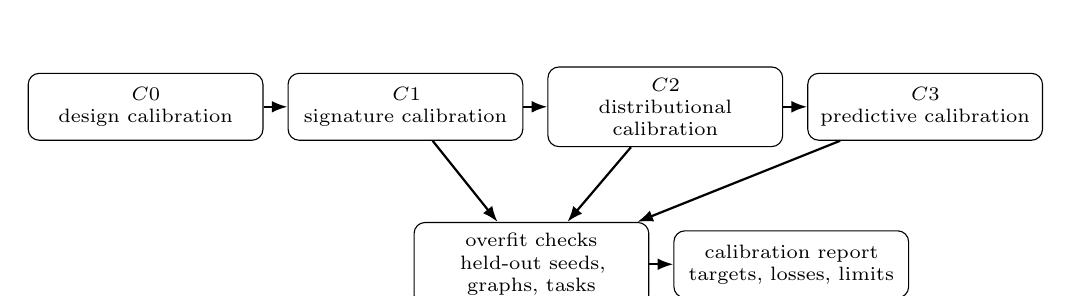
\begin{tikzpicture}[
  x=1cm,y=1cm,
  tier/.style={draw, rounded corners, align=center, text width=2.7cm, minimum height=0.85cm, font=\scriptsize, inner sep=4pt},
  arr/.style={-{Latex[length=2mm]}, thick}
]
\node[tier] (c0) at (0,0) {$C0$\\design calibration};
\node[tier] (c1) at (3.3,0) {$C1$\\signature calibration};
\node[tier] (c2) at (6.6,0) {$C2$\\distributional calibration};
\node[tier] (c3) at (9.9,0) {$C3$\\predictive calibration};
\node[tier] (audit) at (4.9,-2.0) {overfit checks\\held-out seeds, graphs, tasks};
\node[tier] (report) at (8.2,-2.0) {calibration report\\targets, losses, limits};
\draw[arr] (c0) -- (c1); \draw[arr] (c1) -- (c2); \draw[arr] (c2) -- (c3);
\draw[arr] (c1) -- (audit); \draw[arr] (c2) -- (audit); \draw[arr] (c3) -- (audit); \draw[arr] (audit) -- (report);
\end{tikzpicture}%
}
\caption{Calibration governance. Calibration tiers constrain claim strength. Higher tiers require stronger targets and stricter held-out checks; otherwise the simulator may be tuned to produce expected signatures rather than to test mechanisms.}
\label{fig:calibration-governance}
\end{figure}


The simulator is not evidence for the external truth of Dot-Trace Theory by itself. It is a controlled instrument for checking internal coherence, theorem signatures, mechanism interactions, and validation procedures. For that instrument to be useful, its parameters must be governed. A simulator that is tuned after observing the desired result can manufacture apparent support for almost any theory. Calibration must therefore be explicit, limited, reproducible, and separated from validation.

\subsection{Calibration objective}\label{calibration-objective}

Let $\theta$ denote simulator parameters, including memory decay, transmission probability, mutation variance, correction strength, institutional persistence, retrieval sensitivity, access sensitivity, and edge-update sensitivity. Let $s_r^{sim}(\theta)$ be a simulator summary statistic and let $s_r^{target}$ be either a theoretical target, a design target, or a pre-specified empirical proxy. A generic calibration loss is
\[
\mathcal C(\theta)=
\sum_{r=1}^{R}\omega_r\,\Delta_r\big(s_r^{sim}(\theta),s_r^{target}\big)^2
+\lambda_{reg}\|\theta-\theta_0\|^2,
\]
where $\theta_0$ is a documented default configuration. The regularization term is not decorative. It prevents the simulator from drifting into extreme parameter regimes merely to reproduce a target signature.

Calibration targets should be chosen before running validation. Suitable targets include average dot count, access density, retrieval depth, social-edge density, institutional reach, mutation rate, correction latency, fragmentation level, and recursive stability margin. Prediction lift may be used as a validation output, but should not normally be used as the sole calibration target because this risks tuning the simulator to favor the full dot-field model.

\subsection{Calibration tiers}\label{calibration-tiers}

The paper distinguishes four calibration tiers.

\begin{description}[leftmargin=3.2cm,style=nextline]
\item[Tier C0: design calibration]
Parameters are selected to make a mechanism visible. Example: set mutation variance high enough that semantic drift can be measured. C0 is suitable for theorem sanity checks but not for external claims.

\item[Tier C1: signature calibration]
Parameters are selected so that a known theorem signature appears under its assumptions. Example: choose access and edge-update sensitivities so that $\rho(J_\Theta)<1$ produces damping and $\rho(J_\Theta)>1$ produces amplification.

\item[Tier C2: distributional calibration]
Parameters are selected to match observable summaries of a chosen empirical class, such as communication density, archive reach, or correction latency. This tier requires measurement rules and uncertainty intervals.

\item[Tier C3: predictive calibration]
Parameters are selected using training data and evaluated on held-out data under the baseline hierarchy. C3 is the only tier that supports predictive-performance claims.
\end{description}

A simulator run should report its calibration tier. Claims should not exceed the tier. A C0 run can show possibility, not prevalence. A C1 run can check theorem mechanics, not empirical realism. A C2 run can approximate a domain, not prove causality. A C3 run can support held-out prediction claims if leakage controls are passed.

\subsection{Parameter governance table}\label{parameter-governance-table}

Parameter governance records how simulation parameters were chosen, which outputs they influence, and which claims depend on them. This is especially important for dot-field models because several mechanisms can generate similar aggregate patterns. High fragmentation, for example, may result from low bridge probability, strong bonding reinforcement, semantic mutation, access thresholds, or correction failure. Without parameter governance, the same observed signature could be over-interpreted as support for the wrong mechanism.


{\scriptsize
\begin{longtable}{@{}L{0.16\textwidth}L{0.24\textwidth}L{0.21\textwidth}L{0.18\textwidth}@{}}
\caption{Simulator parameters and governance rules.}\label{tab:simulator-parameter-governance}\\
\toprule
\textbf{Parameter class} & \textbf{Examples} & \textbf{Controls} & \textbf{Primary risk}\\
\midrule
\endfirsthead
\toprule
\textbf{Parameter class} & \textbf{Examples} & \textbf{Controls} & \textbf{Primary risk}\\
\midrule
\endhead
Memory lifecycle & $\lambda_m$, reinforcement, forgetting, pruning & Report defaults, sensitivity grid, truncation threshold & Artificial persistence or artificial forgetting\\
Transmission and access & $p_0$, $L_B$, access threshold, bridge floor & Matched seed ablations and access-density targets & Manufacturing spread or closure\\
Retrieval & top-$k$, relevance weights, $L_R$, salience weights & Retrieval recall checks and fixed query rules & Overfitting by selective retrieval\\
Topology feedback & $\eta_w$, $L_E^\zeta$, threshold $\tau$ & Stability-margin and shock tests & Cascades created by parameter choice\\
Mutation and compression & $\epsilon_\mu$, compression frequency, identity threshold & Semantic drift bounds and identity sensitivity & Uncontrolled narrative drift\\
Institutional enc. & $\lambda_I$, archive reach, credibility premium & Institutional reach and persistence audits & Authority bias\\
Correction and repair & counter-dot strength, fit, repair threshold & Correction-latency and residual-harm tests & Unrealistic easy repair or impossible repair\\
Validation & train/test split, negative controls, baseline features & Pre-specified protocol and no-oracle rule & Leakage or unfair baselines\\
\bottomrule
\end{longtable}
}

\subsection{Calibration diagnostics}\label{calibration-diagnostics}

Diagnostics should report both fit and fragility. A low calibration loss is not sufficient if the fit depends on a narrow or unstable parameter setting. The calibration report should therefore include sensitivity to each major mechanism parameter, robustness across random seeds, robustness across graph structures, and performance under withheld signatures. A well-calibrated simulator should reproduce qualitative theorem signatures without requiring a different parameter set for every signature.

The most important diagnostic is the calibration-overfit gap. If the simulator performs well on calibration targets but poorly on held-out conditions, the model may have learned a parameter artifact rather than a robust dot-field mechanism. This problem is especially serious for prediction lift, because highly flexible dot features can memorize generated traces unless temporal splits and negative controls are enforced.


A calibrated run should report at least the following diagnostics:
\[
\mathrm{AD}(t)=\frac{|B_t|}{|A||D_t|}
\]
for access density,
\[
\mathrm{RD}(t)=\frac{1}{|A|}\sum_i |\mathcal V_i(q_i,t)|
\]
for retrieval depth,
\[
\mathrm{MR}(t)=\frac{\text{number of mutated descendant dots at }t}{|D_t|}
\]
for mutation rate,
\[
\mathrm{IR}(t)=\frac{|D_t^I|}{|D_t|}
\]
for institutionalization rate, and
\[
\widehat{SM}(t)=1-\rho(\widehat J_\Theta(t))
\]
for estimated recursive stability margin. A finite-difference estimate of the Jacobian entry is
\[
\widehat J_{ab}=\frac{\Theta_a(e^\star+\delta e_b)-\Theta_a(e^\star)}{\delta},
\]
where $e^\star$ is a reference edge state and $e_b$ is a unit perturbation of the $b$th edge coordinate.

\subsection{Calibration non-identifiability}\label{calibration-non-identifiability}

\begin{proposition}[Simulator calibration non-identifiability]
Suppose a simulator summary $S$ depends on two parameters only through their product, so that
\[
S(\theta_1,\theta_2)=h(\theta_1\theta_2).
\]
Then $\theta_1$ and $\theta_2$ are not separately identifiable from $S$ alone. In particular, for any $c>0$ such that the parameters remain admissible,
\[
h(\theta_1\theta_2)=h((c\theta_1)(\theta_2/c)).
\]
\end{proposition}

\begin{proof}
The equality follows directly from preservation of the product. Since the same observed summary is produced by infinitely many parameter pairs on the curve $\theta_1\theta_2=\mathrm{constant}$, the individual parameters are not separately identified by $S$. Additional summaries, constraints, interventions, or priors are required.
\end{proof}

This simple result matters because many dot-field mechanisms appear only as products in aggregate outputs: access probability times credibility, retrieval sensitivity times salience, correction strength times semantic fit, or edge-update sensitivity times pressure. Calibration reports should therefore state which parameters are independently tuned and which are only jointly constrained.

\subsection{Calibration-report schema}\label{calibration-report-schema}

A calibration report should be treated as part of the scientific output rather than as a supplementary implementation note. It should state the default values, the calibrated values, the target statistics, the calibration loss, the held-out checks, and any parameters that remain weakly identified. When calibration is used only to reproduce qualitative signatures, the report should avoid predictive claims. When predictive calibration is claimed, the report should include temporal separation and negative controls.


Every simulator experiment should include a calibration report with:

\begin{enumerate}[leftmargin=*]
\item simulator version and random seeds;
\item calibration tier C0--C3;
\item parameter table with defaults, calibrated values, and admissible ranges;
\item target statistics and calibration loss;
\item held-out statistics not used for calibration;
\item negative-control results;
\item sensitivity analysis over at least one access, retrieval, topology, and correction parameter;
\item known non-identifiabilities;
\item statement of which claims the calibration tier supports.
\end{enumerate}

The calibration report is part of the scientific artifact. Without it, a simulator output should be treated as an illustration, not as a validation result.

\begin{figure}[htbp]
\centering
\resizebox{0.94\textwidth}{!}{%
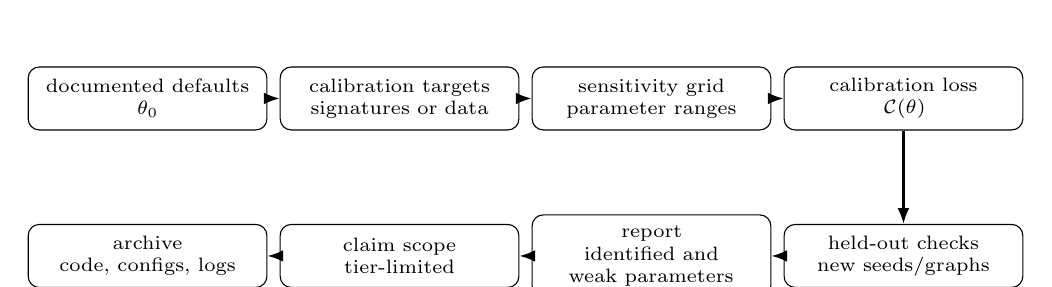
\begin{tikzpicture}[
  x=1cm,y=1cm,
  box/.style={draw, rounded corners, align=center, text width=2.75cm, minimum height=0.8cm, font=\scriptsize, inner sep=4pt},
  arr/.style={-{Latex[length=2mm]}, thick}
]
\node[box] (defaults) at (0,0) {documented defaults\\$\theta_0$};
\node[box] (targets) at (3.2,0) {calibration targets\\signatures or data};
\node[box] (grid) at (6.4,0) {sensitivity grid\\parameter ranges};
\node[box] (fit) at (9.6,0) {calibration loss\\$\mathcal C(\theta)$};
\node[box] (holdout) at (9.6,-2.0) {held-out checks\\new seeds/graphs};
\node[box] (report) at (6.4,-2.0) {report\\identified and weak parameters};
\node[box] (claims) at (3.2,-2.0) {claim scope\\tier-limited};
\node[box] (archive) at (0,-2.0) {archive\\code, configs, logs};
\draw[arr] (defaults) -- (targets); \draw[arr] (targets) -- (grid); \draw[arr] (grid) -- (fit); \draw[arr] (fit) -- (holdout);
\draw[arr] (holdout) -- (report); \draw[arr] (report) -- (claims); \draw[arr] (claims) -- (archive);
\end{tikzpicture}%
}
\caption{Simulator calibration workflow. A calibration report should preserve default parameters, calibration targets, search ranges, objective values, held-out performance, and the resulting claim scope.}
\label{fig:calibration-workflow}
\end{figure}



\section{Falsifiability and Failure Modes}\label{falsifiability-failure-modes}

A theory of trace-mediated social systems must specify how it can fail. Dot-Trace Theory is not supported merely by finding messages, memories, records, or archives in a social setting; many social systems contain such material. The theory earns explanatory value only when explicit dot-field variables improve representation, explanation, prediction, correction, or intervention relative to appropriate reduced models. Failure is therefore informative: it identifies where the ontology is unnecessary, where measurement is too weak, where a proposed mechanism is inactive, where prediction does not improve, or where causal claims are unsupported.

\begin{longtable}{L{0.20\linewidth}L{0.34\linewidth}L{0.34\linewidth}}
\caption{Failure modes for Dot-Trace Theory.}\label{tab:failure-modes}\\
\toprule
\textbf{Failure type} & \textbf{Meaning} & \textbf{Diagnostic signature}\\
\midrule
\endfirsthead
\toprule
\textbf{Failure type} & \textbf{Meaning} & \textbf{Diagnostic signature}\\
\midrule
\endhead
Representational & Dot variables add no transition-relevant information beyond $Z_t$. & Conditional mutual information or held-out prediction lift is approximately zero under adequate measurement.\\
Measurement & Dots, access, provenance, credibility, or retrieval cannot be observed, inferred, or bounded with sufficient reliability. & Low extraction reliability, high access uncertainty, unstable canonicalization, or outcome-aware coding.\\
Mechanism & A proposed dot mechanism is inactive in the target system. & Ablating the mechanism does not change trajectories, predictions, or relevant process signatures.\\
Predictive & Dot-field features do not outperform strong reduced baselines. & Held-out loss is not lower than temporal edge, flat-memory, or bag-of-dots alternatives.\\
Causal & Dot variables predict outcomes but interventions on access, retrieval, correction, or institutionalization do not change outcomes as predicted. & Randomized exposure, natural experiments, instruments, or structural interventions fail to produce the expected effect.\\
Governance & A formally valid dot-field model creates unacceptable privacy, reputational, or institutional risk. & The model lacks contestability, access minimization, retention limits, or auditability for consequential traces.\\
\bottomrule
\end{longtable}

\subsection{Representational failure}\label{representational-failure}

Representational failure is the strongest objection to applying the theory in a particular domain. It occurs when the reduced state $Z_t$ already carries all transition-relevant information. Formally, if
\[
I(Y_{t+1};D_t,R_t^D,B_t,\mathbf M_t,Q_t,L_t\mid Z_t)=0,
\]
then explicit dot-field variables add no predictive information for the specified outcome and horizon. This does not imply that traces do not exist. It implies that, for the model and task under study, they do not need to be represented separately.

A serious application should therefore compare the dot-field model against strong reduced baselines, not only against weak edge-only models. If a temporal edge model with adequate history features matches the dot-field model under held-out evaluation and negative controls, the appropriate conclusion is domain-specific: the reduced representation may already encode a dot-sufficient statistic. Dot-Trace Theory is a conditional representational theory, and representational failure is one of its legitimate boundary outcomes.

\subsection{Measurement failure}\label{measurement-failure}

Measurement failure occurs when theoretical objects cannot be recovered with enough reliability for the proposed claim. A dataset may contain messages but not provenance, records but not access, access logs but not attention, attention but not retrieval, or retrieval traces but not belief. Each missing layer restricts what can be asserted. The measurement protocol therefore requires observability grades, explicit uncertainty, and measurement-admissibility rules.

The most common risks are access inflation and semantic misclassification. Access inflation treats every public trace as if every agent encountered it. Semantic over-merging treats distinct lineages as the same dot because their surface wording is similar; semantic over-splitting treats equivalent traces as unrelated because they differ in form. These errors can change estimates of convergence, correction reach, social capital, and fragmentation. Measurement failure is therefore not merely statistical noise; it can reverse the substantive interpretation of the dot field.

\subsection{Mechanism failure}\label{mechanism-failure}

Mechanism failure occurs when dots exist but the proposed dot process is not operative. A system may store institutional records that agents never retrieve; a correction may be publicly available but never reach the affected component; evaluative dots may exist while social edges update through exogenous incentives; or traces may transmit without mutation in a setting where semantic drift was hypothesized.

Mechanism failure should be evaluated by ablation, process logs, and intervention where feasible. Removing mutation should reduce drift only if mutation is active. Removing topology feedback should alter edge trajectories only if trace-mediated edge update is operative. This is why the theory separates representation from mechanism: the existence of a dot field does not imply that every dot mechanism is active in every domain.

\subsection{Predictive failure}\label{predictive-failure}

Predictive failure occurs when dot-field features do not improve held-out prediction relative to appropriate alternatives. Such failure can have several interpretations. The theory may be unnecessary for the target outcome; the measurement window may be too short; the extracted dots may be poor proxies; the reduced baseline may already contain a sufficient statistic; or the domain may be driven by exogenous shocks rather than trace-mediated action.

A credible predictive test must therefore include temporal separation, strong baselines, uncertainty estimates, and negative controls. A model that performs well only because future traces leak into training features, because labels are encoded in extracted dots, or because target identities are not properly separated has not demonstrated dot-field value. Prediction lift is evidence only when it survives controls that would destroy spurious trace alignment.

\subsection{Causal failure}\label{causal-failure}

Causal failure occurs when dot-field variables predict outcomes but interventions on those variables do not change outcomes. A negative evaluative dot may correlate with distrust because both are caused by an unobserved conflict. A high-centrality institutional dot may predict coordination because it is created after successful coordination has already occurred. In such cases, dots may be valid descriptors or predictors without being the causal mechanism.

Causal claims require stronger designs: randomized exposure, natural experiments, instrumental variation, longitudinal interventions, or explicit structural assumptions. Dot-Trace Theory can be used descriptively, predictively, or causally, but these uses require different evidence. The presence of a trace does not by itself show that the trace caused later action.

\subsection{Governance failure}\label{governance-failure}

A dot-field account can also fail ethically even when it succeeds formally. A system may improve prediction by retaining sensitive traces, surfacing reputational labels without contestability, amplifying old accusations, or making inferred dots available to agents who should not have access to them. In high-stakes settings, such a system is not ready for deployment merely because its transition model is accurate.

Governance failure is therefore a substantive failure mode. Applications should specify access minimization, retention policy, correction rights, auditability, uncertainty labeling, and procedures for repair. The same representation that makes social memory visible can also make surveillance and manipulation easier. Scientific usefulness and responsible use must be evaluated together.

\section{Measurement and Dot-Extraction Protocol}\label{measurement-dot-extraction-protocol}

Dot-Trace Theory requires an operational bridge between the formal object
\(d\in D_t\) and observable material such as messages, records, actions,
issues, tickets, conversation turns, memories, annotations, archives, or
agent logs. Without such a bridge, the theory risks becoming a vocabulary
for retrospective interpretation rather than a measurable framework. This
section therefore specifies a measurement protocol: what counts as a dot,
what should be excluded, how dot identity is handled, how provenance and
access are coded, how measurement uncertainty is represented, and how
extraction quality should be audited before empirical claims are made.

The protocol is intentionally conservative. It does not require every
human memory or latent belief to be directly observed. It requires that an
empirical study distinguish observed dots, inferred dots, latent dots, and
inadmissible pseudo-dots. A dot-field analysis is only as strong as the
observability and coding discipline behind \(D_t\), \(R_t^D\), \(B_t\),
\(\mathbf M_t\), \(Q_t\), and \(L_t\).

\subsection{Measurement stance}\label{measurement-stance}

The measurement stance of Dot-Trace Theory is conservative. The theory does not assume that all relevant dots are directly observable, nor does it treat every utterance as a dot. A trace becomes a measured dot only when its content, persistence, provenance, access route, and action relevance can be coded with explicit uncertainty. This prevents the framework from inflating unstructured text into an all-purpose explanatory device.


The theory distinguishes three levels of measurement.

\begin{description}[leftmargin=3.2cm,style=nextline]
\item[Observed dots]
Traces directly present in the data: a message, event log, institutional
record, ticket, post, archive entry, annotation, retrieval log, or
explicit memory entry.

\item[Inferred dots]
Traces not directly observed but inferable from structured evidence, such
as repeated references to an earlier claim, a visible reply to an unseen
message, or an edge update that can be linked to a known testimonial.

\item[Latent dots]
Traces that may exist inside an agent but are not directly observed and
cannot be uniquely inferred from available data. Latent dots may be
modeled statistically, but claims about them require weaker language.
\end{description}

Empirical applications using Dot-Trace Theory state which measurement level they use. The strongest measurement claims concern observed dots. The weakest
concern latent dots inferred only from behavior.

\subsection{Unit of observation}\label{unit-of-observation}

The unit of observation depends on the empirical setting. In a collaborative software system, it may be a message, ticket, commit, postmortem, or access-log event. In an organizational study, it may be an incident report, meeting minute, policy document, or recorded decision. In an agent simulation, it may be a generated memory item, tool output, or public artifact. The coding protocol must specify the record type before dot extraction begins, because different record types support different claims about provenance, access, attention, and retrieval.


Let \(y_r\) denote an observed trace-bearing unit in a dataset. Depending
on the domain, \(y_r\) may be a sentence, message, meeting note, issue
comment, pull request, transaction record, moderation decision, memory
retrieval event, social-media post, fact-check, institutional policy, or
agent-generated reflection. The extraction function maps observable units
to candidate dots:
\[
\mathcal E:Y\rightarrow \mathcal P(D),
\]
where \(\mathcal P(D)\) is the finite set of dots extracted from the
observed unit. A single observation may create no dot, one dot, or
multiple dots. For example, a message may contain a promise, an evaluation
of an agent, and a correction of a prior claim; these should be separable
when they have different targets, provenance, valence, or future action
relevance.

\subsection{Minimum dot test}\label{minimum-dot-test}

A candidate trace is coded as a dot only if it passes the minimum
dot test.

\begin{definition}[Minimum dot test]
An observed or inferred trace \(y_r\) is admissible as a dot candidate if
it satisfies five conditions:
\begin{enumerate}[leftmargin=*]
\item \textbf{Content:} it encodes a claim, event, observation,
evaluation, rule, obligation, record, correction, summary, or
interpretation.
\item \textbf{Persistence:} it can remain available beyond the moment of
creation, either in memory, conversation, artifact, archive, log, or
institutional record.
\item \textbf{Provenance:} its source, creator, witness, transmitter, or
institutional location can be assigned, observed, or estimated.
\item \textbf{Access:} at least one agent has a plausible route to
retrieve, observe, receive, cite, or act upon it.
\item \textbf{Action relevance:} it can plausibly affect belief, choice,
trust, coordination, reputation, correction, social capital, or topology.
\end{enumerate}
\end{definition}

A candidate that fails one or more conditions may still be useful as raw
data, but it should not be treated as a dot without qualification. The
minimum dot test is deliberately stricter than ordinary text extraction:
not every sentence is a dot, and not every logged event is a dot.

\subsection{Exclusion and boundary rules}\label{exclusion-boundary-rules}

The following cases should be excluded or flagged.

\begin{description}[leftmargin=3.2cm,style=nextline]
\item[Transient stimulus]
A momentary stimulus with no persistence, storage, citation, or
retrievability is not a dot for the purposes of this theory.

\item[Pure social edge]
The existence of a tie \((a_i,a_j)\) is not itself a dot. A dot may explain
why the tie exists, changes, strengthens, or weakens, but the edge and the
trace should remain distinct.

\item[Outcome-only pseudo-dot]
An analyst should not create a dot merely because an outcome occurred. For
example, if trust decreased, the decrease itself is not evidence of a
specific negative dot unless a trace or trace proxy is observed or
identified by a justified model.

\item[Unassigned aggregate attribute]
A broad label such as ``team culture'' or ``low morale'' is not a dot
unless it is linked to specific trace content, source, access, and
persistence.

\item[Duplicate surface form]
Repeated copies of the same content should not automatically be coded as
independent dots. They may be separate tokens, but they may also belong to
the same lineage or semantic identity class.

\item[Inaccessible artifact]
A record that exists but is inaccessible to all modeled agents during the
relevant time window should not be included in \(B_t\) as an actionable
dot, although it may be retained as an external archive.
\end{description}

Boundary cases should be recorded rather than hidden. A useful protocol
should distinguish ``not a dot,'' ``dot candidate,'' ``observed dot,''
``inferred dot,'' and ``latent dot.''

\subsection{Coding workflow}\label{coding-workflow}

A reproducible dot-extraction workflow proceeds in stages.

\begin{enumerate}[leftmargin=*]
\item \textbf{Segment the record:} define the atomic observation units
\(y_r\), such as messages, turns, comments, records, or sentences.
\item \textbf{Apply the minimum dot test:} decide whether each unit
contains zero, one, or multiple candidate dots.
\item \textbf{Assign dot type:} classify each dot as observational,
interactional, testimonial, evaluative, normative, reflective, mutated,
compressed, institutional, counter-dot, repair dot, or other specified
type.
\item \textbf{Extract content and target:} record the semantic content
\(x(d)\) and, where relevant, the target agent, object, group, rule,
claim, or prior dot.
\item \textbf{Code provenance:} record creator, transmitter, witness,
archive, source document, channel, and timestamp.
\item \textbf{Code access:} determine which agents could access the dot
and whether access is observed, inferred, or unknown.
\item \textbf{Code relations:} add support, contradiction, citation,
summary, mutation, lineage, target, institutionalization, and correction
relations.
\item \textbf{Estimate strengths:} assign or estimate salience,
credibility, affective charge, normative force, memory weight, and
effective retrievable strength when data support such estimates.
\item \textbf{Audit and adjudicate:} compare coders or algorithms,
resolve disagreements, and record uncertainty.
\item \textbf{Freeze the extraction rule:} do not revise extraction rules
after seeing outcome-model results unless the revision is reported as
exploratory.
\end{enumerate}

The last step is important. Otherwise, dots can be overfit to explain the
outcome after the fact.

\begin{algorithmblock}{Dot extraction and measurement workflow}
\label{alg:dot-extraction-workflow}
\item \textbf{Input:} raw records such as messages, transcripts, tickets, logs, archives, institutional entries, or instrumented agent traces.
\item \textbf{Output:} coded dot dataset with identifiers, attributes, provenance, access estimates, relation labels, uncertainty grades, and audit records.
\item Segment the data into observation units such as messages, turns, records, tickets, logs, or institutional entries.
\item Apply the minimum dot test: content, persistence, provenance, access, and plausible action relevance.
\item Assign dot type, target, context, timestamp, provenance, access grade, and uncertainty grade.
\item Canonicalize duplicate or semantically equivalent candidates while preserving token, lineage, and semantic identity distinctions.
\item Code dot-dot relations, including support, contradiction, citation, summary, mutation, lineage, target, institutionalization, and correction.
\item Estimate salience, credibility, valence, normative force, memory weight, and effective strength only when the observability grade supports the estimate.
\item Audit the extraction through coder agreement, negative controls, outcome-blind coding, and sensitivity analysis.
\item Freeze the extraction rule before confirmatory outcome modeling.
\end{algorithmblock}


\subsection{Dot identity and canonicalization}\label{dot-identity-canonicalization-protocol}

Dot identity is not a single relation. The protocol should track at least
three identity levels.

\begin{description}[leftmargin=3.2cm,style=nextline]
\item[Token identity]
Two dots are token-identical only if they are the same observed trace
instance with the same identifier.

\item[Lineage identity]
Two dots share lineage identity if one descends from the other through
quotation, transmission, paraphrase, mutation, summarization,
institutional rewriting, or correction history. Formally, this is
reachability in the lineage graph \(L_t\).

\item[Semantic identity]
Two dots are semantically equivalent for task \(\tau\) when their semantic
distance is below a task-specific threshold:
\[
\Delta_{\mathcal X}(x(d),x(e))\leq \theta_\tau.
\]
\end{description}

The task dependence matters. Two paraphrases may be equivalent for
predicting broad cooperation but not equivalent for legal attribution,
credit assignment, or correction of a precise false claim.

Canonicalization should therefore retain the raw token, the lineage link,
and the semantic cluster. A recommended canonical dot record stores
\[
(id_{token},id_{lineage},id_{semantic,\tau}).
\]
This prevents a common measurement error: collapsing distinct trace tokens
into a single abstract statement and thereby losing timing, provenance,
and access information.

\subsection{Attribute schema}\label{attribute-schema}

The attribute schema is designed to prevent dots from becoming vague labels. At minimum, a coded dot should include content, time, provenance, target, type, access status, lifecycle state, and uncertainty. Stronger datasets may add salience, credibility, valence, semantic embedding, institutional anchor, lineage, and relation edges. The schema should be applied consistently across positive, negative, neutral, and corrective traces so that the model does not privilege reputationally salient dots while ignoring mundane but behaviorally important traces.


Every coded dot should include a minimal attribute schema. The schema can
be expanded for specific domains, but the following fields are the
recommended core.

{\small
\begin{longtable}{L{0.22\textwidth}L{0.34\textwidth}L{0.34\textwidth}}
\caption{Recommended dot attribute schema.}\label{tab:dot-attribute-schema}\\
\toprule
\textbf{Field} & \textbf{Meaning} & \textbf{Examples or admissible values}\\
\midrule
\endfirsthead
\toprule
\textbf{Field} & \textbf{Meaning} & \textbf{Examples or admissible values}\\
\midrule
\endhead
\bottomrule
\endlastfoot
Dot identifier & Unique token id. & \(d_{103}\), message-turn id, issue-comment id.\\
Content \(x(d)\) & Semantic content. & Claim, event, promise, accusation, correction, summary.\\
Type & Dot class. & Observational, testimonial, evaluative, normative, institutional, counter-dot.\\
Creation time \(\tau(d)\) & Time or sequence position. & Timestamp, round number, message order.\\
Provenance \(p(d)\) & Source, creator, witness, transmitter, archive. & Author, channel, cited document, system log.\\
Target \(T(d)\) & Entity, claim, agent, or rule the dot concerns. & Agent, team, document, prior dot, norm.\\
Context \(c(d)\) & Situation of creation. & Meeting, thread, task, crisis, experiment round.\\
Access set \(B_{\cdot d}(t)\) & Agents who could access the dot. & Readers, subscribers, channel members, retrieval recipients.\\
Access grade & Strength of access evidence. & Observed, inferred, possible, unknown.\\
Salience \(\sigma(d)\) & Likelihood of attention or retrieval. & Repetition, rank, prominence, emotional intensity.\\
Credibility \(\gamma_i(d,t)\) & Agent-relative trust in the dot. & Source trust, verification, institutional status.\\
Valence \(v_i(d,t)\) & Evaluative direction for a target. & Positive, negative, neutral, mixed; scalar in \([-1,1]\).\\
Normative force & Whether it imposes a rule, duty, taboo, or expectation. & Obligation, permission, prohibition, standard.\\
Lifecycle state \(\ell(d,t)\) & Current status of the dot. & Active, decayed, corrected, archived, deleted, contested.\\
Relations \(R_t^D\) & Dot-dot links. & Supports, contradicts, cites, summarizes, mutates, repairs.\\
Lineage \(L_t\) & Ancestors and descendants. & Parent quote, paraphrase, translation, compressed summary.\\
Institutional anchor & Whether the dot is stored in a durable institution. & Policy, contract, database, archive, ledger, ticket.\\
Uncertainty & Confidence in coding. & Coder confidence, model probability, adjudication flag.\\
\end{longtable}
}

The schema does not require every field to be fully observed. It requires
that missingness be explicit. Unknown provenance, unobserved access, or
uncertain valence should be coded as uncertainty, not silently filled.

\subsection{Access, attention, and retrieval}\label{access-attention-retrieval-measurement}

Dot access should not be confused with attention or retrieval. The access
relation \(B_t\) records whether an agent could access a dot. Attention
records whether the agent likely noticed it. Retrieval records whether the
agent later used it in a decision context.

A measurement protocol should therefore distinguish:
\[
\widehat B_{id}(t)=P((a_i,d)\in B_t\mid Y_{0:t}),
\]
\[
\widehat A_{id}(t)=P(a_i\text{ attended to }d\mid Y_{0:t}),
\]
and
\[
\widehat R_{id}(q,t)=P(d\in \mathcal V_i(q,t)\mid Y_{0:t}).
\]

Access can be observed through read receipts, subscriptions, channel
membership, permissions, citations, downloads, retrieval logs, or direct
experimental exposure. Attention may require dwell time, response
content, recall, ranking position, or self-report. Retrieval is strongest
when the agent explicitly cites the dot, repeats it, acts in ways tied to
it under a specified model, or when a system log records memory retrieval.

A common measurement error is to infer retrieval from access alone. The
protocol should instead represent access as a necessary but not sufficient
condition for retrieval.

\subsection{Provenance and credibility}\label{provenance-credibility-measurement}

Provenance is the history of how a dot came to be present in the dot
field. Credibility is the agent-relative weight given to that dot.
Provenance can often be coded more directly than credibility. A message
author or archive location may be observed, while credibility may have to
be inferred from prior trust, verification status, institutional role,
endorsement, contradiction, or subsequent use.

A useful decomposition is
\[
\gamma_i(d,t)=g_i(Source(d),Evidence(d),Institution(d),History_i(d),Context(d)).
\]
This expression is not a universal model; it is a reminder that
credibility is agent-relative and context-dependent. A dot from the same
source may be credible in one domain and not another.

Provenance coding should include at least:
\begin{enumerate}[leftmargin=*]
\item original creator or first observed source;
\item transmitter or mediator, if different from creator;
\item channel or archive;
\item timestamp or order position;
\item version or mutation parent;
\item institutional status, if any;
\item uncertainty or missingness code.
\end{enumerate}

\subsection{Dot relations}\label{dot-relation-measurement}

Dot relations determine whether the dot field is merely a collection of traces or a structured memory system. Relations may encode support, contradiction, temporal precedence, causal attribution, semantic similarity, lineage, compression, repair, or institutional anchoring. The relation vocabulary should be small enough to code reliably but expressive enough to represent the mechanisms being tested. For example, a study of correction must code contradiction and target-fit relations, while a study of mutation must code lineage and semantic drift.


The dot graph \(G_t^D=(D_t,R_t^D)\) should be coded with typed relations.
At minimum, the following relation types are recommended:

\begin{longtable}{L{0.22\textwidth}L{0.34\textwidth}L{0.34\textwidth}}
\toprule
\textbf{Relation} & \textbf{Meaning} & \textbf{Example}\\
\midrule
\endhead
Supports & One dot increases support for another. & A witness statement supports a claim.\\
Contradicts & One dot challenges another. & A correction contradicts a rumor.\\
Cites & One dot explicitly refers to another source. & A report cites an earlier document.\\
Summarizes & One dot compresses a set of dots. & Meeting minutes summarize discussion.\\
Mutates & One dot descends with changed meaning. & A rumor becomes exaggerated.\\
Targets & A dot evaluates or concerns an agent or object. & ``Agent B missed the deadline.''\\
Institutionalizes & A dot is encoded into a durable artifact. & A policy records a norm.\\
Repairs & A dot attempts social repair after harm. & Apology, retraction, compensation.\\
\bottomrule
\end{longtable}

Relation coding should be directional when direction matters. For example,
\(c\dashv d\) means that counter-dot \(c\) challenges target dot \(d\),
not necessarily the reverse. Relation confidence should be stored as
\[
\widehat r_{de}^{type}(t)\in[0,1].
\]

\subsection{Valence, targets, and normative force}\label{valence-targets-norms-measurement}

Valence should be coded relative to a target and a decision context. The same trace may be positive for one agent, negative for another, and normatively ambiguous for a third. For example, a whistleblowing dot may damage the reputation of one actor while increasing the credibility of another and strengthening an institutional norm. Coding should therefore separate target, evaluator, and normative frame. Normative force should be reserved for traces that express obligations, prohibitions, permissions, sanctions, or role expectations rather than for all emotionally charged traces.


Evaluative and normative dots require special care because they directly
affect topology, reputation, exclusion, and social capital. A dot's
valence should be coded relative to a target and an interpreting agent:
\[
\widehat v_i(d,j,t)\in[-1,1].
\]
The same trace may be positive for one agent and negative for another. A
managerial warning may be interpreted as helpful by one agent and hostile
by another. A norm may benefit insiders and constrain outsiders.

The protocol should therefore distinguish target identity, valence,
normative mode, evaluator perspective, and confidence.

\subsection{Memory weight and effective strength}\label{memory-weight-effective-strength-measurement}

The formal theory uses memory weight \(m_i(d,t)\) and effective
retrievable strength \(Q_i(d,t)\). In empirical work these quantities are
usually estimated, not directly observed. A practical measurement model is
\[
\widehat Q_i(d,t)=\widehat b_i(d,t)\widehat\gamma_i(d,t)\widehat m_i(d,t),
\]
where \(\widehat b_i(d,t)\) estimates access, \(\widehat\gamma_i(d,t)\)
estimates credibility, and \(\widehat m_i(d,t)\) estimates memory weight
or retrieval salience.

Candidate proxies include access logs, read receipts, channel membership,
retrieval count, recency, repetition, dwell time, recall, ranking
position, source trust, verification, institutional role, cross-source
agreement, emotional intensity, explicit tagging, archival status, and
correction status. The protocol should report which proxy is used and
which component of \(Q_i\) it approximates. A single proxy should not be
allowed to stand for access, credibility, and memory weight
simultaneously unless the study explicitly treats \(Q_i\) as an aggregate
latent score.

\subsection{Reliability and auditability}\label{reliability-auditability-measurement}

Reliability has at least two forms. Coding reliability concerns whether different coders or extraction models identify the same dots, attributes, and relations. Process auditability concerns whether the dataset preserves enough provenance to reconstruct why a dot was coded in a particular way. A dot-field study should report both. High agreement on low-provenance codes is not enough, because later researchers must also be able to inspect the evidence behind consequential trace claims.


Extraction reliability should be measured at several levels: dot
detection reliability, boundary reliability, attribute reliability,
relation reliability, and outcome blindness. For binary dot detection, a
simple extraction F1 score can be used when a reference coding exists:
\[
F1_D=\frac{2TP_D}{2TP_D+FP_D+FN_D}.
\]
For relation extraction, the analogous score is
\[
F1_R=\frac{2TP_R}{2TP_R+FP_R+FN_R}.
\]
For continuous attributes such as valence or credibility, report mean
absolute disagreement or intraclass correlation where appropriate:
\[
MAD_v=\frac{1}{N}\sum_{r=1}^N|\widehat v_r^{(1)}-\widehat v_r^{(2)}|.
\]

Auditability requires that every coded dot can be traced back to raw data,
a coding decision, a coder or algorithm version, and a timestamp. The
recommended audit tuple is
\[
(id_d,id_{raw},coder,ruleversion,time,decision,confidence).
\]

\subsection{Observability ladder for measurement}\label{observability-ladder-measurement}

The observability ladder links data quality to claim strength. Action-only data can sometimes identify aggregate pressure, but they cannot identify dot composition. Communication data can reveal trace tokens, but not necessarily attention or retrieval. Access logs improve exposure measurement, retrieval logs improve behavioral interpretation, and randomized exposure or instrumented memory provides the strongest causal leverage. A claim should not be stated at a higher observability level than the data support.


Dot-field studies should grade observability before making strong claims.

{\small
\begin{longtable}{L{0.12\textwidth}L{0.36\textwidth}L{0.40\textwidth}}
\caption{Observability grades for dot-field measurement.}\label{tab:measurement-observability-ladder}\\
\toprule
\textbf{Grade} & \textbf{Available evidence} & \textbf{Permitted claim strength}\\
\midrule
\endfirsthead
\toprule
\textbf{Grade} & \textbf{Available evidence} & \textbf{Permitted claim strength}\\
\midrule
\endhead
\bottomrule
\endlastfoot
O0 & No trace records; actions only. & Do not claim dot composition; at most infer aggregate pressure.\\
O1 & Trace content observed but provenance or access missing. & Descriptive dot catalog; weak causal or access claims.\\
O2 & Content and provenance observed; access partially inferred. & Moderate claims about source and trace structure; cautious access claims.\\
O3 & Content, provenance, and access logs observed. & Stronger dot-field reconstruction and predictive validation.\\
O4 & Retrieval, attention, or citation logs observed. & Stronger memory-action and retrieval claims.\\
O5 & Randomized exposure or instrumented agent memory. & Strongest causal claims about dot exposure and retrieval.\\
\end{longtable}
}

A study at O1 should not make claims that require O4. This is a central
measurement-discipline rule for the theory.

\subsection{Measurement admissibility}\label{measurement-admissibility}

\begin{definition}[Measurement-admissible dot dataset]
A coded dataset \(\widehat\Omega_{0:T}\) is measurement-admissible for a
specified claim \(\mathcal C\) if it satisfies four conditions:
\begin{enumerate}[leftmargin=*]
\item the dot extraction rule is stated before the main outcome analysis;
\item each theoretical object used in \(\mathcal C\) has an observed,
inferred, latent, or unavailable measurement status;
\item extraction uncertainty is recorded for dots, access, relations, and
attributes used by the claim;
\item the claim strength does not exceed the dataset's observability grade.
\end{enumerate}
\end{definition}

This definition does not guarantee correctness. It guarantees that the
measurement basis of the claim is explicit enough to be audited.

\begin{proposition}[Prediction stability under bounded extraction error]
Suppose a dot-field predictor maps an extracted feature vector
\(F_i(t)\) to an action probability \(p_i(t)=\pi(F_i(t))\), where
\(\pi\) is \(L_\pi\)-Lipschitz. Let \(\widehat F_i(t)\) be the measured
feature vector and assume
\[
\|\widehat F_i(t)-F_i(t)\|\leq \varepsilon.
\]
Then
\[
|\pi(\widehat F_i(t))-\pi(F_i(t))|\leq L_\pi\varepsilon.
\]
If probabilities are clipped to \([\alpha,1-\alpha]\) with
\(0<\alpha<1/2\), then the absolute difference in binary log loss for a
single observation is bounded by
\[
|\ell_{LL}(y,\pi(\widehat F_i(t)))-\ell_{LL}(y,\pi(F_i(t)))|
\leq \frac{L_\pi}{\alpha(1-\alpha)}\varepsilon.
\]
\end{proposition}

\begin{proof}
The first inequality follows directly from Lipschitz continuity. For the
second, the derivative of binary log loss with respect to predicted
probability is \(-y/p+(1-y)/(1-p)\). On \([\alpha,1-\alpha]\), its
absolute value is bounded by \(1/(\alpha(1-\alpha))\). The result follows
from the mean-value theorem and the first inequality.
\end{proof}

\subsection{Measurement threats}\label{measurement-threats}

Measurement threats should be reported as part of the study design rather than discovered after modeling. Over-extraction increases the apparent density of the dot field and can make meaningless traces look causal. Under-extraction removes counter-dots, corrections, and weak ties, often exaggerating fragmentation. Provenance loss makes credibility and source effects impossible to evaluate. Access inflation turns public availability into assumed exposure. Semantic over-merging erases contested meaning; semantic over-splitting prevents convergence from being detected. Outcome-aware coding is especially dangerous because it can turn later behavior into an artificial explanation for itself.

The practical response is to separate coding from outcome modeling when possible, document uncertainty, report inter-coder reliability or model confidence, and run sensitivity analyses. A dot-field study should be able to state how its conclusions change when ambiguous dots are removed, when access is treated conservatively, and when semantic identity thresholds vary.


The main threats to dot measurement are over-extraction, under-extraction,
outcome leakage, access inflation, provenance loss, semantic over-merging,
semantic over-splitting, valence ambiguity, institutional authority bias,
and unmeasured counter-dots. A credible empirical study should report
which threats are most relevant and how they were mitigated.


\begin{figure}[htbp]
\centering
\resizebox{0.98\textwidth}{!}{%
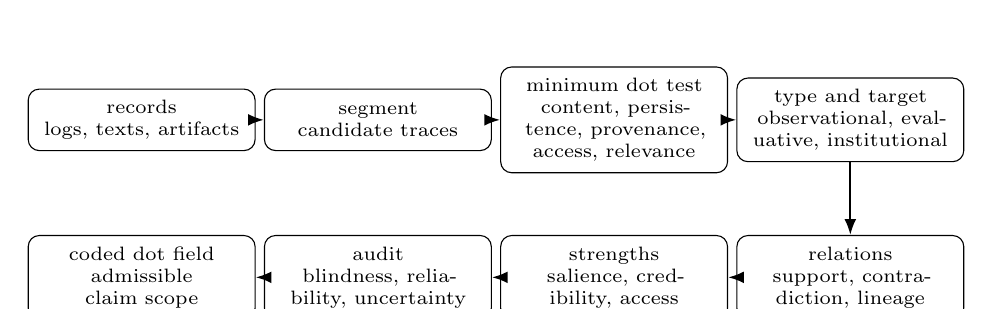
\begin{tikzpicture}[
  x=1cm,y=1cm,
  box/.style={draw, rounded corners, align=center, text width=2.6cm, minimum height=0.78cm, font=\scriptsize, inner sep=4pt},
  arr/.style={-{Latex[length=2mm]}, thick}
]
\node[box] (record) at (0,0) {records\\logs, texts, artifacts};
\node[box] (segment) at (3,0) {segment\\candidate traces};
\node[box] (test) at (6,0) {minimum dot test\\content, persistence, provenance, access, relevance};
\node[box] (type) at (9,0) {type and target\\observational, evaluative, institutional};
\node[box] (relations) at (9,-2) {relations\\support, contradiction, lineage};
\node[box] (strengths) at (6,-2) {strengths\\salience, credibility, access};
\node[box] (audit) at (3,-2) {audit\\blindness, reliability, uncertainty};
\node[box] (dataset) at (0,-2) {coded dot field\\admissible claim scope};
\draw[arr] (record) -- (segment); \draw[arr] (segment) -- (test); \draw[arr] (test) -- (type); \draw[arr] (type) -- (relations);
\draw[arr] (relations) -- (strengths); \draw[arr] (strengths) -- (audit); \draw[arr] (audit) -- (dataset);
\end{tikzpicture}%
}
\caption{Dot-extraction workflow. The protocol separates record segmentation from the decision that a trace is a dot. It then codes type, target, provenance, access, relations, strength, and uncertainty before assigning claim scope.}
\label{fig:dot-extraction-workflow}
\end{figure}


\subsection{Measurement protocol outputs}\label{measurement-protocol-outputs}

The output of the protocol should be a structured dot dataset, not only a narrative codebook. At minimum, the dataset should contain dot identifiers, content representation, provenance, time, target, type, access set, retrieval evidence if available, credibility estimate, salience estimate, valence, relations, lineage, lifecycle state, and uncertainty. It should also specify which fields are observed, inferred, or latent.

A second output is an observability report. This report states the observability grade, extraction reliability, access uncertainty, relation reconstruction quality, and known blind spots. A third output is a modeling interface that maps coded dots into the formal objects $D_t$, $R_t^D$, $B_t$, $\mathbf M_t$, $Q_t$, and $L_t$. Without this mapping, the measurement protocol does not actually connect to the theory.


A complete measurement protocol includes a domain-specific codebook,
positive and negative examples, a dot attribute template, an access and
retrieval measurement plan, a provenance and lineage schema, relation
coding rules, an observability-grade assessment, a reliability report, a
measurement-error sensitivity analysis, and a prespecified rule for
freezing or revising the extraction protocol. These outputs make dot-field
measurement auditable and reduce the risk that dots are defined
retroactively to fit observed outcomes.

\section{Experimental Validation and Benchmarking Protocol}\label{experimental-validation-and-benchmarking-protocol}

Figure~\ref{fig:validation-stack} summarizes the benchmarking logic. The goal is not to show that the full model always wins. The goal is to identify the conditions under which each additional dot-field layer contributes measurable value, and to verify that this value disappears or weakens under appropriate negative controls.

\begin{figure}[htbp]
\centering
\resizebox{0.96\textwidth}{!}{%
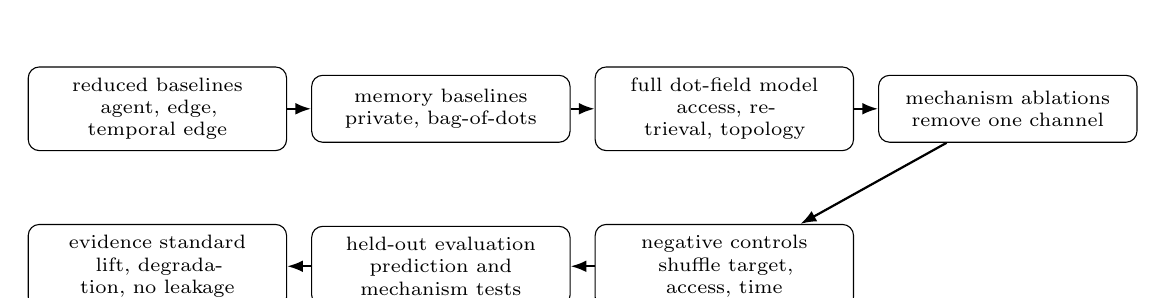
\begin{tikzpicture}[
  x=1cm,y=1cm,
  box/.style={draw, rounded corners, align=center, text width=3.0cm, minimum height=0.85cm, font=\scriptsize, inner sep=4pt},
  arr/.style={-{Latex[length=2mm]}, thick}
]
\node[box] (baseline) at (0,0) {reduced baselines\\agent, edge, temporal edge};
\node[box] (memory) at (3.6,0) {memory baselines\\private, bag-of-dots};
\node[box] (full) at (7.2,0) {full dot-field model\\access, retrieval, topology};
\node[box] (ablation) at (10.8,0) {mechanism ablations\\remove one channel};
\node[box] (controls) at (7.2,-2.0) {negative controls\\shuffle target, access, time};
\node[box] (holdout) at (3.6,-2.0) {held-out evaluation\\prediction and mechanism tests};
\node[box] (decision) at (0,-2.0) {evidence standard\\lift, degradation, no leakage};
\draw[arr] (baseline) -- (memory); \draw[arr] (memory) -- (full); \draw[arr] (full) -- (ablation); \draw[arr] (ablation) -- (controls); \draw[arr] (controls) -- (holdout); \draw[arr] (holdout) -- (decision);
\end{tikzpicture}%
}
\caption{Validation stack. A dot-field model should be compared against reduced baselines, memory baselines, ablations, and negative controls under held-out evaluation. Prediction lift alone is not sufficient if negative controls do not degrade performance or if leakage is present.}
\label{fig:validation-stack}
\end{figure}


The preceding sections make Dot-Trace Theory formal and executable. A further methodological requirement is that the theory be tested against alternative
representations. A dot-field model is not successful merely because it can produce plausible narratives. It is successful when
explicit dot-field variables improve prediction, explanation, causal
identification, or intervention design relative to carefully defined baselines.

This section specifies a validation framework. It gives the theory a clear
empirical burden: show when, where, and why the variables
\((D_t,R_t^D,B_t,M_t,Q_t,L_t)\) add value beyond agents, edges, static
attributes, and ordinary event histories.

\subsection{Validation posture}\label{validation-posture}

The validation posture is conservative. A dot-field model is not validated by producing an intuitively plausible explanation of a social event. It is validated by outperforming reduced representations on prespecified outcomes, by showing mechanism-specific ablation effects, by surviving negative controls, and by respecting the measurement limits of the available data. This posture is necessary because dot-field models are expressive: without baselines and controls they can become retrospective narratives rather than scientific models.


The validation framework separates internal coherence from external evidence.
Simulations and validation scripts test whether the formal mechanisms can be
implemented, whether theorem signatures appear under controlled assumptions, and
whether reduced baselines lose information when dot variables are active. External
empirical claims require independent data, prespecified extraction rules,
observability audits, temporal separation, and appropriate negative controls.

\subsection{Validation targets}\label{validation-targets}

Dot-Trace Theory makes several different kinds of claims. They should not be
validated with a single metric. The main validation targets are:

\begin{description}[leftmargin=3.2cm,style=nextline]
\item[Representational value]
Dot-field variables should improve prediction of future actions, edge changes,
reputation, correction latency, collective memory, or coordination when those
outcomes are trace-sensitive.

\item[Mechanistic value]
Specific mechanisms---retrieval, access, transmission, mutation, correction,
institutionalization, and topology feedback---should change simulated or
empirical trajectories when they are causally active.

\item[Explanatory value]
A dot-field model should identify which traces, sources, access relations,
lineages, or counter-dots contributed to an observed action or edge change.

\item[Interventional value]
Manipulating exposure, retrieval salience, correction access, institutional
anchoring, or bridge transmission should change outcomes in the directions
predicted by the formal theorems.

\item[Robustness value]
The claimed advantage should persist across seeds, network structures, memory
parameters, noise levels, and extraction errors, while disappearing under
appropriate negative controls.
\end{description}

The validation standard is therefore comparative and conditional. The claim is
not that dot-field models always outperform every alternative. The claim is that
they should outperform reduced representations in the class of systems where
retrievable, socially accessible traces affect future behavior.

\subsection{Outcome variables and information sets}\label{outcomes-information-sets}

Let \(Y_{t+1}\) denote an outcome of interest. Depending on the study,
\(Y_{t+1}\) may be:

\begin{itemize}[leftmargin=*]
\item an action vector \(U_{t+1}\), such as cooperation, defection, reply,
recommendation, sanction, or refusal;
\item a social-edge update \(E_{t+1}\) or trust-weight change
\(\Delta w_{ij}(t)\);
\item a reputation score \(Rep_j(t+1)\);
\item a collective memory statistic \(CMC_G(t+1)\) or fragmentation index
\(\mathcal F_{\mathcal C}(t+1)\);
\item a correction outcome, such as \(T_{corr}^{G}(d,\varepsilon)\) or
\(ERI_G(d,t)\);
\item an institutional-memory outcome, such as archival reach,
institutional dependence, or residual harm after correction.
\end{itemize}

Define the reduced agent-edge information set as
\[
\mathcal I_t^{E}=(A,E_t,X_t,\bar S_t),
\]
and the dot-field information set as
\[
\mathcal I_t^{D}=(A,E_t,X_t,\bar S_t,D_t,R_t^D,B_t,M_t,Q_t,L_t).
\]
Here \(M_t\) denotes agent-dot memory weights, \(Q_t\) effective retrievable
strengths, and \(L_t\) lineage and provenance information. The exact contents
can vary by empirical setting, but the validation question is stable:
\[
P(Y_{t+1}\mid \mathcal I_t^{D})
\quad \text{versus} \quad
P(Y_{t+1}\mid \mathcal I_t^{E}).
\]
If \(Y_{t+1}\) depends on transition-relevant dot information that is not
contained in \(\mathcal I_t^E\), then dot-field features should improve the
optimal prediction.

\subsection{Baseline hierarchy}\label{baseline-hierarchy}

The baseline hierarchy is necessary because a dot-field model should not be compared only against weak alternatives. An edge-only model tests whether social topology alone is sufficient. A temporal-edge model tests whether recent interaction history already captures the effect. A private-memory model tests whether social access matters. A bag-of-dots model tests whether structured access, retrieval, and relations matter beyond mere trace counts. Only if the full dot-field model improves over these baselines should the added complexity be considered justified.


A serious validation program requires baselines that differ in exactly what
they omit. The following hierarchy is recommended.

\begin{longtable}[]{@{}
  >{\raggedright\arraybackslash}p{0.14\linewidth}
  >{\raggedright\arraybackslash}p{0.34\linewidth}
  >{\raggedright\arraybackslash}p{0.38\linewidth}@{}}
\toprule
Baseline & Representation & What it tests \\
\midrule
\endhead
\bottomrule
\endlastfoot
B0: unconditional & Predicts from base rates only & Whether any structure is
predictive at all. \\
B1: agent-only & Agent ids, roles, attributes, and fixed biases & Whether
static agent differences explain the outcome. \\
B2: edge-only & Current social graph \(E_t\) and edge weights & Whether ties
alone are sufficient. \\
B3: temporal edge-only & \(E_t\), recent edge changes, and lagged interaction
counts & Whether ordinary dynamic network features are sufficient. \\
B4: private flat memory & Agent-level counts or embeddings of private past
events, without access relations or dot-dot relations & Whether memory helps
without social distribution. \\
B5: bag-of-dots & Dot presence or frequency, without temporal order, lineage,
provenance, or access & Whether trace content alone is enough. \\
B6: graph-memory no topology feedback & Dot graph and retrieval, but social
edges do not update from dots & Whether memory helps without feedback into
network structure. \\
B7: full dot-field & Agents, edges, dots, access, dot relations, weights,
lineage, correction, mutation, institutionalization, and topology feedback &
Whether the coupled dot-field representation adds value. \\
\end{longtable}

The baselines should be fitted with comparable modeling capacity when possible.
A weak baseline can make the theory look stronger than it is. The goal is not to
beat a straw model; the goal is to isolate the contribution of dot-field
structure.

\subsection{Prediction-lift theorem}\label{prediction-lift-theorem}

The representational insufficiency theorem shows that two full dot-field states
can share the same agent-edge projection while implying different future action
distributions. The following result translates that fact into an empirical
prediction: under a proper predictive objective, a dot-field representation can
have strictly lower Bayes risk than an agent-edge representation.

\begin{theorem}[Bayes-risk separation from dot-field information]\label{thm:bayes-risk-separation}
Let \(\Omega_t\) be the full dot-field state and let
\(Z_t=\rho(\Omega_t)\) be a reduced representation, such as the agent-edge
projection. Let \(Y_{t+1}\) be a finite-valued outcome. Under log loss, the
Bayes-optimal risk using \(Z_t\) is
\[
R_Z^*=H(Y_{t+1}\mid Z_t),
\]
and the Bayes-optimal risk using \(\Omega_t\) is
\[
R_\Omega^*=H(Y_{t+1}\mid \Omega_t).
\]
Because \(Z_t\) is a function of \(\Omega_t\),
\[
R_Z^*-R_\Omega^*=I(Y_{t+1};\Omega_t\mid Z_t)\geq 0.
\]
The inequality is strict if and only if
\[
Y_{t+1}\not\!\perp\!\!\!\perp \Omega_t\mid Z_t.
\]
Equivalently, the dot-field representation has strictly lower Bayes log-loss
risk whenever transition-relevant dot information remains after conditioning on
the reduced representation.
\end{theorem}

\begin{proof}
For finite-valued outcomes, the Bayes-optimal log-loss predictor conditioned on
an information set is the true conditional distribution. Therefore the optimal
expected log loss using \(Z_t\) is the conditional entropy
\(H(Y_{t+1}\mid Z_t)\), and the optimal expected log loss using \(\Omega_t\) is
\(H(Y_{t+1}\mid \Omega_t)\). Since \(Z_t=\rho(\Omega_t)\), conditioning on
\(\Omega_t\) is at least as informative as conditioning on \(Z_t\). The entropy
chain rule gives
\[
H(Y_{t+1}\mid Z_t)-H(Y_{t+1}\mid \Omega_t)
=I(Y_{t+1};\Omega_t\mid Z_t).
\]
Conditional mutual information is nonnegative. It is zero exactly when
\(Y_{t+1}\) is conditionally independent of \(\Omega_t\) given \(Z_t\). Thus the
risk gap is positive precisely when the omitted dot-field information changes
the conditional outcome distribution. This proves the claim.
\end{proof}

\begin{corollary}[Prediction lift as a testable implication]
If a fitted dot-field model and a fitted reduced model are both sufficiently
expressive and trained without leakage, then persistent positive held-out log
loss lift,
\[
PL_D=L(\widehat{\mathcal M}_0)-L(\widehat{\mathcal M}_D)>0,
\]
is evidence that dot-field variables contain predictive information not captured
by the reduced representation. Conversely, \(PL_D\approx 0\) does not by itself
falsify the theory; it may indicate that the task is not memory-sensitive, that
the relevant dots were not observed, that the dot extractor is poor, or that the
reduced baseline already encodes a sufficient statistic for the relevant dot
history.
\end{corollary}

\subsection{Leakage control and temporal splitting}\label{leakage-control-temporal-splitting}

Dot fields are vulnerable to leakage because future traces can accidentally be
used to explain past actions. Validation must therefore obey chronological
constraints.

\begin{description}[leftmargin=3.2cm,style=nextline]
\item[Temporal split]
Train on \([0,T_{train}]\), tune on \((T_{train},T_{val}]\), and test on
\((T_{val},T_{test}]\). No dot created after time \(t\) may be used to predict
\(Y_{t+1}\).

\item[Lineage split]
When testing mutation or compression, hold out entire dot lineages rather than
randomly splitting descendant dots. Otherwise a model may see a child version in
training and appear to predict the parent in testing.

\item[Component split]
When testing generalization across communities, train on some components and
hold out others. This tests whether learned dot mechanisms generalize beyond
one cluster.

\item[Intervention split]
When randomized exposure or correction experiments exist, train on observational
periods and test on interventional periods, or vice versa, to assess causal
transportability.

\item[No-oracle rule]
A model may not use true dot labels, true credibility, hidden access, or future
institutional status unless those variables would be observable to the agent or
researcher at prediction time.
\end{description}

A validation run should report which split was used and which variables were
available at each timestamp. Without this information, prediction lift is
ambiguous.

\subsection{Mechanism ablation protocol}\label{mechanism-ablation-protocol}

The full dot-field model contains several mechanisms. To test them separately,
let
\[
\begin{aligned}
\mathcal M=\{&\mathrm{retrieval},\mathrm{access},\mathrm{transmission},
\mathrm{mutation},\mathrm{compression},\\
&\mathrm{institutionalization},\mathrm{correction},
\mathrm{topology\ feedback}\}.
\end{aligned}
\]
For each mechanism \(m\in\mathcal M\), compare a full run with a matched ablated
run \((-m)\). In simulation, the runs should share initial states and random
seeds wherever possible. In empirical modeling, the ablation is implemented by
removing the relevant variables or constraining the relevant update.

Define run divergence under ablation as
\[
RDA_m=
\mathbb E\left[\Delta\big(\tau^{full},\tau^{(-m)}\big)\right],
\]
where \(\tau\) is a trajectory of actions, edges, dot weights, reputations,
correction states, or collective-memory statistics, and \(\Delta\) is a
pre-specified distance.

\begin{proposition}[Ablation null and activation signal]\label{prop:ablation-null-activation}
If mechanism \(m\) does not change the transition kernel on the support of the
study distribution, then \(RDA_m=0\) for any deterministic distance \(\Delta\)
computed under matched exogenous inputs. If mechanism \(m\) changes the
transition kernel on a set of positive probability and \(\Delta\) is sensitive
to the resulting trajectory difference, then \(RDA_m>0\).
\end{proposition}

\begin{proof}
If removing \(m\) leaves the transition kernel unchanged on the relevant
support, then the full and ablated processes generate the same state sequence
under the same exogenous inputs; hence the trajectory distance is zero and its
expectation is zero. Conversely, if removing \(m\) changes the transition kernel
on a set of positive probability, then there exists a positive-probability set
of runs for which the full and ablated trajectories differ. If \(\Delta\) is
sensitive to that difference, \(\Delta(\tau^{full},\tau^{(-m)})>0\) on that set.
The expected divergence is therefore positive.
\end{proof}

This proposition is modest but useful. It does not say that every large
ablation difference proves the theory correct. It says that ablations provide a
mechanism-level diagnostic when the distance metric and matched-run design are
specified in advance.

\subsection{Theorem-to-test mapping}\label{theorem-to-test-mapping}

The theorem-to-test mapping turns formal claims into empirical expectations. The representational theorem predicts lift when accessible traces are omitted from a reduced state. The consensus theorem predicts convergence under connected influence and fixed vocabulary. The fragmentation theorem predicts persistent component-level differences under weak or absent bridges. The sequencing theorem predicts different outcomes from the same dots in different orders. The stability theorem predicts damping or amplification according to feedback gain. These signatures provide falsifiable targets for simulation and empirical work.


Each theorem should have at least one empirical or simulation signature.

\begin{longtable}[]{@{}
  >{\raggedright\arraybackslash}p{0.24\linewidth}
  >{\raggedright\arraybackslash}p{0.33\linewidth}
  >{\raggedright\arraybackslash}p{0.33\linewidth}@{}}
\toprule
Theoretical result & Expected signature & Possible failure interpretation \\
\midrule
\endhead
\bottomrule
\endlastfoot
Representational insufficiency & Same edge state but different accessible dots
produce different action distributions & Task is not memory-sensitive; dots were
not retrieved; edge state already encodes dot-sufficient statistic. \\
Dot-field Markov restoration & Adding dot state reduces residual dependence on
older history & Dot encoding omits transition-relevant history; lifecycle or
access variables are mismeasured. \\
Dot consensus & Connected exchange produces convergence of dot weights &
Influence matrix is not primitive; new dots or mutation violate consensus phase;
retrieval is too sparse. \\
Fragmented memory & Weakly connected clusters converge internally but remain
separated across components & Bridge strength is high; components are not truly
separated; initial dot differences are weak. \\
Temporal sequencing & Same dots in different orders produce different final
memory under non-commutative updates & Assimilation rule is effectively
commutative; order is not observed; frame-locking parameters are too small. \\
Institutional stabilization & Archived dots persist longer and reach more
agents; false archives are harder to correct & Archive credibility is low;
private memory is reinforced equally; counter-dots are strong and early. \\
Dot-induced topology & Evaluative dot pressure predicts trust, reputation, and
edge updates & Edge changes are governed by exogenous factors; target dots are
not observed; valence model is wrong. \\
Counter-dot correction & Correction succeeds when counter-pressure exceeds
reinforcement load & Counter-dot lacks access, credibility, semantic fit, or
source legitimacy. \\
Mutation and compression & Transmission chains drift; high compression loses
action-relevant distinctions & Anchors prevent drift; compression is a
sufficient statistic for the task. \\
Identifiability & Action-only data recover pressure poorly; provenance and
access logs improve recovery & Observed actions are too noisy; logs are
incomplete; model class is misspecified. \\
Algorithmic implementation & Approximate retrieval and bounded memory preserve
behavior when omitted dot mass is small & Retrieval omits high-impact dots;
compression drops counter-dots or provenance. \\
\end{longtable}

\subsection{Experimental conditions}\label{experimental-conditions}

A minimal validation study should compare the following conditions.

\begin{enumerate}[leftmargin=*]
\item \textbf{Edge-only baseline:} agents use \(E_t\) and static attributes;
retrieved dots are unavailable.
\item \textbf{Private-dot condition:} agents remember their own dots but do not
transmit them.
\item \textbf{Social-transmission condition:} agents transmit dots over social
edges; mutation and correction are disabled.
\item \textbf{Mutation condition:} transmitted dots can mutate; lineage and
semantic drift are logged.
\item \textbf{Institutional condition:} some dots become anchored records with
slower decay and wider access.
\item \textbf{Correction condition:} counter-dots can challenge target dots;
correction reach and latency are measured.
\item \textbf{Topology-feedback condition:} evaluative dots update trust and
communication edges.
\item \textbf{Full dot-field condition:} transmission, mutation,
institutionalization, correction, retrieval, and topology feedback are all
enabled.
\item \textbf{Negative-control condition:} dot labels, provenance, or access are
permuted in ways that preserve superficial counts but destroy real trace
relations.
\end{enumerate}

The full model should be compared not only against edge-only baselines but also
against partial dot models. Partial baselines are important because the theory's
claim is about the coupled dot field, not merely about adding more variables.

\subsection{Statistical evaluation}\label{statistical-evaluation}

For predictive tasks, define per-observation losses
\(\ell_0(r)\) for the baseline and \(\ell_D(r)\) for the dot-field model.
The empirical prediction lift is
\[
\widehat{PL}_D=\frac{1}{R}\sum_{r=1}^R
\left(\ell_0(r)-\ell_D(r)\right).
\]
A paired design is preferred because both models should be evaluated on the same
prediction instances. A simple normalized effect is
\[
ES_D=
\frac{\frac{1}{R}\sum_{r=1}^R(\ell_0(r)-\ell_D(r))}
{sd(\ell_0(r)-\ell_D(r))}.
\]
For simulation, confidence intervals can be estimated across seeds, initial
states, or network draws. For empirical data, block bootstrap or cluster-robust
uncertainty should be used when observations are dependent within agents,
groups, threads, or time periods.

For probabilistic classification, calibration should be reported in addition to
accuracy. A standard expected calibration error is
\[
ECE=\sum_{b=1}^{B}\frac{|\mathcal B_b|}{N}
\left|acc(\mathcal B_b)-conf(\mathcal B_b)\right|.
\]
Dot-field models should not only be sharper; they should remain calibrated. A
model that explains every action by overconfident post-hoc traces is not a good
scientific model.

\subsection{Negative controls}\label{negative-controls}

Negative controls protect the theory from accidental confirmation. Recommended
controls include:

\begin{description}[leftmargin=3.2cm,style=nextline]
\item[Dot permutation]
Shuffle dot identities across agents while preserving each agent's number of
accessible dots. Prediction lift should decline if access structure matters.

\item[Provenance shuffle]
Keep dot content fixed but randomize sources. Reputation and testimonial
amplification effects should decline if provenance matters.

\item[Temporal reversal]
Train or evaluate on temporally reversed dot sequences. Sequencing-sensitive
mechanisms should degrade when causal order is destroyed.

\item[Target shuffle]
Randomize dot targets while preserving valence counts. Trust-edge prediction
should decline if evaluative target structure matters.

\item[Counter-dot mismatch]
Pair corrections with semantically unrelated target dots. Correction success
should decline when counter-fit is destroyed.

\item[Leakage audit]
Deliberately include future dots in a diagnostic model. If performance jumps
implausibly, the study should verify that the main model is not leaking future
information.
\end{description}

A strong validation result is one where the dot-field model improves over
baselines but loses that advantage under controls that destroy the specific dot
structure claimed to matter.

\subsection{Parameter sweeps and sensitivity}\label{parameter-sweeps-sensitivity}

Sensitivity analysis should vary parameters by mechanism family. Memory decay, retrieval depth, access probability, transmission rate, mutation variance, institutional persistence, correction strength, and edge-update inertia should be swept separately and jointly. The goal is to determine whether theorem signatures are robust regions of the parameter space or isolated artifacts. A result that appears only at a single finely tuned value should be interpreted cautiously.


Simulation validation should include sweeps over parameters that control the
core mechanisms:
\[
\lambda_m,\quad \eta_w,\quad p_{transmit},\quad p_I,\quad p_C,\quad
\epsilon_\mu,\quad k,\quad n,\quad T.
\]
These govern memory decay, topology update speed, transmission probability,
institutionalization probability, correction probability, mutation size,
retrieval depth, population size, and time horizon. For each parameter, the
study should report not only the mean outcome but the regime boundary where the
predicted effect appears or disappears.

For example, fragmentation should increase when cross-cluster transmission is
weak and internal reinforcement is strong. Correction should succeed when
counter-dot pressure exceeds reinforcement load. Mutation should matter when
semantic drift exceeds the task-specific identity threshold. These regime
statements are more informative than one-off successful runs.

\subsection{Minimal evidence standard}\label{minimal-evidence-standard}

The minimal evidence standard is intentionally stricter than visual plausibility. A dot-field model should show held-out improvement over relevant baselines, degradation under negative controls, and mechanism-consistent ablation behavior. It should also pass measurement checks: dots must be coded without outcome leakage, access must not be inflated, and uncertainty must be reported. A model that fits outcomes but fails these checks should be treated as an overfit or under-identified representation.


A first credible validation of Dot-Trace Theory should satisfy five criteria:

\begin{enumerate}[leftmargin=*]
\item \textbf{Baseline separation:} the full or relevant partial dot-field
model improves over agent-only, edge-only, and temporal-edge baselines on a
held-out task.
\item \textbf{Mechanism specificity:} ablation of the mechanism named by the
hypothesis reduces the relevant effect.
\item \textbf{Theorem signature:} the observed pattern matches the theorem being
tested, such as convergence, fragmentation, sequencing sensitivity, or
correction threshold behavior.
\item \textbf{Negative-control failure:} permuted, shuffled, or temporally
invalid dot structures do not produce the same effect.
\item \textbf{Reproducibility:} the result persists across multiple seeds,
initial graphs, or data splits, and the event log is sufficient to audit the
claim.
\end{enumerate}

Failing one criterion does not automatically invalidate the theory, but it
should change the claim being made. For example, if prediction lift is positive
but ablation does not isolate a mechanism, the result supports dot-field
representation but not the proposed mechanism.

\subsection{Validation pseudocode}\label{validation-pseudocode}

The simulation validation loop can be summarized as follows:

\begin{verbatim}
for condition in experimental_conditions:
    for seed in seeds:
        initialize agents, social graph, dot field, and parameters
        enable mechanisms specified by condition
        run simulator with complete event logging
        compute action, edge, dot, correction, and reputation metrics
        store trajectory and summary

for baseline in baselines:
    fit or evaluate baseline on the same prediction instances
    compute held-out loss, calibration, and mechanism-specific metrics

for ablation in mechanisms:
    compare matched full and ablated runs
    compute run divergence under ablation

run negative controls:
    permute dot identities, targets, provenance, access, or sequence order
    verify that claimed dot-field effects decline or disappear

report:
    prediction lift, ablation divergence, theorem-test pass rates,
    confidence intervals, failed tests, and sensitivity regimes
\end{verbatim}

\subsection{Interpretation of failure}\label{interpretation-of-failure}

Dot-Trace Theory should be allowed to fail locally. A failed validation test can
mean several different things:

\begin{itemize}[leftmargin=*]
\item the target environment is not memory-sensitive;
\item the relevant dots were not observed or were extracted poorly;
\item the baseline already contains a dot-sufficient statistic;
\item the retrieval function is misspecified;
\item dot identity or lineage was compressed too aggressively;
\item the chosen outcome is not affected by the tested mechanism;
\item the theorem's assumptions do not hold in the tested regime;
\item the theory is wrong or incomplete for that class of systems.
\end{itemize}

This explicit failure taxonomy is important. It prevents the theory from
becoming unfalsifiable. A useful version of Dot-Trace Theory must identify the
conditions under which dot fields matter and the conditions under which they do
not.

\subsection{Validation contribution}\label{validation-contribution}

The validation framework contributes by making the theory vulnerable to disciplined failure. It specifies what would count as representational value, mechanism value, predictive value, and causal value. It also specifies what would undermine those claims. This makes Dot-Trace Theory more than a vocabulary: it becomes a framework with measurable implications and explicit standards of evidence.


This protocol turns Dot-Trace Theory from a conceptual framework into an
empirical research program. The key test is not whether dots can be named after
the fact. The key test is whether representing dots, access, provenance,
relations, lifecycle state, and topology feedback improves prediction,
intervention, correction, and explanation under controlled comparisons. If it
does, then dot fields are not merely a vocabulary; they are a scientifically
useful state representation.


\section{Metrics and Measurement}\label{metrics-and-measurement}

The metrics in this section operationalize the dot field at three levels. The first level measures trace properties: weight, salience, credibility, centrality, contradiction, volatility, half-life, semantic drift, and institutional reach. The second level measures agent and group structure: dot overlap, weighted similarity, collective memory convergence, fragmentation, social-dot coupling, and social capital. The third level measures empirical and computational quality: observability, extraction reliability, prediction lift, calibration, auditability, and implementation validity.

No single study needs every metric. The appropriate metric set depends on the claim. A representation claim needs projection loss or prediction lift; a collective-memory claim needs overlap, convergence, or fragmentation; a correction claim needs counter-strength, reach, latency, and residual harm; an implementation claim needs runtime, memory footprint, auditability, and validity checks. The purpose of the metric catalogue is to make each theoretical claim measurable under explicit assumptions.


Figure~\ref{fig:metrics-dashboard} organizes the metrics by claim type. The same dot-field dataset should not be expected to support every metric. A study of correction needs counter-dot reach and correction latency; a study of consensus needs overlap and similarity; a study of implementation needs auditability and runtime; a study of social capital needs access value, brokerage, reputation, and liability.

\begin{figure}[htbp]
\centering
\resizebox{0.98\textwidth}{!}{%
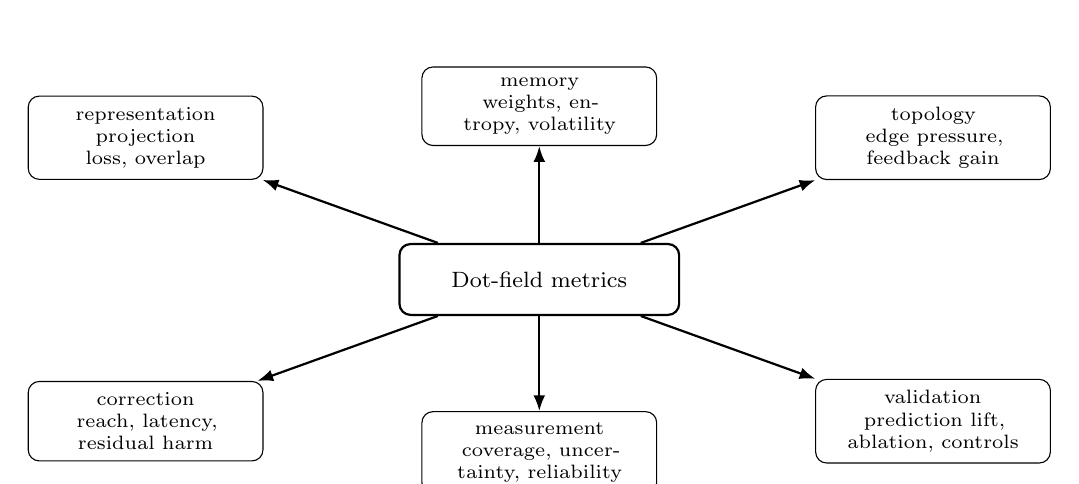
\begin{tikzpicture}[
  x=1cm,y=1cm,
  core/.style={draw, rounded corners, thick, align=center, text width=3.2cm, minimum height=0.9cm, font=\footnotesize, inner sep=5pt},
  fam/.style={draw, rounded corners, align=center, text width=2.7cm, minimum height=0.85cm, font=\scriptsize, inner sep=4pt},
  arr/.style={-{Latex[length=2mm]}, thick}
]
\node[core] (m) at (0,0) {Dot-field metrics};
\node[fam] (rep) at (-5,1.8) {representation\\projection loss, overlap};
\node[fam] (mem) at (0,2.2) {memory\\weights, entropy, volatility};
\node[fam] (top) at (5,1.8) {topology\\edge pressure, feedback gain};
\node[fam] (corr) at (-5,-1.8) {correction\\reach, latency, residual harm};
\node[fam] (meas) at (0,-2.2) {measurement\\coverage, uncertainty, reliability};
\node[fam] (val) at (5,-1.8) {validation\\prediction lift, ablation, controls};
\foreach \x in {rep,mem,top,corr,meas,val}{\draw[arr] (m) -- (\x);}
\end{tikzpicture}%
}
\caption{Metrics dashboard. The metric families track different parts of the theory: representation, memory dynamics, topology feedback, correction, measurement quality, and validation performance. No single metric validates the theory by itself.}
\label{fig:metrics-dashboard}
\end{figure}


\subsection{Dot weight}\label{dot-weight}

The weight of dot $d$ for agent $i$ at time $t$ is
\[
m_i(d,t).
\]
The interpretation of this quantity depends on the model. In a psychological model it may represent subjective salience, belief strength, or retrieval probability. In an AI-agent model it may represent memory score, embedding-retrieval rank, or stored priority. In an organizational model it may represent the practical force of a record, such as the degree to which a policy, incident report, or reputation trace is likely to be used in a future decision.

Dot weight should therefore be reported with its operational definition. A study should not treat $m_i(d,t)$ as directly observed unless the system actually records memory weights or retrieval scores. In most empirical settings it is an estimated latent variable or a proxy derived from recency, repetition, source credibility, access logs, retrieval logs, or explicit citation.

\subsection{Dot overlap}\label{dot-overlap}

Dot overlap measures shared access rather than shared belief. For two agents,
\[
Overlap(i,j,t)=\frac{|\mathcal M_i(t)\cap \mathcal M_j(t)|}{|\mathcal M_i(t)\cup \mathcal M_j(t)|}.
\]
A high value means that the two agents can access many of the same dots. It does not imply that they assign the same credibility, salience, valence, or interpretation to those dots. Two agents may share access to the same accusation and correction while trusting different sources or retrieving different parts of the lineage.

For this reason, dot overlap is best used with weighted similarity, credibility measures, and retrieval measures. In applications, overlap is useful for studying coordination, shared context, and common ground; it is insufficient by itself for studying agreement, polarization, or trust.

\subsection{Weighted dot similarity}\label{weighted-dot-similarity}

Let $m_i(t)$ and $m_j(t)$ be vectors of dot weights over a common reference vocabulary. Weighted similarity can be measured by cosine similarity:
\[
Sim(i,j,t)=\frac{m_i(t)\cdot m_j(t)}{\|m_i(t)\|\|m_j(t)\|}.
\]
Unlike simple overlap, this metric accounts for the relative strength of shared dots. It distinguishes agents who merely have access to the same traces from agents for whom those traces have comparable practical force.

The metric requires a common dot identity scheme. When two agents hold mutated or compressed descendants of the same source dot, the analyst must specify whether similarity is computed at token identity, lineage identity, or semantic identity. This choice can materially affect estimates of convergence and fragmentation.

\subsection{Fragmentation index}\label{fragmentation-index-metric}

The fragmentation index is most useful when the component partition is substantively justified. Components may be defined by observed social clusters, institutional units, platform communities, language groups, or algorithmic exposure regimes. If the partition is chosen after inspecting dot differences, the metric risks circularity. A strong study therefore defines the partition before measuring fragmentation or uses sensitivity analysis across multiple plausible partitions.


For a component partition $\mathcal{C}=\{C_1,\ldots,C_q\}$, define a
finite-time component summary $\bar m_r(t)$, for example the arithmetic
mean of dot-weight vectors inside $C_r$. A simple between-component
fragmentation metric is
$$
\mathcal{F}_{\mathcal{C}}(t)
=
\frac{2}{q(q-1)}\sum_{1\leq r<s\leq q}
\|\bar m_r(t)-\bar m_s(t)\|.
$$
High values indicate that component-level memories are far apart. This
metric should be interpreted alongside within-component convergence: an
echo chamber is not just high separation, but high internal similarity
combined with high external separation.

\subsection{Temporal sequencing sensitivity}\label{temporal-sequencing-sensitivity}

Temporal sequencing sensitivity should be evaluated on the same multiset of dots under different admissible orders. It is not enough to compare groups that saw different information. The distinctive claim is that order itself can matter when assimilation, correction, institutionalization, or bridge transmission is non-commutative. In empirical settings, this metric is strongest when sequence variation is induced experimentally or arises from plausibly exogenous timing differences.


For a sequence of dots $\mathbf d=(d_1,\ldots,d_L)$, define the
sequencing sensitivity of update rule $\chi$ at state $M$ as
$$
\mathcal{S}_\chi(M,\mathbf d)
=
\max_{\sigma,\sigma'}
\left\|M[\sigma(\mathbf d)]-M[\sigma'(\mathbf d)]\right\|.
$$
If $\mathcal{S}_\chi(M,\mathbf d)=0$, the sequence is order-insensitive
at $M$. If it is positive, ordering changes the resulting memory state.
A pairwise version is the commutator gap
$$
\mathcal{K}_{d,e}(M)
=
\Delta\big(F_e(F_d(M)),F_d(F_e(M))\big).
$$
This metric is useful for measuring framing effects, correction timing,
bridge timing, and early-versus-late institutional announcements.

\subsection{Institutional stabilization metrics}\label{institutional-stabilization-metrics}

Institutional dots require metrics that distinguish persistence, access,
authority, and dependence.

The \textbf{institutional persistence ratio} of a dot is
$$
IPR(d)=\frac{\lambda_I(d)}{\lambda_P(d)}.
$$
Values greater than one indicate that institutional encoding slows decay
relative to private memory.

The \textbf{archival reach} of an institutional dot is
$$
AR(d,t)=\frac{1}{|A|}\sum_{i=1}^{|A|}\mathbf 1\{(a_i,d^I)\in B_t^I\}.
$$
This measures how much of the agent population can access the dot
through the institution.

The \textbf{effective institutional strength} of a dot for an agent is
$$
EIS_i(d,t)=b_i^I(d,t)\gamma_i^I(d,t)m_i^I(d,t).
$$
This is the institutional version of effective retrievable strength.

The \textbf{institutional dependence} of a group is
$$
ID_G(t)=
\frac{\sum_{i\in G}\sum_{d\in D_t^I}Q_i^I(d,t)}
{\sum_{i\in G}\sum_{d\in D_t^I\cup D_t^P}Q_i(d,t)}.
$$
High institutional dependence means that the group's actionable memory
is strongly mediated by institutional stores. This may improve
coordination and persistence, but it also increases exposure to
institutional capture risk.

\subsection{Topology-feedback metrics}\label{topology-feedback-metrics}

Dot-induced topology requires metrics that connect retrieved traces to
edge change.

The \textbf{edge pressure} from $a_i$ to $a_j$ is
$$
\zeta_{ij}(t)=
\sum_{d\in \mathcal V_i(q_{ij},t):\,T(d)=a_j}
\omega_i(d,t)v_i(d,j,t).
$$
Positive values indicate trust-building pressure; negative values
indicate trust-eroding pressure.

The \textbf{edge-pressure imbalance} is
$$
EPI_{ij}(t)=\zeta_{ij}^{+}(t)-\zeta_{ij}^{-}(t).
$$
This is useful when positive and negative dots coexist.

The \textbf{dot-mediated reputation score} of $a_j$ is
$$
Rep_j(t)=\sum_{i\neq j}\rho_i(t)w_{ij}(t).
$$
Source-weighted reputation can be compared against unweighted incoming
trust to detect whether reputation is concentrated in high-status
sources or broadly distributed.

The \textbf{dot-to-edge elasticity} of dot $d$ on edge $i\to j$ is
$$
DEE_{ij,d}(t)=
\left|\frac{\partial w_{ij}(t+1)}{\partial v_i(d,j,t)}\right|
=\eta\psi'(\zeta_{ij}(t))\omega_i(d,t),
$$
whenever $\psi$ is differentiable and $d$ contributes linearly to
$\zeta_{ij}(t)$. High elasticity means a small change in the dot's valence or
interpretation can produce a large edge update.

The \textbf{reputation volatility} of $a_j$ is
$$
RV_j(t)=|Rep_j(t+1)-Rep_j(t)|.
$$
High volatility indicates that the agent's reputation is unstable or
sensitive to new dots.

The \textbf{exclusion risk} of $a_j$ at threshold $\tau$ is
$$
ER_j^\tau(t)=
\frac{1}{|A|-1}\sum_{i\neq j}\mathbf 1\{\psi(\zeta_{ij}(t))<\tau\}.
$$
This estimates the share of potential incoming ties whose dot pressure
points below the threshold for relation maintenance.

The \textbf{topology-memory coupling} over an interval is
$$
TMC(t)=corr\big(\zeta_{ij}(t),\Delta w_{ij}(t)\big),
$$
computed over ordered pairs. High positive coupling indicates that edge
updates are strongly aligned with dot-induced evaluative pressure.

\subsection{Counter-dot and epistemic resilience metrics}\label{counter-dot-and-epistemic-resilience-metrics}

Correction requires metrics that distinguish counter-dot existence from
counter-dot effectiveness.

The \textbf{effective counter-strength} of a counter-dot is
$$
CE_i(c,d,t)=Q_i(c,t)\kappa_i(c,d,t).
$$
It is zero when the counter-dot is inaccessible, unretrieved, untrusted,
or poorly matched to the target dot.

The \textbf{correction pressure} on target dot $d$ for agent $a_i$ is
$$
C_i^{eff}(d,t)=\eta_i\sum_{c\in C_i(d,t)}CE_i(c,d,t).
$$
This is the quantity that must exceed reinforcement load for correction
to proceed.

The \textbf{reinforcement load} of a target dot is
$$
L_i(d,t),
$$
representing repetition, social validation, institutional persistence,
algorithmic ranking, emotional salience, or identity attachment.

The \textbf{correction surplus} is
$$
CS_i(d,t)=C_i^{eff}(d,t)-L_i(d,t).
$$
Positive values indicate that correction pressure exceeds the load
sustaining the target dot.

The \textbf{group error mass} for a disputed dot is
$$
E_G(d,t)=\sum_{i\in G}e_i(d,t).
$$
The \textbf{maximum error margin} is
$$
E_G^{\infty}(d,t)=\|\mathbf e_d(t)\|_\infty.
$$

The \textbf{correction reach} of a counter-dot is
$$
CR(c,d,t)=\frac{1}{|G|}\sum_{i\in G}\mathbf 1\{CE_i(c,d,t)>0\}.
$$
This measures how many agents can use the counter-dot effectively, not
merely how many could theoretically view it.

The \textbf{correction latency} is
$$
T_{corr}^{G}(d,\varepsilon)=
\inf\{k\geq0:\|\mathbf e_d(t_0+k)\|_\infty\leq\varepsilon\}.
$$

The \textbf{residual topology harm} to target agent $a_j$ is
$$
RTH_j(t)=\sum_{i\neq j}\big[w_{ij}^{pre}-w_{ij}^{post}\big]_+.
$$
This captures unrepaired relational loss after a dot has been corrected.

A simple \textbf{epistemic resilience index} for group $G$ against dot
$d$ is
$$
ERI_G(d,t)=
\frac{1+\sum_{i\in G}C_i^{eff}(d,t)}
{1+\sum_{i\in G}L_i(d,t)+E_G(d,t)+RTH_G(t)}.
$$
Higher values indicate stronger correction capacity relative to
reinforcement load, current error, and residual topology harm. This is a
measurement proposal rather than a theorem; its empirical usefulness
should be tested against correction outcomes.

\subsection{Mutation, drift, and compression metrics}\label{mutation-drift-and-compression-metrics}

Mutation and compression require metrics that distinguish faithful
transmission from semantic distortion and useful summarization from
harmful simplification.

The \textbf{semantic distance} between two dots is
$$
SD(d,e)=\Delta_{\mathcal X}(x(d),x(e)).
$$

The \textbf{lineage drift} from ancestor $d_0$ to descendant $d_L$ is
$$
LD_{\mathcal X}(d_0,d_L)=\Delta_{\mathcal X}(x(d_0),x(d_L)).
$$

The \textbf{mutation rate} of a lineage is
$$
MR_{\mathcal X}(\mathcal L)=\frac{1}{L}
\sum_{\ell=0}^{L-1}
\Delta_{\mathcal X}(x(d_{\ell}),x(d_{\ell+1})).
$$

A simple \textbf{semantic fidelity score} is
$$
SF(d_0,d_L)=\frac{1}{1+LD_{\mathcal X}(d_0,d_L)}.
$$
Higher values indicate greater semantic preservation.

The \textbf{compression ratio} for a source set $S$ is
$$
CompR_i(S)=\frac{|S|}{|C_i(S)|},
$$
where $|C_i(S)|$ is the number of compressed dots produced. In the
single-summary case, $CompR_i(S)=|S|$.

The \textbf{behavioral compression loss} for a decision class $\Pi$ is
$$
BCL_i(S)=\sup_{\pi\in\Pi}
\left\|P_{\pi}(\cdot\mid S)-P_{\pi}(\cdot\mid C_i(S))\right\|_1.
$$
Low behavioral compression loss means the summary preserves what matters
for action. High loss means the summary erases action-relevant detail.

The \textbf{summary dominance ratio} is
$$
SDR_i(d_S^\star,S,t)=\frac{Q_i(d_S^\star,t)}{\sum_{d\in S}Q_i(d,t)}.
$$
Values above one indicate that the summary dot is stronger in retrieval
than all source dots combined.

The \textbf{semantic counter-fit mismatch} between counter-dot $c$ and
mutated target $d'$ is
$$
SCM_i(c,d',t)=1-\kappa_i(c,d',t).
$$
High mismatch predicts correction difficulty.

The \textbf{semantic brokerage capital} proxy is
$$
SBC_i(t)=\sum_{d\in D_t}
\beta_i(d,t)Reach_i(d,t)Value_i(d,t)Fidelity_i(d,t).
$$
This measures the value of controlling or authenticating transformations
of dots across social boundaries.

\subsection{Identifiability and empirical estimation metrics}\label{identifiability-and-empirical-estimation-metrics}

Dot-field estimation requires metrics that assess whether the inferred
trace structure is observable, stable, and useful.

The \textbf{dot observation coverage} in a simulation or audited dataset
is
$$
DOC(t)=\frac{|\widehat D_t\cap D_t|}{|D_t|},
$$
where $D_t$ is the ground-truth dot set and $\widehat D_t$ is the
estimated dot set. In real datasets without ground truth, this can be
approximated through audits, duplicated coding, or known institutional
records.

The \textbf{provenance completeness} of a dot is
$$
PC(d)=\frac{\#\{\text{observed required provenance fields for }d\}}
{\#\{\text{required provenance fields for }d\}}.
$$
Required fields may include source, witness, timestamp, context,
transmission path, institution, and version.

The \textbf{access observability} of a study is
$$
AO(t)=\frac{|\widehat B_t\cap B_t|}{|B_t|},
$$
in simulation, or the audited share of access events captured by logs in
empirical data.

The \textbf{dot-relation reconstruction score} is
$$
DRR(t)=1-\frac{\|\widehat R_t^D-R_t^D\|_1}{\max(1,\|R_t^D\|_1)},
$$
when a ground-truth or audited relation matrix is available.

The \textbf{edge-pressure reconstruction error} is
$$
PRE(t)=\frac{1}{|E_t|}\sum_{(i,j)\in E_t}
\left|\widehat \zeta_{ij}(t)-\zeta_{ij}(t)\right|.
$$
Low values indicate that estimated dots recover the aggregate pressure
that drives social-edge updates.

The \textbf{identifiability ambiguity set} for estimand $g$ is
$$
Amb_g(Y)=\{g(\Omega_{0:T},\theta):(\Omega_{0:T},\theta)\text{ is compatible with }Y\}.
$$
When $Amb_g(Y)$ contains one value, $g$ is identified. When it contains
many values, the data underdetermine the estimand.

The \textbf{rank adequacy ratio} for dot-action coefficient estimation is
$$
RAR=\frac{\operatorname{rank}(X)}{K},
$$
where $X$ is the dot-feature design matrix and $K$ is the number of dot
features. A value of one is necessary for full-rank coefficient
identification in the linear-index model.

The \textbf{dot-field prediction lift} is
$$
PL_D=S(\mathcal M_D)-S(\mathcal M_0)
$$
for scores where larger is better, or
$$
PL_D=L(\mathcal M_0)-L(\mathcal M_D)
$$
for losses where smaller is better. This measures whether dot-field
features improve held-out prediction over an agent-edge baseline.

The \textbf{interventional leverage} of a dot exposure experiment is
$$
IL_d=\left|\mathbb E[Y\mid do(B_{id}=1)]-\mathbb E[Y\mid do(B_{id}=0)]\right|.
$$
High interventional leverage indicates that controlled dot exposure has
a strong causal effect on the chosen outcome.


\subsection{Extraction and coding quality metrics}\label{extraction-coding-quality-metrics}

Extraction quality metrics should be reported separately for dot detection, attribute coding, access coding, relation coding, and lineage coding. A high dot-detection score does not imply that the access graph is accurate, and a reliable valence code does not imply reliable semantic identity. Treating extraction quality as one number can hide the measurement weakness most relevant to the claim being tested.


The quality of a dot-field dataset should be reported alongside substantive dot metrics. The \textbf{dot detection F1} is
\[
F1_D=\frac{2TP_D}{2TP_D+FP_D+FN_D}.
\]
The \textbf{relation extraction F1} is
\[
F1_R=\frac{2TP_R}{2TP_R+FP_R+FN_R}.
\]
The \textbf{attribute completeness score} for dot \(d\) is
\[
ACS(d)=\frac{\#\{\text{observed or justified required fields for }d\}}
{\#\{\text{required fields for }d\}}.
\]
The \textbf{access uncertainty mass} is
\[
AUM(t)=\sum_{i,d}\widehat B_{id}(t)(1-\widehat B_{id}(t)),
\]
which is largest when access probabilities are near one half and smallest when access is known. The \textbf{outcome-blind coding rate} is
\[
OBR=\frac{\#\{\text{dots coded before outcome inspection}\}}
{\#\{\text{coded dots}\}}.
\]
Low values warn that extraction may be contaminated by outcome knowledge. The \textbf{observability grade} \(O\in\{0,1,2,3,4,5\}\) should be reported for each dataset or sub-study using the ladder in Table~\ref{tab:measurement-observability-ladder}.

\subsection{Algorithmic implementation metrics}\label{algorithmic-implementation-metrics}

Executable dot-field systems require metrics for computational fidelity,
scalability, and approximation quality.

The \textbf{state validity violation count} is
$$
SVC(t)=\#\{\text{violated implementation invariants at time }t\}.
$$
A correct implementation should maintain $SVC(t)=0$ except in deliberately
simulated failure conditions.

The \textbf{implementation transition divergence} is
$$
ITD(t)=\mathsf D\left(P_{\mathcal A}(\widehat\Omega_{t+1}\mid\widehat\Omega_t),
\mathsf K(\cdot\mid\widehat\Omega_t)\right),
$$
where $\mathsf D$ may be total variation, Wasserstein distance,
Kullback-Leibler divergence, or a task-specific state-distance metric.

The \textbf{retrieval recall at $k$} is
$$
RR@k=\frac{|R_i^{exact}(q,t)\cap R_i^{approx,k}(q,t)|}{|R_i^{exact}(q,t)|},
$$
computed when exact retrieval is feasible or on audited samples.

The \textbf{retrieval feature error} is
$$
RFE_i(q,t)=\|h_i(R_i^{exact})-h_i(R_i^{approx})\|.
$$
This is more action-relevant than set overlap when different retrieved
sets induce similar aggregate decision features.

The \textbf{truncated dot mass} for agent $a_i$ is
$$
TDM_i(t)=\left\|\sum_{d\in G_i(t)}Q_i(d,t)\varphi(d)\right\|,
$$
where $G_i(t)$ is the set of ignored, dropped, archived, or unscreened
dots.

The \textbf{runtime per transition} is
$$
RT(t)=\text{wall-clock time required to compute }\widehat\Omega_{t+1}.
$$
The \textbf{memory footprint} is
$$
MF(t)=\text{bytes used to store }\widehat\Omega_t.
$$
Both should be reported with $n$, $m$, $e_A$, $e_D$, $b$, $k$, and event
batch size.

The \textbf{dot churn rate} is
$$
DCR(t)=\frac{|D_{t+1}\triangle D_t|}{\max(1,|D_t|)},
$$
where $\triangle$ denotes symmetric difference. High churn indicates
rapid dot creation, deletion, mutation, or canonicalization instability.

The \textbf{auditability score} is
$$
AUD(t)=\frac{\#\{\text{state changes with recorded provenance}\}}{\#\{\text{state changes}\}}.
$$
High auditability means that actions, edge updates, corrections,
institutional writes, and dot mutations can be traced back to source
records.

\subsection{Executable simulator metrics}\label{executable-simulator-metrics}

The minimal simulator should also report metrics that measure whether a
run is scientifically useful, reproducible, and comparable to baselines.

\paragraph{Simulation reproducibility score.}
Let $r_j\in\{0,1\}$ indicate whether reproducibility item $j$ is
reported. Then
$$
SRS=\frac{1}{J}\sum_{j=1}^J r_j.
$$

\paragraph{Mechanism activation vector.}
Let
$$
\mathsf{MAV}=(m_{retr},m_{create},m_{trans},m_{mut},m_{corr},m_{inst},m_{edge})
$$
indicate whether retrieval, creation, transmission, mutation,
correction, institutionalization, and edge feedback are enabled. This
makes experimental conditions explicit.

\paragraph{Baseline prediction lift.}
For a dot-field simulator model $\mathcal M_D$ and baseline
$\mathcal M_B$,
$$
BPL_D=L(\mathcal M_B)-L(\mathcal M_D),
$$
where $L$ is a held-out loss. A positive value indicates improvement
over the baseline.

\paragraph{Trace audit coverage.}
Let $N_{events}$ be the number of simulated events and $N_{logged}$ the
number with complete actor, dot, parent, and state-change fields. Then
$$
TAC=\frac{N_{logged}}{N_{events}}.
$$

\paragraph{Theorem test pass rate.}
If $P_h\in\{0,1\}$ records whether theorem-mapped test $h$ passes, then
$$
TTPR=\frac{1}{H}\sum_{h=1}^H P_h.
$$

\paragraph{Run divergence under ablation.}
For full model trajectory $\Gamma_D$ and ablated trajectory $\Gamma_A$,
$$
RDA=Dist(\Gamma_D,\Gamma_A),
$$
where $Dist$ may be final graph distance, dot-weight distance, action
sequence distance, or metric-trajectory distance. This measures which
mechanisms materially change simulated social history.


\subsection{Mixed-mechanism dynamics metrics}\label{mixed-mechanism-dynamics-metrics}

Mixed-mechanism metrics are intended to detect interaction effects. A high mechanism activation density means that many operators are active, but it does not prove that they interact. Mechanism-order sensitivity, composed Lipschitz bounds, and matched-run ablations help determine whether combined dynamics generate behavior not reducible to independent single-mechanism effects.


For the integrated dynamics model, useful metrics include the mechanism activation vector
\[
\mathbf a_t=(a_R,a_A,a_K,a_T,a_U,a_C,a_I,a_H,a_L,a_E),
\]
the mechanism activation density
\[
MAD(t)=\frac{1}{10}\sum_{s=1}^{10}a_s(t),
\]
the composed Lipschitz bound
\[
LCB(t)=\prod_{s:a_s(t)=1}L_s(t),
\]
the feedback gain for topology-access-memory recursion
\[
G_{fb}(t)=b_E(t)\zeta_B(t)e_\zeta(t),
\]
and the mechanism-order sensitivity
\[
MOS_{a,b}(t)=d_\Omega\big(\mathscr G_b\mathscr G_a(\Omega_t),\mathscr G_a\mathscr G_b(\Omega_t)\big).
\]
High activation density means the model is using many mechanisms and therefore needs stronger measurement support. An \(LCB\) below one suggests conservative stability under the chosen metric. An \(LCB\) or feedback gain above one flags possible amplification, cascades, or lock-in. Positive \(MOS\) indicates that update order is substantively consequential rather than a harmless implementation detail.

\subsection{Recursive topology-feedback stability metrics}\label{recursive-topology-feedback-stability-metrics}

Recursive stability metrics should be interpreted locally unless global contraction has been established. A positive stability margin near one equilibrium does not guarantee stability after a large shock or after access thresholds change. Shock amplification ratios, bridge recovery margins, and access-closure risk therefore complement the Jacobian condition by showing how the system behaves under finite perturbations.


For the recursive topology-feedback loop, useful diagnostics include the local feedback Jacobian
\[
J_\Theta(t)=E_e(t)+E_\zeta(t)\zeta_r(t)R_b(t)B_e(t),
\]
the recursive stability margin
\[
SM(t)=1-\rho(J_\Theta(t)),
\]
the access-closure risk
\[
ACR_{ij}(t)=\mathbf 1\{w_{ij}(t)<\tau_B,\ \theta_{ij}^{closed}(t)<\tau_B\},
\]
the bridge recovery margin
\[
BRM_{ij}(t)=\theta_{ij}^{bridge}(t)-\tau_B,
\]
and the shock amplification ratio
\[
SAR(k)=\frac{\|e_{t+k}^{pert}-e_{t+k}^{base}\|}{\|e_t^{pert}-e_t^{base}\|}.
\]
Positive \(SM\) indicates local damping; negative \(SM\) indicates local amplification. High \(ACR\) flags relations at risk of self-sealing closure. Positive \(BRM\) indicates that bridge or institutional correction is strong enough, if sustained, to recover an access channel. \(SAR(k)>1\) indicates finite-horizon amplification of a topology perturbation.


\subsection{Collective memory convergence}\label{collective-memory-convergence}

Collective memory convergence should not be equated with truth or desirability. A group can converge on an accurate record, a misleading rumor, a simplified stereotype, or an institutional error. The convergence metric measures alignment of accessible or weighted dots; interpretation requires credibility, contradiction, correction, and provenance measures. This distinction keeps the theory truth-neutral while still allowing normative evaluation.


Collective memory convergence measures the extent to which members of a group carry similar weighted dot fields. For group $G$, one simple measure is
\[
CMC(G,t)=\frac{1}{|G|(|G|-1)}\sum_{i\neq j}Sim(i,j,t).
\]
High $CMC$ indicates that agents assign similar weights to the relevant dot vocabulary. This does not necessarily mean that the group is accurate, normatively desirable, or epistemically healthy. A group can converge on true records, false rumors, institutional errors, or simplified narratives. For this reason, convergence should be interpreted alongside contradiction ratio, provenance quality, correction reach, and external validation where available.

\subsection{Social-dot coupling}\label{social-dot-coupling}

Social-dot coupling measures whether social proximity and dot similarity move together. High coupling may indicate shared context and coordination, but it can also indicate echo-chamber formation or exclusionary information flow. Low coupling may indicate diverse exposure, weak shared memory, or a platform-mediated environment in which algorithmic access overrides interpersonal ties. The metric should therefore be interpreted with the topology and access mechanism in view.


Social-dot coupling measures whether social proximity and memory similarity move together:
\[
SDC(t)=corr(w_{ij}(t),Sim(i,j,t)).
\]
A high value indicates that socially close agents remember similarly, either because ties transmit dots or because shared dots create or preserve ties. The correlation alone does not identify the direction of causality. To distinguish social selection from social influence, the analyst should use temporal ordering, edge-update models, interventions, or lagged comparisons.

\subsection{Dot centrality}\label{dot-centrality}

Dot centrality measures the structural importance of a trace inside the dot graph $G^D_t$ or the lifted heterogeneous graph $H_t$. In $G^D_t$, degree centrality captures how many other dots support, contradict, cite, or summarize a dot. Betweenness centrality captures whether a dot mediates paths between clusters of memory. Eigenvector or PageRank-like centrality captures whether a dot is connected to other influential dots. In $H_t$, a dot may also become central because many agents access it through $B_t$.

Centrality should not be confused with truth or value. A false accusation, viral rumor, or obsolete policy may be highly central. The relevant empirical question is whether central dots influence retrieval, action, correction cost, or topology change.

\subsection{Dot entropy}\label{dot-entropy}

Dot entropy is useful for diagnosing concentration. Low entropy indicates that an agent's practical memory is dominated by a small number of traces, which may support coordination when those traces are accurate and shared, or create vulnerability when they are false, traumatic, or institutionally biased. High entropy indicates a diverse memory field, but it may also create retrieval instability if the agent lacks mechanisms for prioritization and compression.


Dot entropy measures the concentration of an agent's memory weight:
\[
H_i(t)=-\sum_{d\in \mathcal M_i(t)}p_i(d,t)\log p_i(d,t),
\]
where $p_i(d,t)$ is the normalized weight assigned by agent $i$ to dot $d$. Low entropy means that a few dots dominate retrieval and action. High entropy indicates a more distributed memory field. Low entropy can be efficient when the dominant dots are reliable and task-relevant; it can be risky when a single salient trace crowds out counter-evidence or nuance.

\subsection{Dot volatility}\label{dot-volatility}

Dot volatility is a useful early-warning measure. Rapid changes in credibility, salience, access, or valence may signal active controversy, correction, rumor spread, institutional revision, or semantic drift. Volatility should be decomposed by attribute whenever possible, because a dot can be stable in content but volatile in credibility, or stable in access but volatile in interpretation.


Dot volatility measures the rate at which a dot's weight or effective strength changes:
\[
V_d(t)=|m(d,t+1)-m(d,t)|.
\]
High volatility indicates that a dot is unstable, newly introduced, actively contested, or being rapidly reinforced or corrected. Low volatility indicates stability, consolidation, neglect, or institutional anchoring. Volatility should be evaluated with lifecycle state: a stable dot may be stable because it is accepted, forgotten, or institutionally fixed.

\subsection{Contradiction ratio}\label{contradiction-ratio}

The contradiction ratio should be interpreted with caution. A high ratio may indicate polarization, contested evidence, active correction, or healthy epistemic pluralism. A low ratio may indicate consensus, but it may also indicate suppressed counter-dots or poor measurement. The metric is most informative when paired with reach, source credibility, and whether contradiction edges connect across components or remain confined within separate communities.


The contradiction ratio measures contestation in the dot graph:
\[
CR(t)=\frac{\#\{(d,e)\in R_t^D: d\dashv e\}}{\#\{(d,e)\in R_t^D\}}.
\]
High contradiction ratio indicates a contested memory field. This can be epistemically healthy when disagreement exposes error and permits correction. It can also indicate fragmentation when contradictions are separated by group, source, or access boundary. The metric should therefore be interpreted together with correction reach and component-level fragmentation.

\subsection{Dot half-life}\label{dot-half-life}

Dot half-life is mechanism-specific. A private memory half-life, institutional archive half-life, retrieval half-life, and reputational half-life may differ substantially. Reporting a single half-life can conceal whether a trace persists materially, psychologically, institutionally, or socially. A mature analysis should specify which strength variable is decaying and what event counts as reinforcement.


The half-life of a dot is the time required for its weight or effective strength to fall to half its initial value:
\[
m(d,t+k)=\frac{1}{2}m(d,t).
\]
In an exponential decay model $m(d,t+k)=\lambda^k m(d,t)$, the half-life is
\[
k_{1/2}=\frac{\log(1/2)}{\log(\lambda)}.
\]
Comparing half-lives across private, social, and institutional dots measures stabilization. A long half-life can be beneficial for reliable commitments, laws, and archives; it can be harmful for false accusations, obsolete records, or institutional errors.

\subsection{Dot-mediated social capital score}\label{dot-mediated-social-capital-score}

A dot-mediated social capital score should not be treated as a universal scalar unless the utility context is specified. Access to a technical incident archive may be valuable in an engineering organization and irrelevant in a different community. A useful score therefore defines a utility-relevant domain, a set of valuable dots, an access and retrieval model, and a liability model for harmful or exclusionary traces. The score is best reported as a decomposition into bonding, bridging, reputation, archival access, semantic brokerage, correction capacity, and liability rather than as a single opaque index.


A practical empirical score for agent \(a_i\) can combine social
position, dot access, reputation, and liabilities: \[
DMSC_i(t)=
\omega_1 Degree_i(t)+
\omega_2 Bridge_i(t)+
\omega_3 \sum_{d\in \mathcal M_i(t)} val_i(d,t)+
\omega_4 PosRep_i(t)-
\omega_5 NegRep_i(t).
\] This measure is not intended to replace established social capital
measures. It is a dot-field operationalization useful for simulations
and AI-agent systems.

\subsection{Validation and benchmarking metrics}\label{validation-and-benchmarking-metrics}

The \textbf{empirical prediction lift} of a dot-field model over a baseline is
\[
\widehat{PL}_D=\frac{1}{R}\sum_{r=1}^R\left(\ell_0(r)-\ell_D(r)\right).
\]
Positive values indicate lower average loss for the dot-field model on the same
prediction instances.

The \textbf{baseline separation score} over a set of baselines
\(\mathcal B\) is
\[
BSS_D=\min_{b\in\mathcal B}\left(L(\widehat{\mathcal M}_b)-L(\widehat{\mathcal M}_D)\right).
\]
A positive value means the dot-field model beats every specified baseline.

The \textbf{run divergence under ablation} for mechanism \(m\) is
\[
RDA_m=\frac{1}{S}\sum_{s=1}^{S}
\Delta\big(\tau_s^{full},\tau_s^{(-m)}\big).
\]
This measures whether a named mechanism materially changes trajectories under
matched simulation conditions.

The \textbf{negative-control degradation} for control \(c\) is
\[
NCD_c=L(\widehat{\mathcal M}_{D,c})-L(\widehat{\mathcal M}_{D}).
\]
A positive value means performance declined when the relevant dot structure was
destroyed.

The \textbf{temporal generalization gap} is
\[
TGG=L_{future}(\widehat{\mathcal M})-L_{validation}(\widehat{\mathcal M}).
\]
Large values indicate that the model fits historical dot patterns but fails to
generalize forward.

The \textbf{mechanism-specific theorem pass rate} is
\[
MTPR_m=\frac{\#\{\text{runs where theorem signature for }m\text{ is observed}\}}
{\#\{\text{eligible runs}\}}.
\]
This metric should be reported with the theorem assumptions that made a run
eligible.

The \textbf{leakage audit gap} is
\[
LAG=L(\widehat{\mathcal M}_{valid})-L(\widehat{\mathcal M}_{future\ oracle}).
\]
A very large gap is not a target for improvement; it is a warning that future
information can easily inflate performance and that the valid pipeline must be
carefully audited.


\subsection{Simulator calibration metrics}\label{simulator-calibration-metrics}

Calibration metrics connect the simulator to its claim strength. A low calibration loss indicates that chosen summaries match targets, but the calibration tier determines what kind of conclusion is justified. Design calibration supports mechanism illustration; signature calibration supports theorem demonstrations; distributional calibration supports stylized empirical comparison; predictive calibration supports stronger out-of-sample claims. The calibration overfit gap should always be reported when parameters are chosen from observed targets.


Simulator calibration introduces additional diagnostics. The \textbf{calibration loss} is
\[
CAL(\theta)=\sum_{r=1}^{R}\omega_r\,\Delta_r\big(s_r^{sim}(\theta),s_r^{target}\big)^2.
\]
The \textbf{parameter sensitivity index} for parameter $\theta_j$ and summary $s_r$ is
\[
PSI_{rj}=\left|\frac{\partial s_r^{sim}(\theta)}{\partial \theta_j}\right|,
\]
estimated by finite differences when analytic derivatives are unavailable. The \textbf{calibration overfit gap} is
\[
COG=CAL_{holdout}(\widehat\theta)-CAL_{calib}(\widehat\theta).
\]
Large positive values indicate that calibration matched the calibration targets but failed to generalize to held-out summaries. The \textbf{calibration tier} is
\[
CT\in\{C0,C1,C2,C3\},
\]
where higher tiers support stronger claims only when leakage controls and negative controls are passed.


\section{Empirical Hypotheses}\label{research-hypotheses}

The formal results above imply empirical hypotheses only when the corresponding mechanisms are active and measurable in a given domain. This section groups the hypotheses by mechanism family rather than treating them as isolated claims. Each family identifies the expected empirical signature, the most relevant observability requirement, and a negative-control condition that should weaken or eliminate the effect. The hypotheses are therefore intended as a bridge between theory and study design, not as universal laws.

\begin{longtable}[]{@{}L{0.20\textwidth}L{0.33\textwidth}L{0.27\textwidth}L{0.15\textwidth}@{}}
\toprule
Hypothesis family & Core prediction & Empirical signature & Principal negative control\\
\midrule
\endhead
Dot-mediated social capital & Agents with better access to valuable dots, stronger reputational support, stronger bridging positions, and lower dot liabilities obtain greater actionable advantage. & Higher task success, cooperation probability, influence, or recovery speed conditional on comparable non-dot attributes. & Shuffle access or provenance while preserving edge degree.\\
Temporal sequencing & Groups exposed to the same dots in different orders can converge to different memory states when assimilation operators do not commute. & Order-sensitive divergence in dot weights, interpretations, or later actions. & Randomize sequence labels or use commuting assimilation tasks.\\
Institutional stabilization & Institutional dots persist longer, reach more agents, and are harder to correct than private dots. & Longer half-life, larger reach, higher correction threshold, and stronger synchronization. & Replace institutional source labels with private-source labels while preserving content.\\
Topology and reputation & Evaluative dots predict trust-edge change, reputation trajectories, alliance formation, and exclusion risk. & Edge updates correlate with retrieved evaluative pressure beyond prior edge state. & Target shuffle or valence shuffle.\\
Correction and resilience & Counter-dot effectiveness depends on access, credibility, semantic fit, and reinforcement load. & Faster correction when counter-strength and correction reach are high. & Counter-dot mismatch or access removal.\\
Mutation and compression & Multi-hop transmission and high compression create drift, simplification, and correction mismatch. & Larger semantic distance, summary dominance, and behavioral compression loss. & Anchor all transmissions to a canonical record.\\
Identifiability and validation & Rich provenance, access, and retrieval data identify dot-field quantities better than action-only data. & Higher prediction lift, lower reconstruction ambiguity, lower edge-pressure error. & Remove provenance/access logs.\\
Implementation and scalability & Sparse top-$k$ retrieval and bounded-memory truncation preserve behavior when omitted dot mass is low. & Small behavioral divergence with lower runtime and memory footprint. & Truncate high-impact dots rather than low-impact dots.\\
Mixed-mechanism feedback & Interacting mechanisms produce amplification or stability depending on composed gain and Jacobian margin. & Shock amplification when feedback gain exceeds stability margin; damping when below it. & Ablate the dominant feedback channel.\\
Calibration and reproducibility & Higher calibration tiers support stronger claims only when overfit gaps remain small. & Stable mechanism signatures across seeds, graph structures, and held-out regimes. & Tune only to the target signature and test on new regimes.\\
\bottomrule
\end{longtable}

The hypotheses can also be expressed as five overarching empirical claims.

\textbf{H1: representational lift.} In memory-sensitive domains, dot-field features should improve prediction of future action, edge change, correction, or coordination relative to reduced agent-edge states. The expected signature is positive held-out prediction lift under temporal separation. The claim fails locally when
\[
I(Y_{t+1};D_t,R_t^D,B_t,\mathbf M_t,Q_t,L_t\mid Z_t)=0.
\]

\textbf{H2: mechanism specificity.} The source of dot-field lift should depend on the active mechanism. If reputation dynamics are active, evaluative dots should matter; if correction dynamics are active, counter-dot reach and fit should matter; if semantic drift is active, lineage and mutation measures should matter. Mechanism ablation should reduce the corresponding signature without necessarily eliminating all dot-field value.

\textbf{H3: negative-control discipline.} Dot-field advantages should weaken under destructive controls that preserve superficial complexity while breaking the relevant mechanism. Examples include target shuffling for reputation, access shuffling for exposure, temporal reversal for sequencing, lineage shuffling for mutation, and counter-dot mismatch for correction.

\textbf{H4: observability dependence.} Stronger dot-field claims require stronger observability. Action-only data may identify aggregate pressure but not dot composition. Provenance logs, access records, retrieval traces, institutional anchors, and randomized exposure increase identifiability and reduce ambiguity.

\textbf{H5: governance dependence.} In high-stakes domains, the value of a dot-field system should be evaluated not only by prediction or coordination but also by contestability, correction reach, proportional forgetting, privacy protection, and auditability. A system that predicts well but cannot explain, correct, or govern its traces is not a successful implementation of the theory.


\section{Simulation Program}\label{simulation-program}

The simulation program is organized as a benchmark suite rather than as a loose list of examples. Each benchmark activates a specific mechanism, includes a reduced baseline, and records a theorem-linked signature. Figure~\ref{fig:simulation-benchmark-suite} shows the intended progression from single-mechanism tests to integrated mixed-mechanism tests.




\begin{figure}[htbp]
\centering
\resizebox{0.98\textwidth}{!}{%
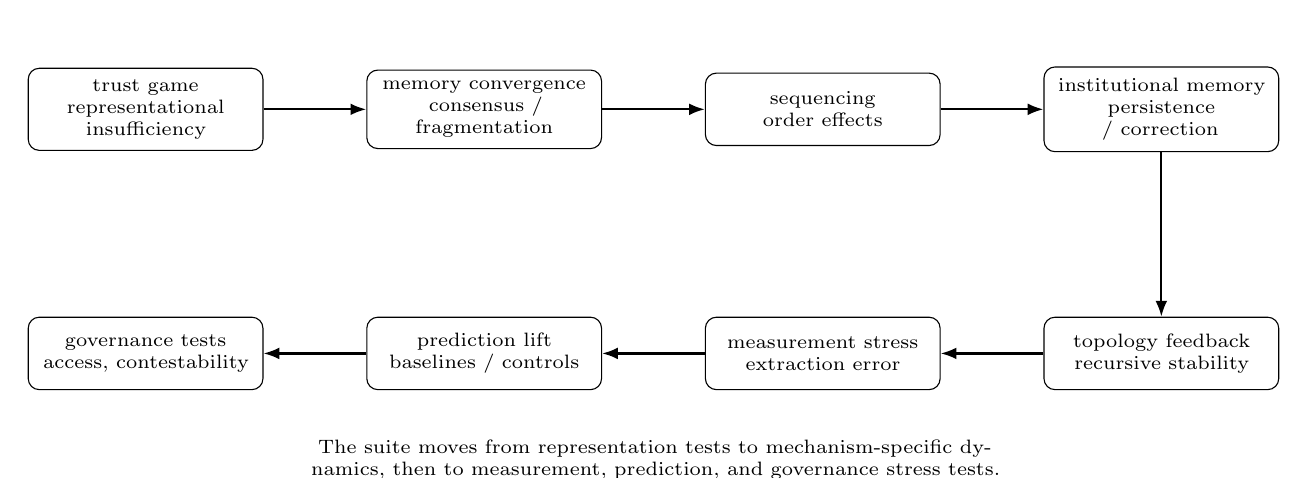
\begin{tikzpicture}[
  x=1cm,y=1cm,
  box/.style={draw, rounded corners, align=center, text width=2.70cm, minimum height=0.92cm, font=\scriptsize, inner sep=4pt},
  arr/.style={-{Latex[length=2mm]}, thick}
]
\node[box] (b1) at (0,1.55) {trust game\\representational insufficiency};
\node[box] (b2) at (4.3,1.55) {memory convergence\\consensus / fragmentation};
\node[box] (b3) at (8.6,1.55) {sequencing\\order effects};
\node[box] (b4) at (12.9,1.55) {institutional memory\\persistence / correction};
\node[box] (b5) at (12.9,-1.55) {topology feedback\\recursive stability};
\node[box] (b6) at (8.6,-1.55) {measurement stress\\extraction error};
\node[box] (b7) at (4.3,-1.55) {prediction lift\\baselines / controls};
\node[box] (b8) at (0,-1.55) {governance tests\\access, contestability};
\draw[arr] (b1.east) -- (b2.west);
\draw[arr] (b2.east) -- (b3.west);
\draw[arr] (b3.east) -- (b4.west);
\draw[arr] (b4.south) -- (b5.north);
\draw[arr] (b5.west) -- (b6.east);
\draw[arr] (b6.west) -- (b7.east);
\draw[arr] (b7.west) -- (b8.east);
\node[align=center,font=\scriptsize,text width=11.8cm] at (6.45,-2.9)
{The suite moves from representation tests to mechanism-specific dynamics, then to measurement, prediction, and governance stress tests.};
\end{tikzpicture}%
}
\caption{Simulation benchmark suite. The suite is organized by theorem signature rather than by implementation feature. Each benchmark activates a mechanism, specifies an expected signature, and includes a negative or ablation control.}
\label{fig:simulation-benchmark-suite}
\end{figure}



The simulation program has two purposes. First, it provides constructive examples of the formal mechanisms. Second, it supplies controlled environments in which the true dot field is known, allowing identifiability, prediction lift, correction, mutation, and feedback claims to be tested before applying the theory to noisier empirical data. Simulations are not presented as external validation; they are mechanism tests and calibration tools.

A useful simulation suite should vary four dimensions: the social graph, the dot process, the retrieval-action policy, and the measurement regime. The social graph determines exposure pathways. The dot process determines creation, transmission, mutation, compression, institutionalization, and correction. The policy determines whether retrieved dots affect behavior. The measurement regime determines what the analyst observes.

{\footnotesize
\begin{longtable}[]{@{}L{0.17\textwidth}L{0.31\textwidth}L{0.31\textwidth}L{0.14\textwidth}@{}}
\toprule
Benchmark & Mechanism tested & Expected signature & Main control\\
\midrule
\endhead
Two-agent trust game & Memory-action coupling and representational insufficiency. & Same reduced state but different retrieved dots yields different cooperation probabilities. & Remove dot retrieval.\\
Connected consensus & Dot exchange over connected influence graph. & Dot weights converge to a shared barycenter. & Disconnect the graph.\\
Fragmented memory & Blocked or weak inter-component exchange. & Components converge internally but not globally. & Add strong bridge edges.\\
Temporal sequencing & Non-commutative assimilation and bridge timing. & Same dots in different orders yield different memory states. & Use commuting updates.\\
False-dot propagation & Salience, credibility, and repetition. & False high-salience dots can dominate low-salience true dots. & Equalize salience and credibility.\\
Institutional memory & Persistence, reach, and correction cost. & Institutional dots have longer half-life and larger reach. & Treat the same content as private.\\
Topology and reputation & Dot-induced edge pressure. & Trust and reputation converge toward dot-pressure targets. & Shuffle targets or valence.\\
Counter-dot correction & Effective counter-strength and repair. & Correction succeeds only when reach and strength exceed reinforcement load. & Remove access to counter-dots.\\
Mutation and compression & Semantic drift and summary dominance. & Multi-hop mutation increases drift; compression can erase behavioral distinctions. & Anchor to canonical source dots.\\
Identifiability & Observability ladders and reconstruction. & Provenance/access logs identify more dot-field quantities than action-only data. & Remove logs or merge identities.\\
Algorithmic scaling & Sparse retrieval, indexing, pruning, and audit logs. & Runtime decreases under sparse top-$k$ retrieval with bounded behavioral loss. & Prune high-impact dots.\\
LLM-based dot society & Public/private memory, summaries, tool logs, and institutional anchors. & Agents form trace-mediated reputations, norms, and correction dynamics. & Disable shared trace access.\\
Prediction-lift benchmark & Reduced versus dot-field predictors. & Dot-field predictors improve held-out log loss in trace-dependent regimes. & Run edge-only regimes.\\
Trainable validation & Fitted predictors and negative controls. & Held-out lift survives training/test separation and collapses under destructive controls. & Target, access, or temporal shuffles.\\
Measurement-error stress test & Extraction quality and observability. & Prediction lift declines with deletion, false extraction, access noise, and provenance loss. & Use complete ground-truth extraction.\\
Mixed-mechanism dynamics & Interaction among retrieval, transmission, mutation, correction, and topology. & Full model produces trajectories not reproduced by single-mechanism ablations. & Mechanism ablation.\\
Recursive feedback stability & Topology-access-memory feedback. & Stability margin predicts damping; excess gain predicts amplification or closure. & Break the feedback channel.\\
Calibration reporting & Parameter governance and reproducibility. & Calibrated signatures remain stable across seeds and held-out regimes. & Overfit calibration to a single target.\\
\bottomrule
\end{longtable}
}

A minimal simulation report should include the random seed, graph generator, dot creation rates, transmission rules, retrieval rule, action policy, mutation and compression parameters, correction rules, topology update parameters, observability setting, and all negative controls. For each benchmark, the report should state which theorem or proposition is being exercised and which result would count as failure. This requirement prevents simulation from becoming illustration only; it makes each run a test of a specified mechanism.

\section{Predictive Evaluation Implementation and Prediction-Lift Estimation}\label{predictive-evaluation-implementation}

Prediction-lift evaluation gives the theory a concrete empirical signature. The core question is whether dot-field variables improve forecasts of future actions or edge changes after the reduced state has already been used. This section translates the validation logic into row-level prediction records so that every prediction can be audited against the information available before the outcome occurred.


The validation protocol above states that a dot-field model should be compared
against reduced baselines. This section makes that protocol operational for the
minimal simulator. The key addition is a prediction-record layer: every sampled
action is stored together with the information available immediately before the
action and with the probabilities assigned by several competing predictors.
This turns the simulator from a trajectory generator into a benchmark for
representational value.

The purpose of this layer is not to claim that the full dot-field predictor is
always superior. Rather, it gives an explicit way to test the conditional claim
of the theory: when action is generated from retrievable dot pressure, a
predictor that observes that pressure should achieve lower loss than a predictor
that observes only agent and edge variables.

\subsection{Prediction records}\label{prediction-records}

Prediction records should be generated before the outcome is revealed. Each record should preserve the reduced features, dot-field features, predictor outputs, and the actual outcome. This structure allows every prediction to be replayed under alternative baselines and negative controls. It also allows the analyst to inspect whether performance gains come from genuine dot-field information or from leakage, imbalance, or a small number of extreme cases.


Let $\ell=1,\ldots,N$ index sampled action events. A prediction record is
created before the action outcome is sampled:
\[
\mathcal R_\ell=
(t_\ell,i_\ell,j_\ell,y_\ell,w_{i_\ell j_\ell}(t_\ell),
A_{i_\ell}(t_\ell),R_{i_\ell j_\ell}(t_\ell),\widehat p_\ell^0,
\widehat p_\ell^E,\widehat p_\ell^P,\widehat p_\ell^B,\widehat p_\ell^D),
\]
where $i_\ell$ is the acting agent, $j_\ell$ is the interaction target,
$y_\ell\in\{0,1\}$ is the realized cooperation outcome,
$A_{i_\ell}(t_\ell)$ is the accessible dot set for the actor, and
$R_{i_\ell j_\ell}(t_\ell)$ is the retrieved subset used for the decision.
The probabilities $\widehat p^0,\widehat p^E,\widehat p^P,\widehat p^B,$ and
$\widehat p^D$ are predictions from increasingly expressive information sets.

The record must be generated before the action dot is created. Otherwise, a
post-action trace would leak the label into the prediction features. This
pre-action logging rule is the implementation equivalent of the no-oracle rule
in the validation protocol.

\subsection{Predictors implemented in the simulator}\label{predictors-implemented}

The current simulator implements five transparent predictors. Each predictor is
not a final statistical model; it is an executable information set. More complex
models can later replace these predictors while preserving the same evaluation
protocol.

\paragraph{B0: unconditional predictor.}
The simplest predictor ignores agents, edges, and dots:
\[
\widehat p_\ell^0=\frac{1}{2}.
\]
In empirical studies this may be replaced by a training-set base rate.

\paragraph{B2: edge-only predictor.}
The edge-only predictor uses the acting agent's bias and current trust edge, but
sets dot pressure to zero:
\[
\widehat p_\ell^E
=\sigma\left(b_{i_\ell}+\beta_W w_{i_\ell j_\ell}(t_\ell)\right).
\]
This is the minimal benchmark for asking whether social ties alone predict
future cooperation.

\paragraph{B4: private-flat-memory predictor.}
The private-flat predictor uses only dots about $j_\ell$ that the actor
originated from direct experience:
\[
Z_{i_\ell j_\ell}^{P}(t_\ell)
=
\sum_{d\in A_{i_\ell}(t_\ell):\,T(d)=a_{j_\ell},\,O(d)=a_{i_\ell}}
 m_{i_\ell}(d,t_\ell)\gamma_{i_\ell}(d,t_\ell)v_{i_\ell}(d,j_\ell,t_\ell),
\]
\[
\widehat p_\ell^P
=\sigma\left(b_{i_\ell}+\beta_W w_{i_\ell j_\ell}(t_\ell)+
\beta_\zeta Z_{i_\ell j_\ell}^{P}(t_\ell)\right).
\]
This tests whether private direct memory is enough without social
transmission, provenance, or access structure.

\paragraph{B5: bag-of-dots predictor.}
The bag-of-dots predictor uses all accessible target-relevant dots, but ignores
retrieval order, ranking, lineage, and dot-dot relations:
\[
Z_{i_\ell j_\ell}^{B}(t_\ell)
=
\sum_{d\in A_{i_\ell}(t_\ell):\,T(d)=a_{j_\ell}}
 m_{i_\ell}(d,t_\ell)\gamma_{i_\ell}(d,t_\ell)v_{i_\ell}(d,j_\ell,t_\ell),
\]
\[
\widehat p_\ell^B
=\sigma\left(b_{i_\ell}+\beta_W w_{i_\ell j_\ell}(t_\ell)+
\beta_\zeta Z_{i_\ell j_\ell}^{B}(t_\ell)\right).
\]
This benchmark asks whether the retrieved-dot model adds value beyond simply
knowing which target-relevant traces are accessible.

\paragraph{B7: full retrieved-dot-field predictor.}
The full predictor uses the same retrieved dot pressure as the agent policy:
\[
Z_{i_\ell j_\ell}^{D}(t_\ell)
=
\sum_{d\in R_{i_\ell j_\ell}(t_\ell):\,T(d)=a_{j_\ell}}
 m_{i_\ell}(d,t_\ell)\gamma_{i_\ell}(d,t_\ell)v_{i_\ell}(d,j_\ell,t_\ell),
\]
\[
\widehat p_\ell^D
=\sigma\left(b_{i_\ell}+\beta_W w_{i_\ell j_\ell}(t_\ell)+
\beta_\zeta Z_{i_\ell j_\ell}^{D}(t_\ell)\right).
\]
This predictor is the reference dot-field predictor for the minimal simulator.
Later implementations can replace it with a learned model using dot features,
access features, retrieval features, lineage features, and graph features.

\subsection{Losses and prediction lift}\label{losses-and-prediction-lift}

Log loss is the preferred metric when the target is probabilistic because it rewards calibrated probabilities and penalizes confident errors. Brier score can be added as a more interpretable squared-error measure. Accuracy alone is usually insufficient because many social outcomes are imbalanced and because a model can be accurate while poorly calibrated. Prediction lift should therefore be reported with calibration diagnostics and uncertainty intervals.


For binary outcomes, the simulator reports log loss
\[
\ell_{LL}(y,p)=-y\log p-(1-y)\log(1-p),
\]
Brier loss
\[
\ell_{BR}(y,p)=(y-p)^2,
\]
classification accuracy at threshold $0.5$, area under the receiver operating
curve when both classes are observed, and expected calibration error.

For a baseline predictor $B$ and the full dot-field predictor $D$, empirical
log-loss lift is
\[
\widehat{PL}_{D\mid B}^{LL}
=
\frac{1}{N}\sum_{\ell=1}^{N}
\left[\ell_{LL}(y_\ell,\widehat p_\ell^B)-
\ell_{LL}(y_\ell,\widehat p_\ell^D)\right].
\]
Positive values mean that the dot-field predictor assigns lower average log loss
than the baseline on the same action records. The analogous Brier lift is
\[
\widehat{PL}_{D\mid B}^{BR}
=
\frac{1}{N}\sum_{\ell=1}^{N}
\left[\ell_{BR}(y_\ell,\widehat p_\ell^B)-
\ell_{BR}(y_\ell,\widehat p_\ell^D)\right].
\]
The runner reports lift against B0, edge-only, private-flat memory, and
bag-of-dots baselines.

\subsection{Expected log-loss separation in the simulator}\label{expected-logloss-separation-simulator}

The following theorem gives the prediction-lift layer a direct mathematical
interpretation. It is the finite prediction-record analogue of the Bayes-risk
separation theorem.

\begin{theorem}[Predictive lift under correct dot-field action probabilities]\label{thm:predictive-lift-correct-probabilities}
Let $Y_\ell\in\{0,1\}$ be generated conditionally on the pre-action dot-field
state by
\[
Y_\ell\mid \Omega_{t_\ell}\sim \operatorname{Bernoulli}(p_\ell^D),
\]
where $p_\ell^D$ is the full retrieved-dot-field probability. Let a reduced
predictor assign probability $p_\ell^B$ using a coarser information set. Then
the expected per-record log-loss lift of the full predictor over the reduced
predictor is
\[
\mathbb E\left[\ell_{LL}(Y_\ell,p_\ell^B)-\ell_{LL}(Y_\ell,p_\ell^D)
\mid \Omega_{t_\ell}\right]
=
KL\left(\operatorname{Bern}(p_\ell^D)\,\|\,\operatorname{Bern}(p_\ell^B)\right)
\geq 0.
\]
The inequality is strict whenever $p_\ell^B\neq p_\ell^D$.
\end{theorem}

\begin{proof}
Condition on the pre-action state. The true conditional distribution is
$\operatorname{Bern}(p_\ell^D)$. The expected log loss of a predictor that
assigns probability $p$ is
\[
-p_\ell^D\log p-(1-p_\ell^D)\log(1-p).
\]
Subtracting the expected loss at $p=p_\ell^D$ from the expected loss at
$p=p_\ell^B$ gives
\[
p_\ell^D\log\frac{p_\ell^D}{p_\ell^B}
+(1-p_\ell^D)\log\frac{1-p_\ell^D}{1-p_\ell^B},
\]
which is the Kullback-Leibler divergence between the two Bernoulli
distributions. KL divergence is nonnegative and equals zero only when the two
probabilities are equal.
\end{proof}

\begin{corollary}[When the edge baseline is sufficient]
If the edge-only predictor satisfies $p_\ell^E=p_\ell^D$ for all pre-action
states with positive probability, then the expected log-loss lift of the full
dot-field predictor over the edge predictor is zero. In that regime, the edge
state is a sufficient statistic for the simulated action outcome.
\end{corollary}

\begin{corollary}[When positive lift is expected]
If $p_\ell^E\neq p_\ell^D$ on a set of prediction records with positive
probability, then the expected log-loss lift of the full retrieved-dot-field
predictor over the edge-only predictor is strictly positive.
\end{corollary}

\subsection{Finite-sample uncertainty}\label{finite-sample-uncertainty}

Finite-sample uncertainty is especially important because dot-field features can be sparse and clustered by agent, group, or time period. Standard errors should therefore account for dependence when repeated records come from the same agents, dyads, components, or simulation seeds. In simulations, uncertainty can be estimated across independent seeds and graph initializations. In empirical studies, block bootstrap, clustered standard errors, or hierarchical models may be more appropriate than treating every prediction row as independent.


A single simulator run can be noisy. For this reason, prediction lift should be
reported across matched seeds. Let
\[
\Delta_{s,B}^{LL}
=
\frac{1}{N_s}\sum_{\ell\in s}
\left[\ell_{LL}(y_\ell,\widehat p_\ell^B)-
\ell_{LL}(y_\ell,\widehat p_\ell^D)\right]
\]
be the lift for seed $s$. The validation report should include
\[
\overline\Delta_B^{LL}=\frac{1}{S}\sum_{s=1}^{S}\Delta_{s,B}^{LL},
\]
its standard error, and preferably a paired bootstrap or randomization interval
computed over records or seeds. The paired design matters because every
predictor scores the same action records; unpaired comparisons waste
information and can hide mechanism-specific effects.

\subsection{Leakage controls for prediction records}\label{prediction-record-leakage-controls}

Leakage controls should be implemented at record construction time, not only after modeling. Features derived from future dots, later edge changes, post-outcome summaries, or institutional records created after the outcome must be excluded. The safest implementation stores a timestamp for every feature and verifies that each feature time precedes the prediction target. This timestamp audit is especially important when compressed summaries or institutional archives are updated after the events they describe.


The simulator enforces four leakage controls.

\begin{enumerate}[leftmargin=*]
\item Prediction features are computed before the action dot for the current
interaction is created.
\item Baselines and the full model score the same action record.
\item Retrieved dots are logged with ids and scores, so the full predictor can
be audited.
\item Condition-level summaries are separated from record-level prediction
files, so trajectory metrics do not accidentally enter pre-action predictors.
\end{enumerate}

A stricter empirical implementation should also use temporal train-test splits,
lineage splits, component splits, and negative controls as defined in the
validation protocol.

\subsection{Negative-control interpretation}\label{prediction-negative-controls}

Negative controls are most informative when they corrupt exactly the structure the theory claims is important. If target shuffling does not degrade performance, then target-specific evaluative dots may not be driving the result. If access shuffling does not degrade performance, then the access graph may be unnecessary for that task. If temporal reversal does not degrade performance in a sequencing task, then order may not be transition-relevant. Negative controls therefore help distinguish genuine dot-field mechanisms from generic feature richness.


The prediction-lift layer also supports negative controls. If dot targets are
shuffled, the pressure terms $\zeta_{ij}^{P}$, $\zeta_{ij}^{B}$, and $\zeta_{ij}^{D}$ should
lose outcome relevance. If access relations are shuffled, the retrieved-dot
pressure should no longer correspond to what the actor could actually remember.
If temporal order is reversed, sequence-sensitive effects should degrade. If
all dot valences are replaced by noise, dot-field prediction lift should
collapse toward zero.

Failure under negative controls is informative. It means the observed lift came
from dot-field structure rather than merely from model flexibility. If lift
survives aggressive negative controls, the model may be leaking labels,
overfitting, or relying on non-dot correlates.

\subsection{Implementation outputs}\label{prediction-implementation-outputs}

Implementation outputs should include both aggregate metrics and row-level files. Aggregate metrics summarize log loss, Brier score, accuracy if relevant, and lift against each baseline. Row-level files preserve time, agents, outcome, features, predicted probabilities, retrieved dots, and the active condition. The row-level output is essential because it allows later audits for leakage, target imbalance, calibration error, and whether improvements are driven by a small number of high-salience events.


The predictive simulator produces three files for a single run:

\begin{description}[leftmargin=3.0cm,style=nextline]
\item[Event log]
A JSON-lines file containing interactions, retrieval events, dot creation,
transmission, mutation, correction, lifecycle updates, and edge updates.

\item[Prediction CSV]
A row-level file with $y_\ell$, trust, pressure terms, retrieved count,
accessible target-dot count, and predicted probabilities for B0, edge-only,
private-flat, bag-of-dots, and full retrieved-dot-field predictors.

\item[Summary JSON]
A run-level summary containing cooperation rate, final mean trust, dot count,
access count, fragmentation proxy, predictive losses, calibration, and lift
metrics.
\end{description}

The prediction-lift runner executes the simulator across conditions and seeds,
then writes an aggregate CSV and JSON summary. This creates an executable
bridge between the theory's formal prediction-lift claim and measurable model
comparison.

\subsection{Validation decision rule}\label{prediction-validation-decision-rule}

Validation decisions should be expressed as graded conclusions. A study may support representational value without proving a specific causal mechanism; it may support a mechanism in one domain without implying generality; and it may show prediction lift while still failing governance or identifiability requirements. The decision rule therefore combines predictive lift, negative-control degradation, ablation signatures, observability grade, and leakage audits rather than relying on a single performance number.


A strong positive validation signature requires more than a single positive
number. For a memory-sensitive regime, the preferred decision rule is:

\begin{enumerate}[leftmargin=*]
\item the full dot-field predictor has positive log-loss lift over the edge-only
baseline on matched records;
\item the lift remains positive across seeds or datasets;
\item the lift is larger in dot-sensitive regimes than in edge-only regimes;
\item the lift declines under dot-target, access, or temporal negative controls;
\item ablations identify which mechanism generated the lift;
\item the event log shows that the predictive dots were available before the
action rather than created afterward.
\end{enumerate}

This decision rule makes the theory falsifiable. If the edge-only baseline
matches the full predictor, if negative controls do not degrade performance, or
if lift appears only through leakage, the predictive evidence does not support a
dot-field mechanism.

\subsection{Simulation 15: Prediction-lift benchmark}\label{simulation-15-prediction-lift-benchmark}

\textbf{Goal.} Compute actual prediction lift for dot-field predictors against
edge-only and memory-reduced baselines.

\textbf{Setup.} Run the predictive simulator over matched seed sets. For each
action, store a prediction record before the action dot is created. Score B0,
edge-only, private-flat memory, bag-of-dots, and full retrieved-dot-field
predictors on the same realized action.

\textbf{Conditions.} Compare at least four regimes: an edge-only generator with
$\beta_\zeta=0$, a private-memory regime with no social transmission, a
social-transmission regime, and a full regime with transmission, mutation,
institutionalization, correction, and topology feedback enabled.

\textbf{Measurements.} Report log-loss lift, Brier lift, AUC, calibration,
condition-level means across seeds, and degradation under negative controls.

\textbf{Expected result.} In the edge-only generator, dot-field lift over the
edge baseline should be near zero. In memory-sensitive regimes, the full
retrieved-dot-field predictor should show positive lift over the edge-only
baseline. If bag-of-dots performs as well as full retrieval, then retrieval order
and scoring are not adding value in that regime. If full retrieval outperforms
bag-of-dots, then the retrieval function itself is empirically relevant.

\section{Trainable Prediction and Negative-Control Estimation}\label{trainable-prediction-negative-control-estimation}

Transparent simulator probabilities are useful for theorem checks, but a stronger validation protocol requires fitted predictors. Trainable prediction asks whether dot-field features help a model learn generalizable patterns from earlier records and improve prediction on later records. Negative-control estimation asks whether that improvement depends on the theoretically meaningful alignment of dots, targets, time, and access rather than on feature volume alone.


The predictive-evaluation section above defines record-level forecasts and an
oracle-style prediction-lift calculation. That layer is useful because it tests
whether the simulator's stated data-generating probabilities imply the expected
risk separation. A stronger validation layer is needed for empirical work:
predictors should be \emph{trained} from past records and evaluated on held-out
future records. This section defines that layer.

The purpose is methodological. A dot-field model should not win merely because
its probability formula was hand-matched to the simulator. It should also win
when reduced and full models are given comparable training data and the full
model has access to transition-relevant dot features that reduced models omit.

\subsection{Trainable prediction records}\label{trainable-prediction-records}

Let the action-level record be
\[
\mathcal R_\ell=(Y_\ell,F^0_\ell,F^E_\ell,F^P_\ell,F^B_\ell,F^D_\ell,G_\ell),
\]
where $Y_\ell\in\{0,1\}$ is the realized action outcome, $F^0_\ell$ is the
intercept-only feature set, $F^E_\ell$ contains edge-only features, $F^P_\ell$
contains private-flat-memory features, $F^B_\ell$ contains bag-of-dots features,
$F^D_\ell$ contains retrieved-dot-field features, and $G_\ell$ contains grouping
variables such as time, run seed, actor, target, component, or condition.

A concrete implementation uses the following feature hierarchy:
\[
F^0_\ell=\{1\},
\]
\[
F^E_\ell=\{w_{ij}(t)\},
\]
\[
F^P_\ell=\{w_{ij}(t),\zeta_{ij}^{P}(t)\},
\]
\[
F^B_\ell=\{w_{ij}(t),\zeta_{ij}^{B}(t),A_{ij}(t)\},
\]
\[
F^D_\ell=\{w_{ij}(t),\zeta_{ij}^{D}(t),K_i(t),A_{ij}(t)\}.
\]
Here $w_{ij}(t)$ is the current social edge, $\zeta_{ij}^{P}$ is private-flat
pressure, $\zeta_{ij}^{B}$ is bag-of-dots pressure, $\zeta_{ij}^{D}$ is retrieved-dot
pressure, $K_i(t)$ is retrieved-dot count, and $A_{ij}(t)$ is accessible
target-dot count. This hierarchy is deliberately nested in spirit: each richer
model receives more dot-field structure.

\subsection{Temporal train-test split}\label{temporal-train-test-split}

The split must respect causal time. Training records should contain only features available before the outcome, and test records should occur later or in held-out components. Random row splits are often invalid because the same dot lineage, reputation episode, or institutional record may appear in both train and test. A temporal split is therefore not only a machine-learning convention; it is part of the theory's no-leakage condition.


Let $\mathcal L_{train}$ and $\mathcal L_{test}$ be disjoint sets of prediction
records such that
\[
\ell\in \mathcal L_{train} \Rightarrow t_\ell<T_{split},
\]
\[
\ell\in \mathcal L_{test} \Rightarrow t_\ell\geq T_{split}.
\]
The split is temporal within each run or dataset. This protects the validation
from future-information leakage. In empirical studies, stronger splits may also
be used: lineage splits, component splits, organization splits, or intervention
splits.

\subsection{Fitted predictors}\label{fitted-predictors}

Predictors should be matched in capacity as far as possible. If the full dot-field model uses a highly flexible learner while the edge-only baseline is linear, performance gains may reflect model capacity rather than dot-field information. A fair comparison trains comparable learners on nested feature sets, or uses regularization and calibration checks to ensure that the added feature classes, not arbitrary flexibility, drive the lift.


For each information class $C\in\{0,E,P,B,D\}$, fit a predictor
\[
\widehat f_C:\mathcal F^C\rightarrow[0,1]
\]
on $\mathcal L_{train}$. The reference implementation uses regularized logistic
regression,
\[
\widehat f_C(F^C_\ell)=\sigma\left(\widehat\beta_{0,C}+F_\ell^C\widehat\beta_C\right),
\]
where $\widehat\beta_C$ minimizes the penalized training loss
\[
\widehat\beta_C
\in
\arg\min_\beta
\left\{
\frac{1}{|\mathcal L_{train}|}\sum_{\ell\in\mathcal L_{train}}
\ell_{LL}(Y_\ell,\sigma(\beta_0+F_\ell^C\beta))
+\lambda\|\beta\|_2^2
\right\}.
\]
Logistic regression is not required by the theory. It is a transparent baseline.
Tree models, sequence models, graph neural networks, or Bayesian models may be
used later, provided all models obey the same no-oracle rule.

\subsection{Held-out trainable prediction lift}\label{held-out-trainable-prediction-lift}

The held-out risk of model $C$ is
\[
\widehat R_C^{test}
=
\frac{1}{|\mathcal L_{test}|}
\sum_{\ell\in\mathcal L_{test}}
\ell_{LL}\left(Y_\ell,\widehat f_C(F^C_\ell)\right).
\]
The trainable dot-field lift over a reduced model $C$ is
\[
\widehat{TPL}_{D\mid C}^{LL}
=
\widehat R_C^{test}-\widehat R_D^{test}.
\]
Positive values mean that the fitted full dot-field model has lower held-out log
loss than the fitted reduced model.

Because all predictors score the same held-out records, uncertainty should be
computed from paired loss differences. Define
\[
\delta_{\ell,D\mid C}
=
\ell_{LL}\left(Y_\ell,\widehat f_C(F^C_\ell)\right)
-
\ell_{LL}\left(Y_\ell,\widehat f_D(F^D_\ell)\right).
\]
Then
\[
\widehat{TPL}_{D\mid C}^{LL}=\frac{1}{N_{test}}\sum_{\ell\in\mathcal L_{test}}
\delta_{\ell,D\mid C},
\]
and a first-order standard error is
\[
\widehat{SE}(\widehat{TPL}_{D\mid C}^{LL})
=
\frac{sd(\delta_{\ell,D\mid C})}{\sqrt{N_{test}}}.
\]
For dependent records, the same idea should be applied at the seed, group, or
cluster level rather than treating all action records as independent.

\begin{theorem}[Consistency of trainable held-out lift]\label{thm-trainable-lift-consistency}
Let records be generated by a stationary or suitably ergodic process, and let
$\mathcal L_{train}$ and $\mathcal L_{test}$ be separated so that test outcomes
are not used to construct training features or fit parameters. Suppose that, for
each information class $C$, the fitted predictor $\widehat f_C$ is risk
consistent for the best predictor in its admissible function class
$\mathfrak F_C$ under log loss. Then
\[
\widehat R_C^{test}\xrightarrow{p}R_C^*,
\]
and therefore
\[
\widehat{TPL}_{D\mid C}^{LL}\xrightarrow{p}R_C^*-R_D^*.
\]
If $\mathfrak F_D$ contains the reduced class $\mathfrak F_C$ and optimization is
risk consistent, then
\[
R_D^*\leq R_C^*,
\]
with strict inequality whenever dot-field features contain predictive
information about $Y_{t+1}$ not representable by the reduced feature class.
\end{theorem}

\begin{proof}
Risk consistency gives convergence of each fitted held-out loss to the
corresponding population risk. Subtracting the two convergent quantities gives
convergence of the empirical lift to $R_C^*-R_D^*$. If the full function class
contains the reduced function class, the full class can emulate any reduced
predictor, so its optimal risk cannot be larger. Strict inequality follows when
there exists a full-class predictor whose conditional log-loss risk is lower
than every reduced-class predictor.
\end{proof}

\begin{remark}[Relation to the Bayes-risk theorem]
The Bayes-risk separation theorem is an unrestricted information result. The
trainable-lift theorem is a finite-modeling result. A dot field can contain
useful information in principle while a poorly specified or undertrained model
fails to exploit it. Conversely, apparent trainable lift is not sufficient unless
it survives leakage checks and negative controls.
\end{remark}

\subsection{Negative-control predictors}\label{trainable-negative-control-predictors}

A negative control transforms dot features while preserving some marginal
properties. Let $q$ be a control transformation and let
\[
F^{D,q}_\ell=q(F^D_\ell)
\]
be the corrupted full-feature representation. Examples include:

\begin{description}[leftmargin=3.2cm,style=nextline]
\item[Pressure shuffle]
Permute $\zeta_{ij}^{D}(t)$ across records. This preserves the marginal pressure
distribution but breaks record-level alignment.

\item[Target shuffle]
Shuffle retrieved-dot pressure across targets within the same time step. This
preserves event timing while weakening target binding.

\item[Access shuffle]
Permute retrieved counts or accessible-dot counts. This tests whether access
structure, not merely pressure values, contributes to prediction.

\item[Temporal reversal]
Assign each record a pressure value drawn from the reverse temporal order within
the same run. This tests whether sequence alignment matters.
\end{description}

Fit a control predictor $\widehat f_{D,q}$ on the corrupted features. The
negative-control degradation is
\[
\widehat{NCD}_{q}^{LL}
=
\widehat R_{D,q}^{test}-\widehat R_D^{test}.
\]
Positive degradation means that corrupted dot features perform worse than the
aligned dot-field features.

\begin{proposition}[Expected degradation under destructive controls]\label{prop-negative-control-degradation}
Suppose the aligned dot-field features $F^D$ contain transition-relevant
information about $Y$ after conditioning on edge features, but a control
transformation $q$ makes the corrupted dot component conditionally independent
of $Y$ given the reduced features. Under log loss and risk-consistent training,
\[
R_{D,q}^*\geq R_D^*.
\]
The inequality is strict when the destroyed dot component had positive
conditional predictive information.
\end{proposition}

\begin{proof}
Under the stated control, the corrupted dot component cannot improve the
conditional distribution of $Y$ beyond the information retained by the reduced
features. The aligned dot-field representation still contains the original
transition-relevant component. The optimal log-loss risk for the corrupted
representation is therefore no smaller than the optimal risk for the aligned
representation. Strictness follows when the removed component changes the
conditional distribution of $Y$ on a set of positive probability.
\end{proof}

\subsection{Reference implementation}\label{trainable-reference-implementation}

The accompanying trainable validation runner implements the following steps:

\begin{enumerate}[leftmargin=*]
\item simulate matched runs and write pre-action prediction records;
\item add negative-control columns by pressure shuffling, target shuffling,
access shuffling, and temporal reversal;
\item split records temporally within each run;
\item fit L2-regularized logistic predictors for B0, edge-only, private-flat,
bag-of-dots, full dot-field, and each negative control;
\item compute held-out log loss, Brier loss, accuracy, AUC, calibration error,
paired log-loss lift, and negative-control degradation;
\item write a metrics CSV, held-out prediction CSV, raw record CSV, and summary
JSON file.
\end{enumerate}

A reproducibility sanity run of the validation runner generated $5200$ action
records, used $3600$ for temporal training and $1600$ for held-out testing, and
produced positive held-out log-loss lift for the fitted full dot-field model over
fitted edge-only and bag-of-dots baselines. Destructive controls such as pressure
shuffle, target shuffle, and temporal reversal degraded performance relative to
the aligned full model. These numbers are not external empirical validation;
they merely show that the software can produce the validation signature required
by the theory: trainable dot-field lift plus degradation under destructive
controls.

\subsection{Trainable validation metrics}\label{trainable-validation-metrics}

Trainable validation metrics should report held-out loss, calibration, lift against each baseline, and degradation under negative controls. A strong result is not merely positive lift. It is positive lift that is temporally separated, robust across seeds or folds, calibrated, and reduced when theoretically meaningful dot alignment is destroyed. This pattern is the empirical signature that dot-field information is doing work.


The trainable layer adds the following metrics:

\[
\widehat{TPL}_{D\mid C}^{LL}=\widehat R_C^{test}-\widehat R_D^{test},
\]
for trainable prediction lift over reduced class $C$,
\[
\widehat{NCD}_{q}^{LL}=\widehat R_{D,q}^{test}-\widehat R_D^{test},
\]
for negative-control degradation,
\[
\widehat{SE}_{paired}=sd(\delta_\ell)/\sqrt{N_{test}},
\]
for paired uncertainty,
\[
TFR=|\mathcal L_{train}|/(|\mathcal L_{train}|+|\mathcal L_{test}|),
\]
for temporal fitting ratio, and
\[
TGC=\widehat R_D^{test}-\widehat R_D^{train},
\]
for temporal generalization cost.

\subsection{Simulation 16: Trainable validation and negative controls}\label{simulation-16-trainable-validation-negative-controls}

The simulation should report both predictive performance and control degradation. A strong signature is not simply that the dot-field predictor performs well; it is that aligned dot-field features outperform reduced features, while target shuffles, access shuffles, temporal reversal, or counter-dot mismatch reduce that advantage. This pattern shows that the model depends on the structure Dot-Trace Theory claims is meaningful.


\textbf{Goal.} Test whether trainable dot-field predictors outperform trainable
reduced predictors on held-out future records, and whether this advantage
collapses under destructive dot controls.

\textbf{Setup.} Generate prediction records from a memory-sensitive Dot-Trace
simulation. Fit B0, edge-only, private-flat, bag-of-dots, full dot-field, and
negative-control predictors on early records. Evaluate on later records.

\textbf{Measurements.} Report held-out log loss, Brier loss, AUC, calibration,
paired lift, confidence intervals, and negative-control degradation.

\textbf{Expected result.} In regimes where retrieved dots are causal for action,
$\widehat{TPL}_{D\mid E}^{LL}$ and $\widehat{TPL}_{D\mid B}^{LL}$ should be
positive. In edge-only regimes or after destructive controls, the advantage
should shrink toward zero.



\section{Applications}\label{applications}

The applications below are not separate theories. They are domains in which the same dot-field objects appear under different names: memories, posts, records, tickets, promises, accusations, audits, summaries, norms, reputations, and corrections. Across these domains, Dot-Trace Theory changes the modeling question. Instead of asking only which agents are connected or which actions they choose, the analyst asks which traces exist, who can access them, how they are retrieved, how they are validated or contested, and how they reshape future social structure.

\begin{figure}[htbp]
\centering
\resizebox{0.98\textwidth}{!}{%
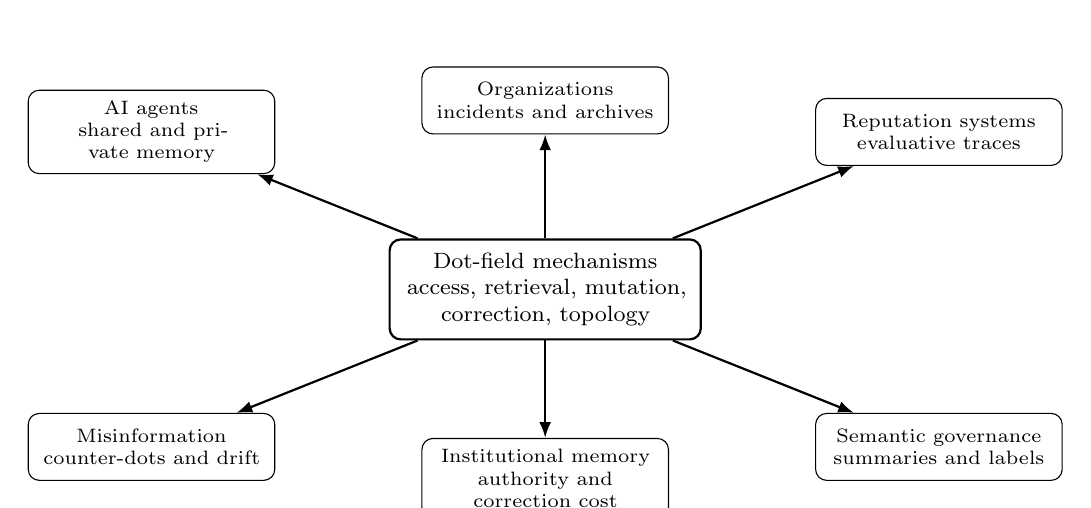
\begin{tikzpicture}[
  x=1cm,y=1cm,
  core/.style={draw, rounded corners, thick, align=center, text width=3.6cm, minimum height=1.0cm, font=\footnotesize, inner sep=5pt},
  app/.style={draw, rounded corners, align=center, text width=2.85cm, minimum height=0.85cm, font=\scriptsize, inner sep=4pt},
  arr/.style={-{Latex[length=2mm]}, thick}
]
\node[core] (core) at (0,0) {Dot-field mechanisms\\access, retrieval, mutation, correction, topology};
\node[app] (ai) at (-5,2.0) {AI agents\\shared and private memory};
\node[app] (org) at (0,2.4) {Organizations\\incidents and archives};
\node[app] (rep) at (5,2.0) {Reputation systems\\evaluative traces};
\node[app] (mis) at (-5,-2.0) {Misinformation\\counter-dots and drift};
\node[app] (inst) at (0,-2.4) {Institutional memory\\authority and correction cost};
\node[app] (sem) at (5,-2.0) {Semantic governance\\summaries and labels};
\foreach \x in {ai,org,rep,mis,inst,sem}{\draw[arr] (core) -- (\x);}
\end{tikzpicture}%
}
\caption{Application map. The same formal mechanisms appear across AI workspaces, organizations, reputation systems, misinformation settings, institutional archives, and semantic-governance problems. The applications differ in dominant mechanisms, observability, and governance burden.}
\label{fig:application-map}
\end{figure}

\subsection{AI multi-agent systems}\label{ai-multi-agent-systems}

AI agents increasingly operate in long-horizon, multi-session environments where a purely local memory stream is insufficient. A planning agent may remember its own prior actions, but a multi-agent workspace also requires shared task records, commitments, corrections, reputation traces, safety constraints, and institutional anchors such as project documents, issue trackers, policies, and logs. Dot-Trace Theory provides a schema for representing these objects without collapsing them into a single flat memory store.

In this setting, private dots correspond to an individual agent's stored experiences; public dots correspond to shared messages, task updates, and common records; institutional dots correspond to durable artifacts such as tickets, policies, logs, and canonical documents. The access graph determines which agents can retrieve which traces, while dot-dot relations encode support, contradiction, mutation, summary, or repair. This allows system designers to specify not only what agents remember, but also how shared memory is governed.

The practical value is auditability and control. If an AI agent refuses a request because it retrieves a negative safety dot, recommends a collaborator because it retrieves a competence dot, or changes strategy because it retrieves a postmortem dot, the system can expose the trace lineage behind that behavior. Dot-Trace Theory therefore supports transparent coordination, bounded memory, controlled forgetting, correction of stale memory, and explicit separation between private memory, shared memory, and institutional records.

\subsection{Organizational memory}\label{organizational-memory}

Organizations depend on records, stories, routines, postmortems, tickets, reputations, and informal recollections. Two teams with identical formal structure may behave differently because they carry different traces: one team remembers a previous outage as a process failure; another remembers the same event as an individual mistake; a third team has no accessible record at all. A model that only observes reporting structure or communication frequency misses this trace-mediated difference.

Dot-Trace Theory represents organizational memory as a distributed dot field. Meeting notes, incident reports, code reviews, audit logs, and informal narratives are dots with different provenance, accessibility, credibility, and decay rates. Summaries and dashboards are compressed dots. Policies and compliance records are institutional dots. Corrections, retractions, and revised postmortems are counter-dots or repair dots. The theory can therefore model how organizational knowledge is created, retained, distorted, institutionalized, or forgotten.

This framing is useful for diagnosing organizational failure. A team may fail not because knowledge is absent, but because the relevant dots are inaccessible, not credible, semantically compressed into a misleading label, or isolated in a different component of the organization. The access graph and dot graph make these distinctions explicit and allow interventions to target trace reach, provenance, and correction rather than only communication volume.

\subsection{Reputation and trust systems}\label{reputation-and-trust-systems}

Reputation is often represented as an aggregate score. Dot-Trace Theory treats such scores as downstream summaries of trace histories. A trust edge from $a_i$ to $a_j$ may be supported by positive dots about reliability, contradicted by negative dots about defection, strengthened by institutional certification, or weakened by testimonial dots from high-status sources. The reputation score is therefore not the primitive; the primitive is the set of accessible evaluative traces and their effective strengths.

This approach has two advantages. First, it makes reputation explainable: a system can identify which dots contributed to a reputation change, which sources transmitted them, and which counter-dots are available. Second, it distinguishes factual correction from social repair. A false negative dot may be corrected, but the trust edge it damaged may not automatically recover. Repair requires additional dots, repeated positive interactions, institutional exoneration, or bridge agents who can reintroduce corrected traces to affected components.

A dot-field account also clarifies why reputation systems can become brittle. If a compressed label dominates its source traces, agents may act on the label while losing access to the underlying evidence. If negative dots spread faster than counter-dots, exclusion risk may persist even after the original claim is weakened. Reputation governance therefore requires lineage, contestability, and limits on summary dominance.

\subsection{Misinformation and correction}\label{misinformation-and-correction}

Misinformation can be modeled as a dot whose epistemic quality is low but whose social effectiveness is high. A false dot may spread because it is salient, repeated, emotionally charged, transmitted by a trusted source, amplified by a bridge, or encoded into an institutional artifact. Dot-Trace Theory separates the truth of a trace from its accessibility, salience, credibility, and action impact.

Correction is therefore not merely the publication of true information. A counter-dot must reach the agents who hold the target dot, be retrieved in the relevant context, be credible to those agents, and semantically match the version of the dot they hold. If the false dot has mutated, a correction aimed at the original version may fail. If the false dot has already altered social topology, factual correction may still leave residual topology harm. These distinctions are central for studying rumor control, public retractions, scientific correction, institutional error, and reputation repair.

The theory also explains why late correction can be weaker than early correction. Once a misleading trace has become institutionalized, compressed into a label, or used to update trust edges, the correction must overcome not only belief but also access structure, social memory, and topology. Correction mechanisms therefore need timing, reach, semantic fit, and repair capacity.

\subsection{Institutional memory and governance}\label{institutional-memory-and-governance}

Institutional memory is a central application because institutions already maintain durable traces: policies, minutes, logs, contracts, tickets, reports, databases, and archives. Dot-Trace Theory asks when those traces become accessible, credible, action-relevant, and correction-resistant. This reframing clarifies both the value and the risk of institutional memory. It can synchronize action across time, but it can also preserve obsolete or biased traces with high authority.

Laws, contracts, archives, databases, policies, ledgers, and audit logs are institutionalized dots. They stabilize memory by slowing decay, widening access, raising default credibility, and attaching consequences to retrieval. Institutional memory can therefore improve coordination across time: agents can act on shared records rather than fragile private recollection.

The same mechanism creates risk. A false, biased, obsolete, or ambiguous institutional dot may become harder to correct precisely because it is durable, accessible, and authoritative. Dot-Trace Theory treats this as a governance problem. Institutions need not only storage but also contestability, lineage tracking, counter-dot procedures, correction logs, and mechanisms for distinguishing current authoritative records from superseded ones.

\subsection{Human-AI societies}\label{human-ai-societies}

Human-AI societies require special care because traces may be created by humans, generated by models, stored by platforms, summarized by agents, and retrieved by other agents or people. Dot provenance, mutation, and institutional anchoring become difficult but essential. The same trace may function as private memory for one agent, shared evidence for a team, and institutional record for a platform. A dot-field account makes these roles explicit rather than treating memory as an undifferentiated context window.

In human-AI systems, artificial agents may retrieve, summarize, recommend, and transmit traces at scales that humans cannot monitor directly. Dot-Trace Theory provides a vocabulary for specifying which traces are stored, who may access them, how they decay, how they can be challenged, and how they influence trust between humans and machines. It also clarifies why AI-generated summaries are not neutral containers: they are compressed dots that may become more retrievable than the source material.

This application creates a governance burden. Systems should distinguish human-authored dots from model-generated dots, source records from summaries, private traces from institutional traces, and current authoritative records from obsolete ones. Without those distinctions, artificial agents may amplify stale, biased, or uncorrected traces while appearing to provide coherent memory.

\subsection{Semantic governance and summarization}\label{semantic-governance-and-summarization}

Summarization, labeling, translation, and categorization are not merely text-processing operations in dot-field systems. They create compressed or mutated dots that can change what later agents retrieve and act upon. A meeting summary may become more authoritative than the meeting itself; a risk label may dominate the evidence from which it was produced; a translated account may shift the valence of a claim; and an automated memory condensation may erase a relevant exception.

Dot-Trace Theory treats these processes as semantic governance. A responsible system should record source links, compression rules, uncertainty, semantic drift, and correction paths. It should also evaluate whether compressed dots preserve action-relevant distinctions. If a summary becomes dominant while losing relevant detail, it can improve efficiency and simultaneously create behavioral compression loss.

\subsection{Application summary}\label{application-summary}

The applications differ in surface vocabulary but share the same formal structure. In each case, traces persist beyond events, agents have unequal access to them, retrieval affects action, and trace histories reshape social topology or institutional authority. The application question is therefore not whether dots exist in the abstract, but which dots are consequential, which mechanisms are active, which data make them observable, and which governance constraints are required.

This application logic also preserves claim discipline. A study of organizational memory should not automatically claim causal correction effects; a study of AI-agent memory should not automatically claim social-capital dynamics; and a study of misinformation should not infer semantic drift without observing or reconstructing dot lineages. Dot-Trace Theory supplies a common representation, but each application must specify its active mechanisms, observability grade, baselines, and ethical constraints.

\section{Differentiation From Adjacent Models}\label{differentiation-from-adjacent-models}

The distinct contribution of Dot-Trace Theory is not that it introduces agents, graphs, memory, reputation, or institutions as new topics. Each of those topics is already represented in established literatures. The contribution is a coupling: the theory makes persistent socially accessible traces into explicit state objects that connect agent action, memory, access, institutional record-keeping, social capital, and topology change. This distinction is important because otherwise the theory could be misread as a relabeling of existing models. It is not. It is a proposal about what must be represented when traces created by past events remain available, are retrieved in later contexts, and alter the structure through which future traces travel.

A useful way to state the boundary is by asking what each adjacent framework treats as primitive. In a standard multi-agent system, the primitives are agents, states, observations, policies, and actions. In social-network analysis, they are nodes, edges, and network positions. In temporal graph learning, they are evolving interactions and node or edge representations. In agent-memory systems, they are stored experiences and retrieval procedures. In collective-memory studies, they are shared recollections, narratives, and convergence processes. Dot-Trace Theory does not discard any of these primitives. Instead, it adds a trace object that can move among them: a dot may originate in an event, become stored memory, acquire social visibility, enter an institutional archive, support a reputation edge, mutate during transmission, or be defeated by a counter-dot.

\begin{figure}[htbp]
\centering
\resizebox{0.96\textwidth}{!}{%
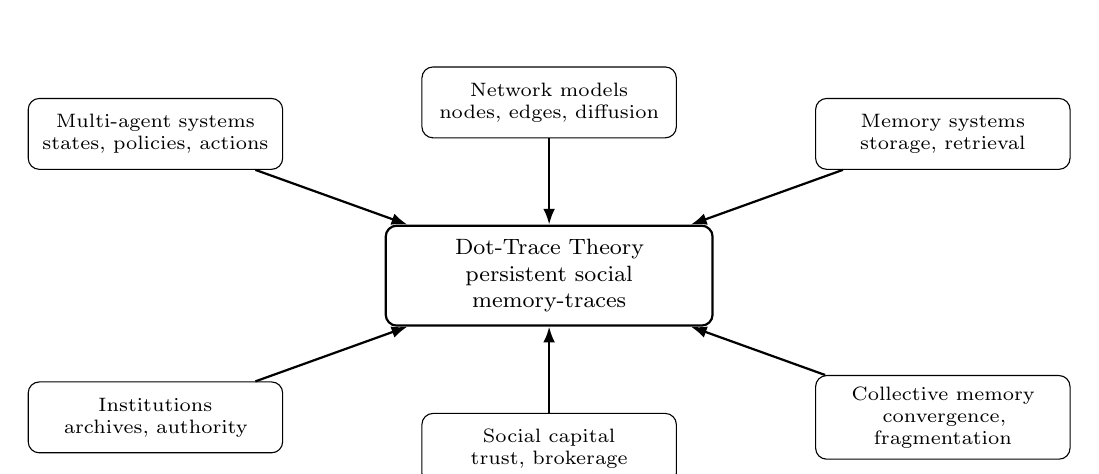
\begin{tikzpicture}[
  x=1cm,y=1cm,
  base/.style={draw, rounded corners, align=center, text width=2.95cm, minimum height=0.9cm, font=\scriptsize, inner sep=4pt},
  dot/.style={draw, rounded corners, thick, align=center, text width=3.8cm, minimum height=1.05cm, font=\footnotesize, inner sep=5pt},
  arr/.style={-{Latex[length=2mm]}, thick}
]
\node[base] (mas) at (-5.0,1.8) {Multi-agent systems\\states, policies, actions};
\node[base] (graph) at (0,2.2) {Network models\\nodes, edges, diffusion};
\node[base] (memory) at (5.0,1.8) {Memory systems\\storage, retrieval};
\node[dot] (dtt) at (0,0) {Dot-Trace Theory\\persistent social memory-traces};
\node[base] (inst) at (-5.0,-1.8) {Institutions\\archives, authority};
\node[base] (capital) at (0,-2.2) {Social capital\\trust, brokerage};
\node[base] (collective) at (5.0,-1.8) {Collective memory\\convergence, fragmentation};
\foreach \x in {mas,graph,memory,inst,capital,collective}{\draw[arr] (\x) -- (dtt);}
\end{tikzpicture}%
}
\caption{Differentiation by primitive object. Adjacent frameworks supply agents, edges, memory stores, institutions, social resources, and collective-memory processes. Dot-Trace Theory adds the persistent trace object that can move among these layers and thereby links them in a common state representation.}
\label{fig:differentiation-by-primitive}
\end{figure}


\begin{longtable}[]{@{}
  >{\raggedright\arraybackslash}p{0.19\textwidth}
  >{\raggedright\arraybackslash}p{0.23\textwidth}
  >{\raggedright\arraybackslash}p{0.27\textwidth}
  >{\raggedright\arraybackslash}p{0.25\textwidth}@{}}
\caption{Differentiation from adjacent frameworks.}\label{tab:differentiation-adjacent}\\
\toprule
\textbf{Framework} & \textbf{Core object} & \textbf{What it captures} & \textbf{What Dot-Trace Theory adds}\\
\midrule
\endfirsthead
\toprule
\textbf{Framework} & \textbf{Core object} & \textbf{What it captures} & \textbf{What Dot-Trace Theory adds}\\
\midrule
\endhead
Multi-agent systems & Agents, observations, states, actions, policies. & Decision-making, coordination, planning, equilibrium, and interaction. & Persistent traces with provenance, access, retrieval, credibility, and later topology effects.\\
Social-network analysis & Nodes, edges, positions, centrality, communities. & Relational structure, diffusion pathways, brokerage, cohesion, and inequality. & The trace-level memory substrate supporting edges, reputations, obligations, and repair.\\
Temporal graph learning & Timed events, evolving edges, node memories, embeddings. & Prediction on dynamic graphs and representation learning from event streams. & Semantic, institutional, and contestable trace objects rather than only events or latent embeddings.\\
Generative-agent memory & Memory streams, reflection, retrieval, planning. & Believable agent behavior and long-horizon coherence. & Social distribution of memories, agent-dot access, public/institutional traces, and topology feedback.\\
Graph-based memory & Memory nodes, relations, graph traversal. & Structured retrieval and relational memory organization. & Separation of agent-agent, dot-dot, and agent-dot access graphs, with social consequences.\\
Collective-memory research & Shared remembering, narratives, mnemonic convergence. & How communication and social topology shape group memory. & A formal dot field with access, mutation, counter-dots, institutional anchors, and measurable overlap.\\
Opinion dynamics & Beliefs, influence matrices, averaging, disagreement. & Conditions for consensus, polarization, or stable disagreement. & Structured trace weights and retrieval-dependent action rather than scalar opinion alone.\\
Social-capital theory & Resources available through durable relations. & Trust, obligation, brokerage, bonding, bridging, reputation. & A mechanism for how such resources are accumulated and lost through accessible traces.\\
\bottomrule
\end{longtable}

The central claim is therefore deliberately bounded. Dot-Trace Theory is not a universal replacement for these frameworks. It is useful when a system contains trace-mediated path dependence: past interactions create objects that persist, become accessible or inaccessible, are retrieved, are interpreted, and change future action or relations. If all transition-relevant information is already captured by a reduced agent-edge state, the dot-field representation is unnecessary for that modeling task. If trace access, retrieval, or mutation changes future behavior, the reduced representation is potentially incomplete.


\section{Ethical and Governance Considerations}\label{ethical-governance-considerations}

Dot-Trace Theory is ethically sensitive because it represents social memory, reputation, access, correction, and forgetting. A model that explains how traces shape behavior can also be used to manipulate visibility, amplify reputational harm, infer private beliefs, or suppress counter-dots. Governance is therefore not an optional afterthought. It is part of responsible dot-field design.

\begin{figure}[htbp]
\centering
\resizebox{0.92\textwidth}{!}{%
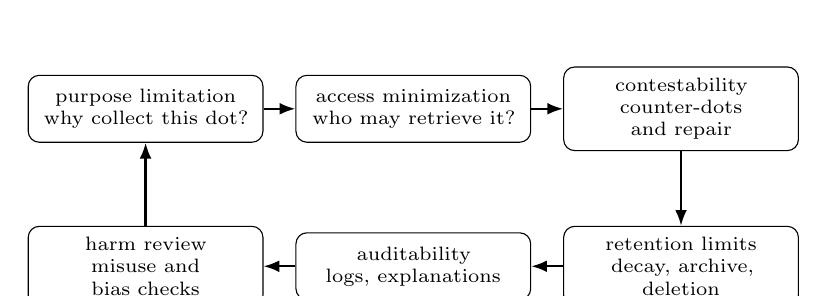
\begin{tikzpicture}[
  x=1cm,y=1cm,
  box/.style={draw, rounded corners, align=center, text width=2.7cm, minimum height=0.85cm, font=\scriptsize, inner sep=4pt},
  arr/.style={-{Latex[length=2mm]}, thick}
]
\node[box] (purpose) at (0,0) {purpose limitation\\why collect this dot?};
\node[box] (access) at (3.4,0) {access minimization\\who may retrieve it?};
\node[box] (contest) at (6.8,0) {contestability\\counter-dots and repair};
\node[box] (retain) at (6.8,-2.0) {retention limits\\decay, archive, deletion};
\node[box] (audit) at (3.4,-2.0) {auditability\\logs, explanations};
\node[box] (review) at (0,-2.0) {harm review\\misuse and bias checks};
\draw[arr] (purpose) -- (access); \draw[arr] (access) -- (contest); \draw[arr] (contest) -- (retain); \draw[arr] (retain) -- (audit); \draw[arr] (audit) -- (review); \draw[arr] (review) -- (purpose);
\end{tikzpicture}%
}
\caption{Governance loop for dot-field systems. Responsible trace modeling requires purpose limitation, access control, contestability, retention limits, auditability, and periodic harm review. Each governance control maps to a formal dot-field mechanism.}
\label{fig:governance-loop}
\end{figure}

A dot-field model can improve accountability, coordination, institutional learning, and correction. It can also support surveillance, reputational control, manipulation, exclusion, and automated memory-based sanction. Ethical analysis is therefore intrinsic to the theory. A system that formalizes socially consequential traces must specify who may create them, who may access them, how they may be challenged, when they should decay, and how harms are audited.

\subsection{Privacy and consent}\label{privacy-consent}

Dots can encode sensitive information: conflict, health status, political association, performance failure, disciplinary history, interpersonal evaluations, inferred beliefs, social ties, or private communications. Consent should therefore be tied not only to collection but also to persistence, access, reuse, mutation, and institutionalization. A trace that was acceptable in a private conversation may become harmful when archived, searchable, or used by automated agents in later decisions.

Responsible implementations should distinguish private, shared, institutional, and public traces. Access should be purpose-limited, role-sensitive, and time-bounded where the setting requires it. The fact that a dot improves prediction is not sufficient reason to retain or expose it. This is especially important for inferred dots, such as reputation labels, risk profiles, or behavioral summaries, because the affected agent may not know that the trace exists.

\subsection{Contestability and correction}\label{contestability-correction}

Because dots can shape reputation and access, affected agents require plausible routes to discover, challenge, contextualize, and repair harmful traces. Contestability includes the ability to inspect provenance, add counter-dots, request review, correct institutional records, and seek repair for residual topology harm. A correction mechanism that exists only formally is insufficient if the counter-dot cannot reach the agents or institutions that continue to act on the original trace.

Correction should be trace-specific and lineage-aware. Removing a conclusion without addressing its supporting dots may leave the same inference available through another path. Conversely, correcting a source dot may not correct all mutated, compressed, or institutional descendants. Governance procedures should therefore track lineages, descendant summaries, institutional anchors, and high-salience labels.

\subsection{Proportionality and forgetting}\label{proportionality-forgetting}

Persistent traces can become disproportionate. A single mistake may generate a durable negative dot that continues to affect opportunities long after the original context has changed. Proportionality requires that persistence and access be matched to legitimate use. Some traces should decay quickly, some should remain private, some should be archived but not surfaced by default, and some should be deleted or sealed after correction or expiration.

Forgetting is not always deletion. It may involve lowering salience, restricting access, adding context, superseding an old dot with a more recent one, or preserving the trace only in an audit archive. The appropriate mechanism depends on the domain, legal constraints, institutional function, and harm of continued retrieval. Dot-Trace Theory treats forgetting as a governance mechanism, not as a failure of memory.

\subsection{Auditability}\label{auditability}

Dot-induced decisions should be auditable when they affect trust, access, opportunity, discipline, visibility, or reputation. An audit should be able to reconstruct which records created a dot, which agents accessed it, which retrieval event made it active, which decision or edge update it influenced, and whether counter-dots or repair dots were available.

Auditability also constrains model evaluation. A dot-field system that improves prediction while hiding provenance or access paths is not governance-ready. Audit logs, lineage records, correction histories, and extraction uncertainty are part of the scientific and ethical artifact, not optional metadata. Without this chain, affected agents and external reviewers cannot contest harmful dots or evaluate whether a model's explanation is faithful.

\subsection{Misuse risk}\label{misuse-risk}

The same representation that supports epistemic resilience can support influence operations. If a system identifies which dots are central, credible, salient, and well-positioned for transmission, it can be used to manipulate memory, seed reputational harm, target bridge agents, poison institutional records, or suppress counter-dots. Misuse risk is highest when dot-field analytics are combined with asymmetric visibility, weak contestability, and automated topology updates.

Applications should report safeguards alongside performance metrics. Appropriate safeguards may include access minimization, red-team evaluation, negative-control audits, fairness analysis, contestability procedures, retention limits, and independent review for high-stakes uses. The theory's ability to model trace-mediated influence is valuable only when paired with constraints on how that influence is operationalized.

\section{Limitations}\label{limitations}

Dot-Trace Theory is intentionally broad: it is designed to represent trace-mediated dynamics across human, artificial, organizational, and hybrid systems. Breadth is useful only if it is paired with disciplined boundaries. The following limitations identify where the theory requires careful measurement, explicit assumptions, or narrower domain models. They are not defects to be hidden; they are conditions under which the theory should be applied cautiously.

First, dot identification is a substantive measurement problem. Real events do not arrive pre-segmented into clean traces. A meeting, accident, conversation, post, or model output may generate multiple candidate dots, and different agents may encode the same event differently. The measurement protocol therefore requires a dot test, identity rules, and uncertainty reporting. Without those constraints, the analyst can over-extract traces and inflate apparent explanatory power.

Second, dot identity can change during transmission. A trace may be translated, summarized, reframed, exaggerated, institutionalized, or embedded into an AI memory store. The same lineage may preserve task-relevant identity in one setting and lose it in another. Applications that study mutation or correction must specify whether identity is token-based, lineage-based, semantic, or behavioral. Otherwise, a correction may appear to fail simply because the measured counter-dot targets a different version of the trace.

Third, not every persistent trace is consequential. Some dots are low-salience, low-credibility, inaccessible, redundant, or irrelevant to the modeled decision. Dot-Trace Theory therefore does not imply that every message, memory, or record should be retained as a causal variable. Practical models require thresholds, decay rules, retrieval constraints, salience functions, and principled compression. A full dot field may be conceptually richer than a reduced state while being empirically or computationally unnecessary for a particular outcome.

Fourth, credibility and salience are difficult to estimate. Human agents do not update credibility according to a single rational rule; AI agents may rank memories according to system-specific retrieval mechanisms; institutions may confer authority unevenly. Treating credibility as directly observed when it is merely inferred can produce misleading conclusions. Empirical work should distinguish observed authority labels, measured retrieval frequencies, inferred credibility, and latent belief.

Fifth, dot fields can become computationally large. If every interaction creates multiple persistent traces, the state space can grow quickly. Scalable implementations require indexing, pruning, approximate retrieval, summarization, and archiving. These operations are themselves dot-field mechanisms because they change which traces remain visible and action-relevant. Computational efficiency is therefore not only an engineering concern; it can alter the social dynamics being modeled.

Sixth, external validity is domain-specific. A mechanism demonstrated in a synthetic agent society, a collaborative software platform, or an organizational incident database does not automatically generalize to open social media, legal institutions, political communication, or interpersonal trust. Each domain has distinct access regimes, institutional authorities, privacy constraints, and correction pathways. The theory provides a formal vocabulary and conditional results; empirical validation must be performed within particular settings.

Seventh, dot-field modeling is ethically sensitive. Representing traces, access, reputation, correction, and forgetting can support accountability and repair, but it can also support surveillance, manipulation, exclusion, and reputational control. The governance section of the paper is therefore part of the theory's responsible-use boundary. A high-performing dot-field model is incomplete if affected agents cannot inspect, contest, correct, or contextualize consequential traces.

\begin{longtable}{L{0.20\textwidth}L{0.31\textwidth}L{0.37\textwidth}}
\caption{Major limitations and corresponding safeguards.}\label{tab:limitations-safeguards}\\
\toprule
\textbf{Limitation} & \textbf{Risk} & \textbf{Required safeguard}\\
\midrule
\endfirsthead
\toprule
\textbf{Limitation} & \textbf{Risk} & \textbf{Required safeguard}\\
\midrule
\endhead
Dot identification & Over-extraction or under-extraction of traces. & Apply the minimum dot test, report coder reliability, and distinguish observed from inferred dots.\\
Dot identity drift & Treating mutated descendants as unchanged originals. & Specify token, lineage, semantic, or behavioral identity and report semantic-fidelity thresholds.\\
Low consequentiality & Modeling noise as causal structure. & Use salience, accessibility, retrieval, and prediction-lift checks before asserting mechanism relevance.\\
Credibility estimation & Confusing authority labels, belief, and retrieval rank. & Separate observed source status from inferred credibility and test alternative credibility models.\\
State growth & Computational overload and unprincipled pruning. & Use audited compression, bounded truncation, and sensitivity tests for omitted dot mass.\\
External validity & Overgeneralization across domains. & Match claims to observability grade, domain mechanisms, and held-out validation settings.\\
Ethical sensitivity & Surveillance, manipulation, or reputational harm. & Require purpose limitation, access control, contestability, correction, forgetting, and auditability.\\
\bottomrule
\end{longtable}

These limitations establish a practical standard for use. The strongest version of a dot-field claim requires three forms of support: a formal mechanism showing why traces matter, a measurement design showing that the relevant traces can be observed or validly inferred, and a validation design showing that dot-field information improves explanation, prediction, or intervention relative to appropriate reduced baselines. When any of these supports is missing, the claim should be correspondingly weaker.

\section{Cross-Section Consistency and Claim Discipline}\label{cross-section-consistency-claim-discipline}

Dot-Trace Theory operates across several levels of abstraction: ontology, dynamics, theorems, measurement, implementation, validation, applications, and governance. Because the same object can appear under different empirical names--a memory, record, post, ticket, rumor, policy, or summary--the article maintains three consistency rules.

First, claims are stated at the weakest level that supports them. A formal result about $\Omega_t^{aug}$ is not automatically an empirical claim about a particular dataset. A measurement protocol may justify claims about observed dots, but not about latent private retrieval unless additional assumptions or instruments are supplied. A simulator can test whether mechanisms are internally coherent, but it does not by itself establish that the same mechanisms operate in an external domain.

Second, the theory distinguishes representation from endorsement. A dot may be true, false, incomplete, biased, obsolete, or contested. Representing a dot in the state does not imply that the dot is accepted as accurate or normatively legitimate. This distinction is especially important for reputational, institutional, and correction-sensitive applications, where the act of storing or surfacing a trace can itself affect social outcomes.

Third, mechanism-specific claims require mechanism-specific evidence. A positive prediction lift for a dot-field model supports the value of trace variables, but it does not by itself identify whether the effect came from retrieval, transmission, mutation, institutionalization, correction, compression, or topology feedback. The validation protocol therefore pairs prediction tests with ablations, negative controls, observability grades, and mechanism-specific diagnostics.

These rules connect the formal and operational parts of the paper. The theorem spine establishes why dot-field variables can matter. The measurement protocol defines when those variables can be observed or estimated. The implementation and simulator sections specify how dot-field mechanisms can be executed. The validation framework tests whether those mechanisms add predictive or explanatory value relative to reduced baselines. The governance sections specify how trace-sensitive systems should be constrained when dots affect reputation, access, or institutional authority.

\section{Discussion: Research Uses and Integration}\label{discussion-research-uses-integration}

The preceding sections establish Dot-Trace Theory as a general representation for trace-mediated social systems. This discussion clarifies how the theory can be used without weakening its claim discipline. The theory is not meant to replace domain-specific models of interaction, cognition, institutions, or communication. It supplies a state vocabulary and a set of mechanism interfaces for cases in which persistent traces remain consequential after the current social graph and current agent attributes have been observed.

A first use is \emph{diagnostic}. In many systems, analysts can observe social edges and current actions but cannot explain why superficially similar relations evolve differently. The diagnostic question is whether the difference is carried by accessible traces: prior betrayals, commitments, documents, recommendations, accusations, repairs, summaries, or institutional records. A dot-field analysis asks which traces exist, who can access them, how they are weighted, whether they are linked to counter-dots or institutional anchors, and whether they exert edge pressure on future relations. Under this use, the theory functions as a language for locating hidden state variables that ordinary agent-edge descriptions may omit.

A second use is \emph{comparative}. Dot-Trace Theory makes it possible to compare social systems by trace structure rather than only by social topology. Two teams, platforms, or artificial-agent societies may have similar interaction graphs but different dot fields. One may preserve institutional records, another may rely on private memory; one may expose corrections widely, another may trap corrections behind weakened ties; one may compress events into reputational labels, another may preserve detailed provenance. These differences affect convergence, fragmentation, correction, and social capital. The theory therefore supports comparison along dimensions such as archival reach, correction reach, semantic drift, access inequality, and topology-memory coupling.

A third use is \emph{generative}. The mixed-mechanism model specifies how to construct simulated or computational societies in which agents do not merely exchange messages but create, retrieve, transform, contest, and institutionalize traces. This use is most appropriate when the objective is to study mechanism behavior under controlled assumptions: whether bridges accelerate convergence, whether correction fails under semantic drift, whether institutionalization increases persistence and correction cost, or whether recursive topology feedback produces exclusion. Such simulations do not by themselves validate the theory externally, but they test internal coherence and generate observable signatures for empirical work.

A fourth use is \emph{measurement-oriented}. The extraction protocol turns the conceptual primitive into a coding task: identify candidate traces, test them against content, persistence, provenance, access, and action relevance, and then code uncertainty. This use is central because the theory's empirical value depends on whether dots can be observed or reconstructed with sufficient reliability. The observability ladder prevents overclaiming: a study with action-only data can support weaker pressure-level claims, whereas a study with provenance, access, retrieval, and correction logs can support stronger dot-field claims.

A fifth use is \emph{governance-oriented}. Once traces are treated as causal objects, systems that store, rank, summarize, or expose traces become normatively significant. Reputation records, incident reports, institutional archives, shared memory systems, and long-term memories in artificial agents can influence access, trust, and exclusion. Dot-Trace Theory therefore links modelling to governance: persistent traces require contestability, correction channels, provenance, proportional retention, and auditability. These requirements are not merely ethical additions; they are implied by the theory's own claim that dots can alter future social topology.

\begin{table}[htbp]
\centering
\small
\renewcommand{\arraystretch}{1.25}
\begin{tabular}{L{0.20\textwidth}L{0.32\textwidth}L{0.34\textwidth}}
\toprule
Use of the theory & Central question & Appropriate evidence or output\\
\midrule
Diagnostic & What trace variables are missing from a reduced state description? & Dot inventory, access map, retrieval evidence, edge-pressure reconstruction.\\
Comparative & How do systems differ in trace structure, not only in social topology? & Measures of dot overlap, correction reach, archival reach, semantic drift, and topology-memory coupling.\\
Generative & What dynamics arise when trace mechanisms are activated under controlled assumptions? & Mechanism-specific simulations, ablations, negative controls, and sensitivity analysis.\\
Measurement-oriented & Can dots, access, provenance, and relations be observed or reliably inferred? & Extraction protocol, observability grade, reliability metrics, uncertainty reporting.\\
Governance-oriented & How should systems manage traces that affect reputation, access, and exclusion? & Provenance, retention rules, contestability, audit logs, correction pathways, misuse controls.\\
\bottomrule
\end{tabular}
\caption{Research uses of Dot-Trace Theory. The same formal vocabulary supports diagnostic, comparative, generative, measurement-oriented, and governance-oriented uses, but each use requires a different evidentiary standard.}
\label{tab:research-uses-integration}
\end{table}

This integration clarifies why the theory is layered. The ontology defines what is represented. The theorem spine establishes why representation matters and how dot dynamics can behave. The measurement protocol specifies when the objects can be studied empirically. The implementation and simulator sections show how the theory can be executed under explicit assumptions. The validation framework determines whether dot-field variables improve prediction or explanation relative to reduced baselines. The governance sections identify obligations that arise when traces become consequential. The result is a structured theory that can be specialized for mathematical analysis, empirical coding, agent-system design, or institutional governance.

\section{Boundary Conditions and Extensions}\label{boundary-conditions-extensions}

Dot-Trace Theory is intended for systems in which persistent traces mediate action. Its usefulness depends on whether the relevant traces can be represented, measured, and connected to outcomes. The theory therefore has explicit boundary conditions. These boundaries are not merely limitations; they are part of the theory's claim discipline. A dot-field model should be used when it captures transition-relevant trace structure that reduced representations omit. It should be avoided, simplified, or treated as descriptive when those conditions do not hold.

\subsection{When dot fields are unnecessary}\label{boundary-memoryless-sufficient-state}

A dot-field representation is unnecessary when the reduced state is already sufficient for the outcome and horizon being modeled. Formally, for a reduced state
\[
Z_t=(A,E_t,X_t,\bar S_t),
\]
the dot field adds no predictive information for $Y_{t+1}$ when
\[
I(Y_{t+1};D_t,R_t^D,B_t,\mathbf M_t,Q_t,L_t\mid Z_t)=0.
\]
In such cases, dots may still be descriptively meaningful, but they are not required for the transition model. Examples include short-horizon systems where prior traces are irrelevant, settings where current edge weights already encode all consequential history, or tasks where outcomes are driven by exogenous shocks rather than memory, reputation, correction, or institutional records.

This boundary is important because it prevents universalizing the theory. Dot-Trace Theory does not claim that every social system requires an explicit trace layer. It claims that when traces remain action-relevant after conditioning on the reduced state, omitting them can produce representational and predictive loss.

\subsection{When dot fields are difficult to measure}\label{boundary-measurement-limits}

The theory is also bounded by observability. Many socially important traces are private, implicit, strategically hidden, or reconstructed after the fact. A researcher may observe an action and infer that a memory was relevant, but such inference is weaker than observing access, retrieval, or communication directly. Applications should therefore state the observability grade of the data and distinguish observed dots from inferred or latent dots.

Weak observability does not make the theory useless, but it changes the kind of claim that can be made. Action-only data may support an aggregate edge-pressure interpretation, but they cannot uniquely identify which dots produced that pressure. Communication logs may reveal transmitted traces but not private retrieval. Institutional archives may reveal durable records but not whether agents noticed them. High-stakes claims about credibility, correction reach, semantic drift, or social liability require stronger measurement than claims about aggregate prediction lift.

\subsection{When mechanisms are inactive or dominated}\label{boundary-mechanism-limits}

A dot-field model may be formally available but mechanistically unnecessary if the relevant dot processes are inactive. In some systems, dots may persist but not transmit; transmit but not mutate; mutate but not affect action; or affect action without altering topology. The active mechanism set should therefore be identified rather than assumed. Mechanism ablation, negative controls, and matched reduced models are essential for determining whether retrieval, access, mutation, institutionalization, correction, or topology feedback is actually doing explanatory work.

The theory is also bounded by mechanism dominance. In a given domain, one mechanism may dominate the others. For example, institutional anchoring may overwhelm private memory, platform ranking may dominate interpersonal transmission, or high-authority testimonials may dominate semantic fit. Such cases do not refute the theory; they specify which dot processes are most consequential in that domain. A well-specified application should therefore report not only whether dot variables matter, but which dot mechanisms carry the effect.

\subsection{Computational and design boundaries}\label{boundary-computational-design}

Dot fields can become large. Each event can create multiple traces; each trace can have access relations, semantic links, lineages, credibility estimates, and lifecycle variables. Without bounded retrieval, canonicalization, pruning, compression, and audit logs, a computational implementation may become expensive, opaque, or unstable. The algorithmic sections therefore treat dot-field modeling as a typed architecture rather than as unbounded memory accumulation.

A practical system should specify its memory budget, retrieval horizon, archive policy, compression rules, correction procedure, and auditability requirements. These design choices are not merely engineering details. They determine which dots can influence future action and which dots disappear from the effective state. A system with aggressive compression may become efficient but lose action-relevant distinctions; a system with extensive archival memory may preserve accountability but increase privacy and correction burdens.

\subsection{Normative and governance boundaries}\label{boundary-governance-limits}

The theory is truth-neutral and value-neutral at the level of representation: a dot can be accurate or false, fair or biased, protective or harmful. That neutrality is useful for modeling, but it creates governance obligations. A trace that persists and affects reputation may require contestability. A trace that becomes institutionalized may require correction pathways. A trace that changes access to opportunities may require proportionality and accountability. Systems that operationalize dot fields should therefore include access controls, retention limits, uncertainty labels, correction logs, and audit procedures.

The governance boundary is especially important for human-AI systems. An AI workspace that stores private evaluations, compressed summaries, or institutional memory can create durable social consequences even when no human intends a formal judgment. Dot-Trace Theory helps make those consequences visible, but it does not by itself determine whether a dot should be stored, surfaced, or acted upon. That decision requires domain-specific ethical and legal standards.

\subsection{Extensions}\label{boundary-extensions}

Several extensions follow naturally from the core framework. First, dot fields can be connected to causal-inference designs by treating access, retrieval, correction, or institutionalization as interventions. Second, semantic representations can be strengthened by using richer models of entailment, contradiction, and pragmatic context. Third, the social-capital module can be specialized for organizations, online platforms, scientific communities, or human-AI teams. Fourth, recursive feedback stability can be extended to multiplex graphs in which trust, authority, communication, and obligation edges evolve differently. Fifth, the measurement protocol can be developed into domain-specific codebooks for collaborative software, incident management, scientific peer review, or controlled group experiments.

These extensions should preserve the central discipline of the theory: state the trace object, define access, identify active mechanisms, specify assumptions, report observability, and test dot-field value against reduced baselines. The goal is not to expand the theory without limit, but to use its core representation to build precise domain models.

\section{Conclusion}\label{conclusion}

Dot-Trace Theory develops a formal language for systems in which agents, memory, and social topology co-evolve through persistent traces. Its primitive object is the dot: a socially situated memory-trace created by an event, observation, interaction, claim, evaluation, or record. Its central state object is the dot field: a coupled structure containing agents, social edges, dots, dot-dot relations, access relations, memory weights, provenance lineages, institutional anchors, correction states, and related variables required to model trace-mediated action.

The main contribution is representational. In memory-sensitive social systems, a reduced agent-edge state may omit the traces agents retrieve and act upon. Dot-Trace Theory specifies when that omission matters: dot-field variables are necessary when they contain transition-relevant information not encoded in the reduced state. The theory also specifies the reciprocal boundary: if the reduced state already contains a sufficient statistic for the relevant traces, an explicit dot field may be unnecessary for that task.

The formal results show how this representational claim extends into dynamics. Dot exchange can generate collective convergence or fragmented memory. Temporal sequencing can make the same set of traces produce different interpretations. Institutional dots can stabilize memory while increasing correction costs. Evaluative dots can reshape trust, reputation, alliance, and exclusion. Counter-dots can correct false or obsolete traces only when they have sufficient reach, credibility, and semantic fit. Mutation and compression can create drift, labels, and correction mismatch. Recursive topology-access-memory feedback can stabilize, amplify, or close off corrective exposure depending on the strength of the feedback channel.

The operational sections show what is required to use the theory responsibly. Dots must be extracted with explicit criteria; access must be distinguished from attention and retrieval; credibility and salience must be treated as uncertain; implementations must be bounded, typed, and auditable; validation must compare dot-field models against reduced baselines and negative controls; and high-stakes applications must provide contestability, correction, proportionality, and retention limits. These requirements are not external additions to the theory. They follow from treating persistent traces as causal objects.

Dot-Trace Theory is not a replacement for multi-agent systems, social-network analysis, collective-memory research, social-capital theory, institutional-memory studies, or dynamic graph learning. It is a bridge among them. Its explanatory value depends on disciplined use of its core distinctions: access versus retrieval, representation versus endorsement, and mechanism-specific evidence versus aggregate prediction lift. It gives formal status to the traces that social systems leave behind and later act upon. By making those traces explicit, the theory provides a basis for analyzing how social memory is created, distributed, contested, institutionalized, compressed, corrected, and transformed into future action.


The central methodological implication is that social memory should be modelled neither as a purely private cognitive store nor as a mere attribute of the social graph. In trace-mediated systems, memory is distributed across agents, artifacts, institutions, platforms, and communicative paths. A theory of such systems must therefore represent both the traces themselves and the social conditions under which they become accessible, retrievable, authoritative, contested, or forgotten. Dot-Trace Theory provides one formal route for doing so.
\appendix

\section{Glossary}\label{appendix-glossary}

\textbf{Access graph:} The bipartite graph $G_t^B=(A,D_t,B_t)$ connecting agents to dots they can access. Access is not the same as attention or retrieval.

\textbf{Dot-induced edge pressure:} The aggregate pressure $\zeta_{ij}(t)$ created when agent $a_i$ retrieves evaluative dots about agent $a_j$. It is distinct from the reduced state $Z_t$.

\textbf{Accessible dot set:} The set $\mathcal M_i(t)=\{d\in D_t:(a_i,d)\in B_t\}$ of dots available to agent $a_i$ at time $t$.

\textbf{Archival social capital:} Advantage generated by access to durable institutional dots such as records, logs, policies, archives, tickets, contracts, or validated reports.

\textbf{Collective memory convergence:} Increasing similarity among agents' accessible dot sets, retrieved dot sets, or dot-weight vectors.

\textbf{Compressed dot:} A dot produced by summarizing, abstracting, or aggregating a set of source dots. A compressed dot may be useful, but it can also erase action-relevant distinctions.

\textbf{Counter-dot:} A dot that contradicts, weakens, qualifies, or reframes another dot.

\textbf{Correction pressure:} The effective force of accessible, retrieved, credible, and well-targeted counter-dots against a target dot.

\textbf{Correction reach:} The share of agents for whom a counter-dot has positive effective counter-strength.

\textbf{Dot:} A persistent, socially situated memory-trace created by an event, observation, interaction, claim, evaluation, or record.

\textbf{Dot-centroid:} A dot that minimizes average access distance to a group in the lifted heterogeneous graph $H_t=(A\cup D_t,E_t\cup R_t^D\cup B_t)$.

\textbf{Dot decay:} Decline in dot weight, salience, credibility, accessibility, or retrieval probability over time.

\textbf{Dot field:} The coupled state containing agents, dots, social edges, dot relations, access relations, environment, and relevant memory, lineage, institutional, and correction variables.

\textbf{Dot graph:} The graph $G_t^D=(D_t,R_t^D)$ of relations among dots, including support, contradiction, lineage, similarity, compression, or temporal precedence.

\textbf{Dot institutionalization:} Encoding a dot into a durable artifact, record, archive, rule, policy, database, ledger, or formal system.

\textbf{Dot mutation:} Transformation of a dot during transmission, reinterpretation, summarization, translation, or reframing.

\textbf{Dot overlap:} Shared dot access or shared dot-weight similarity between agents or groups.

\textbf{Dot salience:} The importance or retrieval strength of a dot in a decision context.

\textbf{Dot visibility:} The degree to which a dot is accessible across a social system.

\textbf{Dot-field projection:} A mapping from a richer dot-field state to a reduced representation, such as the agent-edge state. Projection can remove transition-relevant trace information.

\textbf{Dot-induced topology:} Changes in social edges caused by retrieved dots and their evaluative pressure.

\textbf{Dot-mediated social capital:} Expected actionable advantage generated by access to valuable dots, favorable evaluative traces, institutional records, semantic brokerage, correction capacity, and reduced dot liabilities.

\textbf{Effective retrievable strength:} The action-relevant strength of a dot for an agent, typically combining access, memory weight, credibility, salience, and retrieval probability.

\textbf{Edge pressure:} The aggregate positive or negative force exerted by retrieved evaluative dots on a particular social edge.

\textbf{Epistemic resilience:} A group's capacity to reduce active error margins created by false, obsolete, or misleading dots through accessible and effective counter-dots.

\textbf{Evaluative dot:} A dot that assigns positive, negative, or neutral social value to an agent, action, role, institution, or relation.

\textbf{Institutional dot:} A dot encoded into a durable artifact or institution, such as a policy, archive, database, ledger, ticket, record, or official report.

\textbf{Lineage:} The ancestry relation connecting a dot to prior dots, events, transmissions, mutations, or compressions from which it descends.

\textbf{Lifted heterogeneous graph:} The graph $H_t=(A\cup D_t,E_t\cup R_t^D\cup B_t)$ that contains both agents and dots as vertices.

\textbf{Memory-action coupling:} The principle that retrieved dots influence agent action.

\textbf{Memory barycenter:} A vector-space aggregate of agents' dot-weight vectors, used to represent collective memory when dot weights are comparable across agents.

\textbf{Repair dot:} A dot created after correction that supplies positive trust, reputation, or topology pressure to repair residual social harm.

\textbf{Residual topology harm:} Persistent damage to social edges, access, or reputation that remains after factual correction of a target dot.

\textbf{Reputation capital:} Positive social advantage generated by favorable evaluative dots and the edges they sustain.

\textbf{Semantic brokerage capital:} Advantage generated by controlling or authenticating the translation, summarization, reframing, or anchoring of dots across agents or groups.

\textbf{Social-dot coupling:} The relationship between social tie strength and dot similarity.

\textbf{Social liability:} Negative social disadvantage generated by unfavorable evaluative dots and the edges they weaken or remove.

\textbf{Topology-mediated social capital:} Expected advantage generated by dot-induced changes in an agent's social position.

\textbf{Trace-mediated path dependence:} Dependence of future action or topology on persistent traces created by prior events rather than on the current agent-edge state alone.

\clearpage
\phantomsection
\addcontentsline{toc}{section}{References}
\bibliographystyle{plainnat}
\bibliography{references}

\end{document}
